% !TeX spellcheck = en_US

\newglossaryentry{pseudoinverse}
{name={pseudoinverse},
  description={The \index{pseudoinverse}Moore–Penrose pseudoinverse $\mA^{+}$ 
 	of a \gls{matrix} $\featuremtx \in \mathbb{R}^{\samplesize \times \nrfeatures}$ 
	generalizes the notion of an \gls{inverse} \cite{GolubVanLoanBook}. 
	The pseudoinverse arises naturally in \gls{ridgeregression} for a 
	\gls{dataset} with \gls{featuremtx} $\featuremtx$ and \gls{labelvec} 
	$\labelvec$ \cite[Ch.\ 3]{hastie01statisticallearning}. 
	The \glspl{modelparam} learned by \gls{ridgeregression} 
  	are given by
  	\[
  	\widehat{\weights}^{(\regparam)}  = \big(\featuremtx^{T} \featuremtx + \regparam \mI \big)^{-1} \featuremtx^{T} \vy, \quad \regparam > 0.
  	\]
  	We can then define the pseudoinverse $\featuremtx^{+} \in \mathbb{R}^{\nrfeatures \times \samplesize}$ via 
  	the limit \cite[Ch. 3]{benisrael2003generalized}
  	\[
  	\lim_{\regparam \to 0^+} \widehat{\weights}^{(\regparam)} = \featuremtx^+ \vy.
  	\]
	\\
	See also: \gls{matrix}, \gls{inverse}, \gls{ridgeregression}. },
 first={pseudoinverse},
 text={pseudoinverse}
}

\newglossaryentry{randomexperiment}
{name={random experiment},
	description={A random experiment\index{random experiment} is a physical (or abstract) process 
    	 	that produces an outcome $\outcome$ from a set $\samplespace$ of possibilities. 
	 	This set of all possible outcomes is referred to as the \gls{samplespace} of 
	 	the experiment. The key characteristic of a random experiment is that its 
	 	outcome is unpredictable (or uncertain). Any measurement or observation 
	 	of the outcome is a \gls{rv}, i.e., a \gls{function} of the outcome $\outcome \in \samplespace$. 
	 	\Gls{probability} theory uses a \gls{probspace} as a mathematical structure for the study of 
	 	random experiments. A key conceptual property of a random experiment is that it can 
	 	be repeated under identical conditions. Strictly speaking, repeating a random experiment 
	 	a given number of $\samplesize$ times defines a new random experiment. The outcomes 
	 	of this new experiment are length-$\samplesize$ sequences of outcomes 
	 	from the original experiment (see Fig. \ref{fig_randomexperiment_dict}). While the outcome of a single experiment is 
	 	uncertain, the long-run behaviour of the outcomes of repeated experiments 
	 	tends to become increasingly predictable. This informal claim can be made 
	 	precise via fundamental results of \gls{probability} theory, such as the \gls{lln} 
	 	and the \gls{clt}.
	 	\begin{figure}[H]
		\begin{center}
	 		\begin{tikzpicture}[>=Stealth, node distance=1.5cm and 2cm, every node/.style={font=\small}]
			\node (experiment) [draw, rectangle, rounded corners, minimum width=2.6cm, align=center] {random\\experiment};
			\node (omega) [right=of experiment] {$\outcome \in \samplespace$};
			\coordinate (rightpad) at ($(omega.east) + (0.2,0)$);
			\draw[->] (experiment) -- (omega);
			\node (sequence) [below=of experiment, yshift=-0.5cm] {$(\outcome^{(1)}, \,\outcome^{(2)}, \,\dots, \,\outcome^{(\samplesize)})$};
			\node (sequence1) [below=of sequence, yshift=-0.5cm] {$(\datapoint^{(1)}, \,\datapoint^{(2)}, \,\dots, \,\datapoint^{(\samplesize)})$};
			\draw[->, thick] (experiment.south) -- node[midway, right, xshift=3pt] {repeat $\samplesize$ times} (sequence.north);
			\draw[->, thick] (sequence.south) -- node[midway, right, xshift=3pt] {\glspl{rv}} (sequence1.north);
			% Anchor node ~60% along the repeat arrow
			\path (experiment.south) -- (sequence.north) coordinate[pos=0.6] (repeatpoint);
			% Dotted rounded box enclosing experiment and part of repeat arrow
        			\node[draw=black, rounded corners, dotted, fit={(experiment) (repeatpoint) (rightpad)}, inner sep=8pt, label=above:{new random experiment with $\samplespace' = \samplespace \times \ldots \times \samplespace$}] {};
	 		\end{tikzpicture}
	     	\end{center}
		\caption{A random experiment produces an outcome $\outcome \in \samplespace$ from a set 
		of possibilities (i.e., a \gls{samplespace}) 
		$\samplespace$. Repeating the experiment $\samplesize$ times yields another random 
		experiment, whose outcomes are sequences 
		$(\outcome^{(1)}, \,\outcome^{(2)}, \,\dots, \,\outcome^{(\samplesize)}) \in \samplespace\times\ldots\times \samplespace$. 
		One example of a random experiment arising in many \gls{ml} applications is the gathering 
		of a \gls{trainset} $\datapoint^{(1)},\,\ldots,\,\datapoint^{(\samplesize)}$. \label{fig_randomexperiment_dict}}
	 	\end{figure} 
	 	Examples for random experiments arising in \gls{ml} applications include the following: 
	 	\begin{itemize} 
			\item \Gls{data} collection: The \glspl{datapoint} collected in \gls{erm}-based methods 
			can be interpreted as \glspl{rv}, i.e., as \glspl{function} of the outcome $\outcome \in \samplespace$ 
			of a random experiment. 
			\item \Gls{stochGD} uses a random experiment at each iteration to select a subset of 
			the \gls{trainset}. 
			\item \Gls{privprot} methods use random experiments to perturb  
			the outputs of an \gls{ml} method to ensure \gls{diffpriv}. 
	 	\end{itemize} 
		See also: \gls{samplespace}, \gls{rv}, \gls{probability}, \gls{probspace}.},
 	firstplural={random experiments},
 	plural={random experiments},
 	first={random experiment},
 	text={random experiment}
}


\newglossaryentry{dimension}
{name={dimension},
	description={
	The \index{dimension}dimension $\dim \mathcal{A}$ of a 
	\gls{vectorspace} $\mathcal{A}$ is the cardinality of any 
	\gls{basis} of $\mathcal{A}$ \cite{StrangLinAlg2016}. 
	Strictly speaking, this definition applies only to finite-dimensional \glspl{vectorspace}, 
	i.e., those that possess a finite \gls{basis}. 
	\begin{figure}[H]
	\begin{tikzpicture}[scale=1]
  % Axes (optional; remove if you want it even more minimal)
  %	\draw[->, thin, gray] (-0.2,0) -- (3.2,0) node[right] {$\vw^{(1)}$};
  %	\draw[->, thin, gray] (0,-0.2) -- (0,3.2) node[above] {$\vw^{(1)}$};
  	\coordinate (O) at (0,0);
  % Basis 1: standard (solid)
  	\draw[->, thick] (O) -- (1.8,0) node[below right] {$\ve^{(1)}$};
  	\draw[->, thick] (O) -- (0,1.6) node[above left] {$\ve^{(2)}$};
  % Basis 2: rotated by ~45° (dashed)
\draw[->, thick, dashed, shift={(3.5,0.5)}] (0,0) -- (1.2,1.2) node[above right] {$\vu^{(1)}$};
\draw[->, thick, dashed, shift={(3.5,0.5)}] (0,0) -- (-1.2,1.2) node[above left] {$\vu^{(2)}$};
  % Basis 3: non-orthogonal / skewed (dotted)
  	\draw[->, thick, dotted, shift={(-2.5,-2.5)}] (O) -- (2.0,0.6) node[above right] {$\vw^{(1)}$};
  	\draw[->, thick, dotted, shift={(-2.5,-2.5)}] (O) -- (0.4,1.8) node[left] {$\vw^{(2)}$};
  % Simple legend
 % \node[anchor=west] at (1.6,-0.6) {\footnotesize \textbf{Bases:} solid = standard,\; 
 % dashed = rotated,\; dotted = skewed};
\end{tikzpicture}
\caption{Three \glspl{basis}, $\big\{\ve^{(1)},\ve^{(2)} \big\}, \big\{\vu^{(1)},\vu^{(2)} \big\},
\big\{\vw^{(1)},\vw^{(2)} \big\}$, for the \gls{vectorspace} $\mathbb{R}^{2}$.} 
\end{figure}
	For such spaces, 
	all \glspl{basis} have the same cardinality, which is the dimension of the space 
	\cite[Ch.~2]{Axler2025}.	
    \\
	See also: \gls{vectorspace}, \gls{basis}. 
	}, 
	text = {dimension}, 
	type=math,
	first = {dimension} 
}


\newglossaryentry{linearlyindep}
{name={linearly independent},
	description={A subset $\{\va^{(1)}, \,\ldots, \,\va^{(\nrfeatures)}\} \in \mathcal{V}$ 
	of a \gls{vectorspace} is linearly independent\index{linearly independent} 
	if there is no non-trivial linear combination of these \glspl{vector} that 
	equals the zero \gls{vector} \cite{StrangLinAlg2016}. 
	In other words, $$\sum_{\featureidx=1}^{\nrfeatures} \alpha_{\featureidx} \va^{(\featureidx)} = \mathbf{0}	
	\quad \text{ implies } \quad \alpha_{1} = \alpha_{2} = \ldots = \alpha_{k} = 0.$$ \\ 
	See also: \gls{vectorspace}, \gls{vector}, \gls{dimension}, \gls{basis}.
	}, 
	text = {linearly independent}, 
	type=math,
	first = {linearly independent} 
}

\newglossaryentry{basis}
{name={basis},
	description={A basis\index{basis} of a \gls{vectorspace} $\mathcal{V}$ 
	is a set of \gls{linearlyindep} \glspl{vector} $\{\va^{(1)}, \,\ldots, \,\va^{(\nrfeatures)}\}$ such 
	that any vector $\va \in \mathcal{A}$ can be expressed as a linear combination 
	of the basis \glspl{vector}, i.e.,	
	$$ \va = \sum_{\featureidx=1}^{\nrfeatures} \alpha_{\featureidx} \va^{(\featureidx)} 
	\quad \text{ for some } \alpha_{1}, \,\ldots, \,\alpha_{\nrfeatures} \in \mathbb{R}. $$
	},
	text = {basis}, 
	firstplural={bases}, 
	plural={bases}, 
	type=math,
	first = {basis} 
}

\newglossaryentry{widematrix}
{name={wide matrix},
 description={A\index{wide matrix} \gls{matrix} 
   $\mA \in \mathbb{R}^{\samplesize \times \nrfeatures}$ 
	is referred to as wide if it has more columns than rows, i.e., $\nrfeatures > \samplesize$.\\ 
	See also: \gls{matrix}.},
	text = {wide matrix}, 
	firstplural={wide matrices}, 
	plural={wide matrices}, 
	type=math,
   first = {wide matrix} 
}

\newglossaryentry{tallmatrix}
{name={tall matrix},
 description={A\index{tall matrix} \gls{matrix} 
   $\mA \in \mathbb{R}^{\samplesize \times \nrfeatures}$ 
	is referred to as tall if it has more rows than columns, i.e., when $\samplesize > \nrfeatures$.\\ 
	See also: \gls{matrix}.},
	text = {tall matrix}, 
	firstplural={tall matrices}, 
	plural={tall matrices}, 
	type=math,
   first = {tall matrix} 
}

\newglossaryentry{rankdeficient}
 {name={rank-deficient},
  description={A \gls{matrix} $\mA \in \mathbb{R}^{\samplesize \times \nrfeatures}$ 
  is\index{rank-deficient} if it is not full-rank, i.e., when $\rank{\mA} < \min\{\samplesize,\nrfeatures\}$.\\ 
  See also: \gls{fullrank}. 
  }, 
  first={rank-deficient}, 
  text={rank-deficient}
 }

 \newglossaryentry{fullrank}
 {name={full-rank},
  description={A \gls{matrix} $\mA \in \mathbb{R}^{\samplesize \times \nrfeatures}$ 
  is\index{full-rank} full-rank if it has maximum \gls{rank} \cite{StrangLinAlg2016}. 
  For a tall \gls{matrix}, i.e., when $\nrfeatures < \samplesize$, being 
  full-rank means that its \gls{rank} is equal to $\nrfeatures$. 
 \begin{figure}[H]
\centering
\begin{tikzpicture}[every node/.style={font=\small}]
% --- Full-rank square ---
\node at (0,2) {$
\mA =
\begin{pmatrix}
1 & 2\\
3 & 4
\end{pmatrix}
$};
\node[below=0.8cm of {$(0,2)$}] {\small full-rank square};
% --- Rank-deficient square ---
\node at (4.5,2) {$
\mB =
\begin{pmatrix}
1 & 2\\
2 & 4
\end{pmatrix}
$};
\node[below=0.8cm of {$(4.5,2)$}] {\small \gls{rankdeficient} square};
% --- Full-rank tall (3x2) ---
\node at (0,-1.0) {$
\mC =
\begin{pmatrix}
1 & 0\\
0 & 1\\
1 & 1
\end{pmatrix}
$};
\node[below=1.2cm of {$(0,-1.0)$}] {\small full-rank \gls{tallmatrix}};
% --- Rank-deficient wide (2x3) ---
\node at (4.5,-1.0) {$
\mD =
\begin{pmatrix}
1 & 2 & 3\\
2 & 4 & 6
\end{pmatrix}
$};
\node[below=1.2cm of {$(4.5,-1.0)$}] {\small \gls{rankdeficient} \gls{widematrix}};
\end{tikzpicture}
\caption{Examples of full-rank and \gls{rankdeficient} \glspl{matrix}.}
\end{figure} 
  A square matrix is full-rank if and 
  only if it is invertible. \\ 
  See also: \gls{matrix}, \gls{dimension}, \gls{linearmap}, \gls{columnspace}.}, 
  text = {full-rank}, 
  type=math,
  first = {full-rank} 
 }

\newglossaryentry{rank}
{name={rank},
 description={The rank\index{rank} of a \gls{matrix} $\mA \in \mathbb{R}^{\samplesize \times \nrfeatures}$, 
 denoted as $\rank{\mA}$ is the maximum number of linearly independent columns 
 of $\mA$ \cite{StrangLinAlg2016}. Equivalently, the rank can be defined as the 
 \gls{dimension} of the \gls{columnspace} $\linspan{\mA} = \big\{ \mA \weights \mbox{ for some } 
 \weights \in \mathbb{R}^{\nrfeatures} \big\}$. The rank of a \gls{matrix} 
 $\mA \in \mathbb{R}^{\samplesize \times \nrfeatures}$ can neither exceed the 
 number of rows nor the number of columns of $\mA$ \cite{Horn91,MeyerMatrixAnalysis}, i.e., $\rank{\mA} \leq \min \{ \samplesize, \nrfeatures \}$.   \\ 
 See also: \gls{matrix}, \gls{dimension}, \gls{linearmap}, \gls{columnspace}.}, 
text = {rank}, 
type=math,
first = {rank} 
}

\newglossaryentry{inverse}
{name={inverse matrix},
 description={An inverse \gls{matrix}\index{inverse matrix} $\mA^{-1}$ is defined for a 
 	square \gls{matrix} $\mA \in \mathbb{R}^{n \times n}$ that is of full rank, meaning its 
 	columns are linearly independent. In this case, $\mA$ is said to be invertible, 
 	and its inverse satisfies 
 	\[
 	\mA \mA^{-1} = \mA^{-1} \mA = \mI.
 	\]  	
     	A square \gls{matrix} is invertible if and only if its \gls{det} is non-zero. Inverse \glspl{matrix} are 
     	fundamental in solving systems of linear equations and in the closed-form solution of 
     	\gls{linreg} \cite{Strang2007}, \cite{Horn91}.  The concept of an inverse \gls{matrix} can be extended 
     	to \glspl{matrix} that are not square or does not have full \gls{rank}. One may define a ``left inverse'' $\mB$ 
     	satisfying $\mB \mA = \mI$ or a ``right inverse'' $\mC$ satisfying $\mA \mC = \mI$. 
     	For general rectangular or singular \glspl{matrix}, the Moore–Penrose \gls{pseudoinverse}
     	$\mA^{+}$ provides a unified concept of a generalized inverse \gls{matrix} \cite{GolubVanLoanBook}.
 	 \begin{figure}[H]
 		\centering
 		\begin{tikzpicture}[x=2cm,y=2cm]
 			% LEFT: Standard basis
 			\begin{scope}
 				\draw[->, thick] (0,0) -- (1,0) node[below right] {$\vx$};
 				\draw[->, thick] (0,0) -- (0,1) node[above left] {$\vy$};
 			\end{scope}
 			% CENTER: Transformed basis (by A)
 			\begin{scope}[shift={(2.0,0)}]
 				\coordinate (A) at (1.5,0.5);
 				\coordinate (B) at (-0.2,1.2);
				\draw[->, very thick, red] (0,0) -- (A) node[pos=0.5, below right] {$\mA \vx$};
 				\draw[->, very thick, red] (0,0) -- (B) node[above right] {$\mA \vy$};
 			\end{scope}
 			% RIGHT: Inverse transformation
 			\begin{scope}[shift={(4.9,0)}]
 				\draw[->, very thick, blue] (0,0) -- (1,0) node[pos=0.5, below] {$\mA^{-1} (\mA \vx) = \vx$};
 				\draw[->, very thick, blue] (0,0) -- (0,1) node[above] {$\mA^{-1} (\mA \vy) = \vy$};
 			\end{scope}
 			% Curved arrows between stages
 			\draw[->, thick, bend left=20] (1.2,0.4) to node[above] {$\mA$} (1.8,0.4);
 			\draw[->, thick, bend left=20] (3.8,0.4) to node[below] {$\mA^{-1}$} (4.4,0.4);
 		\end{tikzpicture}
 		\caption{A \gls{matrix} $\mathbf{A}$ represents a linear transformation of $\mathbb{R}^{2}$. The inverse \gls{matrix} $\mathbf{A}^{-1}$ 
 			represents the inverse transformation. \label{fig_matrix_inverse_dict}} 
 		\end{figure}
		See also: \gls{matrix}, \gls{det}, \gls{linreg}, \gls{pseudoinverse}.},
	first={inverse matrix},
		type=math,
	text={inverse matrix}
}

\newglossaryentry{matrix}
{name={matrix},
	description={A matrix\index{matrix} of size $\samplesize \times \nrfeatures$ is a 2-D array of numbers, 
 		which is denoted by 
		$$
  		\mA = \begin{pmatrix}
   		A_{1,1} & A_{1,2} & \dots  & A_{1,\nrfeatures} \\
		A_{2,1} & A_{2,2} & \dots  & A_{2,\nrfeatures} \\
		\vdots  & \vdots  & \ddots & \vdots \\
		A_{\samplesize,1} & A_{\samplesize,2} & \dots  & A_{\samplesize,\nrfeatures}
		\end{pmatrix} \in \mathbb{R}^{\samplesize \times \nrfeatures}.
		$$
		Here, $A_{\sampleidx,\featureidx}$ denotes the matrix entry in the $\sampleidx$th row and the 
		$\featureidx$th column. Matrices are useful representations of various mathematical objects \cite{StrangLinAlg2016},
		including the following:
		\begin{itemize}
			\item Systems of linear equations: We can use a matrix to represent a system of linear equations 
			$$ \begin{pmatrix}
			A_{1,1} & A_{1,2} \\
			A_{2,1} & A_{2,2}
			\end{pmatrix}
			\begin{pmatrix}
				w_1 \\
				w_2
			\end{pmatrix}
			=\begin{pmatrix}
				y_1 \\
				y_2
			\end{pmatrix}
			\quad \text{ compactly as } \quad \mA \vw = \vy.
			$$
    			One important example of systems of linear equations is the optimality condition for the 
    			\glspl{modelparam} within \gls{linreg}. 
			\item \Glspl{linearmap}:
			Consider a $\nrfeatures$-dimensional \gls{vectorspace} $\mathcal{U}$ and a $\samplesize$-dimensional \gls{vectorspace} $\mathcal{V}$. 
			If we fix a basis $\mathbf{u}^{(1)},\,\ldots,\,\mathbf{u}^{(\nrfeatures)}$ for $\mathcal{U}$ and a basis $\mathbf{v}^{(1)},\,\ldots,\,\mathbf{v}^{(\samplesize)}$ 
			for $\mathcal{V}$, each matrix $\mA \in \mathbb{R}^{\samplesize \times \nrfeatures}$ naturally defines a 
			\gls{linearmap} $\alpha: \mathcal{U} \rightarrow \mathcal{V}$ (see Fig. \ref{fig_matrix_dict}) such that
   			$$\vu^{(\featureidx)} \mapsto \sum_{\sampleidx=1}^{\samplesize} A_{\sampleidx,\featureidx} \vv^{(\sampleidx)}.$$
			\item \Glspl{dataset}: We can use a matrix to represent a \gls{dataset}. Each row 
			corresponds to a single \gls{datapoint}, and each column corresponds to a specific 
			\gls{feature} or \gls{label} of a \gls{datapoint}. 
		\end{itemize}
		\begin{figure}[H]
		\begin{center}
		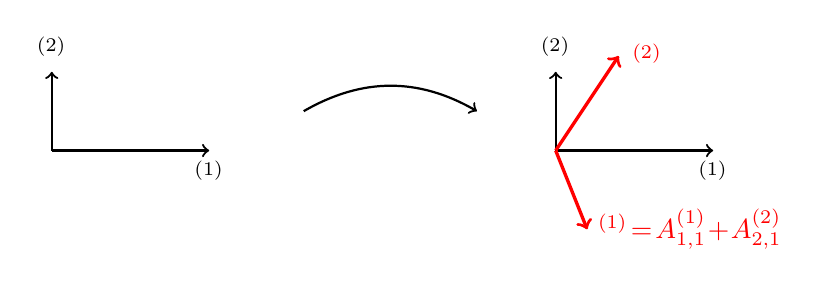
\begin{tikzpicture}[x=2cm]
			% LEFT: Standard basis vectors and unit square
			\begin{scope}
				\draw[->, thick] (0,0) -- (1,0) node[below] {$\vu^{(1)}$};
				\draw[->, thick] (0,0) -- (0,1) node[above] {$\vu^{(2)}$};
				%\draw[fill=gray!15] (0,0) -- (1,0) -- (1,1) -- (0,1) -- cycle;
				%\node at (0.5,0.5) {\small unit square};
				%\node at (0.5,-0.6) {standard basis};
			\end{scope}
			% RIGHT: Transformed basis vectors and parallelogram
			\begin{scope}[shift={(3.2,0)}]
				\draw[->, thick] (0,0) -- (1,0) node[below] {$\vv^{(1)}$};
				\draw[->, thick] (0,0) -- (0,1) node[above] {$\vv^{(2)}$};
				\coordinate (A) at (0.2,-1.0);
				\coordinate (B) at (0.4,1.2);
				\draw[->, very thick, red] (0,0) -- (A) node[below,right] {$\mA \vu^{(1)}\!=\!A_{1,1}\vv^{(1)}\!+\!A_{2,1}\vv^{(2)}$};
				\draw[->, very thick, red] (0,0) -- (B) node[right,xshift=1pt] {$\mA \vu^{(2)}$};
				%	\node[blue] at (0.25,1.25) {};
				%	\node at (0.8,-0.6) {transformed basis};
			\end{scope}
			% Arrow between plots
			\draw[->, thick] (1.6,0.5) to[bend left] node[midway, above] {$\mA$} (2.7,0.5);
		%	\draw[->, thick] (1.3,0.5) -- (2.4,0.5) node[midway, above] {$\mA$};
		\end{tikzpicture}
		\end{center}
		\caption{A matrix $\mA$ defines a \gls{linearmap} between two \glspl{vectorspace}. \label{fig_matrix_dict}} 
		\end{figure}
		See also: \gls{linearmap}, \gls{dataset}, \gls{linmodel}. },
	first={matrix},
	firstplural={matrices},
	type=math,
	plural={matrices},
	text={matrix}
}

\newglossaryentry{stratification}
{name={stratification},
 description={The process of splitting a \gls{dataset} into subsets, so called \glspl{stratum},
 according to some key attribute is called stratification\index{stratification} \cite{oecd2008glossary,Everitt2010,OxfordStatisticsDictionary}. 
 The goal is to ensure that a \gls{ml} method performs well for each \gls{stratum} 
defined by these attributes. For example, in a medical \gls{dataset},
  we may want to stratify a patient \gls{dataset} by age groups to ensure that an
  \gls{ml} model performs well across all age groups.  
 \begin{figure}[H]
 	\centering
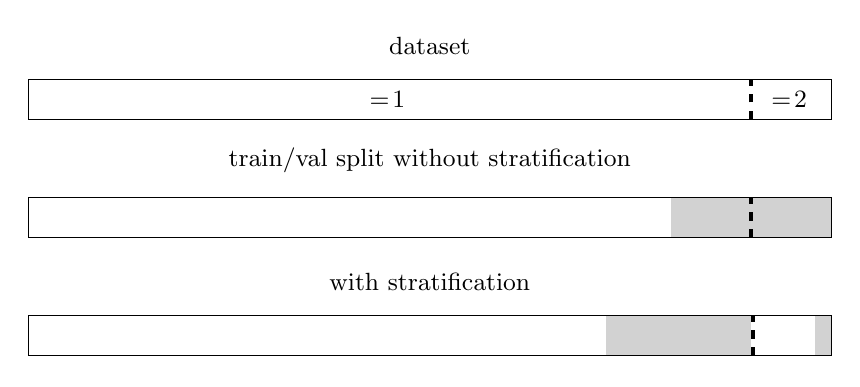
\begin{tikzpicture}[font=\small,x=1.7cm]
	% --- Parameters ---
	\def\cellw{6.0}     % total dataset width
	\def\cellh{0.5}     % height of one row
	\def\gap{1}       % vertical gap between rows
	\def\tfrac{0.8}     % train fraction
	\def\pA{0.9}        % proportion of stratum A (B = 1 - pA)
	% Column labels
	\node[anchor=south] at (0.5*\cellw, \cellh+0.2) {\gls{dataset}};
	\node[anchor=south] at ({0.5*\cellw}, {-(\cellh+\gap)+\cellh+0.2}) {train/val split without \gls{stratification}};
	\node[anchor=south] at (0.5*\cellw, {-2*(\cellh+\gap)+\cellh+0.2}) {with \gls{stratification}};
	% y-positions
	\pgfmathsetmacro{\yDataset}{0}
	\pgfmathsetmacro{\yNoStrat}{-(\cellh+\gap)}
	\pgfmathsetmacro{\yStrat}{-2*(\cellh+\gap)}
	% A/B border x (dataset coordinate)
	\pgfmathsetmacro{\xAB}{\pA*\cellw}
	\pgfmathsetmacro{\wA}{\pA*\cellw}
	\pgfmathsetmacro{\wB}{(1-\pA)*\cellw}
	% --- Row 1: DATASET (only A/B border) ---
	\draw (0,\yDataset) rectangle ++(\cellw,\cellh);
	\draw[dashed,  line width=0.5mm] (\xAB,\yDataset) -- ++(0,\cellh);
		% Labels for strata in Dataset row
	\node at (0.5*\wA, \yDataset+0.5*\cellh) {$\sensattr\!=\!1$};
	\node at ({\xAB+0.5*\wB}, {\yDataset+0.5*\cellh}) {$\sensattr\!=\!2$};
%	% --- Row 2: NO STRATIFICATION (shade right 20% as validation) ---
	\draw (0,\yNoStrat) rectangle ++(\cellw,\cellh);
	\pgfmathsetmacro{\xValStart}{\tfrac*\cellw}
	\pgfmathsetmacro{\valw}{(1-\tfrac)*\cellw}
	\fill[gray!35] (\xValStart,\yNoStrat) rectangle ++(\valw,\cellh);
%	\fill[gray!35] (\xValStart,\yNoStrat) rectangle ++({(1-\tfrac)*\cellw,\cellh});
%	% A/B border in dataset order only
	\draw[dashed,  line width=0.5mm] (\xAB,\yNoStrat) -- ++(0,\cellh);
	% --- Row 3: STRATIFIED (shade val inside each stratum A and B) ---
	\draw (0,\yStrat) rectangle ++(\cellw,\cellh);
	% A/B border at x = pA * cellw
	\pgfmathsetmacro{\xAB}{\pA*\cellw}
	\draw[dashed, line width=1mm] (\xAB,\yStrat) -- ++(0,\cellh);
	% widths of strata A and B
	% --- Validation area within A (right (1-tfrac) part of A) ---
	\pgfmathsetmacro{\xAVal}{\tfrac*\wA}              % start inside A (A begins at x=0)
	\pgfmathsetmacro{\wAVal}{(1-\tfrac)*\wA}          % width of A's validation
	\fill[gray!35] (\xAVal,\yStrat) rectangle ++(\wAVal,\cellh);
	% --- Validation area within B (right (1-tfrac) part of B) ---
	\pgfmathsetmacro{\xBVal}{\xAB + \tfrac*\wB}       % start inside B
	\pgfmathsetmacro{\wBVal}{(1-\tfrac)*\wB}          % width of B's validation
	\fill[gray!35] (\xBVal,\yStrat) rectangle ++(\wBVal,\cellh);
\end{tikzpicture}
 	\caption{Stratification ensures that both the \gls{trainset} and the \gls{valset} 
	(shaded grey) have similar 
 		distributions of a binary key attribute $\sensattr$.}
 \end{figure}
  When splitting a \gls{dataset} into a \gls{trainset} and a \gls{valset}, 
  stratification ensures that both sets have similar distributions of the key attribute. 
  Without stratification, using a small \gls{valset} may underrepresent or 
  even completely miss \glspl{datapoint} with a rare attribute, leading to misleading 
  performance estimates.\\ 
  See also: \gls{validation}, \gls{kfoldcv}, \gls{stratum}.},
  text={stratification},
  first={stratification},
  plural={stratifications}%
}

\newglossaryentry{stratum}
{name={stratum},
	description={
	A\index{stratum} stratum is a subset of \glspl{datapoint} that all 
	possess a shared property (which could be a \gls{feature} or a \gls{label}). 
	For example, in a weather \gls{dataset}, all measurements from the same 
	\gls{fmi} weather station form one stratum.\\[0.5em]
	\begin{center}
\textbf{Example (CSV snippet):}\\
  {\ttfamily
  time,station,value,units\\
  2023-06-01 12:00,Helsinki,18.2,degC\\
  2023-06-01 13:00,Helsinki,18.5,degC\\
  2023-06-01 14:00,Helsinki,19.0,degC\\
  2023-06-01 12:00,Oulu,12.1,degC\\
  2023-06-01 13:00,Oulu,12.4,degC\\
  2023-06-01 14:00,Oulu,12.7,degC\\
  2023-06-01 12:00,Tampere,15.3,degC\\
  2023-06-01 13:00,Tampere,15.6,degC\\
  2023-06-01 14:00,Tampere,16.0,degC
  }
	\end{center} 
	Here, the rows for each station (\texttt{Helsinki}, \texttt{Oulu}, \texttt{Tampere}) 
	represent different strata.\\ 
	See also: \gls{stratification}, \gls{dataset}, \gls{datapoint}.},
  first={stratum},
  firstplural={strata},
 plural={strata}, 
 text={stratum}
}


\newglossaryentry{det}
{name={determinant},
	description={The\index{determinant} determinant $\det\,(\mA)$ of a square \gls{matrix} 
		$\mA =\linebreak \big( \va^{(1)},\,\ldots,\,\va^{(\nrfeatures)} \big) \in \mathbb{R}^{\nrfeatures \times \nrfeatures}$ is a 
		\gls{function} of its columns $\va^{(1)},\,\ldots,\,\va^{(\nrfeatures)} \in \mathbb{R}^{\nrfeatures}$, i.e., it satisfies 
		the following properties \cite{DirschmidHansJorg1996TuF}:
		\begin{itemize}
			\item Normalized: $$\det\,(\mI) = 1$$ 
			\item Multilinear: \begin{align} \nonumber \det \big(\va^{(1)},\,\ldots,\,\alpha\vu+ \beta \vv,\,\ldots,\,\va^{(\nrfeatures)} \big) & = \alpha\det \big(\va^{(1)},\,\ldots,\,\vu,\,\ldots,\,\va^{(\nrfeatures)} \big) \\ 
			& +\beta\det \big(\va^{(1)},\,\ldots,\,\vv,\,\ldots,\,\va^{(\nrfeatures)} \big) \nonumber
			\end{align}
			\item Antisymmetric: $$\det \big(\ldots,\,\va^{(\featureidx)}, \,\ldots, \,\va^{(\featureidx')},\,\ldots \big) = - \det \big(\ldots,\,\va^{(\featureidx')}, \,\ldots, \,\va^{(\featureidx)},\,\ldots \big).$$ 
		\end{itemize} 
		We can interpret a \gls{matrix} $\mA$ as a linear transformation on $\mathbb{R}^{\nrfeatures}$.
		The determinant $\det\,(\mA)$ characterizes how volumes in $\mathbb{R}^\nrfeatures$ (and their orientation) 
		are altered by this transformation (see Fig. \ref{fig_det_dict}) \cite{GolubVanLoanBook}, \cite{Strang2007}. 
 		In particular, $\det\,(\mA) > 0$ preserves orientation, $\det\,(\mA) < 0$ reverses orientation, 
 		and $\det\,(\mA) = 0$ collapses volume entirely, indicating that $\mA$ is non-invertible. 
 		The determinant also satisfies $\det\,(\mA \mB) = \det\,(\mA) \cdot \det\,(\mB)$, and if $\mA$ is 
 		diagonalizable with \glspl{eigenvalue} $\eigval{1}, \,\ldots, \,\eigval{\nrfeatures}$, then 
		$\det\,(\mA) = \prod_{\featureidx=1}^{\nrfeatures} \eigval{\featureidx}$ \cite{HornMatAnalysis}.
    		For the special cases $\nrfeatures=2$ (i.e., two-dimensional or 2-D) and $\nrfeatures=3$ (i.e., three-dimensional or 3-D), 
		the determinant can be interpreted as an oriented area or volume spanned by the column \glspl{vector} of $\mA$.
    		\begin{figure}[H]
    			\begin{center}
    			\begin{tikzpicture}[x=2cm]
			% LEFT: Standard basis vectors and unit square
			\begin{scope}
			\draw[->, thick] (0,0) -- (1,0) node[below right] {$\vx$};
			\draw[->, thick] (0,0) -- (0,1) node[above left] {$\vy$};
			%\draw[fill=gray!15] (0,0) -- (1,0) -- (1,1) -- (0,1) -- cycle;
			%\node at (0.5,0.5) {\small unit square};
			%\node at (0.5,-0.6) {standard basis};
			\end{scope}
			% RIGHT: Transformed basis vectors and parallelogram
			\begin{scope}[shift={(2.8,0)}]
			\coordinate (A) at (1.5,0.5);
			\coordinate (B) at (-0.2,1.2);
			\draw[->, very thick, red] (0,0) -- (A) node[below right] {$\mA \vx$};
			\draw[->, very thick, red] (0,0) -- (B) node[above left] {$\mA \vy$};
			\draw[fill=red!20, opacity=0.6] (0,0) -- (A) -- ($(A)+(B)$) -- (B) -- cycle;
			\draw[dashed] (A) -- ($(A)+(B)$);
			\draw[dashed] (B) -- ($(A)+(B)$);
			\node at (0.8,0.6) {\small $\det\,(\mA)$};
			% Orientation arc
			\draw[->, thick, blue] (0.4,0.0) arc[start angle=0, end angle=35, radius=0.6];
			%	\node[blue] at (0.25,1.25) {};
			%	\node at (0.8,-0.6) {transformed basis};
			\end{scope}
			% Arrow between plots
			\draw[->, thick] (1.3,0.5) -- (2.4,0.5) node[midway, above] {$\mA$};
			\end{tikzpicture}
			\end{center}
			\caption{We can interpret a square \gls{matrix} $\mA$ as a linear transformation of $\mathbb{R}^{\nrfeatures}$ 
				into itself. The determinant $\det\,(\mA)$ characterizes how this transformation alters an oriented volume.
				\label{fig_det_dict}}
		\end{figure}
		See also: \gls{eigenvalue}, \gls{inverse}.},
	first={determinant},
	type=math,
	text={determinant}
}

\newglossaryentry{hessian}
{name={Hessian},
 	description={Consider\index{Hessian} a \gls{function} 
	$f: \mathbb{R}^{\nrfeatures} \to \mathbb{R}$ for which the second-order 
	partial derivatives exist at $\featurevec'$. Then, the Hessian $\nabla^2 f(\featurevec')$ 
	of $f$ at $\featurevec$ is defined as the \gls{matrix} of second-order 
	partial derivatives of $f$ at $\featurevec'$, 
$$\nabla^{2} f(\featurevec') \;=\;
\begin{pmatrix}
\frac{\partial^{2} f}{\partial \feature_{1}^{2}}
& \frac{\partial^{2} f}{\partial \feature_{1}\, \partial \feature_{2}}
& \cdots
& \frac{\partial^{2} f}{\partial \feature_{1}\, \partial \feature_{\nrfeatures}} \\
\frac{\partial^{2} f}{\partial \feature_{2}\, \partial \feature_{1}}
& \frac{\partial^{2} f}{\partial \feature_{2}^{2}}
& \cdots
& \frac{\partial^{2} f}{\partial \feature_{2}\, \partial \feature_{\nrfeatures}} \\
\vdots & \vdots & \ddots & \vdots \\[1.2ex]
\frac{\partial^{2} f}{\partial \feature_{\nrfeatures}\, \partial \feature_{1}}
& \frac{\partial^{2} f}{\partial \feature_{\nrfeatures}\, \partial \feature_{2}}
& \cdots
& \frac{\partial^{2} f}{\partial \feature_{\nrfeatures}^{2}}
\end{pmatrix}.$$
If the second-order partial derivatives are \gls{continuous} in a \gls{neighborhood} around $\featurevec'$, then the Hessian is a symmetric \gls{matrix}, i.e.,
$\frac{\partial^{2} f}{\partial \feature_{\featureidx}\, \partial \feature_{\featureidx'}} = 
\frac{\partial^{2} f}{\partial \feature_{\featureidx'}\, \partial \feature_{\featureidx}}$ for all 
$\featureidx, \featureidx'$ \cite{RudinBookPrinciplesMatheAnalysis}. If additionally $f$ 
is \gls{convex}, then the Hessian is a \gls{psd} \gls{matrix} \cite{BoydConvexBook}.
	\begin{figure}[H]
	\begin{center}
	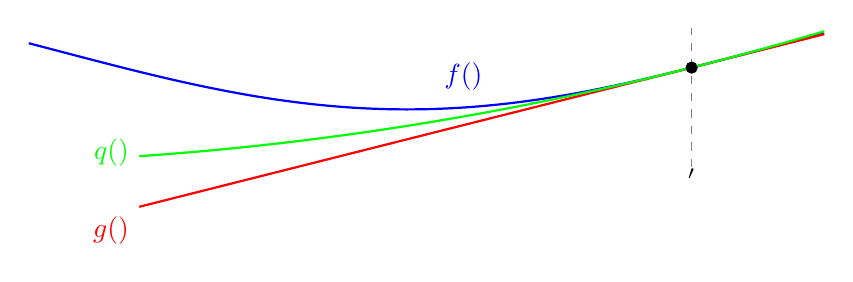
\begin{tikzpicture}[x=0.5cm]
		\begin{axis}[
			hide axis,
			xmin=3, xmax=6,
			ymin=0, ymax=6,
			domain=0:6,
			samples=100,
			width=10cm,
			height=6cm,
			clip=false
			]
		% Original nonlinear function h(x)
			\addplot[blue, thick, domain=3:6.6] {2 + sin(deg(x))} 
			node[pos=0.5, above right, yshift=3pt] {$f(\featurevec)$};
		% Tangent line as local linear approximation at x = 3
		% h(3) = 2 + sin(3), h'(3) = cos(3)
			\addplot[red, thick, domain=3.5:6.6] 
			{2 + sin(deg(6)) + cos(deg(6))*(x - 6)}
			node[pos=0, below left] {$g(\featurevec)$};
                %%%%%%%%%%%%%%%%%%%%%%%%%%%%%%%%%%%%%%%%%%%%%%%%
                \addplot[green, thick, domain=3.5:6.6]
                {2 + sin(deg(6)) + cos(deg(6))*(x - 6) - 0.5*sin(deg(6))*(x - 6)^2}
			node[pos=0, below left, yshift=10pt] {$q(\featurevec)$};
                %%%%%%%%%%%%%%%%%%%%%%%%%%%%%%%%%%%%%%%%%%%%%%%%
		% Mark point of approximation
			\addplot[mark=*] coordinates {(6, {2 + sin(deg(6))})};
			    % Vertical dashed line (ruler) at x = 3
			\addplot[dashed, gray] coordinates {(6,0) (6,2.4)};
			\node at (axis cs:6, -0.2) {$\featurevec'$};
			    % Plot the two points
			    % Coordinates of the two points
			\pgfmathsetmacro{\xA}{-1.5}
			\pgfmathsetmacro{\xB}{3}
			\pgfmathsetmacro{\yA}{2 + sin(deg(\xA))}
			\pgfmathsetmacro{\yB}{2 + sin(deg(\xB))}
		\end{axis}
		\vspace*{-10mm}
	\end{tikzpicture}
		\vspace*{-5mm}
	\end{center}
	\caption{
		A \gls{function} $f(\featurevec)$ that is sufficiently \gls{smooth} at a 
		point $\featurevec'$ can be locally approximated by 
		a \gls{quadfunc} $q(\featurevec)$ which allows for a more accurate approximation 
		compared to a linear \gls{function} $g(\featurevec)$. \label{fig_quadapprox_hessian_dict}}
\end{figure}
		The Hessian $\nabla^2 f(\featurevec')$ can be used to compute a \gls{quadfunc} 
		$$q(\featurevec) = (1/2) (\featurevec- \featurevec')^{T} \underbrace{\nabla^2 f(\featurevec')}_{\text{Hessian}} 
		(\featurevec- \featurevec') +  (\featurevec- \featurevec')^{T} \underbrace{\nabla f(\featurevec')}_{\text{gradient}} 
		+ f(\featurevec')$$
		that approximates $f$ locally around $\featurevec'$. 
        		\\
		See also: \gls{differentiable}, \gls{matrix}, \gls{function}, \gls{quadfunc}. }, 
	first={Hessian},
	type=math,
	text={Hessian}
}

\newglossaryentry{continuous}
{name={continuous}, 
description={A \gls{function}\index{continuous} $f: \mathbb{R}^{\nrfeatures} \to \mathbb{R}$ is 
	 continuous at a point $\featurevec' \in \mathbb{R}^{\nrfeatures}$ if for 
	 every $\epsilon > 0$ there is a $\delta > 0$ such that for all 
	 $\featurevec \in \mathbb{R}^{\nrfeatures}$ with $\normgeneric{\featurevec - \featurevec'}{2} < \delta$, 
	 it holds that $|f(\featurevec) - f(\featurevec')| < \epsilon$ \cite{RudinBookPrinciplesMatheAnalysis}. 
	 In other words, we can make $f(\featurevec)$ arbitrarily close to $f(\featurevec')$ 
	 by choosing $\featurevec$ sufficiently close to $\featurevec'$. If $f$ is continuous 
	 at every point $\featurevec' \in \mathbb{R}^{\nrfeatures}$, then $f$ is said to be 
	 continuous on $\mathbb{R}^{\nrfeatures}$. The notion of a continuous 
	 \gls{function} can be naturally extended to \glspl{function} between general \gls{metric} 
	 spaces \cite{RudinBookPrinciplesMatheAnalysis}.\\
		See also: \gls{euclidspace}, \gls{metric}.},
	first={continuous},
	type=math,
	text={continuous}
}

\newglossaryentry{linearmap}
{name={linear map}, plural={linear maps}, 
	description={A\index{linear map} linear \gls{map} $f: \mathbb{R}^n \rightarrow \mathbb{R}^m$ is a \gls{function} that satisfies additivity, i.e.,
		$f(\vx + \vy) = f(\vx) + f(\vy)$, and homogeneity, i.e.,
		$f(c\vx) = c f(\vx)$, for all \glspl{vector} $\vx, \vy \in \mathbb{R}^n$ and scalars $c \in \mathbb{R}$. 
		In particular, $f(\mathbf{0}) = \mathbf{0}$. Any linear \gls{map} can be represented as a \gls{matrix} 
		multiplication $f(\vx) = \mA \vx$ for some \gls{matrix} $\mA \in \mathbb{R}^{m \times n}$. 
		The collection of real-valued linear \glspl{map} for a given dimension $n$ constitute a \gls{linmodel}, 
		which is used in many \gls{ml} methods.
		\\
		See also: \gls{map}, \gls{function}, \gls{vector}, \gls{matrix}, \gls{linmodel}, \gls{ml}.},
	first={linear map},
	text={linear map}
}

\newglossaryentry{vector}
{name={vector},
	description={A\index{vector} vector is an element of a \gls{vectorspace}. 
		In the context of \gls{ml}, a particularly important example of a \gls{vectorspace} 
		is the \gls{euclidspace} $\mathbb{R}^{\nrfeatures}$, where $\nrfeatures \in \mathbb{N}$ 
		is the (finite) dimension of the space. A vector $\vx \in \mathbb{R}^{\nrfeatures}$ 
		can be represented as a list or one-dimensional (1-D) array of real numbers, i.e., 
		$x_1, \,\ldots, \,x_{\nrfeatures}$ with $x_\featureidx \in \mathbb{R}$ for 
		$\featureidx = 1, \,\ldots, \,\nrfeatures$. The value $x_\featureidx$ is the $\featureidx$th 
		entry of the vector $\vx$. It can also be useful to view a vector $\vx \in \mathbb{R}^{\nrfeatures}$ 
		as a \gls{function} that maps each index $\featureidx \in \{1, \,\ldots, \,\nrfeatures\}$ 
		to a value $x_\featureidx \in \mathbb{R}$, i.e., $\vx: \featureidx \mapsto x_\featureidx$. 
		This perspective is particularly useful for the study of \glspl{kernelmethod}. See Fig. 
		\ref{fig:vector-function-dual_dict} for the two views of a vector.
		\begin{figure}[H]
			% Left: Stem plot
			\begin{minipage}[c]{0.48\textwidth}
				\centering 
				2, --1, 3, 0, --2, 1
				\begin{minipage}{\textwidth}
				\vspace{5ex}
				\centering
				{\selectfont (a)}
				\end{minipage}
			\end{minipage}
			\hfill
			% Right: Column vector
			\begin{minipage}{0.48\textwidth}
			\centering
			\begin{tikzpicture}
			\begin{axis}[
    				width=6.5cm,
    				height=5cm,
    				title={},
    				xlabel={index $\featureidx$},
    				ylabel={$x_\featureidx$},
   		 		ymin=-3.5, ymax=3.5,
    				xmin=0.5, xmax=6.5,
   	 			xtick={1,2,3,4,5,6},
    				ytick={-3,-2,-1,0,1,2,3},
    				axis x line=bottom,        % <-- horizontal axis at y=0
    				axis y line=left,          % <-- vertical axis on the left
    				grid=both,
    				major grid style={dotted, gray!60},
    				enlargelimits=0.1
			]
			\addplot+[ycomb, thick, mark=*]
    			coordinates {
        				(1,2)
        				(2,-1)
       	 			(3,3)
        				(4,0)
        				(5,-2)
        				(6,1)
    			};
			\end{axis}
			\node at (2,-2.5) {(b)};
			\end{tikzpicture}
			\end{minipage}
			\caption{Two equivalent views of a vector $\vx= \big( 2, -1, 3, 0, -2, 1 \big)^{T} \in \mathbb{R}^{6}$.
			(a) As a numeric array. (b) As a \gls{map} $\featureidx \mapsto x_\featureidx$.}
			\label{fig:vector-function-dual_dict}
		\end{figure}
		See also: \gls{vectorspace}, \gls{euclidspace}, \gls{linearmap}.},
	first={vector},
	firstplural={vectors},
	type=math,
	plural={vectors},
	text={vector}
}


\newglossaryentry{vectorspace}
{name={vector space},
	description={A\index{vector space} \gls{vector} space $\mathcal{V}$ (also called linear space) 
		is a collection of elements, called \glspl{vector}, along with the following two operations 
		(see also Fig. \ref{fig:vector-ops_dict}): 
    		1) addition (denoted by $\vv+\vw$) of two \glspl{vector} $\vv,\vw$; and 2) multiplication 
		(denoted by $c \,\cdot \,\vv$) of a \gls{vector} $\vv$ with a scalar $c$ that belongs to some 
		number field (with a typical choice for this field being $\mathbb{R}$). The defining 
		property of a \gls{vector} space is that it is closed under two specific operations. First, 
		if $\vv, \vw \in \mathcal{V}$, then $\vv + \vw \in \mathcal{V}$. Second, if $\vv \in \mathcal{V}$ 
		and $c \in \mathbb{R}$, then $c \vv \in \mathcal{V}$.
		\begin{figure}[H]
		\centering
			\begin{tikzpicture}[>=Stealth, scale=1.2]
			% Coordinates
  			\coordinate (O) at (0,0);            % Origin
  			\coordinate (V) at (2,1.5);          % vector v
  			\coordinate (W) at (1,3);            % vector w
  			\coordinate (VplusW) at (3,4.5);     % v + w
  			\coordinate (HalfV) at (1,0.75);     % 0.5 * v
  			\draw[->, thick, blue] (O) -- (V) node[pos=1, right] {$\vv$};
  			\draw[->, thick, red] (O) -- (W) node[pos=1, left] {$\vw$};
  			\draw[->, thick, purple] (O) -- (VplusW) node[pos=0.99, above right] {$\vv+\vw$};
  			\draw[dashed, red] (V) -- (VplusW);
  			\draw[dashed, blue] (W) -- (VplusW);
  			\draw[->, thick, orange] (O) -- (HalfV) node[midway, right] {$ \alpha \vv$};
			% Filled dots
  			\filldraw[black] (O) circle (2pt) node[below left] {$\mathbf{0}$};  % origin
  			\filldraw[blue] (V) circle (2pt);         % v
  			\filldraw[red] (W) circle (2pt);          % w
  			\filldraw[purple] (VplusW) circle (2pt);  % v + w
  			\filldraw[orange] (HalfV) circle (2pt);   % 0.5v
			\end{tikzpicture}
			\caption{A \gls{vector} space $\mathcal{V}$ is a collection of \glspl{vector} such that 
			scaling and adding them always yields another \gls{vector} in $\mathcal{V}$.}
			%In \gls{ml}, we use vector spaces to represent \glspl{rv}, \glspl{datapoint} 
			%(or their \glspl{featurevec}) as well as invariances (or symmetries) of \glspl{model}.}
			\label{fig:vector-ops_dict}
		\end{figure}
		A common example of a \gls{vector} space is the \gls{euclidspace} $\mathbb{R}^n$, which is 
		widely used in \gls{ml} to represent \glspl{dataset}. We can also use $\mathbb{R}^n$ 
		to represent, either exactly or approximately, the \gls{hypospace} used by an \gls{ml} method.  
		Another example of a \gls{vector} space, which is naturally associated with every \gls{probspace} 
		$\big(\samplespace,\eventspace,\prob{\cdot} \big)$, is the collection of all 
		real-valued \glspl{rv} $x: \samplespace \rightarrow \mathbb{R}$ \cite{RudinBook}, \cite{folland1999real}.  
		\\
		See also: \gls{vector}, \gls{euclidspace}, \gls{linmodel}, \gls{linearmap}.},
	first={vector space},
	type=math,
	text={vector space}
}


\newglossaryentry{stochastic}
{name={stochastic},
	description={We refer to a \index{stochastic} method as stochastic if it involves a 
		random component or is governed by probabilistic laws. \Gls{ml} methods use randomness 
		to reduce computational complexity (e.g., see \gls{stochGD}) or 
		to capture \gls{uncertainty} in \glspl{probmodel}.
		\\
		See also: \gls{stochGD}, \gls{uncertainty}, \gls{probmodel}.},
	first={stochastic},
	text={stochastic}
}

\newglossaryentry{stochproc}
{name={stochastic process},
	description={A \gls{stochastic} process\index{stochastic process} is a collection of 
		\glspl{rv} defined on a common \gls{probspace} and indexed by some set 
		$\mathcal{I}$ \cite{GrayProbBook}, \cite{papoulis}, \cite{Brockwell91}. The index set 
		$\mathcal{I}$ typically represents time or space, allowing us to represent 
		random phenomena that evolve across time or spatial dimensions—for example, 
		sensor noise or financial time series. \Gls{stochastic} processes are not limited 
		to temporal or spatial settings. For instance, random \glspl{graph} such as 
		the \gls{ergraph} or the \gls{sbm} can also be viewed as \gls{stochastic} processes. 
		Here, the index set $\mathcal{I}$ consists of node pairs that index \glspl{rv} whose values 
		encode the presence or weight of an edge between two nodes. Moreover, \gls{stochastic} 
		processes naturally arise in the analysis of \glspl{stochalgorithm}, 
		such as \gls{stochGD}, which construct a sequence of \glspl{rv}. 
		\\
		See also:  \gls{rv}, \gls{sbm}, \gls{stochGD}, \gls{uncertainty}, \gls{probmodel}.},
	first={stochastic process},
	firstplural={stochastic processes},
	type=math, 
	plural={stochastic processes},
	text={stochastic process}
}

\newglossaryentry{characteristicfunc}
{name={characteristic function},
	description={The characteristic \gls{function}\index{characteristic function} 
		of a real-valued \gls{rv} $x$ is the \gls{function} \cite[Sec. 26]{BillingsleyProbMeasure}
		$$ \phi_{x}(t) \defeq \expect { \exp\,(j t x) } \mbox{ with } j = \sqrt{-1}.$$
	 	The characteristic \gls{function} uniquely determines the \gls{probdist} of $x$. 
		\\
		See also: \gls{rv}, \gls{probdist}.},
	first={characteristic function},
	firstplural={characteristic functions}, 
	type=math, 
	plural={characteristic functions},
	text={characteristic function}
}

\newglossaryentry{entropy}
{name={entropy},
	description={Entropy\index{entropy} quantifies the \gls{uncertainty} or unpredictability associated with a \gls{rv} \cite{coverthomas}. 
		For a discrete \gls{rv} $x$ taking on values in a finite set $\mathcal{S} = \{x_1, \,\ldots, \,x_n\}$ with 
		a \gls{probability} mass \gls{function} $p_i \defeq \prob{x = x_i}$, the entropy is defined as
		\[
		H(x) \defeq -\sum_{i=1}^n p_i \log p_i.
		\]
		Entropy is maximized when all outcomes are equally likely, and minimized (i.e., zero) 
		when the outcome is deterministic. A \gls{generalization} of the concept of entropy for continuous 
		\glspl{rv} is \gls{diffentropy}. 
		\\
		See also: \gls{uncertainty}, \gls{probmodel}.},
	first={entropy},
	text={entropy}
}

\newglossaryentry{diffentropy}
{name={differential entropy},
	description={For\index{differential entropy} a real-valued \gls{rv} $\featurevec \in \mathbb{R}^{\nrfeatures}$ 
		with a \gls{pdf} $p(x)$, the differential \gls{entropy} is defined as \cite{coverthomas}
		\[
		h(\featurevec) \defeq - \int p(\featurevec) \log p(\featurevec) \, d\featurevec.
		\]
		Differential \gls{entropy} can be negative and lacks some properties of \gls{entropy} for 
		discrete-valued \glspl{rv}, such as invariance under a change of variables \cite{coverthomas}. 
		Among all \glspl{rv} with a given \gls{mean} $\meanvecgeneric$ and \gls{covmtx} $\covmtxgeneric$, 
		$h(\featurevec)$ is maximized by $\featurevec \sim \mvnormal{\meanvecgeneric}{\covmtxgeneric}$. 
		\\
		See also: \gls{uncertainty}, \gls{probmodel}.},
	first={differential entropy},
	text={differential entropy}
}

\newglossaryentry{minimum}
{name={minimum},
	description={Given a set of real numbers, the minimum\index{minimum} is the smallest of those numbers.
		Note that for some sets, such as the set of negative real numbers, the minimum does not exist.},
	firstplural={minima}, 
 	plural={minima},
	first={minimum},
	text={minimum}
}


\newglossaryentry{co-domain}
{name={co-domain}, 
	description={The co-domain\index{co-domain} of a \gls{function} 
	$f: \mathcal{U} \rightarrow \mathcal{V}$ is the set $\mathcal{V}$ 
		into which $f$ maps elements of its domain $\mathcal{U}$.  
		\\
		See also: \gls{function}, \gls{domain}, \gls{map}.},
	first={co-domain},
	firstplural={co-domains}, 
	type=math, 
	plural={co-domains},
	text={co-domain}
}

\newglossaryentry{domain}
{name={domain}, 
	description={The domain\index{domain} of a \gls{function} 
	$f: \mathcal{U} \rightarrow \mathcal{V}$ is the set $\mathcal{U}$ 
		from which $f$ takes its inputs.  
		\\
		See also: \gls{function}, \gls{co-domain}, \gls{map}.},
	first={domain},
	firstplural={domains}, 
	type=math, 
	plural={domains},
	text={domain}
}	
	

\newglossaryentry{function}
{name={function}, 
	description={A function\index{function} between two sets $\mathcal{U}$ and $\mathcal{V}$ assigns  
		each element $u \in \mathcal{U}$ exactly one element $f(u) \in \mathcal{V}$ \cite{RudinBookPrinciplesMatheAnalysis}.
		We write this as $$f: \mathcal{U} \rightarrow \mathcal{V}: u \mapsto f(u)$$ 
		where $\mathcal{U}$ is the domain and $\mathcal{V}$ the co-domain of $f$. 
		That is, a function $f$ defines a unique output $f(u) \in \mathcal{V}$ for every 
		input $u \in \mathcal{U}$ (see Fig. \ref{fig_function_dict}).
		\begin{figure}[H]
			\centering
			\begin{tikzpicture}[>=stealth, node distance=1.2cm and 2.5cm]
				\tikzset{dot/.style={circle, fill=black, inner sep=1.2pt}}
				\node (A) [dot, label=left:$a$] {};
				\node (B) [dot, below=of A, label=left:$b$] {};
				\node (C) [dot, below=of B, label=left:$c$] {};
				\node (1) [dot, right=4cm of A, label=right:$\star$] {};
				\node (2) [dot, below=of 1, label=right:$\circ$] {};
				\node (3) [dot, below=of 2, label=right:$\otimes$] {};
				\node[draw=blue!70, thick, ellipse, inner sep=0.5cm, fit=(A)(B)(C), label=above:$\mathcal{U}$] {};
				\node[draw=green!70!black, thick, ellipse, inner sep=0.5cm, fit=(1)(2)(3), label=above:$\mathcal{V}$] {};
				\draw[->] (A) -- (2);
				\draw[->] (B) -- (1);
				\draw[->] (C) -- (2);
			\end{tikzpicture}
			\caption{A function \( f \colon \mathcal{U} \to \mathcal{V} \) mapping each element 
			of the domain $\mathcal{U} =  \{a,b,c\}$ to exactly one element of 
				the co-domain $\mathcal{V} = \{\star,\circ,\otimes\}$. \label{fig_function_dict}}
		\end{figure} },
	first={function},
	firstplural={functions}, 
	type=math, 
	plural={functions},
	text={function}
}


\newglossaryentry{map}
{name={map}, 
	description={We\index{map} use the term map as a synonym for \gls{function}.
		\\
		See also: \gls{function}.},
	first={map},
	firstplural={maps},	
	type=math, 
	plural={maps},
	text={map}
}


\newglossaryentry{attention}
{name={attention}, 
	description={Some \gls{ml} applications\index{attention} involve \glspl{datapoint} 
	composed of smaller units, referred to as \glspl{token}. For example, a sentence 
	consists of words, an image of pixel patches, and a network of nodes. In general, 
	the \glspl{token} that constitute a single \gls{datapoint} are not independent 
	of one another. Instead, each \gls{token} of a \gls{datapoint} depends (or pays attention) 
	to specific other \glspl{token}. \Glspl{probmodel} provide a principled framework for 
	representing and analyzing such dependencies \cite{Blei2003}. Attention mechanisms use 
	a more direct approach without explicit reference to a \gls{probmodel}. The idea is to 
		represent the relationship between two tokens $\nodeidx$ and $\nodeidx'$ using a parameterized \gls{function} $f^{(\weights)}(\nodeidx,\nodeidx')$, 
		where the \glspl{parameter} $\weights$ are learned via a variant of \gls{erm}. 
		Practical attention mechanisms differ in their precise choice of attention \gls{model} $f^{(\weights)}(\nodeidx,\nodeidx')$ 
		as well as in the precise \gls{erm} variant used to learn the \glspl{parameter} $\weights$. One widely used family of attention mechanisms 
		defines the parameters $\weights$ in terms of two \glspl{vector} associated with each token $\nodeidx$, i.e.,
		a query \gls{vector} $\vq^{(\nodeidx)}$ and a key \gls{vector} $\vk^{(\nodeidx')}$. For a given token $\nodeidx$ 
		with query $\vq^{(\nodeidx)}$, and another token $\nodeidx'$ with key $\vk^{(\nodeidx')}$, the quantity 
		$\big( \vq^{(\nodeidx)} \big)^{\top} \vk^{(\nodeidx')}$ quantifies the extent to which token $\nodeidx$ attends 
		to (or depends on) token $\nodeidx'$ (see Fig. \ref{fig_attention_dict}).
		\begin{figure}[H]
			\centering
			\begin{tikzpicture}[>=stealth, node distance=0.2cm and 0.2cm,
			every node/.style={inner sep=2pt, font=\large}, baseline]
			% Words (sentence: All human beings are born free and equal.)
			\node (w1) [draw, fill=gray!10, rounded corners] {All};
			\node (w2) [draw, fill=gray!10, right=of w1, rounded corners] {human};
			\node (w3) [draw, fill=gray!10, right=of w2, rounded corners] {beings};
			\node (w4) [draw, fill=gray!10, right=of w3, rounded corners] {are};
			\node (w5) [draw, fill=gray!10, right=of w4, rounded corners] {born};
			\node (w6) [draw, fill=gray!10, right=of w5, rounded corners] {free};
			\node (w7) [draw, fill=gray!10, right=of w6, rounded corners] {and};
			\node (w8) [draw, fill=blue!20, right=of w7, rounded corners] {equal};
			% Label "i" below the word "equal"
   	   		\node[font=\footnotesize, below=0.15cm of w8, align=center] (labeli) {$\nodeidx$ \\ $\vq^{(\nodeidx)},\ \vk^{(\nodeidx)}$};
			\node[font=\footnotesize, below=0.15cm of w1, align=center] (labelii) {$\nodeidx'$ \\ $\vq^{(\nodeidx')},\ \vk^{(\nodeidx')}$};
			% Dummy node above for routing attention arrows
	  		\node (eqTop) [above=1.8cm of w8] {};
	 		% Arrows from "equal" to earlier words (drawn above)
	 		\draw[->, thick, opacity=0.3] (w8.north) .. controls +(up:1.0cm) and +(up:1.0cm) .. (w6.north); % to "free"
	 		\draw[->, thick, opacity=0.3] (w8.north) .. controls +(up:1.2cm) and +(up:1.0cm) .. (w5.north); % to "born"
			\draw[->, thick, opacity=1]  (w8.north)  .. controls +(up:1.8cm) and +(up:1.0cm) ..  node[midway, text=black, above] {$f^{(\weights)}(\nodeidx,\nodeidx')$}  (w1.north); % to "All"
			\end{tikzpicture}
			\caption{Attention mechanisms learn a parameterized \gls{function} $f^{(\weights)}(\nodeidx,\nodeidx')$ to measure 
				how much token $\nodeidx$ attends to token $\nodeidx'$. One widely used construction of $f^{(\weights)}(\nodeidx,\nodeidx')$ 
				uses query and key \glspl{vector}, denoted by $\vq^{(\nodeidx)}$ and $\vk^{(\nodeidx)}$, assigned to each 
				token $\nodeidx$ \cite{vaswani2017attention}. \label{fig_attention_dict}}
		\end{figure}
		See also: \gls{function}, \gls{nlp}, \gls{token}.},
	first={attention},
	text={attention}
}

\newglossaryentry{transformer}
{name={transformer},
 description={In the context of \gls{ml}, the term transformer\index{transformer} 
 	refers to an \glspl{ann} that uses some form of \gls{attention} mechanism 
 	to capture dependencies among \glspl{token} \cite{vaswani2017attention}. 
 	The \gls{attention} mechansim is what sets transformers apart from 
	previous \glspl{model} used for sequential \gls{data} such as \glspl{rnn}. 
	A transformer \gls{ann} often combines several \gls{attention} \glspl{layer} 
	that are combined via more traditional \gls{layer} architectures. \\ 
	See also: \gls{nlp}, \gls{attention}.
  }, 
 first = {transformer}, 
 text={transformer},
 firstplural={transformers}, 
 plural = {transformers}
}

\newglossaryentry{rnn}
{name={recurrent neural network (RNN)},
 description={A \index{recurrent neural network (RNN)} RNN 
  is a specific type of \gls{ann} that is designed for processing 
    \gls{data} that consists of a sequence of \glspl{token}. 
	An RNN maintains an internal hidden state that is updated recurrently 
	as new \glspl{token} are processed. This recurrent dependence allows 
	information to propagate across time steps, making RNNs suitable for 
	tasks such as speech recognition, language modeling, or time series prediction. 
    However, their inherently sequential computation limits parallelization and 
	is challenging for \glspl{gdmethod}. Variants like the long short-term memory (LSTM) 
	and gated recurrent unit (GRU) mitigate these problems.}, 
 first = {recurrent neural network (RNN)},
 text={RNN}
}

\newglossaryentry{llm}
{name={large language model (LLM)},
 description={A\index{large language model (LLM)} LLM is an umbrella term for \gls{ml} 
               methods that use high-dimensional \gls{ml} \glspl{model} (with billions 
			   of \glspl{modelparam}) trained on large collections of text \gls{data}. 
 			  LLMs are used to analyze or generate sequences of \glspl{token} which 
               constitute text \gls{data}. Many current LLMs use some variant of 
			   a \gls{transformer} that is trained via self-supervised learning:  
			   The training is based on the task of predicting a few words that 
			   are intentionally removed from a large text corpus. Thus, we can 
			   construct \glspl{labeled datapoint} simply by selecting some words 
			   from a given text as \glspl{label} and the remaining words as \glspl{feature} 
			   of \glspl{datapoint}. This construction requires 
		       very little human supervision and allows for generating sufficiently 
		       large \glspl{trainset} for LLMs.\\ 
			   See also: \gls{nlp}, \gls{token}, \gls{transformer}.}, 
  first = {LLM}, 
  firstplural={LLMs}, 
  text = {LLM}, 
  plural = {LLMs} 
}


 \newglossaryentry{selfsupervisedlearning}
 {name={self-supervised learning},
  description={Self-supervised learning \index{self-supervised learning} uses some of 
  			   the \glspl{feature} of a \gls{datapoint} as its \gls{label}. For 
			   example, if a \gls{datapoint} consists of a sentence within a text document, 
			   we an use the last word of the sentence as the \gls{label} which is 
			   to be predicted from all the previous words (which form the \glspl{feature} 
			   of the \gls{datapoint}). A main application of self-supervised learning 
			   is in \gls{nlp} for the training of \glspl{llm} from large collections 
			   of text \gls{data}. \\ 
      See also: \gls{feature}, \gls{label}, \gls{llm}.}, 
   first = {self-supervised learning}, 
   text = {self-supervised learning}
}




\newglossaryentry{optproblem}
{name={optimization problem}, 
	description={An\index{optimization problem} optimization problem is a mathematical 
		   structure consisting of an \gls{objfunc} $f: \mathcal{U} \rightarrow \mathcal{V}$ 
		   defined over an optimization variable $\weights \in \mathcal{U}$, together with a 
		   feasible set $\mathcal{W} \subseteq \mathcal{U}$. The co-domain $\mathcal{V}$ is 
		   assumed to be ordered, meaning that for any two elements $\mathbf{a}, \mathbf{b} \in \mathcal{V}$, 
		   we can determine whether $\mathbf{a} < \mathbf{b}$, $\mathbf{a} = \mathbf{b}$, 
		   or $\mathbf{a} > \mathbf{b}$. The goal of optimization is to find those values $\weights \in \mathcal{W}$ 
		   for which the objective $f(\weights)$ is extremal—i.e., minimal or maximal \cite{BoydConvexBook}, \cite{BertsekasNonLinProgr}, \cite{nesterov04}.
		   \\
		   See also: \gls{objfunc}.},
	first={optimization problem},
	firstplural={optimization problems}, 
	type=math,
	plural={optimization problems}, 
	text={optimization problem}
}

\newglossaryentry{optmethod}
{name={optimization method},
	description={An\index{optimization method} optimization method is an \gls{algorithm} that 
		reads in a representation of an \gls{optproblem} and delivers an (approximate) solution 
		as its output \cite{BoydConvexBook}, \cite{BertsekasNonLinProgr}, \cite{nesterov04}.
		 \\
		 See also: \gls{algorithm}, \gls{optproblem}.},
	first={optimization method},
	firstplural={optimization methods}, 
	plural={optimization methods}, 
	text={optimization method}
}

\newglossaryentry{convexopt}
{name={convex optimization},
 	description={
	Convex optimization\index{convex optimization} studies the 
	formulation, properties, and efficient solution methods for \gls{convex} \glspl{optproblem} \cite{BoydConvexBook}.  
	A \gls{convex} \gls{optproblem} (defined on the \gls{euclidspace} $\mathbb{R}^{\nrfeatures}$) 
	consists of a \gls{convex} \gls{objfunc} $f: \mathbb{R}^{\nrfeatures} \rightarrow \mathbb{R}$  
    and a \gls{convex} constraint set $\mathcal{C}$ for the optimization variable $\weights$.  
    It can be written compactly as \cite{BoydConvexBook}
	$$ \min_{\weights \in \mathcal{C}}  f(\weights).$$ 
	Alternatively, a \gls{convex} \gls{optproblem} can be expressed in 
	terms of \gls{convex} constraint \glspl{function} $g_1,\ldots,g_k$ as
	\begin{align} 
		\min_{\weights \in \mathbb{R}^{\nrfeatures}} & f(\weights)   \nonumber \\ 
		\mbox{s.t.} \quad & g_{\sampleidx}(\weights) \leq 0, \quad \sampleidx=1,\,\ldots,\,k. \label{equ_def_convx_opt_constr_dict}
	\end{align} 
	\begin{figure}
		\centering
	\begin{tikzpicture}[>=stealth, scale=1.0]
  % Axes
  \draw[->] (-3,0) -- (5.2,0) node[below] {$\vc$};
  \draw[->] (0,-0.2) -- (0,4.2) node[left] {$t$};
  % Exponential boundary: t = 3 e^{-g}
  \draw[thick, domain=-1:3, smooth, variable=\x, name path=boundary]
    plot ({\x},{exp(-\x)});%node[pos=0.45, below right] {};
  % Transparent epigraph region (above the curve)
  \path[fill=gray!40, opacity=0.4]
    (-1,3) -- (-1,{exp(1)}) -- plot[domain=-1:3] ({\x},{exp(-\x)})
    -- (3,3) -- cycle;
  % Crossing with vertical axis (g=0): mark and label f^*
  \fill (0,1) circle (1.6pt) node[left] {$f^{\ast}$};
  % Tangent at g=1: slope = -e^{-1}, passes through (1, e^{-1})
  % Equation: t = (2/e) - (1/e) * g
  \draw[dashed, domain=-1:3, smooth, variable=\x]
    plot ({\x},{(2/exp(1)) - (1/exp(1))*\x}); 
   % node[pos=0.15, above right] {tangent at $g=1$};
  % (Optional) mark the point of tangency
  \fill (1,{1/exp(1)}) circle (1.2pt);
  % Label for shaded region
  \node at (2.6,2.5) {$\mathcal{A}$};
  \node [below,yshift=-3pt] at (0,-0.2) {$\mathbf{0}$};
  \end{tikzpicture}
  \caption{A \gls{convex} \gls{optproblem} \eqref{equ_def_convx_opt_constr_dict} can be represented 
  by a set $\mathcal{A}$ that consists of objective values $t$ and constraint values 
  $\vc=\big(c_{1},\ldots,c_{\nrfeatures}\big)^{T}$ that are achievable, i.e., 
  $f(\weights) \leq t, g_{1}(\weights)\leq c_{1},\ldots, g_{k}(\weights) \leq c_{k}$ 
  by some $\weights \in \mathbb{R}^{\nrfeatures}$. The optimal value $f^{\ast}$ of the 
  \gls{optproblem} is the smallest $t$ for which $(\mathbf{0},t) \in \mathcal{A}$. }
\end{figure}
	The formulation \eqref{equ_def_convx_opt_constr_dict} lends, in turn, to the 
	epigraph form of \cite[Sec 5.3]{BoydConvexBook} 
	$$\inf \big\{ t \in \mathbb{R} : (\mathbf{0}, t) \in \mathcal{A} \big\},$$ 
	with the set 
	\begin{align} 
	\mathcal{A} \defeq 
    \big\{ (\vc,t) & \in \mathbb{R}^{\nrfeatures} \times \mathbb{R} : 
    f(\weights) \leq t, \, \nonumber \\ 
   &  g_{\sampleidx}(\weights) \leq c_{\sampleidx}, \,
    \sampleidx = 1,\ldots,k, 
    \text{ for some } \weights \in \mathbb{R}^{\nrfeatures} \big\}. \nonumber
	\end{align}
	It can be shown that, since $f,g_{1},\ldots,g_{k}$ are \gls{convex} \glspl{function}, 
    $\mathcal{A}$ is a \gls{convex} set \cite[Ch.2]{BoydConvexBook}.
	The set $\mathcal{A}$ fully characterizes the \gls{optproblem}~\eqref{equ_def_convx_opt_constr_dict} 
	and can be interpreted as the \gls{epigraph} of the \gls{objfunc}~$f$ restricted to the 
	feasible region defined by the constraint \glspl{function} $g_1,\ldots,g_k$.\\ 
    See also: \gls{convex}, \gls{optproblem}, \gls{optmethod}.
  },
	first={convex optimization},
	type=math,
  	text={convex optimization}
}

\newglossaryentry{newtonmethod}
{name={Newton's method},
	description={Newton's method\index{Newton's method} is an iterative \gls{optmethod} for finding 
	local \glspl{minimum} or \glspl{maximum} of a \gls{differentiable} \gls{objfunc} $f(\weights)$. 
	Like \glspl{gdmethod}, Newton's method also 
		computes a new estimate $\estparams{\iteridx+1}$ by optimizing a local approximation of $f(\weights)$ around 
		the current estimate $\estparams{\iteridx}$. In contrast to \glspl{gdmethod}, which use the \gls{gradient} to build 
		a local linear approximation, Newton's method uses the \gls{hessian} \gls{matrix} to build a local quadratic approximation. 
		In particular, starting from an initial estimate $\estparams{0}$, Newton's method iteratively updates the estimate according to 
		\[
		\estparams{\iteridx+1}= \estparams{\iteridx}- \big( \nabla^2 f\big(\estparams{\iteridx}\big) \big)^{-1} \nabla f\big( \estparams{\iteridx} \big) \mbox{, for } \iteridx=0,\,1,\,\ldots.
		\]
		Here, $\nabla f\big(\estparams{\iteridx} \big)$ is the \gls{gradient}, and $\nabla^2 f(\weights^{(\iteridx)})$ is 
		the \gls{hessian} of the \gls{objfunc} $f$. Since using a \gls{quadfunc} as local approximation is more accurate 
		than using a linear \gls{function} (which is a special case of a \gls{quadfunc}), Newton's method tends to 
		converge faster than \glspl{gdmethod} (see Fig. \ref{fig_newtonmethod_dict}). However, this faster \gls{convergence} comes at the increased computational 
		complexity of the iterations. Indeed, each iteration of Newton's method requires the inversion of the \gls{hessian}. 
		\begin{figure}[H]
		\centering
		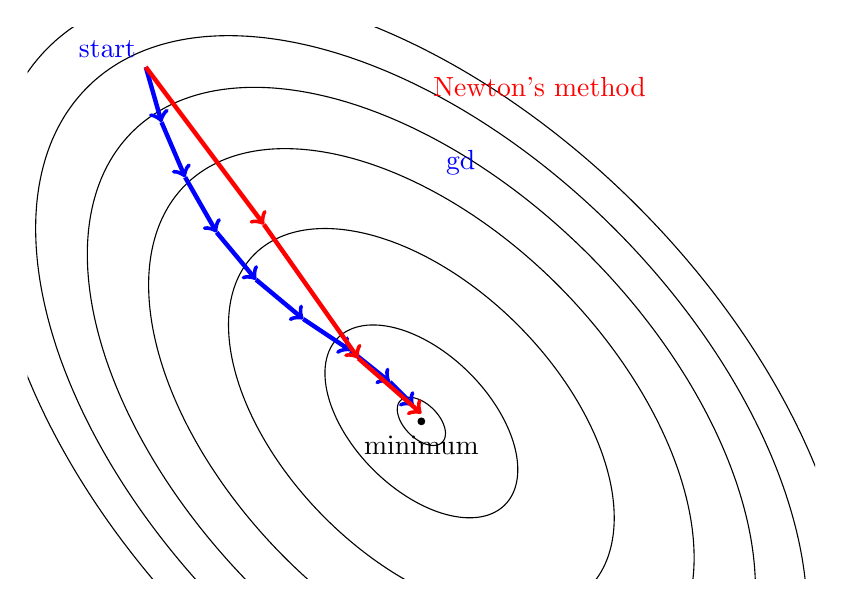
\begin{tikzpicture}[samples=200,smooth]
			\begin{scope}
				\clip(-5,-2) rectangle (5,5);
				\draw[thin] plot[domain=0:360] ({1.5*cos(\x)*sqrt(20/(sin(2*\x)+2))},{1.5*sin(\x)*sqrt(20/(sin(2*\x)+2))});
				\draw[thin] plot[domain=0:360] ({1.5*cos(\x)*sqrt(16/(sin(2*\x)+2))},{1.5*sin(\x)*sqrt(16/(sin(2*\x)+2))});
				\draw[thin] plot[domain=0:360] ({1.5*cos(\x)*sqrt(12/(sin(2*\x)+2))},{1.5*sin(\x)*sqrt(12/(sin(2*\x)+2))});
				\draw[thin] plot[domain=0:360] ({1.5*cos(\x)*sqrt(8/(sin(2*\x)+2))},{1.5*sin(\x)*sqrt(8/(sin(2*\x)+2))});
				\draw[thin] plot[domain=0:360] ({1.5*cos(\x)*sqrt(4/(sin(2*\x)+2))},{1.5*sin(\x)*sqrt(4/(sin(2*\x)+2))});
				\draw[thin] plot[domain=0:360] ({1.5*cos(\x)*sqrt(1/(sin(2*\x)+2))},{1.5*sin(\x)*sqrt(1/(sin(2*\x)+2))});
				\draw[thin] plot[domain=0:360] ({1.5*cos(\x)*sqrt(0.0625/(sin(2*\x)+2))},{1.5*sin(\x)*sqrt(0.0625/(sin(2*\x)+2))});
				% Gradient Descent path
				\draw[->,blue,ultra thick] (-3.5,4.5) -- (-3.3,3.8);
				\draw[->,blue,ultra thick] (-3.3,3.8) -- (-3,3.1);
				\draw[->,blue,ultra thick] (-3,3.1) -- (-2.6,2.4);
				\draw[->,blue,ultra thick] (-2.6,2.4) -- (-2.1,1.8);
				\draw[->,blue,ultra thick] (-2.1,1.8) -- (-1.5,1.3);
				\draw[->,blue,ultra thick] (-1.5,1.3) -- (-0.9,0.9);
				\draw[->,blue,ultra thick] (-0.9,0.9) -- (-0.4,0.5);
				\draw[->,blue,ultra thick] (-0.4,0.5) -- (-0.1,0.2);
				\node[blue,above left] at (-3.5,4.5) {start};
				\node[blue,above] at (0.5,3) {\gls{gd}};
				% Newton's Method path 
				\draw[->,red,ultra thick] (-3.5,4.5) -- (-2,2.5);
				\draw[->,red,ultra thick] (-2,2.5) -- (-0.8,0.8);
				\draw[->,red,ultra thick] (-0.8,0.8) -- (0,0.1);
				\node[red,above] at (1.5,4) {Newton's method};
				\node at (0,0) [circle,fill,inner sep=1pt,label=below:\gls{minimum}] {};
			\end{scope}
		\end{tikzpicture}
		\caption{Comparison of \gls{gd} (blue) and Newton's method (red) paths toward the \gls{minimum} of a 
			\gls{lossfunc}. \label{fig_newtonmethod_dict}}
		\end{figure}
		See also: \gls{optmethod}, \gls{gradient}, \gls{hessian}, \gls{gd}. },
  	first={newtonmethod},
 	type=math,
  	text={newtonmethod} 
}

\newglossaryentry{hilbertspace}
{name={Hilbert space},
 description={A \index{Hilbert space} Hilbert space $\hilbertspace$ is a complete 
    inner product space. Thus, $\hilbertspace$ is a \gls{vectorspace} 
	equipped with an inner product $\innerprod{\cdot}{\cdot}$. The inner product 
	induces a norm $\normgeneric{\cdot}{2}$ via $\normgeneric{\weights}{2} = \sqrt{\innerprod{\weights}{\weights}}$. 
  	Furthermore, $\hilbertspace$ is complete in the sense that every 
 	\gls{cauchysequence} $\big( \weights^{(\sampleidx)} \big)_{\sampleidx \in \mathbb{N}}$ 
	in $\hilbertspace$ converges to a limit $\lim_{\sampleidx\rightarrow \infty} \weights^{(\sampleidx)}$ 
	that is also contained in $\hilbertspace$. 
	\begin{figure}[H]
	\centering
	\begin{tikzpicture}[scale=3]
	% axes (light)
	%\draw[very thin, gray!30] (-1.2,0) -- (1.2,0);
	%\draw[very thin, gray!30] (0,-1.2) -- (0,1.2);
	% unit circle for visual context
	\draw[gray!40] (0,0) circle (1);
	% parameters
	\def\ang{35} % angle of v (degrees)
	% vectors
	\draw[->,thick] (0,0) -- (1,0) node[below right] {$\vu$};
	\draw[->,thick] (0,0) -- ({cos(\ang)},{sin(\ang)}) node[above] {$\vv$};
	% projection of v onto u
	\coordinate (P) at ({cos(\ang)},0);
	\draw[dashed] ({cos(\ang)},{sin(\ang)}) -- (P);
	\draw[->,thick] (0,0) -- (P) node[pos=0.5,below] {$\innerprod{\vv}{\vu} \vu$};
	% right-angle marker at foot of perpendicular
	\draw ($(P)+(0,0.06)$) -- (P) -- ($(P)+(-0.06,0)$);
	% angle arc and label
	%\draw (0.35,0) arc (0:\ang:0.35);
	%\node at ({0.48*cos(\ang/2)},{0.48*sin(\ang/2)}) {$\theta$};	
	% norm labels (unit vectors)
	%\node[below] at (1,0) {$\|\mathbf u\|=1$};
	\node[right] at ({cos(-\ang)},{sin(-\ang)}) {$\sphere{\nrfeatures} = \{ \weights \in \mathbb{R}^{\nrfeatures}: \innerprod{\weights}{\weights}=1\}$};
	% inner product hint
	%\node[below] at (P) {$\langle \mathbf u,\mathbf v\rangle=\cos\theta$};
\end{tikzpicture}
\caption{For two unit-norm vectors $\vu, \vv \in \sphere{\nrfeatures} \subseteq \mathbb{R}^{\nrfeatures}$ 
the inner product $\innerprod{\vu}{\vv}$ is the expantion coefficient for the projection 
of $\vv$ onto the subspace $\{ c \vu: c \in \reals \}$ spanned by $\vu$. 
The absolute value $|\innerprod{\vu}{\vv}|$ measures the norm of this projection.\label{fig_hilbertspace_dict}}
\end{figure}
	One important example of a Hilbert space 
 	is the \gls{euclidspace} $\mathbb{R}^{\nrfeatures}$ with the 
 	inner product $\innerprod{\weights}{\weights'} = \weights^{\top} \weights'$ \\
   	See also: \gls{vectorspace}.},
   	type=math, 
 	first = {Hilbert space}, 
    text = {Hilbert space},
   	plural={Hilbert spaces},
   	firstplural={Hilbert spaces}
  }

\newglossaryentry{cauchysequence}
{name={Cauchy sequence},
 description={A \index{Cauchy sequence} Cauchy \gls{sequence} is a \gls{sequence}
          $\big( \featurevec^{(\sampleidx)}\big)_{\sampleidx \in \mathbb{N}}$ 
		  in a \gls{metricspace} $\pair{\featurespace}{\metric{\cdot}{\cdot}}$ such 
		  that the elements $\featurevec^{(\sampleidx)}\in \featurespace$ 
		  become arbitrarily close to each other eventually. 
		  In other words \cite[Def. 3.8.]{RudinBookPrinciplesMatheAnalysis}, 
		  \[
		  \forall \epsilon > 0, \exists N \in \mathbb{N} \text{ such that } 
		  \forall \sampleidx, \sampleidx' \geq N, \ \metric{\featurevec^{(\sampleidx)}}{\featurevec^{(\sampleidx')}} < \epsilon.
		  \] 
		  \begin{figure}
			\centering
		  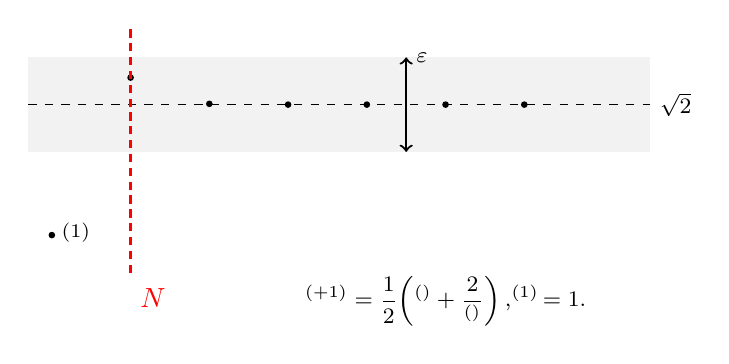
\begin{tikzpicture}[x=1cm,y=4cm]
			% Parameters
					\def\srtwo{1.4142}
					\def\eps{0.15}
					\def\nmax{7}
			% Axes
			%	\draw[->] (-0.3,0) -- (\nmax+0.6,0) node[right] {$\sampleidx$};
			%	\draw[->] (-0.3,0.9) -- (-0.3,1.46) node[above] {$x^{(\sampleidx)}$};
			% epsilon band around sqrt(2)
						\fill[gray!30, opacity=0.35]
						(-0.3,{\srtwo-\eps}) rectangle (\nmax+0.6,{\srtwo+\eps});
					%	\draw[dotted] (-0.3,{\srtwo+\eps}) -- (\nmax+0.6,{\srtwo+\eps})
					%	node[right] {\footnotesize{$\sqrt{2}+\varepsilon$}};
					%	\draw[dotted] (-0.3,{\srtwo-\eps}) -- (\nmax+0.6,{\srtwo-\eps})
				%		node[right] {\footnotesize{$\sqrt{2}-\varepsilon$}};
				% Double arrow showing epsilon band width
				\draw[<->, thick] (4.5,{\srtwo-\eps}) -- (4.5,{\srtwo+\eps})
				node[above, right] {\footnotesize{$\varepsilon$}};
						% Limit line at sqrt(2)
						\draw[dashed] (-0.3,\srtwo) -- (\nmax+0.6,\srtwo)
						node[right] {\footnotesize{$\sqrt{2}$}};
						% Sequence via fixed-point iteration: x_{n+1} = 0.5(x_n + 2/x_n), x_0 = 1
					      % Replace the foreach loop by:
					      \fill (0,1.0000) circle (1.2pt) node [right] {$\feature^{(1)}$};
					      \fill (1,1.5000) circle (1.2pt);
					      \fill (2,1.4167) circle (1.2pt);
					      \fill (3,1.4142) circle (1.2pt);
					      \fill (4,1.41421) circle (1.2pt);
					      \fill (5,1.4142136) circle (1.2pt);
					      \fill (6,1.41421356) circle (1.2pt);
			% Choose an N (first index within eps-band) -- here N=3 works for eps=0.005
						\def\N{1}
						\draw[densely dashed, thick, red] (\N,0.88) -- (\N,1.655);
						\node[right, red] at (\N,0.8) {$N$};
						% Formula box (fixed-point iteration)
						\node[align=right, anchor=north, font=\small]
						at (5,0.9)
						{\footnotesize{$\displaystyle \feature^{(\sampleidx+1)}=\frac{1}{2}\!\left(\feature^{(\sampleidx)}+\frac{2}{\feature^{(\sampleidx)}}\right), \feature^{(1)}=1.$}};
						% Optional: annotate a few rational iterates
			%			\node[font=\scriptsize, anchor=west] at (0,1.5-0.06) {$x^{(1)}=\tfrac{3}{2}$};
			%			\node[font=\scriptsize, anchor=west] at (1,1.5-0.12) {$x^{(2)}=\tfrac{17}{12}$};
			%			\node[font=\scriptsize, anchor=west] at (2,1.5-0.145) {$x^{(3)}=\tfrac{577}{408}$};
			\end{tikzpicture}
			\caption{A Cauchy \gls{sequence} 
			$\big(\feature^{(\sampleidx)}\big)_{\sampleidx\in\mathbb{N}}$ 
			in the \gls{metricspace} $\pair{\mathbb{Q}}{|\cdot|}$. 
			This \gls{sequence} is generated by a \gls{fixedpointiter} used to approximate 
			$\sqrt{2}$.  For all $\sampleidx \ge N$, 
			the \gls{sequence} elements lie within a band of width $\varepsilon$. 
			Note that the \gls{sequence} does not converge in $\mathbb{Q}$ 
			since $\sqrt{2} \notin \mathbb{Q}$ \cite[Example 1.1.]{RudinBookPrinciplesMatheAnalysis}.\label{fig:fpit_cauchy_sqrt2_dict}}
			\end{figure}
		   Fig.\ \ref{fig:fpit_cauchy_sqrt2_dict} shows a Cauchy sequence in the \gls{metricspace} $\pair{\mathbb{Q}}{|\cdot|}$ of 
		   rational numbers.  \\ 
		  See also: \gls{metricspace}, \gls{sequence}. }, 
		type=math,
		first={Cauchy sequence},
		text={Cauchy sequence},
		plural={Cauchy sequences},
		firstplural={Cauchy sequences}
}

\newglossaryentry{nonexpansiveop}
 {name={non-expansive operator},
 	description={An \index{non-expansive operator} operator 
	$\fixedpointop: \hilbertspace \rightarrow \hilbertspace$ defined on a 
	Hilbert space $\hilbertspace$ is called non-expansive if it does 
	not increase distances. 
	In other words,  
 		\begin{equation} 
 			\nonumber
 			\normgeneric{ \fixedpointop \weights - \fixedpointop \weights'}{2} 
			\leq 	\normgeneric{\weights - \weights'}{2} \mbox{ for any } \weights, \weights' \in \hilbertspace. 
 		\end{equation} 
 		See also: \gls{fixedpointiter}, \gls{contractop}.},
 	type=math, 
	first={non-expansive operator},
 	plural={non-expansive operators},
	firstplural={non-expansive operators},
 	text={non-expansive operator}
 }

\newglossaryentry{fixedpointiter}
{name={fixed-point iteration},
	description={A\index{fixed-point iteration} fixed-point iteration is an iterative method for solving 
		a given \gls{optproblem}. It constructs a sequence $\weights^{(0)}, \,\weights^{(1)}, \,\ldots$ by 
		 repeatedly applying an operator $\fixedpointop$, i.e., 
		 \begin{equation} 
		 	\label{equ_def_fixed_point_dict} 
		 	\weights^{(\iteridx+1)} = \fixedpointop \weights^{(\iteridx)} \mbox{, for } \iteridx=0, \,1, \,\ldots.
		 \end{equation} 
		 The operator $\fixedpointop$ is chosen such that any of its fixed points is a solution 
		 $\widehat{\weights}$ to the given \gls{optproblem}. For example, given a \gls{differentiable} and 
		 \gls{convex} \gls{function} $f(\weights)$, the fixed points of the operator $\fixedpointop: \weights \mapsto \weights - \nabla f(\weights)$ 
		 coincide with the minimizers of $f(\weights)$. In general, for a given \gls{optproblem} with solution $\widehat{\weights}$, 
		 there are many different operators $\fixedpointop$ whose fixed points are $\widehat{\weights}$. 
		 Clearly, we should use an operator $\fixedpointop$ in \eqref{equ_def_fixed_point_dict} that reduces the distance to a solution such that
		 \begin{equation} 
			\nonumber
			\underbrace{\normgeneric{ \weights^{(\iteridx+1)} - \widehat{\netparams}}{2}}_{\stackrel{\eqref{equ_def_fixed_point_dict}}{=} \normgeneric{ \fixedpointop \weights^{(\iteridx)} - \fixedpointop\widehat{\weights}}{2}}  \leq 	\normgeneric{ \weights^{(\iteridx)} - \widehat{\weights}}{2}. 
		\end{equation}
		Thus, we require $\fixedpointop$ to be at least non-expansive, i.e., the iteration \eqref{equ_def_fixed_point_dict} 
		should not result in worse \glspl{modelparam} that have a larger distance to a solution $\widehat{\weights}$. 
		Furthermore, each iteration \eqref{equ_def_fixed_point_dict} should also make some progress, i.e., 
		reduce the distance to a solution $\widehat{\weights}$. This requirement can be made precise using 
		the notion of a \gls{contractop} \cite{Bauschke:2017}, \cite{fixedpoinIsta}. 
		The operator $\fixedpointop$ is a \gls{contractop} if, for some $\contractfac \in [0,1)$,
		\begin{equation} 
			\nonumber
			\normgeneric{ \fixedpointop \weights\!-\!\fixedpointop \weights'}{2}  \leq  \contractfac	\normgeneric{\weights\!-\!\weights'}{2} \mbox{ holds for any } \weights,\weights'.
		\end{equation}
		For a \gls{contractop} $\fixedpointop$, the fixed-point iteration \eqref{equ_def_fixed_point_dict} generates 
		a sequence $\weights^{(\iteridx)}$ that converges quite rapidly. In particular \cite[Th. 9.23]{RudinBookPrinciplesMatheAnalysis}, 
		\begin{equation} 
			\nonumber
			\normgeneric{ \weights^{(\iteridx)} - \widehat{\weights}}{2} \leq \contractfac^{\iteridx} 	\normgeneric{ \weights^{(0)} - \widehat{\weights}}{2}. 
		\end{equation} 
		Here, $\normgeneric{ \weights^{(0)} - \widehat{\weights}}{2}$ is the distance between 
		the initialization $\weights^{(0)}$ and the solution $\widehat{\weights}$. 
		It turns out that a fixed-point iteration \eqref{equ_def_fixed_point_dict} with a firmly non-expansive 
		operator $\fixedpointop$ is guaranteed to converge to a fixed-point of $\fixedpointop$ \cite[Corollary 5.16]{Bauschke:2017}. 
		Fig. \ref{fig_examples_nonexp_dict} depicts examples of a firmly non-expansive operator, a non-expansive operator, 
		and a \gls{contractop}. All of these operators are defined on the 1-D space $\mathbb{R}$. 
		Another example of a firmly non-expansive operator is the \gls{proxop} of a \gls{convex} \gls{function} \cite{Bauschke:2017}, \cite{ProximalMethods}. 
		\definecolor{darkgreen}{rgb}{0.0, 0.5, 0.0}
		\begin{figure}[H]
			\begin{center} 
				\begin{tikzpicture}[scale=1.5]
					% Axes
					\draw[line width=1pt, ->] (-2,0) -- (2,0) node[right] {$\weight^{(\iteridx)}$};
					\draw[line width=1pt, ->] (0,-2) -- (0,2) node[above] {$\weight^{(\iteridx+1)}$};
					% Labels
					\node at (2.1,2.2) {$\fixedpointop^{(3)}$};
					\node at (1.9,-1.5) {$\fixedpointop^{(1)}$};
					\node at (1.5,1.2) {$\fixedpointop^{(2)}$};
					% Dashed lines at x=1 and y=1
					\draw[dashed] (1,-2) -- (1,2); % Vertical line at x=1
					\draw[dashed] (-2,1) -- (2,1); % Horizontal line at y=1
					\draw[dashed] (-2,-1) -- (2,-1); % Horizontal line at y=1
					\draw[dashed] (-1,-2) -- (-1,2); % Vertical line at x=1
					\node[above,xshift=4pt,yshift=-1pt] at (1,0) {$1$};
					\node[above,xshift=8pt,yshift=-1pt] at (0,-1) {$-1$};
					% First curve: y = 1/2 x + 1
					\draw[line width=2,domain=-2:2,smooth,blue] plot(\x,{0.5*\x + 1});
					% Second curve: y = -x
					\draw[line width=2,domain=-2:2,smooth,red] plot(\x,{-\x});
					% Third curve: y = x / |x| * min(|x|, 1)
					\draw[line width=2, domain=-2:-1,smooth,darkgreen] plot(\x,{-1});
					\draw[line width=2,domain=-1:1,smooth,darkgreen] plot(\x,{\x});
					\draw[line width=2,domain=1:2,smooth,darkgreen] plot(\x,{1});
				\end{tikzpicture}
			\end{center} 
			\caption{Example of a non-expansive operator $\fixedpointop^{(1)}$, a firmly non-expansive operator $\fixedpointop^{(2)}$, and 
				a \gls{contractop} $\fixedpointop^{(3)}$. \label{fig_examples_nonexp_dict}}
		\end{figure} 
		See also: \gls{optproblem}, \gls{differentiable}, \gls{convex}, \gls{function}, \glspl{modelparam}, \gls{contractop}, \gls{proxop}.},
	first={fixed-point iteration},
	text={fixed-point iteration},
	type=math, 
	firstplural={fixed-point iterations}, 
	plural={fixed-point iterations}
}


\newglossaryentry{ergraph}
{name={Erd\H{o}s–R\'enyi graph (ER graph)},
	description={An ER \gls{graph}\index{Erd\H{o}s–R\'enyi graph (ER graph)} is a \gls{probmodel} for \glspl{graph} defined over 
		a given node set $\nodeidx=1, \,\ldots, \,\nrnodes$. One way to define the ER \gls{graph} is 
		via the collection of \gls{iid} binary \glspl{rv} $b^{(\edge{\nodeidx}{\nodeidx'})} \in \{0,1\}$, 
		for each pair of different nodes $\nodeidx, \nodeidx'$. A specific \gls{realization}  
		of an ER \gls{graph} contains an edge $\edge{\nodeidx}{\nodeidx'}$ if and only if 
		$b^{(\edge{\nodeidx}{\nodeidx'})}=1$. The ER \gls{graph} is parameterized by the 
		number $\nrnodes$ of nodes and the \gls{probability} $\prob{b^{(\edge{\nodeidx}{\nodeidx'})}=1}$. 
		\\
		See also: \gls{graph}, \gls{probmodel}, \gls{iid}, \gls{rv}, \gls{realization}, \gls{probability}.},
	first={Erd\H{o}s–R\'enyi (ER) graph},
	text={ER graph}
}

\newglossaryentry{attack}
{name={attack},  
	description={An attack\index{attack} on an \gls{ml} system refers to an intentional action—either 
		active or passive—that compromises the system's integrity, availability, or confidentiality. 
		Active attacks involve perturbing components such as \glspl{dataset} (via \gls{datapoisoning}) 
		or communication links between \glspl{device} within an \gls{ml} application. Passive attacks, 
		such as \glspl{privattack}, aim to infer \glspl{sensattr} without modifying the system. 
		Depending on their goal, we distinguish among \glspl{dosattack}, \gls{backdoor} attacks, and \glspl{privattack}.
		\\
		See also: \gls{datapoisoning}, \gls{privattack}, \gls{sensattr}, \gls{dosattack}, \gls{backdoor}.},
	plural={attacks}, 
	first={attack},
	firstplural={attacks},
	text={attack}
}

\newglossaryentry{privattack}
{name={privacy attack},
	description={A privacy \gls{attack}\index{privacy attack} on an \gls{ml} system aims to infer 
		\glspl{sensattr} of individuals by exploiting partial access to a trained \gls{ml} \gls{model}. 
		One form of a privacy \gls{attack} is \gls{modelinversion}.\\
		See also: \gls{attack}, \gls{sensattr}, \gls{modelinversion}, \gls{trustAI}, \gls{gdpr}.},
	plural={privacy attacks}, 
	first={privacy attack},
	firstplural={privacy attacks}, 
	text={privacy attack}
}

\newglossaryentry{epigraph}
{name={epigraph},
  description={The epigraph\index{epigraph} of a real-valued \gls{function} $f : \mathbb{R}^n \to \mathbb{R} \cup \{+\infty\}$ 
  	is the set of points lying on or above its \gls{graph} (see Fig. \ref{fig_epigraph_dict}), i.e., 
		\[
		\operatorname{epi}(f) = \left\{ (\mathbf{x}, t) \in \mathbb{R}^n \times \mathbb{R} \,\middle|\, f(\mathbf{x}) \leq t \right\}.
		\]
		A \gls{function} is \gls{convex} if and only if its epigraph is a \gls{convex} set \cite{BoydConvexBook}, \cite{BertCvxAnalOpt}.
		\begin{figure}[H]
			\centering
			\begin{tikzpicture}[scale=1.0]
				\begin{axis}[
					axis lines = middle,
					xlabel = $x$,
					ylabel = {},
					xmin=-2, xmax=2,
					ymin=0, ymax=4.5,
					samples=100,
					domain=-1.5:1.5,
					thick,
					width=8cm,
					height=6cm,
					grid=none,
					axis on top,
					]
					% Function
					\addplot [blue, thick, domain=-1.5:1.5] {x^2} node [pos=0.85, anchor=south west, xshift=5pt] {$f(x)$};
					% Epigraph shading
					\addplot [
					name path=f,
					draw=none,
					ytick=\empty,
					domain=-1.5:1.5,
					] {x^2};
					\path[name path=top] (axis cs:-1.5,4) -- (axis cs:1.5,4);
					\addplot [
					blue!20,
					opacity=0.6,
					draw=none,
					] fill between [
					of=f and top,
					soft clip={domain=-1.5:1.5},
					];
					    \node[font=\small] at (axis cs:-1.0,2.3) {$\operatorname{epi}(f)$};
				%	\node[align=center, fill=white, draw=black, rounded corners, font=\small] at (axis cs:0.5,3.5) {Epigraph\\$\{(x,t) \mid f(x) \le t\}$};
				\end{axis}
			\end{tikzpicture}
			\caption{Epigraph of the \gls{function} $f(x) = x^2$ (i.e., the shaded area). \label{fig_epigraph_dict}}
		\end{figure}
		See also: \gls{function}, \gls{convex}.},
	first={epigraph},
	text={epigraph},
	plural={epigraphs}
}


\newglossaryentry{nullspace}
{name={nullspace},
	description={The nullspace\index{nullspace} of a \gls{matrix} $\mA \in \mathbb{R}^{\nrfeatures' \times \nrfeatures}$, 
		denoted by $\nullspace{\mA}$, is the set of all \glspl{vector} $\mathbf{n} \in \mathbb{R}^\nrfeatures$ 
    		such that $$\mA \mathbf{n} = \mathbf{0}.$$ 
		Consider a \gls{featlearn} method that uses the \gls{matrix} $\mA$ to transform 
		a \gls{featurevec} $\mathbf{x} \in \mathbb{R}^{\nrfeatures}$ of a \gls{datapoint} 
		into a new \gls{featurevec} $\vz = \mA \mathbf{x} \in \mathbb{R}^{\nrfeatures'}$. 
		The nullspace $\nullspace{\mA}$ characterizes all directions in the original 
    		\gls{featurespace} $\mathbb{R}^{\nrfeatures}$ along which the transformation 
		$\mA \mathbf{x}$ remains unchanged. In other words, adding any \gls{vector} from 
		the nullspace to a \gls{featurevec} $\featurevec$ does not affect the transformed 
		representation $\vz$. This property can be exploited to enforce invariances in the 
		\glspl{prediction} (computed from $\mA \mathbf{x}$). Fig.\ \ref{fig:nullspace-rotation-dict} 
		illustrates one such invariance. It shows rotated versions of two handwritten digits, 
		which approximately lie along 1-D curves in the original \gls{featurespace}. 
		These curves are aligned with a direction \gls{vector} $\mathbf{n} \in \mathbb{R}^{\nrfeatures}$. 
    		To ensure that the trained \gls{model} is invariant to such rotations, we can 
		choose the transformation \gls{matrix} $\mA$ such that $\mathbf{n} \in \nullspace{\mA}$. 
		This ensures that $\mA \mathbf{x}$, and hence the resulting \gls{prediction}, 
		is approximately insensitive to rotations of the input image.
		\begin{figure}[H]
      			\centering
      			\includegraphics[width=0.6\textwidth]{assets/pythonsnacks/nullspace_0_1.png}
	  		\caption{
			Rotated handwritings of two different digits. The rotations are approximately 
			aligned along straight lines parallel to the \gls{vector} $\mathbf{n}$. For a 
			binary \gls{classifier} distinguishing between these digits, a natural choice is 
			a linear \gls{featuremap} $\featurevec \mapsto \mathbf{A}\featurevec$ with a 
			\gls{matrix} $\mA$ whose nullspace contains $\mathbf{n}$, i.e., $\mathbf{n} \in \mathrm{null}(\mA)$.
                \label{fig:nullspace-rotation-dict}}	
	       	\end{figure}
		See also: \gls{matrix}, \gls{featuremap}, \gls{featlearn}. \\ 
		Python demo: \href{https://github.com/AaltoDictionaryofML/AaltoDictionaryofML.github.io/blob/main/assets/pythonsnacks/nullspace.py}{click me}},
 	first={nullspace},
 	firstplural={nullspaces},
 	plural={nullspaces},
 	text={nullspace}
}


\newglossaryentry{maximum}
{name={maximum},
	description={The maximum\index{maximum} of a set $\mathcal{A} \subseteq \mathbb{R}$ 
     		of real numbers is the greatest element in that set, if such an element exists. A set $\mathcal{A}$ 
     		has a maximum if it is bounded above and attains its \gls{supremum} \cite[Sec.~1.4]{RudinBookPrinciplesMatheAnalysis}.
				\\ 
		See also: \gls{supremum}.},
 	first={maximum},
 	firstplural={maxima},
 	plural={maxima},
 	text={maximum}
}

\newglossaryentry{supremum}
{name={supremum (or least upper bound)},
	description={The supremum\index{supremum (or least upper bound)} of a set of real numbers is 
		the smallest number that is greater than or equal to every element in the set. More formally, a 
		real number $a$ is the supremum of a set $\mathcal{A} \subseteq \mathbb{R}$ if: 1) $a$ 
		is an upper bound of $\mathcal{A}$; and 2) no number smaller than $a$ is an upper bound of $\mathcal{A}$. 
		Every non-empty set of real numbers that is bounded above has a supremum, even if it does 
		not contain its supremum as an element \cite[Sec.~1.4]{RudinBookPrinciplesMatheAnalysis}.},
	firstplural={suprema}, 
  	plural={suprema},
	first={supremum (or least upper bound)},
	text={supremum}
}

\newglossaryentry{discrepancy}
{name={discrepancy},
	description={Consider\index{discrepancy} an \gls{fl} application with \gls{netdata} 
		represented by an \gls{empgraph}. \gls{fl} methods use a discrepancy measure 
		to compare \gls{hypothesis} \glspl{map} from \glspl{localmodel} at nodes $\nodeidx,\nodeidx'$, 
		connected by an edge in the \gls{empgraph}.
					\\ 
		See also: \gls{fl}, \gls{empgraph}, \gls{localmodel}.},
	first={discrepancy},
	firstplural={discrepancies}, 
  	plural={discrepancies}, 
	text={discrepancy}
}

\newglossaryentry{FedRelax}
{name={federated relaxed (FedRelax)},
	description={An\index{federated relaxed (FedRelax)} \gls{fl} \gls{distributedalgorithm}. 
		\\ 
		See also: \gls{fl}, \gls{distributedalgorithm}.},
	first={FedRelax},
	text={FedRelax}
} 

\newglossaryentry{fedavg}
{name={federated averaging (FedAvg)},
	description={FedAvg\index{federated averaging (FedAvg)} refers to a family of iterative \gls{fl} \glspl{algorithm}. 
		It uses a server-client setting and alternates between clientwise \glspl{localmodel} 
		retraining, followed by the aggregation of updated \glspl{modelparam} at the server 
		\cite{pmlr-v54-mcmahan17a}. The local update at client $\nodeidx=1, \,\ldots, \,\nrnodes$ 
		at time $\iteridx$ starts from the current \glspl{modelparam} $\weights^{(\iteridx)}$ provided 
		by the server and typically amounts to executing few iterations of \gls{stochGD}. After completing the local updates, they are aggregated 
		by the server (e.g., by averaging them). Fig. \ref{fig_single_iteration_fedavg_dict} illustrates the execution of a single 
		iteration of FedAvg. 
		\begin{figure}[H]
			\begin{center}
			\begin{tikzpicture}[>=Stealth, node distance=1cm and 1.5cm, every node/.style={font=\small}]
			% Styles
			\tikzstyle{server} = [circle, fill=black, minimum size=6pt, inner sep=0pt]
			\tikzstyle{client} = [circle, draw=black, minimum size=6pt, inner sep=0pt]
			% Time step labels
			\node (label1) at (0,3.5) {broadcast};
			\node[right=2.5cm of label1] (label2) {local update};
			\node[right=2.5cm of label2] (label3) {aggregate};
			% Time step k
			\node[server] (s1) at (label1 |- 0,2.5) {};
			\node[client] (c1l) at ($(s1) + (-1cm,-1cm)$) {};
			\node[client] (c1r) at ($(s1) + (1cm,-1cm)$) {};
			\node[] (dots1) at ($(s1) + (0cm,-1cm)$) {\ldots};
			\draw[->] (s1) -- (c1l) node[midway,left] {$\weights^{(\iteridx)}$};
			\draw[->] (s1) -- (c1r) node[midway,right] {$\weights^{(\iteridx)}$};
			\draw[->] (s1) -- (dots1);
			% Time step k+1 (local updates)
			\node[server] (s2) at (label2 |- 0,2.5) {};
			\node[client] (c2l) at ($(s2) + (-1cm,-1cm)$) {};
			\node[client] (c2r) at ($(s2) + (1cm,-1cm)$) {};
			\node[] (dots2) at ($(s2) + (0cm,-1cm)$) {\ldots};
			\node[below=0.2cm of c2l] {$\localparamsiter{\iteridx}{1}$};
			\node[below=0.2cm of c2r] {$\localparamsiter{\iteridx}{\nrnodes}$};
			% Time step k+2 (aggregation)
			\node[server] (s3) at (label3 |- 0,2.5) {};
			\node[above=0.01cm of s3, yshift=-4pt] {$\weights^{(\iteridx+1)}$};
			\node[client] (c3l) at ($(s3) + (-1cm,-1cm)$) {};
			\node[client] (c3r) at ($(s3) + (1cm,-1cm)$) {};
			\node[] (dots3) at ($(s3) + (0cm,-1cm)$) {\ldots};
			\draw[->] (c3l) -- (s3) node[midway,left] {$\localparamsiter{\iteridx}{1}$};
			\draw[->] (c3r) -- (s3)  node[midway,right] {$\localparamsiter{\iteridx}{\nrnodes}$};
			\draw[->] (dots3) -- (s3);
			\end{tikzpicture}
			\end{center}
			\caption{Illustration of a single iteration of FedAvg, which consists of broadcasting \glspl{modelparam} by the 
			server, performing local updates at clients, and aggregating the updates by the server. 
			\label{fig_single_iteration_fedavg_dict}} 
		\end{figure} 
		See also: \gls{fl}, \gls{algorithm}, \gls{localmodel}, \gls{stochGD}.},
	first={FedAvg},
	text={FedAvg}
} 

\newglossaryentry{FedGD}
{name={federated gradient descent (FedGD)},
	description={An\index{federated gradient descent (FedGD)} \gls{fl} \gls{distributedalgorithm} that 
		can be implemented as message passing across an \gls{empgraph}. 
		\\ 
		See also: \gls{fl}, \gls{distributedalgorithm}, \gls{empgraph}, \gls{gradstep}, \gls{gdmethod}.},
	first={FedGD},
	text={FedGD}
} 

\newglossaryentry{FedSGD}
{name={federated stochastic gradient descent (FedSGD)},
	description={An\index{federated stochastic gradient descent (FedSGD)} \gls{fl} \gls{distributedalgorithm} that 
		can be implemented as message passing across an \gls{empgraph}. 
		\\ 
		See also: \gls{fl}, \gls{distributedalgorithm}, \gls{empgraph}, \gls{gradstep}, \gls{gdmethod}, \gls{stochGD}.},
	first={FedSGD},
	text={FedSGD}
} 

\newglossaryentry{hfl}
{name={horizontal federated learning (HFL)},
	description={HFL\index{horizontal federated learning (HFL)} uses \glspl{localdataset} constitut\-ed by different
	   	\glspl{datapoint} but uses the same \glspl{feature} to characterize them \cite{HFLChapter2020}.
		For example, weather forecasting uses a network of spatially distributed
		weather (observation) stations. Each weather station measures the
		same quantities, such as daily temperature, air pressure, and precipitation.
		However, different weather stations measure the characteristics or
		\glspl{feature} of different spatiotemporal regions. Each spatiotemporal region 
		represents an individual \gls{datapoint}, each characterized by the same \glspl{feature} 
		(e.g., daily temperature or air pressure).\\
		See also: \gls{ssl}, \gls{fl}, \gls{vfl}.},
	first={horizontal federated learning (HFL)},
	text={HFL}
} 

\newglossaryentry{dimred}
{name={dimensionality reduction},
	description={Dimensionality reduction\index{dimensionality reduction} refers 
		to methods that learn a transformation 
		$\hypothesis: \mathbb{R}^{\nrfeatures} \rightarrow \mathbb{R}^{\nrfeatures'}$ 
		of a (typically large) set of raw \glspl{feature} $\feature_{1}, \,\ldots, \,\feature_{\nrfeatures}$ 
		into a smaller set of informative \glspl{feature} $z_{1}, \,\ldots, \,z_{\nrfeatures'}$. 
		Using a smaller set of \glspl{feature} is beneficial in several ways: 
		\begin{itemize} 
			\item {Statistical benefit:} It typically reduces the \gls{risk} of \gls{overfitting}, as 
			reducing the number of \glspl{feature} often reduces the \gls{effdim} of a \gls{model}. 
			\item {Computational benefit:} Using fewer \glspl{feature} means less computation 
			for the training of \gls{ml} \glspl{model}. As a case in point, \gls{linreg} methods 
			need to invert a \gls{matrix} whose size is determined by the number of \glspl{feature}. 
			\item {Visualization:} Dimensionality reduction is also instrumental for \gls{data} visualization. 
			For example, we can learn a transformation that delivers two \glspl{feature} $z_{1},z_{2}$, 
			which we can use, in turn, as the coordinates of a \gls{scatterplot}. Fig.\ \ref{fig:dimred-scatter_dict} 
			depicts the \gls{scatterplot} of handwritten digits that are placed 
			using transformed \glspl{feature}. Here, the \glspl{datapoint} are 
			naturally represented by a large number of greyscale values (one value for each pixel).
		\end{itemize} 
		 \begin{figure}[H]
		 \centering
		 \begin{tikzpicture}[scale=1]	
		% % Axes
		 	\draw[->] (-0.5,0) -- (5.5,0) node[right] {$z_1$};
		 	\draw[->] (0,-0.5) -- (0,4.5) node[above] {$z_2$};
		% % Example points with mini-images (can replace adjustbox with \includegraphics)
		 	\foreach \x/\y/\label in {
  		 		1.2/0.5/3,
  		 		0.8/2.0/8,
  		 		2.5/1.8/1,
  		 		3.8/3.5/6,
  		 		4.2/0.7/9,
  		 		2.8/3.0/7,
  		 		1.5/3.8/2
		 	}{
  		 		\node[draw, minimum size=0.6cm, inner sep=0pt] at (\x,\y)
    	 		{\label};
		 	}
		 	\end{tikzpicture}
		 	\caption{Example of dimensionality reduction: High-dimensional image data 
			(e.g., high-resolution images of handwritten digits) embedded into 2-D using 
			learned \glspl{feature} $(z_1, z_2)$ and visualized in a \gls{scatterplot}.}
		 	\label{fig:dimred-scatter_dict}
		 \end{figure}
		See also: \gls{overfitting}, \gls{effdim}, \gls{model}, \gls{scatterplot}, \gls{pca}, \gls{johnsonlindenstrausslemma}.}, 
	first={dimensionality reduction},
	text={dimensionality reduction}
} 


\newglossaryentry{diagnosis}
{name={diagnosis},
	description={Consider\index{diagnosis} an \gls{erm}-based method that resulted in a trained \gls{model} 
	(or learned \gls{hypothesis}) $\learnthypothesis \in \hypospace$. We can diagnose the 
	method by comparing the \gls{trainerr} $\trainerror$ with the \gls{valerr} $\valerror$ 
	incurred by $\learnthypothesis$ on the \gls{trainset} and the \gls{valset}. 
	\begin{figure}[htbp]
	\begin{center}
		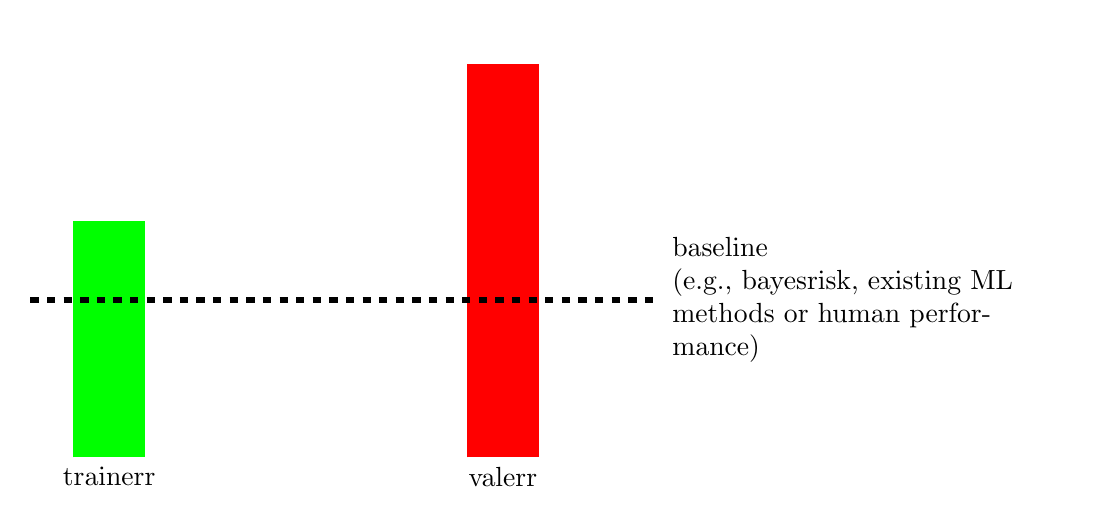
\begin{tikzpicture}[ycomb]
			\draw[color=green,line width=26pt]
			plot coordinates{(0,3)};
			\node [below] at (0,0) {\gls{trainerr}} ; 
			\draw[color=red,line width=26pt]
			plot coordinates{(5,5)};
			\node [below] at (5,0) {\gls{valerr}} ; 
			\draw[dashed,line width=2] (-1,2) -- (7,2) node[right,text width=5cm]{\gls{baseline} \\ (e.g., \gls{bayesrisk}, existing ML methods or human performance)};
		\end{tikzpicture}
	\end{center}
	\caption{We can diagnose a \gls{erm}-based \gls{ml} method by comparing its \gls{trainerr} 
		with its \gls{valerr}. Ideally both are on the same level as a \gls{baseline}.\label{fig_diagnosis_dict}}
		\end{figure}
	 			\\ 
		See also: \gls{validation}, \gls{kfoldcv}, \gls{generalization}, \gls{baseline}.},
	first={diagnosis},
	text={diagnosis}
} 


\newglossaryentry{ml}
{name={machine learning (ML)},
	description={ML\index{machine learning (ML)} aims to predict 
	 	a \gls{label} from the \glspl{feature} of a \gls{datapoint}. ML methods achieve 
	 	this by learning a \gls{hypothesis} from a \gls{hypospace} (or \gls{model}) 
	 	through the minimization of a \gls{lossfunc} \cite{MLBasics}, \cite{HastieWainwrightBook}. 
	 	One precise formulation of this principle is \gls{erm}. Different ML methods are 
	 	obtained from different design choices for \glspl{datapoint} (i.e., their \glspl{feature} and \gls{label}), 
	 	the \gls{model}, and the \gls{lossfunc} \cite[Ch. 3]{MLBasics}.
	 			\\ 
		See also: \gls{model}, \gls{data}, \gls{loss}.},
	first={machine learning (ML)},
	text={ML}
} 


\newglossaryentry{reinforcementlearning}
{name={reinforcement learning (RL)},
	description={RL\index{reinforcement learning (RL)} refers to an \gls{onlinelearning} setting where 
		we can only evaluate the usefulness of a single \gls{hypothesis} (i.e., a choice of \glspl{modelparam}) 
		at each time step $\timeidx$. In particular, RL methods apply the current \gls{hypothesis} 
		$\hypothesis^{(\timeidx)}$ to the \gls{featurevec} $\featurevec^{(\timeidx)}$ of the 
		newly received \gls{datapoint}. The usefulness of the resulting \gls{prediction} 
		$\hypothesis^{(\timeidx)}(\featurevec^{(\timeidx)})$ is quantified by a \gls{reward} 
		signal $\reward^{(\timeidx)}$ (see Fig. \ref{fig_reinforcementlearning_dict}). 
		\begin{figure}[H]
		\begin{center}
			\begin{tikzpicture}[scale=1]
			\draw[->] (-2, 0) -- (6, 0);
			\node at (6.3, 0) {$\hypothesis$};
	        		% loss at time t 
			\draw[thick, blue, domain=0:3, samples=20] plot (\x-3, {-0.2*(\x)^2 + 2});
			\node[anchor=west,yshift=4pt] at (0-3, {-0.2*(0)^2 + 2}) {$-\loss^{(\timeidx)}(\hypothesis)$};
			% Marker and hypothesis label for h^(t)
			\filldraw[blue] (1.5-3, {-0.2*(1.5)^2 + 2}) circle (2pt);
			\node[anchor=north] at (1.5-3, -0.3) {$\hypothesis^{(\timeidx)}$};		
			\draw[dotted] (1.5-3, 0) -- (1.5-3, {-0.2*(1.5)^2 + 2});
			%%% time t+1
			\draw[thick, red, domain=0:5, samples=20, dashed] plot (\x, {-0.15*(\x - 2)^2 + 3});
			\node[anchor=west,yshift=4pt] at (3, {-0.15*(3 - 2)^2 + 3}) {$-\loss^{(\timeidx+1)}(\hypothesis)$};
			\filldraw[red] (2, {-0.15*(2 - 2)^2 + 3}) circle (2pt);
			\node[anchor=north] at (2, -0.3) {$\hypothesis^{(\timeidx+1)}$};
			\draw[dotted] (2, 0) -- (2, {-0.15*(3 - 2)^2 + 3});
			%%% time t+2
			\draw[thick, green!60!black, domain=3:5, samples=20, dotted] plot (\x+2, {-0.1*(\x - 4)^2 + 1.5});
			\node[anchor=west,yshift=4pt] at (4.5+2, {-0.1*(4.5 - 4)^2 + 1.5}) {$-\loss^{(\timeidx+2)}(\hypothesis)$};
			\filldraw[green!60!black] (3.5+2, {-0.1*(3.5 - 4)^2 + 1.5}) circle (2pt);
			\node[anchor=north] at (3.5+2, -0.3) {$\hypothesis^{(\timeidx+2)}$};
			\draw[dotted] (3.5+2, 0) -- (3.5+2, {-0.1*(3.5 - 4)^2 + 1.5});
			\end{tikzpicture}
		\caption{Three consecutive time steps $\timeidx,\timeidx+1,\timeidx+2$ with corresponding \glspl{lossfunc} $\loss^{(\timeidx)},
		\loss^{(\timeidx+1)}, \loss^{(\timeidx+2)}$. During time step $\timeidx$, an RL method can evaluate the 
		\gls{lossfunc} only for one specific \gls{hypothesis} $\hypothesis^{(\timeidx)}$, resulting in the \gls{reward} 
		signal $\reward^{(\timeidx)}=-\loss^{(\timeidx)}(\hypothesis^{(\timeidx)})$. \label{fig_reinforcementlearning_dict}}
		\end{center}
		\end{figure}
		In general, the \gls{reward} depends also on the 
		previous \glspl{prediction} $\hypothesis^{(\timeidx')}\big(\featurevec^{(\timeidx')}\big)$ 
		for $\timeidx' < \timeidx$. The goal of RL is to learn $\hypothesis^{(\timeidx)}$, for 
		each time step $\timeidx$, such that the (possibly discounted) cumulative \gls{reward} 
		is maximized \cite{MLBasics}, \cite{SuttonEd2}.
		\\
		See also: \gls{reward}, \gls{lossfunc}, \gls{ml}.},
	first={reinforcement learning (RL)},
	text={RL}
}


\newglossaryentry{featlearn}
{name={feature learning},
	description={Consider an \gls{ml} application with \glspl{datapoint} characterized by 
		raw \glspl{feature} $\featurevec \in \featurespace$. \Gls{feature} learning\index{feature learning} 
		refers to the task of learning a \gls{map} 
		$$\featuremapvec: \featurespace \rightarrow \featurespace': \featurevec \mapsto \featurevec'$$ 
		that reads in the \glspl{feature} $\featurevec \in \featurespace$ of a \gls{datapoint} and delivers new 
		\glspl{feature} $\featurevec' \in \featurespace'$ from a new \gls{featurespace} $\featurespace'$. 
		Different \gls{feature} learning methods are obtained for different design 
		choices of $\featurespace,\featurespace'$, for a \gls{hypospace} $\hypospace$ 
		of potential \glspl{map} $\featuremapvec$, and for a quantitative measure of the usefulness of 
		a specific $\featuremapvec \in \hypospace$. For example, \gls{pca} 
		uses $\featurespace \defeq \mathbb{R}^{\dimlocalmodel}$, $\featurespace' \defeq \mathbb{R}^{\dimlocalmodel'}$ 
		with $\dimlocalmodel' < \dimlocalmodel$, and a \gls{hypospace} 
		$$\hypospace\defeq \big\{ \featuremapvec: \mathbb{R}^{\dimlocalmodel}
		\!\rightarrow\! \mathbb{R}^{\dimlocalmodel'}\!:\!\featurevec'\!\defeq\!\mF \featurevec \mbox{ with some } \mF \!\in\! \mathbb{R}^{\dimlocalmodel' \!\times \dimlocalmodel} \big\}.$$ \Gls{pca} measures the usefulness of a specific \gls{map} $\featuremapvec(\featurevec)= \mF \featurevec$ 
	by the \gls{minimum} linear reconstruction error incurred on a \gls{dataset} such that 
$$\min_{\mG \in \mathbb{R}^{\dimlocalmodel \!\!\!\times \dimlocalmodel'}} \sum_{\sampleidx=1}^{\samplesize} \normgeneric{\mG \mF \featurevec^{(\sampleidx)} - \featurevec^{(\sampleidx)}}{2}^{2}.$$ 
			\\ 
		See also: \gls{feature}, \gls{featurespace}, \gls{hypospace}, \gls{pca}.}, 
	first={feature learning},
	text={feature learning}
} 

\newglossaryentry{autoencoder}
{name={autoencoder},
	description={An autoencoder\index{autoencoder} is an \gls{ml} method that simultaneously 
		learns an encoder \gls{map} $\hypothesis \in \hypospace$ and a decoder \gls{map} 
		$\hypothesis^{*} \in \hypospace^{*}$. Different autoencoders use different 
		\glspl{model} $\hypospace, \hypospace^{*}$, e.g., \glspl{ann} with different architectures. 
        The special case of an autoeencoder using (vector-valued) \glspl{linmodel} for 
		$\hypospace, \hypospace^{*}$ results in \gls{pca}. 
		\begin{figure}[H]
		\centering
		\begin{tikzpicture}[>=Latex, thick, node distance=1.6cm]
		% Nodes
		\node (x) {$\vx$};
		\node[draw, rounded corners, right=of x, inner sep=4pt] (enc) {$\text{encoder } \hypothesis$};
		\node[right=of enc] (z) {$\vz$};
		\node[draw, rounded corners, right=of z, inner sep=4pt] (dec) {$\text{decoder } \hypothesis^{*}$};
		\node[right=of dec] (xhat) {$\hat{\featurevec}$};
		% Arrows
		\draw[->] (x) -- (enc);
		\draw[->] (enc) -- node[above] {$\vz=\hypothesis(\featurevec)$} (z);
		\draw[->] (z) -- (dec);
		\draw[->] (dec) -- node[above] {$\hat{\featurevec}=\hypothesis^{*}(\vz)$} (xhat);
		% (Optional) reconstruction loss
		%\draw[->, dashed] ($(xhat.south)+(0,-0.2)$) to[bend right=20] node[below] {$\loss$} ($(x.south)+(0,-0.2)$);
		\end{tikzpicture}
		\caption{Autoencoder with encoder $\hypothesis$ mapping $\featurevec \mapsto \vz$ and 
		decoder $\hypothesis^*$ mapping $\vz \mapsto \hat{\featurevec}$.}
		\end{figure}
		The training of the encoder and decoder can be implemented via \gls{erm} using a \gls{loss} that measures 
		the deviation of the reconstructed \gls{featurevec} $\hypothesis^{*}\big(\hypothesis\big(\featurevec \big) \big)$
		from the original \gls{featurevec} $\featurevec$.
					\\ 
		See also: \gls{featlearn}, \gls{dimred}.},
	first={autoencoder},
	text={autoencoder}
} 

\newglossaryentry{vfl}
{name={vertical federated learning (VFL)},
	description={VFL\index{vertical federated learning (VFL)} refers to \gls{fl} applications where  
		\glspl{device} have access to different \glspl{feature} of the same set of \glspl{datapoint} \cite{VFLChapter}. 
		Formally, the underlying global \gls{dataset} is
		\[
		\dataset^{(\mathrm{global})} \defeq \left\{ \left(\featurevec^{(1)}, \truelabel^{(1)}\right), \,\ldots, \,\left(\featurevec^{(\samplesize)}, \truelabel^{(\samplesize)}\right) \right\}.
		\]
		We denote by $\featurevec^{(\sampleidx)} = \big( \feature^{(\sampleidx)}_{1}, \,\ldots, \,\feature^{(\sampleidx)}_{\nrfeatures'} \big)\,^{T}$, for $\sampleidx=1, \,\ldots, \,\samplesize$, 
	     	the complete \glspl{featurevec} for the \glspl{datapoint}. Each \gls{device} $\nodeidx \in \nodes$ 
		observes only a subset $\mathcal{F}^{(\nodeidx)} \subseteq \{1, \,\ldots, \,\nrfeatures'\}$ of \glspl{feature}, resulting 
		in a \gls{localdataset} $\localdataset{\nodeidx}$ with \glspl{featurevec}
		\[
		\featurevec^{(\nodeidx,\sampleidx)} = \big( \feature^{(\sampleidx)}_{\featureidx_{1}}, \,\ldots, \,\feature^{(\sampleidx)}_{\featureidx_{\nrfeatures}} \big)\,^{T}.
		\]
		Some of the \glspl{device} may also have access to the \glspl{label} $\truelabel^{(\sampleidx)}$, for $\sampleidx=1, \,\ldots, \,\samplesize$, 
		of the global \gls{dataset} (see Fig. \ref{fig_vertical_FL_dict}). 
		\begin{figure}[H]
			\begin{center}
			\begin{tikzpicture}[every node/.style={anchor=base}]
				  % --- Coordinate definitions ---
				\def\colX{0}
				\def\colY{1.6}
				\def\colZ{3.2}
				\def\colD{4.8}
				\def\colLabel{6.4} 
				\def\rowOne{0}
				\def\rowTwo{-1.2}
				\def\rowThree{-2.4}
				\def\rowFour{-3.6}
				% Manually place matrix entries
				\foreach \i/\label in {1/1, 2/2, 4/\samplesize} {
					\pgfmathsetmacro{\y}{-1.2*(\i-1)}
					\node (x\i1) at (0,\y) {$x^{(\label)}_{1}$};
					\node (x\i2) at (1.6,\y) {$x^{(\label)}_{2}$};
					\node (dots\i) at (3.2,\y) {$\cdots$};
					\node (x\i3) at (4.8,\y) {$x^{(\label)}_{\dimlocalmodel}$};
					\node (y\i) at (6.4,\y) {$\truelabel^{(\label)}$};
				}
				  % Outer rectangle for the full dataset
				\draw[dashed, rounded corners, thick]
				(-0.6,0.6) rectangle (6.9,-4.2);
				\node at (3.1,0.9) {$\dataset^{(\mathrm{global})} $};
			% Rectangle for local dataset 1 (e.g., first two features)
			\draw[dashed, rounded corners, thick]
			(-0.9,0.9) rectangle (2.1,-4.0);
			\node at (0.25,1.0) {$\localdataset{1}$};
		  	% --- Local dataset k (columns 2–3, rows 1–3) ---
			\draw[dashed, rounded corners, thick]
			($( \colZ + 1,,0.9 )$) rectangle
			($( \colLabel + 0.4, -4.5)$);
				\node at ($( \colZ + 0.9,-5 )$) {$\localdataset{\nodeidx}$};
			\end{tikzpicture}
			\end{center}
			\caption{VFL uses \glspl{localdataset} that are derived from the \glspl{datapoint} of a common global \gls{dataset}. 
				The \glspl{localdataset} differ in the choice of \glspl{feature} used to characterize the \glspl{datapoint}.\label{fig_vertical_FL_dict}}
		\end{figure}
		One potential application of VFL is to enable collaboration between 
		different healthcare providers. Each provider collects distinct types of measurements—such as blood 
		values, electrocardiography, and lung X-rays—for the same patients. Another application is a 
		national social insurance system, where health records, financial indicators, consumer behavior, 
		and mobility \gls{data} are collected by different institutions. VFL enables joint learning across 
		these parties while allowing well-defined levels of \gls{privprot}.
		\\
		See also: \gls{fl}, \gls{privprot}.},
	first={vertical federated learning (VFL)},
	text={VFL}
} 

\newglossaryentry{interpretability}
{name={interpretability},
	description={An \gls{ml} method is interpretable\index{interpretability} for a 
 		human user if they can comprehend the decision process of the method. 
		One approach to develop a precise definition of interpretability is via the concept  
 		of simulatability, i.e., the ability of a human to mentally simulate the \gls{model} behavior 
		\cite{Colin:2022aa}, \cite{Chen2018}, \cite{doshi2017towards}, \cite{hase-bansal-2020-evaluating}, \cite{Lipton2018}. 
 		The idea is as follows: If a human user understands an \gls{ml} method, then they should 
 		be able to anticipate its \glspl{prediction} on a \gls{testset}. We illustrate 
 		such a \gls{testset} in Fig. \ref{fig_aug_simulatability_dict}, which also depicts 
		two learned \glspl{hypothesis} $\learnthypothesis$ and $\learnthypothesis'$. 
		The \gls{ml} method producing the \gls{hypothesis} $\learnthypothesis$ is interpretable
		to a human user familiar with the concept of a \gls{linearmap}. 
    		Since $\learnthypothesis$ corresponds to a \gls{linearmap}, the user can 
		anticipate the \glspl{prediction} of $\learnthypothesis$ on the 
		\gls{testset}. In contrast, the \gls{ml} method delivering $\learnthypothesis'$ 
		is not interpretable, because its behavior is no longer aligned with the user’s 
		\glspl{expectation}.
 		\begin{figure}[H]
 			\begin{center} 
			\begin{tikzpicture}[x=1.5cm, y=1cm]
  			% Adjustable parameters
 			\def\slope{0.4}
  			\def\offset{2.0}
  			% Axes
  			\draw[->, very thick] (0,0.5) -- (7.7,0.5) node[below, xshift=-1cm] {$\feature$}; % x-axis
 			\draw[->, very thick] (0.5,0) -- (0.5,4.2) node[above] {$\truelabel$};           % y-axis
  			% Model line
  			\draw[color=black, thick, dashed, domain=-0.5:7.2, variable=\x] 
    			plot ({\x},{\slope*\x + \offset});
			% non-interpretable model
  			\draw[color=black, thick, dashed, domain=4:7.2, variable=\x] 
    			plot ({\x},{\slope*\x + \offset-(\x-4)*0.5});
  			\node[above] at (7.2, {\slope*7.2 + \offset}) {$\learnthypothesis(\feature)$};
  			\node[above] at (7.2, {\slope*7.2 + \offset - 0.5*(7.2 - 4)}) {$\learnthypothesis'(\feature)$};
 			%\node[above] at (7.2, {\slope*7.2 + \offset-(7.2-4)*0.3}) {$\learnthypothesis'(\feature)$};
  			% Training Data points
  			\foreach \x/\y/\c/\s in {
      			1.2/1.0/blue/6, 1.4/1.0/blue/6, 1.7/1.0/blue/6,
      			2.2/3.9/blue/12, 2.6/4.2/blue/12, 3.0/4.4/blue/12
  			}{
    			\coordinate (pt) at (\x,\y);
    			\node[fill=\c, circle, draw, minimum size=\s pt, scale=0.6] at (pt) {};
    			\draw[<->, >={Latex[width=2mm,length=4mm]}, color=\c, thick]
      			(\x, {\slope*\x + \offset}) -- (pt);
  			}
  			% test set with pseudo-labels
    			\foreach \x/\y/\c/\s in {
       			5.7/2.6/red/12, 5.9/2.6/red/12, 6.2/2.6/red/12
   			}{
     			\coordinate (pt) at (\x,{\slope*\x + \offset});
     			\node[fill=\c, circle, draw, minimum size=\s pt, scale=0.6] at (pt) {};
   			}
  			% Legend
  			\draw[fill=blue] (4.2, 1.7) circle (0.1cm) node [black,xshift=0.2cm,anchor=west] {\gls{trainset} $\dataset$};
  			\draw[fill=red]  (4.2, 1.2) circle (0.1cm) node [black,xshift=0.2cm,anchor=west] {\gls{testset} $\dataset'$};
			\end{tikzpicture}
 			\caption{We can assess the interpretability of trained \gls{ml} \glspl{model} 
 			$\learnthypothesis$ and $\learnthypothesis'$ by comparing their \glspl{prediction} 
			to pseudo-\glspl{label} generated by a human user for $\dataset'$. 
			\label{fig_aug_simulatability_dict}}
 			\end{center}
	 	\end{figure} 
 	 	The notion of interpretability is closely related to the notion of \gls{explainability}, 
 	 	as both aim to make \gls{ml} methods more understandable for humans. 
		In the context of Fig. \ref{fig_aug_simulatability_dict}, interpretability of an \gls{ml} 
	 	method $\learnthypothesis$ requires that the human user can anticipate its \glspl{prediction} 
	 	on an arbitrary \gls{testset}. This contrasts with \gls{explainability}, where the user is supported by 
	 	external \glspl{explanation}—such as saliency \glspl{map} or reference examples from the \gls{trainset}—to 
		understand the \glspl{prediction} of $\learnthypothesis$ on a specific \gls{testset} $\dataset'$. 
	 	\\ 
	 	See also: \gls{explainability}, \gls{trustAI}, \gls{regularization}, \gls{lime}. },
	first={interpretability},
 	text={interpretability}
}

\newglossaryentry{multitask learning}
{name={multitask learning},
	description={Multitask learning\index{multitask learning} aims to leverage relations between 
	 	different \glspl{learningtask}. Consider two \glspl{learningtask} obtained from the 
	 	same \gls{dataset} of webcam snapshots. The first task is to predict the presence 
	 	of a human, while the second task is to predict the presence of a car. It may be useful 
	 	to use the same \gls{deepnet} structure for both tasks and only allow the \gls{weights} of 
	 	the final output \gls{layer} to be different.
	 			\\ 
		See also: \gls{learningtask}, \gls{dataset}, \gls{deepnet}, \gls{weights}, \gls{layer}.},
	first={multitask learning},
	text={multitask learning}
}

\newglossaryentry{learningtask}
{name={learning task},
	description={Consider\index{learning task} a \gls{dataset} $\dataset$ consisting of 
		multiple \glspl{datapoint} $\datapoint^{(1)},\,\ldots,\,\datapoint^{(\samplesize)}$. 
		For example, $\dataset$ can be a collection of images in an image database. 
		A learning task is defined by specifying those properties (or attributes) of a \gls{datapoint} 
		that are used as its \glspl{feature} and \glspl{label}. Given a choice of \gls{model} $\hypospace$ and 
		\gls{lossfunc}, a learning task leads to an instance of \gls{erm} and can thus be 
		represented by the associated \gls{objfunc} $\emprisk{\hypothesis}{\dataset}$ for $\hypothesis \in \hypospace$. 
		Importantly, multiple distinct learning tasks can be constructed from the same \gls{dataset} 
		by selecting different sets of \glspl{feature} and \glspl{label} (see Fig. \ref{fig:learning_tasks_cows_dict}).
    		\begin{figure}[H]
			\centering
			% Top row: image
			\begin{minipage}[t]{0.95\textwidth}
    			\centering
    			\includegraphics[width=\textwidth]{assets/CowsAustria.jpg}
    			\caption*{An image showing cows grazing in the Austrian countryside.}
			\vspace{5mm}
			\end{minipage}
			\vspace{5mm}
			% Bottom row: two learning tasks
			\begin{minipage}[t]{0.45\textwidth}
    			Task 1 (\gls{regression}): \\
        			\Glspl{feature} are the RGB values of all image pixels,
        			and the \gls{label} is the number of cows depicted.
			\end{minipage}
			\hfill
			\begin{minipage}[t]{0.45\textwidth}
    			Task 2 (\gls{classification}): \\
			\Glspl{feature} include the average green intensity of the image, 
        			and the \gls{label} indicates whether cows should be moved to another location (i.e., yes/no).
			\end{minipage}
			\caption{Two learning tasks constructed from a single image \gls{dataset}. 
			These tasks differ in \gls{feature} selection and choice of \gls{label} (i.e., the objective), 
			but are both derived from the same \gls{dataset}.}
			\label{fig:learning_tasks_cows_dict}
		\end{figure}
		Different learning tasks arising from the same underlying \gls{dataset} are often coupled. 
		For example, when a \gls{probmodel} is used to generate \glspl{datapoint}, statistical 
		dependencies among different \glspl{label} induce dependencies among the corresponding 
		learning tasks. In general, solving learning tasks jointly, e.g., using \gls{multitask learning} 
		methods, tends to be more effective than solving them independently (thereby ignoring 
		dependencies among learning tasks) \cite{Caruana:1997wk}, \cite{JungGaphLassoSPL}, \cite{CSGraphSelJournal}.
	 			\\ 
		See also: \gls{multitask learning}, \gls{labelspace}.},
	first={learning task},
	firstplural={learning tasks},
	plural={learning tasks}, 
	text={learning task}
}

\newglossaryentry{explainability}
{name={explainability},
	description={We\index{explainability} define the (subjective) explainability of an \gls{ml} method 
		as the level of simulatability \cite{Colin:2022aa} of the \glspl{prediction} 
		delivered by an \gls{ml} system to a human user. Quantitative measures for the 
		(subjective) explainability of a trained \gls{model} can be constructed by 
		comparing its \glspl{prediction} with the \glspl{prediction} provided by a user 
		on a \gls{testset} \cite{Colin:2022aa}, \cite{Zhang:2024aa}. Alternatively, we can use 
		\glspl{probmodel} for \gls{data} and measure the explainability of a trained \gls{ml} 
		\gls{model} via the conditional (or differential) \gls{entropy} of its \glspl{prediction}, given the 
		user's \glspl{prediction} \cite{JunXML2020}, \cite{Chen2018}.
						\\ 
		See also: \gls{trustAI}, \gls{regularization}.},
	first={explainability},
	text={explainability}
}

\newglossaryentry{lime}
{name={local interpretable model-agnostic explanations (LIME)},
	description={Consider\index{local interpretable model-agnostic explanations (LIME)} 
		a trained \gls{model} (or learned \gls{hypothesis}) $\widehat{\hypothesis} \in \hypospace$, 
		which maps the \gls{featurevec} of a \gls{datapoint} to the \gls{prediction} $\widehat{\truelabel}= \widehat{\hypothesis}$. 
		LIME is a technique for explaining the behavior of $\widehat{\hypothesis}$, locally around a \gls{datapoint} with \gls{featurevec} $\featurevec^{(0)}$ \cite{Ribeiro2016}. 
		The \gls{explanation} is given in the form of a local approximation $g \in \hypospace'$ of $\widehat{\hypothesis}$ 
		(see Fig. \ref{fig_lime_dict}). This approximation can be obtained by an instance of \gls{erm} 
		with a carefully designed \gls{trainset}. In particular, the \gls{trainset} consists of \glspl{datapoint} with 
		\glspl{featurevec} centered around $\featurevec^{(0)}$ and the (pseudo-)\gls{label} $\widehat{\hypothesis}(\featurevec)$. 
		Note that we can use a different \gls{model} $\hypospace'$ for the approximation from 
		the original \gls{model} $\hypospace$. For example, we can use a \gls{decisiontree} 
		to locally approximate a \gls{deepnet}. Another widely used choice for $\hypospace'$ is 
		the \gls{linmodel}. 
		\begin{figure}[H]
		\begin{center}
		\begin{tikzpicture}
			\begin{axis}[
				axis lines=middle,
				xlabel={$\featurevec$},
				ylabel={$\truelabel$},
				xtick=\empty,
				ytick=\empty,
				xmin=0, xmax=6,
				ymin=0, ymax=6,
				domain=0:6,
				samples=100,
				width=10cm,
				height=6cm,
				clip=false
			]
			  % Nonlinear model h(x)
  			\addplot[blue, thick, domain=0:6] {2 + sin(deg(x))} node[pos=0.85, above right,yshift=3pt] {$\widehat{\hypothesis}(\featurevec)$};
			 % Feature value x0
  			\addplot[dashed, gray] coordinates {(3,0) (3,6)};
			% Piecewise constant local approximation g(x)
  			\addplot[red, thick, domain=2.5:3.5] {2 + sin(deg(3))} node[pos=0.9, above] {$g(\featurevec)$};
			% Optional: mark the point of approximation
  			\addplot[mark=*] coordinates {(3, {2 + sin(deg(3))})};
			\node at (axis cs:3,-0.3) {$\featurevec^{(0)}$};
			\end{axis}
		  \end{tikzpicture}
		\end{center}
		\caption{To explain a trained \gls{model} $\widehat{\hypothesis} \in \hypospace$, around a 
		given \gls{featurevec} $\featurevec^{(0)}$, we can use a local approximation $g \in \hypospace'$. }
		\label{fig_lime_dict}
		\end{figure}
		See also: \gls{model}, \gls{explanation}, \gls{erm}, \gls{trainset}, \gls{label}, \gls{decisiontree}, \gls{deepnet}, \gls{linmodel}.},
	first={LIME},
	text={LIME}
}



\newglossaryentry{linmodel}
{name={linear model}, 
	description={Consider\index{linear model} an \gls{ml} application involving \glspl{datapoint}, each represented 
		by a numeric \gls{featurevec} $\featurevec \in \mathbb{R}^{\nrfeatures}$. A linear \gls{model} defines 
		a \gls{hypospace} consisting of all real-valued \glspl{linearmap} from $\mathbb{R}^{\nrfeatures}$ to $\mathbb{R}$ such that
		\begin{equation}
			\nonumber
			\label{equ_def_lin_model_hypspace_dict}
			\linmodel{\nrfeatures} \defeq \left\{ \hypothesis: \mathbb{R}^{\nrfeatures} \rightarrow \mathbb{R} \mid \hypothesis(\featurevec) = \weights^{\top} \featurevec \text{ for some } \weights \in \mathbb{R}^{\nrfeatures} \right\}.
		\end{equation}
		Each value of $\nrfeatures$ defines a different \gls{hypospace}, corresponding to the number of 
		\glspl{feature} used to compute the \gls{prediction} $\hypothesis(\featurevec)$. The choice of 
		$\nrfeatures$ is often guided not only by \gls{compasp} (e.g., fewer features reduce computation) and 
		\gls{statasp} (e.g., more features typically reduce \gls{bias} and \gls{risk}), but also by \gls{interpretability}. 
		A linear \gls{model} using a small number of well-chosen \glspl{feature} is generally considered 
		more interpretable \cite{rudin2019stop}, \cite{Ribeiro2016}.
		The linear \gls{model} is attractive because it can typically be trained using scalable \gls{convex} 
		\glspl{optmethod} \cite{hastie01statisticallearning}, \cite{BertsekasNonLinProgr}. 
		Moreover, linear \glspl{model} often permit rigorous 
		statistical analysis, including fundamental limits on the \gls{minimum} achievable \gls{risk} \cite{Wain2019}. 
		They are also useful for analyzing more complex nonlinear \glspl{model} such as \glspl{ann}. For instance, 
		a \gls{deepnet} can be viewed as the composition of a \gls{featuremap}—implemented by the input and 
		hidden \glspl{layer}—and a linear \gls{model} in the output \gls{layer}. Similarly, a \gls{decisiontree} can be interpreted 
		as applying a one-hot-encoded \gls{featuremap} based on \glspl{decisionregion}, followed by a linear 
		\gls{model} that assigns a \gls{prediction} to each region.
		More generally, any trained \gls{model} $\learnthypothesis \in \hypospace$ that is 
		\gls{differentiable} at some $\featurevec'$ can be locally approximated by a \gls{linearmap} 
		$g(\featurevec)$. Fig.~\ref{fig_linapprox_dict} illustrates such a local linear approximation, 
		defined by the \gls{gradient} $\nabla \learnthypothesis(\featurevec')$. Note that the \gls{gradient} 
		is only defined where $\learnthypothesis$ is \gls{differentiable}.
		To ensure \gls{robustness} in the context of \gls{trustAI}, one may prefer \glspl{model} whose 
		associated \gls{map} $\learnthypothesis$ is Lipschitz continuous. A classic result in mathematical 
		analysis—Rademacher’s Theorem—states that if $\learnthypothesis$ is Lipschitz continuous with 
		some constant $L$ over an open set $\samplespace \subseteq \mathbb{R}^{\nrfeatures}$, then $\learnthypothesis$ 
		is \gls{differentiable} almost everywhere in $\samplespace$ \cite[Th.~3.1]{heinonen2005lectures}.
	\begin{figure}[H]
	\begin{center}
	\begin{tikzpicture}[x=0.5cm]
		\begin{axis}[
			hide axis,
			xmin=-3, xmax=6,
			ymin=0, ymax=6,
			domain=0:6,
			samples=100,
			width=10cm,
			height=6cm,
			clip=false
			]
		% Original nonlinear function h(x)
			\addplot[blue, thick, domain=-2:6] {2 + sin(deg(x))} 
			node[pos=0.5, above right, yshift=3pt] {$\learnthypothesis(\featurevec)$};
		% Tangent line as local linear approximation at x = 3
		% h(3) = 2 + sin(3), h'(3) = cos(3)
			\addplot[red, thick, domain=4.5:6.5] 
			{2 + sin(deg(6)) + cos(deg(6))*(x - 6)}
			node[pos=0.95, above right] {$g(\featurevec)$};
		% Mark point of approximation
			\addplot[mark=*] coordinates {(6, {2 + sin(deg(6))})};
			    % Vertical dashed line (ruler) at x = 3
			\addplot[dashed, gray] coordinates {(6,0) (6,2.4)};
			\node at (axis cs:6, -0.2) {$\featurevec'$};
			    % Plot the two points
			    % Coordinates of the two points
			\pgfmathsetmacro{\xA}{-1.5}
			\pgfmathsetmacro{\xB}{3}
			\pgfmathsetmacro{\yA}{2 + sin(deg(\xA))}
			\pgfmathsetmacro{\yB}{2 + sin(deg(\xB))}
			\addplot[mark=*, only marks] coordinates {(\xA, \yA) (\xB, \yB)};
		%	\node at (axis cs:\xA, \yA+0.2) {$A$};
		%	\node at (axis cs:\xB, \yB+0.2) {$B$};
			% Draw dashed lines from the points to the x and y axes
			\draw[dashed, gray] (axis cs:\xA,\yA) -- (axis cs:\xA,0);
			\draw[dashed, gray] (axis cs:\xB,\yB) -- (axis cs:\xB,0);
			\draw[dashed, gray] (axis cs:\xA,\yA) -- (axis cs:0,\yA);
			\draw[dashed, gray] (axis cs:\xB,\yB) -- (axis cs:0,\yB);
			 % Draw delta x
			\draw[<->, thick] (axis cs:\xA,-0.4) -- node[below] {$\normgeneric{\Delta \featurevec}{2}$} (axis cs:\xB,-0.4);
			% Draw delta y
			\draw[<->, thick] (axis cs:-2.4,\yA) -- node[left] {$\leq L \normgeneric{\Delta \featurevec}{2}$} (axis cs:-2.4,\yB);
		\end{axis}
		\vspace*{-10mm}
	\end{tikzpicture}
		\vspace*{-5mm}
	\end{center}
	\caption{
		A trained \gls{model} $\learnthypothesis(\featurevec)$ that is \gls{differentiable} at a point $\featurevec'$ 
		can be locally approximated by a \gls{linearmap} $g \in \linmodel{\nrfeatures}$. This local approximation 
		is determined by the \gls{gradient} $\nabla \learnthypothesis(\featurevec')$.}
		\label{fig_linapprox_dict}
	\end{figure}
		See also: \gls{model}, \gls{hypospace}, \gls{linearmap}, \gls{interpretability}, \gls{lime}.}, 
   first={linear model},
   plural={linear models},
   firstplural={linear models}, 
   text={linear model}
}
	
	
\newglossaryentry{gradstep}
{name={gradient step}, 
	description={Given a \gls{differentiable} 
		real-valued \gls{function} $f(\cdot): \mathbb{R}^{\nrfeatures} \rightarrow \mathbb{R}$ 
		and a \gls{vector} $\weights \in \mathbb{R}^{\nrfeatures}$, the \gls{gradient} step\index{gradient step} 
		updates $\weights$ by adding the scaled negative \gls{gradient} $\nabla f(\weights)$ to obtain 
		the new \gls{vector} (see Fig. \ref{fig_basic_GD_step_single_dict})
		\begin{equation}
		\label{equ_def_gd_basic_dict} 
		\widehat{\weights}  \defeq \weights - \lrate \nabla f(\weights).
		\end{equation} 
		Mathematically, the \gls{gradient} step is an operator $\mathcal{T}^{(f,\lrate)}$ 
		that is paramet\-rized by the \gls{function} $f$ and the \gls{stepsize} $\lrate$. 
		\begin{figure}[H]
			\begin{center}
				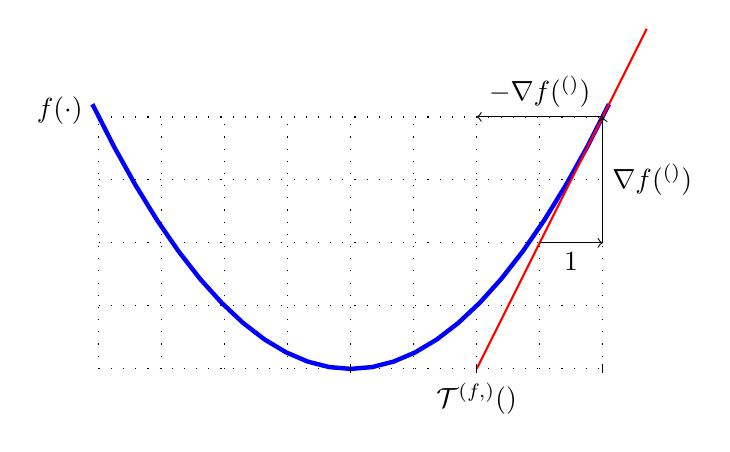
\begin{tikzpicture}[scale=0.8]
					\draw[loosely dotted] (-4,0) grid (4,4);
					\draw[blue, ultra thick, domain=-4.1:4.1] plot (\x,  {(1/4)*\x*\x});
					\draw[red, thick, domain=2:4.7] plot (\x,  {2*\x - 4});
					\draw[<-] (4,4) -- node[right] {$\nabla f(\weights^{(\itercntr)})$} (4,2);
					\draw[->] (4,4) -- node[above] {$-\lrate \nabla f(\weights^{(\itercntr)})$} (2,4);
					\draw[<-] (4,2) -- node[below] {$1$} (3,2) ;
					%\draw[->] (-4.25,0) -- (4.25,0) node[right] {$a$};
					\node[left] at (-4.1, 4.1) {$f(\cdot)$}; 
					\draw[shift={(0,0)}] (0pt,2pt) -- (0pt,-2pt) node[below] {$\overline{\weights}$};
					\draw[shift={(4,0)}] (0pt,2pt) -- (0pt,-2pt) node[below] {$\weights$};
					\draw[shift={(2,0)}] (0pt,2pt) -- (0pt,-2pt) node[below] {$\mathcal{T}^{(f,\lrate)}(\weights)$};
				\end{tikzpicture}
			\end{center}
			\caption{The basic \gls{gradient} step \eqref{equ_def_gd_basic_dict} maps a given \gls{vector} $\weights$ 
			to the updated \gls{vector} $\weights'$. It defines an operator 
			$\mathcal{T}^{(f,\lrate)}(\cdot): \mathbb{R}^{\nrfeatures} \rightarrow \mathbb{R}^{\nrfeatures}:
			 \weights \mapsto \widehat{\weights}$.}
			\label{fig_basic_GD_step_single_dict}
		\end{figure}
		Note that the \gls{gradient} step \eqref{equ_def_gd_basic_dict} optimizes locally—in a \gls{neighborhood} whose size is 
		determined by the \gls{stepsize} $\lrate$—a linear approximation 
		to the \gls{function} $f(\cdot)$. A natural \gls{generalization} of \eqref{equ_def_gd_basic_dict} is to locally 
		optimize the \gls{function} itself—instead of its linear approximation—such that
		\begin{align} 
		\label{equ_approx_gd_step_dict}
		\widehat{\weights} = \argmin_{\weights' \in \mathbb{R}^{\dimlocalmodel}} f(\weights')\!+\!\frac{1}{\lrate}\normgeneric{\weights-\weights'}{2}^2. 
		\end{align}
		We intentionally use the same symbol $\lrate$ for the \gls{parameter} in \eqref{equ_approx_gd_step_dict} 
		as we used for the \gls{stepsize} in \eqref{equ_def_gd_basic_dict}. The larger the $\lrate$ we choose in 
		\eqref{equ_approx_gd_step_dict}, the more progress the update will make toward reducing the 
		\gls{function} value $f(\widehat{\weights})$. Note that, much like the \gls{gradient} step \eqref{equ_def_gd_basic_dict}, 
		the update \eqref{equ_approx_gd_step_dict} also defines an operator 
		that is parameterized by the \gls{function} $f(\cdot)$ and the \gls{learnrate} $\lrate$. For a \gls{convex} \gls{function}  
		$f(\cdot)$, this operator is known as the \gls{proxop} of $f(\cdot)$ \cite{ProximalMethods}. 
					\\ 
		See also: \gls{differentiable}, \gls{function}, \gls{vector}, \gls{gradient}, \gls{stepsize}, \gls{neighborhood}, \gls{generalization}, \gls{parameter}, \gls{learnrate}, \gls{convex}, \gls{proxop}.},
	first={gradient step},
	firstplural={gradient steps},
	plural={gradient steps},
	text={gradient step}
}

\newglossaryentry{operator} 
{name={operator}, 
	description={An\index{operator} operator is a \gls{function} 
	          with \gls{domain} and \gls{co-domain} having a specific 
			  mathematical structure such as a \gls{vectorspace}, \gls{hilbertspace}
			  or a \gls{metricspace} \cite{Bauschke:2017,DunfordSchwartz1988}. 
			  Many \gls{ml} methods involve operators with \gls{domain} and \gls{co-domain} 
			  being an \gls{euclidspace}.
							\\ 
		See also: \gls{vectorspace}, \gls{function}, \gls{hilbertspace}.},
	first={operator},
	type=math, 
	plural={operators},
	firstplural={operators},
	text={operator}
}

\newglossaryentry{contractop}
{name={contraction operator},
	description={An\index{contraction operator} operator 
	   $\fixedpointop: \mathbb{R}^{\nrfeatures} \rightarrow \mathbb{R}^{\nrfeatures}$
		is a contraction if, for some $\contractfac \in [0,1)$,
		\begin{equation} 
			\nonumber
			\normgeneric{ \fixedpointop \weights\!-\!\fixedpointop \weights'}{2}  \leq  \contractfac	\normgeneric{\weights\!-\!\weights'}{2} \mbox{ holds for any } \weights,\weights' \in \mathbb{R}^{\nrfeatures}.
		\end{equation}
	},
	first={contraction operator},
	text={contraction operator}, 
	firstplural={contraction operators}, 
	plural={contraction operators}
}
	

\newglossaryentry{proxop}
{name={proximal operator},
	description={Given\index{proximal operator} a \gls{convex} 
		\gls{function} $f(\weights')$, we define its proximal operator as \cite{Bauschke:2017}, \cite{ProximalMethods}  
		$$\proximityop{f(\cdot)}{\weights}{\rho}\defeq \argmin_{\weights' \in \mathbb{R}^{\dimlocalmodel}} \bigg[ f(\weights')\!+\!\frac{\rho}{2} \normgeneric{\weights- \weights'}{2}^{2}\bigg] \mbox{ with } \rho > 0. $$ 
		As illustrated in Fig. \ref{fig_proxoperator_opt_dict}, evaluating the proximal operator 
		amounts to minimizing a penalized variant of $f(\weights')$. The penalty term is the 
		scaled squared Euclidean distance to a given \gls{vector} $\weights$ (which is the input to the proximal operator). 
		The proximal operator can be interpreted as a \gls{generalization} of the \gls{gradstep}, which is defined 
		for a \gls{smooth} \gls{convex} \gls{function} $f(\weights')$. Indeed, taking a 
		\gls{gradstep} with \gls{stepsize} $\lrate$ at the current \gls{vector} $\weights$ 
		is the same as applying the proximal operator of the \gls{function} $\tilde{f}(\weights')= \big( \nabla f(\weights)\big)\,^{T} (\weights'-\weights)$ 
		and using $\rho=1/\lrate$.
			\begin{figure}[H]
			\begin{center}
				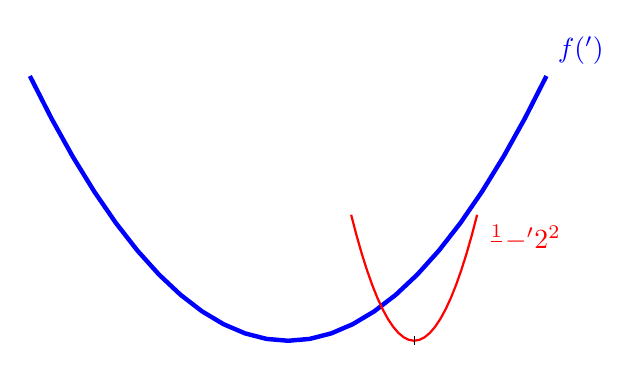
\begin{tikzpicture}[scale=0.8]
					% Original quadratic function
					\draw[blue, ultra thick, domain=-4.1:4.1] plot (\x, {(1/4)*\x*\x}) node[above right] {$f(\weights')$};		
					% Quadratic function with larger curvature, centered at w = 2
					\draw[red, thick, domain=1:3] plot (\x, {2*(\x - 2)*(\x - 2)}) node[below right] {$\frac{1}{\lrate}\normgeneric{\weights-\weights'}{2}^{2}$};
					% Axes
					% Minimum point of second curve
					\draw[shift={(2,0)}] (0pt,2pt) -- (0pt,-2pt) node[below] {$\weights$};
					%\node at (2,0.5) [anchor=north] {$\weights$};
				\end{tikzpicture}
			\end{center}
			\caption{The proximal operator updates a \gls{vector} $\weights$ by minimizing a penalized version 
				of the \gls{function} $f(\cdot)$. The penalty term is the scaled squared Euclidean distance between the optimization 
				variable $\weights'$ and the given \gls{vector} $\weights$.	\label{fig_proxoperator_opt_dict}}
		\end{figure}
		See also: \gls{convex}, \gls{function}, \gls{vector}, \gls{generalization}, \gls{gradstep}, \gls{smooth}, \gls{stepsize}.},
	first={proximal operator},
	text={proximal operator}
}

\newglossaryentry{proximable}
{name={proximable},
	description={A\index{proximable} 
		\gls{convex} \gls{function} for which the \gls{proxop} can be computed efficiently is 
		sometimes referred to as proximable or simple \cite{Condat2013}.
					\\ 
		See also: \gls{convex}, \gls{function}, \gls{proxop}.},
	first={proximable},
	text={proximable}
}


\newglossaryentry{connected}
{name={connected}, 
	description={An\index{connected} 
	    \gls{undirectedgraph} $\graph=\pair{\nodes}{\edges}$ is 
		connected if for every 
		non-empty subset $\nodes' \subset \nodes$ we can find at least one edge 
		connecting a node in $\nodes'$ with some node in $\nodes \setminus \nodes'$.
		\begin{figure}[H]
		\centering
	\begin{tikzpicture}
	% Horizontal axis
	% Left graph (single edge)
	\node[circle, fill=black, inner sep=1.5pt, label=above:{1}] (A1) at (0, 1.5) {};
	\node[above=0.5cm of A1, align=center] {not connected};
	\node[circle, fill=black, inner sep=1.5pt, label=below right:{2}] (B1) [below right=0.8cm and 0.5cm of A1] {};
	\node[circle, fill=black, inner sep=1.5pt, label=below left:{3}] (C1) [below left=0.8cm and 0.5cm of A1] {};
	\draw [line width=1 pt]  (A1) -- (B1);
	% Middle graph (two edges, shifted right)
	\begin{scope}[xshift=3.5cm]
		\node[circle, fill=black, inner sep=1.5pt, label=above:{1}] (A2) at (0, 1.5) {};
		\node[above=0.5cm of A2, align=center] {connected};
		\node[circle, fill=black, inner sep=1.5pt, label=below right:{2}] (B2) [below right=0.8cm and 0.5cm of A2] {};
		\node[circle, fill=black, inner sep=1.5pt, label=below left:{3}] (C2) [below left=0.8cm and 0.5cm of A2] {};
		\draw [line width=1 pt]  (A2) -- (B2);
		\draw [line width=1 pt]  (B2) -- (C2);
	\end{scope}
\end{tikzpicture}
\end{figure} 
		See also: \gls{undirectedgraph}, \gls{algconn}.}, 
	type=math, 
	first={connected},
	text={connected}
}
	
	
\newglossaryentry{mvndist}
{name={multivariate normal distribution}, 
	description={The\index{multivariate normal distribution} multivariate normal distribution, 
		which is denoted by $\mvnormal{\meanvecgeneric}{\covmtxgeneric}$, is a fundamental 
		\gls{probmodel} for numerical \glspl{featurevec} of fixed dimension $\nrfeatures$. 
		It defines a family of \glspl{probdist} over \gls{vector}-valued \glspl{rv} 
		$\featurevec \in \mathbb{R}^{\nrfeatures}$~\cite{BertsekasProb}, \cite{GrayProbBook}, \cite{Lapidoth09}. 
		Each distribution in this family is fully specified by its \gls{mean} \gls{vector} 
		$\meanvecgeneric \in \mathbb{R}^{\nrfeatures}$ and \gls{covmtx} 
		$\covmtxgeneric \in \mathbb{R}^{\nrfeatures \times \nrfeatures}$. When the 
		\gls{covmtx} $\covmtxgeneric$ is invertible, the corresponding \gls{probdist} is 
		characterized by the following \gls{pdf}:
		\[p(\featurevec) = 
 		\frac{1}{\sqrt{(2\pi)^{\nrfeatures} \det\,(\covmtxgeneric)}} 
 		\exp\left[ -\frac{1}{2} 
 		(\featurevec - \meanvecgeneric)\,^{T}\, \covmtxgeneric^{-1} 
 		(\featurevec - \meanvecgeneric) \right].
 		\]
		Note that this \gls{pdf} is only defined when $\covmtxgeneric$ is invertible.
   		More generally, any \gls{rv} $\featurevec \sim \mvnormal{\meanvecgeneric}{\covmtxgeneric}$ 
   		admits the following representation:
  		\[
    		\featurevec = \mA \vz + \meanvecgeneric
   		\]
   		where $\vz \sim \mvnormal{\mathbf{0}}{\mathbf{I}}$ is a \gls{stdnormvec} 
   		and $\mA \in \mathbb{R}^{\nrfeatures \times \nrfeatures}$ satisfies $\mA \mA^\top = \covmtxgeneric$. 
   		This representation remains valid even when $\covmtxgeneric$ is singular, in which case $\mA$ 
   		is not full rank~\cite[Ch. 23]{Lapidoth2017}.
   		The family of multivariate normal distributions is exceptional among \glspl{probmodel} for numerical 
   		quantities, at least for the following reasons. First, the family is closed under affine 
   		transformations, i.e.,
		\[ 
		\featurevec \sim \mathcal{N}(\meanvecgeneric,\covmtxgeneric) \mbox{ implies } 
		\mB\featurevec\!+\!\vc \sim \mathcal{N}\big( \mB\meanvecgeneric+\vc,\mB \covmtxgeneric \mB\,^{T} \big). 
		\]
		Second, the \gls{probdist} $\mathcal{N}(\mathbf{0},\covmtxgeneric)$ maximizes the 
		\gls{diffentropy} among all distributions with the same \gls{covmtx} $\covmtxgeneric$~\cite{coverthomas}. 
		\\ 
		See also: \gls{probmodel}, \gls{probdist}, \gls{stdnormvec}, \gls{diffentropy}, \gls{gaussrv}.}, 
	first={multivariate normal distribution},
	text={multivariate normal distribution}
}

\newglossaryentry{stdnormvec}
{name={standard normal vector}, 
	description={A\index{standard normal vector} standard normal \gls{vector} is a random 
		\gls{vector} $\vx=\big(x_{1}, \,\ldots, \,x_{\nrfeatures}\big)\,^{T}$ 
		whose entries are \gls{iid} \glspl{gaussrv} $x_{\featureidx} \sim \mathcal{N}(0,1)$. 
		It is a special case of a \gls{mvndist}, $\vx \sim \mathcal(\mathbf{0},\mathbf{I})$.
		\\ 
		See also: \gls{vector}, \gls{iid}, \gls{gaussrv}, \gls{mvndist}, \gls{rv}.}, 
	first={standard normal vector},
	text={standard normal vector}
}

\newglossaryentry{earlystopping}
{name={early stopping}, 
	description={Consider an \gls{erm}-based method that uses an 
	iterative \gls{optmethod} (such as \gls{gd}) to learn \glspl{modelparam} 
	via minimizing the \gls{emprisk} on a given \gls{trainset}.
	Early stopping \index{early stopping} refers to terminating the iterations 
	even if they still substantially decrease the \gls{emprisk} on the 
	\gls{trainset}. Instead of monitoring the \gls{objfunc} (which is the 
	\gls{emprisk} on the \gls{trainset}), early stopping monitors the \gls{valerr} 
	incurred by the \glspl{modelparam} in each iteration. Early stopping can be 
	interpreted as an implementation of \gls{regularization} via \gls{model} 
	pruning. Indeed, terminating an iterative \gls{optmethod} after a small number 
	of iterations restricts the set of \glspl{modelparam} that can be reached from the 
	initialization (see Fig.\ \ref{fig_early_stopping_dict}).
	\begin{figure}[htbp]
	\centering
		\begin{tikzpicture}[>=Stealth, scale=2]
		% Initialization
		\fill (0,0) circle (0.6pt) node[above] {\small $\weights^{(0)}$};
		\node at (-0.4,0) {\small $\hypospace^{(1)}$};
		\node at (-1.2,0) {\small $\hypospace^{(2)}$};
			\node at (-2,0) {\small $\hypospace \ldots$};
		% T-step reachable sets (early stopping = smaller T)
		\draw[densely dotted] (0,0) ellipse (0.8 and 0.4);
		\draw[dashed] (0,0) ellipse (1.6 and 0.8);
		% Example gradient path (just illustrative)
		\draw[->] (0,0) -- (0.8,0.) node [pos=0.6,above] {\tiny $1$ step};
		\draw[->] (0.0,0.0) -- (0,-0.8) node [pos=0.9,right] {\tiny $2$ steps};
		\end{tikzpicture}
		\caption{A \gls{gdmethod} for \gls{erm} using a \gls{hypospace} $\hypospace$ 
		    defines a nested \gls{sequence} of effective \glspl{hypospace} 
			$\hypospace^{(1)} \subseteq \hypospace^{(2)} \subseteq \ldots \subseteq \hypospace$. 
			The effective \gls{hypospace} $\hypospace^{(\iteridx)}$ is 
		    determined by all \glspl{modelparam} that can be reached from the initialization 
			$\weights^{(0)}$ within $\iteridx$ \glspl{gradstep}. \label{fig_early_stopping_dict}}
		\end{figure} \\ 
		See also: \gls{gdmethod}, \gls{regularization}, \gls{overfitting}.},
	first={early stopping},
	text={early stopping}
}

\newglossaryentry{statasp}
{name={statistical aspects}, 
	description={By statistical aspects\index{statistical aspects} 
		of an \gls{ml} method, we refer to (properties of) the \gls{probdist} of its output 
		under a \gls{probmodel} for the \gls{data} fed into the method.
					\\ 
		See also: \gls{ml}, \gls{probdist}, \gls{probmodel}, \gls{data}.},
	first={statistical aspects},
	text={statistical aspects}
}

\newglossaryentry{compasp}
{name={computational aspects}, 
	description={By computational 
		aspects\index{computational aspects} of an \gls{ml} method, we mainly refer to the computational 
		resources required for its implementation. For example, if an \gls{ml} method uses iterative 
		optimization techniques to solve \gls{erm}, then its computational aspects include: 1) how 
		many arithmetic operations are needed to implement a single iteration (i.e., a \gls{gradstep}); 
		and 2) how many iterations are needed to obtain useful \glspl{modelparam}. One important 
		example of an iterative optimization technique is \gls{gd}.
					\\ 
		See also: \gls{ml}, \gls{erm}, \gls{gradstep}, \glspl{modelparam}, \gls{gd}.}, 
	first={computational aspects},
	text={computational aspects}
}

\newglossaryentry{zerooneloss}
{name={$\bf 0/1$ loss},
sort={zerooneloss}, 
	description={The $0/1$ \gls{loss}\index{$0/1$ loss} $\lossfunczo{\pair{\featurevec}{\truelabel}}{\hypothesis}$ 
		measures the quality of a \gls{classifier} $\hypothesis(\featurevec)$ that delivers a 
		\gls{prediction} $\predictedlabel$ (e.g., via thresholding \eqref{equ_def_threshold_bin_classifier_dict}) 
		for the \gls{label} $\truelabel$ of a \gls{datapoint} with \glspl{feature} $\featurevec$. It is equal to $0$ if 
		the \gls{prediction} is correct, i.e., 
		$\lossfunczo{\pair{\featurevec}{\truelabel}}{\hypothesis}=0$ when $\predictedlabel=\truelabel$. It is 
		equal to $1$ if the \gls{prediction} is wrong, i.e., $\lossfunczo{\pair{\featurevec}{\truelabel}}{\hypothesis}=1$ 
		when $\predictedlabel\neq\truelabel$.
				\\ 
		See also: \gls{loss}, \gls{classifier}, \gls{prediction}, \gls{label}, \gls{datapoint}, \gls{feature}.},
    	first={$0/1$ loss},
	text={$0/1$ loss}
}

\newglossaryentry{probability}
{name={probability}, 
	description={We\index{probability} assign a probability value, typically chosen in the 
		interval $[0,1]$, to each \gls{event} that can occur in a \gls{randomexperiment}  
		\cite{BillingsleyProbMeasure}, \cite{BertsekasProb}, \cite{HalmosMeasure},  \cite{KallenbergBook}.
		\\
		See also: \gls{event}, \gls{randomexperiment}. },
	first={probability},
	firstplural={probabilities},
	plural={probabilities},
	text={probability}
}
	
\newglossaryentry{underfitting}
{name={underfitting},
	description={Consider\index{underfitting} 
		an \gls{ml} method that uses \gls{erm} to learn a \gls{hypothesis} with the \gls{minimum} \gls{emprisk} 
		on a given \gls{trainset}. Such a method is underfitting the \gls{trainset} if it is 
		not able to learn a \gls{hypothesis} with a sufficiently low \gls{emprisk} on the \gls{trainset}. 
		If a method is underfitting, it will typically also not be able to learn a \gls{hypothesis} with 
		a low \gls{risk}.
					\\ 
		See also: \gls{ml}, \gls{erm}, \gls{hypothesis}, \gls{minimum}, \gls{emprisk}, \gls{trainset}, \gls{risk}.},
	first={underfitting},
	text={underfitting}
}

\newglossaryentry{overfitting}
{name={overfitting},
	description={Consider\index{overfitting} an 
		\gls{ml} method that uses \gls{erm} to learn a \gls{hypothesis} with the \gls{minimum} \gls{emprisk} on 
		a given \gls{trainset}. Such a method is overfitting the \gls{trainset} if it learns 
		a \gls{hypothesis} with a low \gls{emprisk} on the \gls{trainset} but a significantly higher \gls{loss} outside the \gls{trainset}.
					\\ 
		See also: \gls{erm}, \gls{generalization}, \gls{validation}, \gls{gengap}.},
	first={overfitting},
	text={overfitting}
}

\newglossaryentry{gdpr}
{name={general data protection regulation (GDPR)},
	description={The\index{general data protection regulation (GDPR)} GDPR
			was enacted by the European Union (EU), effective from 25 May 2018 \cite{GDPR2016}. 
			It safeguards the privacy and \gls{data} rights of individuals in the EU. 
			The GDPR has significant implications for how \gls{data} are collected, stored, and used in \gls{ml}  
			applications. Key provisions include the following:
			\begin{itemize}
				\item \Gls{dataminprinc}: \gls{ml} systems should only use the necessary amount of personal 
				\gls{data} for their purpose.
				\item \Gls{transparency} and \gls{explainability}: \gls{ml} systems should enable their users to 
				understand how the systems make decisions that impact the users.
				\item \Gls{data} subject rights: Users should get an opportunity to access, rectify, and delete their personal \gls{data}, as well as to object to automated decision-making and profiling.
				\item Accountability: Organizations must ensure robust \gls{data} security and demonstrate 
				compliance through documentation and regular audits.
			\end{itemize}
		See also: \gls{data}, \gls{ml}, \gls{dataminprinc}, \gls{transparency}, \gls{explainability}.}, 
	first={general data protection regulation (GDPR)},
	text={GDPR}
}

\newglossaryentry{normaldist} 
{name={normal distribution}, 
 description={See\index{normal distribution} \gls{gaussrv}.},
 first={normal distribution}, 
 firstplural={normal distributions},
 plural={normal distributions},
 type=math, 
 text={normal distribution}
}
	
\newglossaryentry{gaussrv}
{name={Gaussian random variable (Gaussian RV)}, 
	plural={Gaussian RVs}, 
	description={A \index{Gaussian random variable (Gaussian RV)} standard Gaussian \gls{rv} is a 
		real-valued \gls{rv} $x$ with \gls{pdf} \cite{BertsekasProb}, \cite{GrayProbBook}, \cite{papoulis}
		\begin{equation}
			\nonumber
			p(x) = \frac{1}{\sqrt{2\pi}} \exp\,(-x^2/2). 
		\end{equation}
		Given a standard \gls{gaussian} \gls{rv} $x$, we can construct a general \gls{gaussian} 
		\gls{rv} $x'$ with \gls{mean} $\mu$ and \gls{variance} $\sigma^2$ via $x' \defeq \sigma x + \mu$. 
		The \gls{probdist} of a \gls{gaussian} \gls{rv} is referred to as normal 
		distribution, denoted by $\mvnormal{\mu}{\sigma^{2}}$. 
		\\ 
		A \gls{gaussian} random \gls{vector} $\featurevec \in \mathbb{R}^{\featuredim}$ with 
		\gls{covmtx} $\mathbf{C}$ and \gls{mean} ${\bm \mu}$ can be constructed as \cite{GrayProbBook}, \cite{papoulis}, \cite{Lapidoth09}
		\[
		\featurevec \defeq \mathbf{A} \vz + {\bm \mu}
		\]
		where $\vz \defeq \big( z_{1}, \,\ldots, \,z_{\featuredim} \big)\,^{T}$ is a \gls{vector} 
		of \gls{iid} standard Gaussian \glspl{rv}, and $\mA \in \mathbb{R}^{\featuredim \times \featuredim}$ is any \gls{matrix} satisfying $\mA \mA\,^{T} = \mC$. 
		The \gls{probdist} of a Gaussian random \gls{vector} is referred to as the \gls{mvndist}, 
		denoted by $\mvnormal{\bm \mu}{\mathbf{C}}$.
		\\
		We can interpret a \gls{gaussian} random \gls{vector} $\featurevec=\big(\feature_{1},\,\ldots,\,\feature_{\nrfeatures}\big)$ as a \gls{stochproc} 
		indexed by the set $\mathcal{I}=\{1,\,\ldots,\,\nrfeatures\}$. A \glspl{GaussProc} is a 
		\gls{stochproc} over an arbitray index set $\mathcal{I}$ such that any restriction 
		to a finite subset $\mathcal{I}' \subseteq \mathcal{I}$ yields a \gls{gaussian} 
		random \gls{vector} \cite{Rasmussen2006Gaussian}.
  		\\
        		\Gls{gaussian} \glspl{rv} are widely used \glspl{probmodel} in the 
				statistical analysis of \gls{ml} methods. Their significance arises 
				partly from the \gls{clt} which provides conditions under which 
				the average of many independent \glspl{rv} (not necessarily \gls{gaussian} themselves) 
				tends toward a \gls{gaussian} \gls{rv} \cite{ross2013first}.
		\\ 
		The \gls{mvndist} is also distinct in that it represents \gls{maximum} \gls{uncertainty}. 
		Among all \gls{vector}-valued \glspl{rv} with a given \gls{covmtx} $\mC$, the 
		\gls{rv} $\vx \sim \mvnormal{\bm \mu}{\mathbf{C}}$ maximizes \gls{diffentropy} 
		\cite[Th. 8.6.5]{coverthomas}. This makes \glspl{GaussProc} a natural choice for 
		capturing \gls{uncertainty} or the lack of (domain) knowledge.
		\\ 
		See also: \gls{mvndist}, \gls{GaussProc}, \gls{probmodel}, \gls{clt}, \gls{diffentropy}.},
	first={Gaussian random variable (Gaussian RV)},
	type=math, 
	text={Gaussian RV}
}

\newglossaryentry{gaussian} 
{name={Gaussian}, 
 description={See\index{Gaussian} \gls{gaussrv}.},
 first={Gaussian},
 type=math,
 text={Gaussian}
 }
	
\newglossaryentry{clt}
{name={central limit theorem (CLT)},
	description={Consider a sequence of \gls{iid} \glspl{rv} \( \feature^{(\sampleidx)} \), for \( \sampleidx = 1, \,2, \,\ldots \), 
		each with \gls{mean} zero and finite \gls{variance} \( \sigma^2 > 0 \). 
		The \index{central limit theorem (CLT)} CLT states that the normalized sum 
		\[
		s^{(\samplesize)} \defeq \frac{1}{\sqrt{\samplesize}} \sum_{\sampleidx = 1}^{\samplesize} \feature^{(\sampleidx)} 
		\]
		converges in distribution to a \gls{gaussrv} with \gls{mean} zero and \gls{variance} \( \sigma^2 \) as \( \samplesize \to \infty \) \cite[Proposition~2.17]{AsympVanderVaartBook}.
		One elegant way to derive the CLT is via the \gls{characteristicfunc} of the normalized sum \( s^{(\samplesize)} \). 
		Let $ \phi(t) = \expect \big\{ \exp \big( j t \feature \big) \big\}$ (with the imaginary unit $j = \sqrt{-1}$) 
		be the common \gls{characteristicfunc} of each sum and $\feature^{(\sampleidx)}$, and let \( \phi^{(\samplesize)}(t) \) 
		denote the \gls{characteristicfunc} of \( s^{(\samplesize)} \). Define an operator \( \mathcal{T} \) acting on \glspl{characteristicfunc} 
		such that
		\[
		\phi^{(\samplesize)}(t) = \mathcal{T}(\phi^{(\samplesize-1)})(t) \defeq \phi\left( \frac{t}{\sqrt{\samplesize}} \right) \cdot \phi^{(\samplesize-1)}\left( \frac{\sqrt{\samplesize-1}}{\sqrt{\samplesize}} t \right).
		\]
		This \gls{fixedpointiter} captures the effect of recursively adding an \gls{iid} \gls{rv} $\featurevec^{(\samplesize)}$ 
		and rescaling. Iteratively applying \( \mathcal{T} \) leads to \gls{convergence} of \( \phi^{(\samplesize)}(t) \) toward the fixed point
		\[
		\phi^*(t) = \exp\,(-t^2 \sigma^2 / 2)
		\]
		which is the \gls{characteristicfunc} of a \gls{gaussrv} with \gls{mean} zero and \gls{variance} 
		\( \sigma^2 \). \Glspl{generalization} of the CLT allow for dependent or nonidentically distributed \glspl{rv} \cite[Sec.~2.8]{AsympVanderVaartBook}.
		\begin{figure}[H]
			\centering
			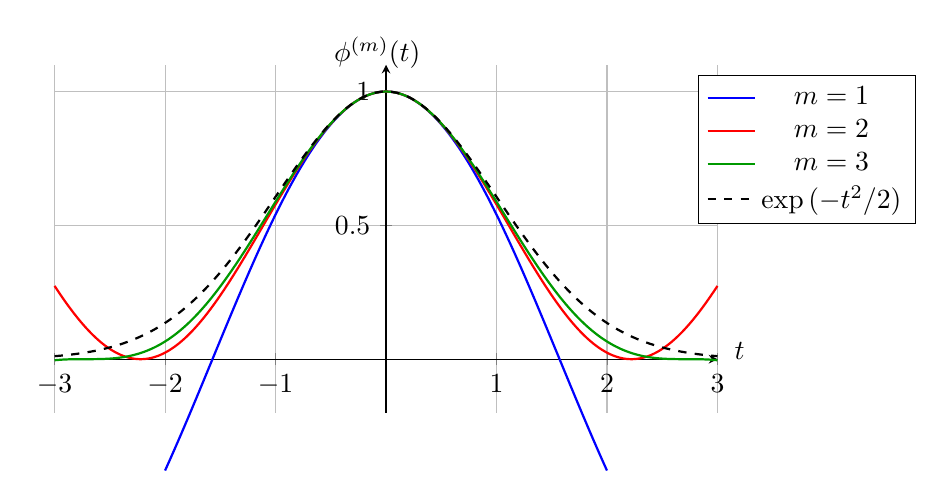
\begin{tikzpicture}
			\begin{axis}[
			width=10cm,
			height=6cm,
			xlabel={},
			ylabel={},
			legend style={at={(0.97,0.97)}, anchor=north west},
			domain=-3:3,
			ylabel style={
			yshift=10pt   % shift label up by 10pt
			},
			samples=400,
			ymin=-0.2, ymax=1.1,
			axis lines=middle,
			clip=false,
			grid=both,
			]
			\addplot[thick, blue,domain=-2:2] {cos(x/sqrt(1) r)^1};
			\addlegendentry{$m=1$}
			\addplot[thick, red] {cos(x/sqrt(2) r)^2};
			\addlegendentry{$m=2$}
			\addplot[thick, green!60!black] {cos(x/sqrt(3) r)^3};
			\addlegendentry{$m=3$}
			\addplot[thick, dashed, black] {exp(-x^2/2)};
			\addlegendentry{$\exp\,(-t^2/2)$}
			\node[anchor=south, rotate=0] at (axis cs:-0.08,1.05) {$\phi^{(m)}(t)$};
			\node[anchor=north, rotate=0] at (axis cs: 3.2,0.1) {$t$};
			\end{axis}
			\end{tikzpicture}
			\caption{\Glspl{characteristicfunc} of normalized sums of \gls{iid} \glspl{rv} $x^{(\sampleidx)} \in \{-1,1\}$ 
			for $\sampleidx=1,\,\ldots,\,\samplesize$ compared to the Gaussian limit.}
		\end{figure}
		See also: \gls{rv}, \gls{gaussrv}.},
	first={central limit theorem (CLT)},
	type=math, 
	text={CLT}
}


\newglossaryentry{GaussProc}
{name={Gaussian process (GP)},
  description={A \index{Gaussian process (GP)}GP is a collection of \glspl{rv} 
  	$\{f(\featurevec)\}_{\featurevec \in \featurespace}$ indexed by input values $\featurevec$ 
  	from some input space $\featurespace$ such that, for any finite subset 
  	$\featurevec^{(1)}, \,\ldots, \,\featurevec^{(\samplesize)} \in \featurespace$, 
  	the corresponding \glspl{rv} $f(\featurevec^{(1)}, \,\ldots, \,\featurevec^{(\samplesize)})$ 
	have a joint \gls{mvndist} 
  	\[
  	f \left( \featurevec^{(1)}, \,\ldots, \,\featurevec^{(\samplesize)} \right) \sim \mathcal{N}(\boldsymbol{\mu}, \mathbf{K}).
  	\]
  	For a fixed input space $\featurespace$, a GP is 
	fully specified (or parameterized) by: 1) a \gls{mean} \gls{function} 
	$\mu(\featurevec) = \expect\{ f(\featurevec)\}$; and 2) 
	a \gls{covariance} \gls{function} $\kernelmap{\featurevec}{\featurevec'}= \expect\{ \big(f(\featurevec)-\mu(\featurevec)\big) \big(f(\featurevec')-\mu(\featurevec')\big) \big\}$.\\
  	{\bf Example.} We can interpret the temperature distribution across Finland (at a specific 
  	point in time) as the \gls{realization} of a GP $f(\featurevec)$, where each input 
	$\featurevec = (\text{lat}, \text{lon})$ denotes a geographic location. Temperature 
	observations from \gls{fmi} weather stations provide values $f(\featurevec)$ at specific 
	locations (see Fig. \ref{fig_gp_FMI_dict}). A GP allows us to predict the temperature 
	nearby \gls{fmi} weather stations and to quantify the \gls{uncertainty} 
  	of these \glspl{prediction}. 
  	\begin{figure}[H]
  	\begin{center}
  		\begin{tikzpicture}
		\begin{axis}[
		axis equal,
		hide axis,
		scale=1.2,
		xmin=17, xmax=32,
		ymin=55, ymax=71,
		%	width=15cm,
		%	height=20cm,
		clip=true
		]
		% --- Finland border (polyline) ---
		\addplot[
		color=black,
		thick
		] table [x=lon, y=lat, col sep=comma] {assets/finland_border.csv};
		% --- FMI sample stations ---
		\addplot[
		only marks,
		mark=*,
		mark options={fill=blue},
		color=black
		] table [x=lon, y=lat, col sep=comma] {assets/fmi_stations_subset.csv};
		% Draw manual axes
		\draw[->, thick] (axis cs:19,59) -- (axis cs:25.5,59) node[anchor=west] {longitude (lon)};
		\draw[->, thick] (axis cs:19,59) -- (axis cs:19,65.5) node[anchor=south] {latitude (lat)};
		\end{axis}
		\end{tikzpicture}
		\vspace*{-15mm}
	\end{center}
	\caption{For a given point in time, we can interpret the current temperature distribution 
	over Finland as a \gls{realization} of a GP indexed by geographic coordinates and 
	sampled at \gls{fmi} weather stations. The weather stations are indicated by blue dots. \label{fig_gp_FMI_dict}}
	\end{figure}
	See also: \gls{mvndist}, \gls{uncertainty}, \gls{gaussrv}.}, 
  first={GP}, 
  type=math, 
  text={GP}
}

\newglossaryentry{trustAI}
{name={trustworthy artificial intelligence (trustworthy AI)},
	description={Besides the \gls{compasp} and \gls{statasp}, a third main design aspect of 
		\gls{ml} methods is their trustworthiness\index{trustworthy artificial intelligence (trustworthy AI)} \cite{pfau2024engineeringtrustworthyaideveloper}. 
		The EU has put forward seven key requirements (KRs) for trustworthy 
		\gls{ai} (which typically build on \gls{ml} methods) \cite{ALTAIEU}: 
	\begin{enumerate}[label=\arabic*)]
		\item KR1 – Human agency and oversight;
		\item KR2 – Technical \gls{robustness} and safety;
		\item KR3 – Privacy and \gls{data} governance;
		\item KR4 – \Gls{transparency};
		\item KR5 – Diversity, non-discrimination and fairness; 
		\item KR6 – Societal and environmental well-being;
		\item KR7 – Accountability. 
	\end{enumerate}
		See also: \gls{compasp}, \gls{statasp}, \gls{ml}, \gls{ai}, \gls{robustness}, \gls{data}, \gls{transparency}.},
	first={trustworthy artificial intelligence (trustworthy AI)},
	text={trustworthy AI}
}

\newglossaryentry{sqerrloss}
{name={squared error loss},
	description={The squared 
		error\index{squared error loss} \gls{loss} measures the \gls{prediction} error of a 
		\gls{hypothesis} $\hypothesis$ when predicting a numeric \gls{label} $\truelabel \in \mathbb{R}$ 
		from the \glspl{feature} $\featurevec$ of a \gls{datapoint}. It is defined as 
		\begin{equation} 
			\nonumber
			\lossfunc{(\featurevec,\truelabel)}{\hypothesis} \defeq \big(\truelabel - \underbrace{\hypothesis(\featurevec)}_{=\predictedlabel} \big)^{2}. 
		\end{equation} 
			\\ 
		See also: \gls{loss}, \gls{prediction}, \gls{hypothesis}, \gls{label}, \gls{feature}, \gls{datapoint}.},
	first={squared error loss},
	text={squared error loss}
}


 \newglossaryentry{projection}
 {name={projection}, 
       description={Consider\index{projection} a subset $\paramspace \subseteq \mathbb{R}^{\dimlocalmodel}$ of 
	   the $\dimlocalmodel$-dimensional \gls{euclidspace}. We define the projection $\projection{\paramspace}{\weights}$
	   of a \gls{vector} $\weights \in \mathbb{R}^{\dimlocalmodel}$ onto $\paramspace$ as
	   \begin{equation} 
   	   	\nonumber
		\label{equ_def_proj_generic_dict}
  	    	\projection{\paramspace}{\weights} = \argmin_{\weights' \in \paramspace} \normgeneric{\weights - \weights'}{2}. 
        	    \end{equation}
	    In other words, $\projection{\paramspace}{\weights}$ is the \gls{vector} in $\paramspace$ 
	    that is closest to $\weights$. The projection is only well defined for subsets $\paramspace$ 
	    for which the above \gls{minimum} exists \cite{BoydConvexBook}.
		 			\\ 
	    See also: \gls{euclidspace}, \gls{vector}, \gls{minimum}.},
	first={projection},
	text={projection}
}


\newglossaryentry{projgd}
{name={projected gradient descent (projected GD)},
	description={Consider an \gls{erm}-based method that uses a parameterized \gls{model} with  
		\gls{paramspace} $\paramspace \subseteq \mathbb{R}^{\dimlocalmodel}$. Even if 
		the \gls{objfunc} of \gls{erm} is \gls{smooth}, we cannot use basic \gls{gd}, as 
		it does not take into account constraints on the optimization variable (i.e., the \glspl{modelparam}). 
		Projected\index{projected gradient descent (projected GD)} \gls{gd} 
		extends basic \gls{gd} to address this issue. 
		A single iteration of projected \gls{gd} consists of first taking a \gls{gradstep} 
		and then projecting the result back onto the \gls{paramspace}. 
		See Fig. \ref{fig_projected_GD_dict} for a visual illustration.
		\begin{figure}[H]
		\begin{center}
			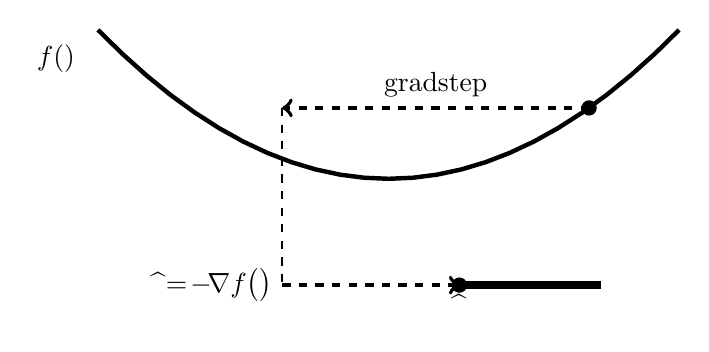
\begin{tikzpicture}[scale=0.9]
			\node [right] at (-5.1,1.7) {$f(\weights)$} ;
			\draw[ultra thick, domain=-4.1:4.1] plot (\x,  {(1/8)*\x*\x});
		%	\draw[dashed, thick, domain=1:3.6] plot (\x,  {\x - 1}) node[right] {$ f\big(\weights^{(\itercntr)}\big)\!+\!\big(\weights\!-\!\weights^{(\itercntr)}\big)^{T} \nabla f\big(\weights^{(\itercntr)}\big)$};
			\draw [fill] (2.83,1) circle [radius=0.1] node[right] {$\weights$};
			\draw[line width =0.5mm,dashed,->] (2.83,1) -- node[midway,above] {\gls{gradstep}} (-1.5,1);
			\draw[line width =0.2mm,dashed] (-1.5,1) --(-1.5,-1.5)  node [below, left]{$\widehat{\weights}=\weights\!-\!\lrate \nabla f\big(\weights\big)$} ;
			\draw[line width =0.5mm,dashed,->] (-1.5,-1.5)  -- node[midway,above] {} (1,-1.5) ; 
			\draw [fill] (1,-1.5) circle [radius=0.1] node[below] {$\projection{\paramspace}{\widehat{\weights}}$};
			\draw[line width=1mm] (1,-1.5) -- (3,-1.5) node[midway, above] {$\paramspace$};
			\end{tikzpicture}
		\vspace*{-5mm}
		\end{center}
		\caption{Projected \gls{gd} augments a basic \gls{gradstep} with a \gls{projection} back 
		onto the constraint set $\paramspace$.}
		\label{fig_projected_GD_dict}
		\end{figure}
		See also: \gls{erm}, \gls{model}, \gls{paramspace}, \gls{objfunc}, \gls{smooth}, \gls{gd}, \glspl{modelparam}, \gls{gradstep}, \gls{projection}.},
	first={projected gradient descent (projected GD)},
	type=math, 
	text={projected GD}
}

\newglossaryentry{diffpriv}
{name={differential privacy (DP)},
  description={Consider\index{differential privacy (DP)} some \gls{ml} method $\algomap$ 
  	that reads in a \gls{dataset} (e.g., the \gls{trainset} 
  	used for \gls{erm}) and delivers some output $\algomap(\dataset)$. The output 
  	could be either the learned \glspl{modelparam} or the \glspl{prediction} for specific \glspl{datapoint}. 
  	DP is a precise measure of \gls{privleakage} incurred by revealing the 
  	output. Roughly speaking, an \gls{ml} method is differentially private if the \gls{probdist} 
  	of the output $\algomap(\dataset)$ remains largely unchanged if the \gls{sensattr} 
  	of one \gls{datapoint} in the \gls{trainset} is changed. Note that DP 
  	builds on a \gls{probmodel} for an \gls{ml} method, i.e., we interpret its output $\algomap(\dataset)$ 
  	as the \gls{realization} of a \gls{rv}. The randomness in the output can be ensured 
  	by intentionally adding the \gls{realization} of an auxiliary \gls{rv} (i.e., adding noise) to 
  	the output of the \gls{ml} method.
				\\ 
	See also: \gls{privleakage}, \gls{sensattr}, \gls{privattack}, \gls{privfunnel}.}, 
  first={DP}, 
  text={DP} 
}

\newglossaryentry{robustness}
{name={robustness},
	description={Robustness\index{robustness} is a key requirement for \gls{trustAI}. It
		refers to the property of an \gls{ml} system to maintain acceptable performance even when 
		subjected to different forms of perturbations. These perturbations may affect the \glspl{feature} 
		of a \gls{datapoint} in order to manipulate the \gls{prediction} delivered by a trained \gls{ml} \gls{model}. 
		Robustness also includes the \gls{stability} of \gls{erm}-based methods against perturbations 
		of the \gls{trainset}. Such perturbations can occur within \gls{datapoisoning} \glspl{attack}. 
		\\ 
		See also: \gls{trustAI},\gls{stability},\gls{datapoisoning}, \gls{attack}.}, 
	first={robustness}, 
	text={robustness} 
}


\newglossaryentry{stability}
{name={stability},
	description={
	Mathematically, a \gls{ml} method is a map $\algomap$ from a given \gls{dataset} $\dataset$ 
	to an output $\algomap(\dataset)$. As a case in point, consider an \gls{erm}-based 
	\gls{ml} method that maps a \gls{trainset} $\dataset$ to the learned \glspl{modelparam} 
	$\algomap(\dataset) = \widehat{\weights}$ which achieve the minimum average \gls{loss} 
	on the \gls{trainset}. Instead of the learned \glspl{modelparam}, the 
	output $\algomap(\dataset)$ could also be the \glspl{prediction} obtained from 
	the trained \gls{model}. Stability\index{stability} refers to the desirable property 
	of $\algomap$ that small changes in the input \gls{dataset} $\dataset$ result in small 
	changes in the output $\algomap(\dataset)$. The notion of stability is intimately related 
	to the notion of \gls{generalization}. In particular, there are formal notions of stability  
	that allow to bound the \gls{gengap} (see \cite[Ch.~13]{ShalevMLBook}).
		To build intuition, consider the three \glspl{dataset} depicted in Fig. \ref{fig_three_data_stability_dict}, each 
		of which is equally likely under the same \gls{data}-generating \gls{probdist}. Since the 
		optimal \glspl{modelparam} are determined by this underlying \gls{probdist}, an accurate 
		\gls{ml} method $\algomap$ should return the same (or very similar) output $\algomap(\dataset)$ 
		for all three \glspl{dataset}. In other words, any useful $\algomap$ must be robust to 
		variability in \gls{sample} \glspl{realization} from the same \gls{probdist}, i.e., it must be stable. 
		\begin{figure}[H]
			\centering
			\begin{tikzpicture}
				\begin{axis}[
				%title={Stem Plots of 3 Datasets},
				    axis lines=none,
					xlabel={$\sampleidx$},
					ylabel={},
					legend pos=north west,
					ymin=0, ymax=10,
					xtick={1,2,3,4,5},
				%	ymajorgrids=true,
					grid style=dashed,
					every axis plot/.append style={very thick}
					]
					% Dataset 1
					\addplot+[only marks,mark=*] coordinates {
						(1,2) (2,4) (3,3) (4,5) (5,7)
					};
				%	\addlegendentry{$\dataset^{(*)}$}
					% Dataset 2
					\addplot+[only marks,mark=square*] coordinates {
						(1,3) (2,2) (3,6) (4,4) (5,5)
					};
				%	\addlegendentry{$\dataset^{(\square)}$}
					% Dataset 3
					\addplot+[only marks,mark=triangle*] coordinates {
						(1,5) (2,7) (3,4) (4,6) (5,3)
					};
				%	\addlegendentry{$\dataset^{(\triangle)}$}
				\end{axis}
			\end{tikzpicture}
			\caption{Three \glspl{dataset} $\dataset^{(*)}$, $\dataset^{(\square)}$, 
			and $\dataset^{(\triangle)}$, each sampled independently from the same 
			\gls{data}-generating \gls{probdist}. A stable \gls{ml} method should return 
			similar outputs when trained on any of these \glspl{dataset}. \label{fig_three_data_stability_dict}}
		\end{figure}
		See also: \gls{generalization}, \gls{robustness}.}, 
	first={stability}, 
	text={stability} 
}

\newglossaryentry{privprot}
{name={privacy protection},
     description={Consider\index{privacy protection} some \gls{ml} method $\algomap$ that reads 
	 	in a \gls{dataset} $\dataset$ and delivers some output $\algomap(\dataset)$. The output 
	 	could be the learned \glspl{modelparam} $\widehat{\weights}$ or the \gls{prediction} 
	 	$\learnthypothesis(\featurevec)$ obtained for a specific \gls{datapoint} with \glspl{feature} 
	 	$\featurevec$. Many important \gls{ml} applications involve \glspl{datapoint} 
		representing humans. Each \gls{datapoint} is characterized by \glspl{feature} $\featurevec$, 
		potentially a \gls{label} $\truelabel$, and a \gls{sensattr} $\sensattr$ (e.g., a recent medical diagnosis). 
		Roughly speaking, privacy protection means that it should be impossible to infer, from the output $\algomap(\dataset)$, 
		any of the \glspl{sensattr} of \glspl{datapoint} in $\dataset$. Mathematically, privacy protection requires non-invertibility 
		of the \gls{map} $\algomap(\dataset)$. In general, just making $\algomap(\dataset)$ non-invertible 
		is typically insufficient for privacy protection. We need to make $\algomap(\dataset)$ sufficiently non-invertible. 
					\\ 
		See also: \gls{ml}, \gls{dataset}, \glspl{modelparam}, \gls{prediction}, \gls{datapoint}, \gls{feature}, \gls{label}, \gls{sensattr}, \gls{map}.}, 
	first={privacy protection}, 
	text={privacy protection} 
}

\newglossaryentry{privleakage}
{name={privacy leakage},
	description={Consider\index{privacy leakage} an \gls{ml} application that processes a 
		\gls{dataset} $\dataset$ and delivers some output, such as the \glspl{prediction} 
		obtained for new \glspl{datapoint}. Privacy leakage arises 
		if the output carries information about a private (or sensitive) \gls{feature} of 
		a \gls{datapoint} of $\dataset$ (such as a human). Based on a \gls{probmodel} 
		for the \gls{data} generation, we can measure the privacy leakage via the \gls{mutualinformation} 
		between the output and the sensitive \gls{feature}. Another quantitative measure of privacy leakage 
		is \gls{diffpriv}. The relations between different measures of privacy leakage have been 
		studied in the literature (see \cite{InfThDiffPriv}). 
				\\ 
		See also: \gls{mutualinformation}, \gls{diffpriv}, \gls{privattack}, \gls{gdpr}. }, 
	first={privacy leakage}, 
	text={privacy leakage} 
}


\newglossaryentry{probmodel}
{name={probabilistic model}, plural={probabilistic models},
	description={A probabilistic \gls{model}\index{probabilistic model} interprets the 
	             generation of \glspl{datapoint} as \glspl{rv} with a joint \gls{probdist}. 
				This joint \gls{probdist} typically involves \glspl{parameter} that have to 
				be manually chosen or learned via statistical inference methods such as 
				\gls{maxlikelihood} estimation \cite{LC}.
					\\ 
		See also: \gls{model}, \gls{datapoint}, \gls{realization}, \gls{rv}, \gls{probdist}, \gls{parameter}, \gls{maxlikelihood}. }, 
	first={probabilistic model}, 
	type=math,
	text={probabilistic model} 
}


\newglossaryentry{mean}
{name={mean}, plural={means},
	description={The \index{mean} mean of a \gls{rv} $\featurevec$, which takes 
 		on values in a \gls{euclidspace} $\mathbb{R}^{\dimlocalmodel}$, is its 
 		\gls{expectation} $\expect\{\featurevec\}$. It is defined as the Lebesgue 
 		integral of $\featurevec$ with respect to the underlying \gls{probdist} $P$ (e.g., 
		see \cite{RudinBookPrinciplesMatheAnalysis} or \cite{BillingsleyProbMeasure}), i.e.,
		\[
			\expect\{\featurevec\} = \int_{\mathbb{R}^{\dimlocalmodel}} \vx \, \mathrm{d}P(\vx).
		\]  
		We also use the term to refer to the average of a finite \gls{dataset}
		$\dataset = \left\{ \vx^{(1)}, \,\ldots, \,\vx^{(\samplesize)} \in \mathbb{R}^{\dimlocalmodel}\right\}$. 
		However, these two definitions are essentially the same. Indeed, we can use 
		a \gls{dataset} to construct a discrete \gls{rv} $\widetilde{\vx}^{(\dataset)}=\vx^{(I)}$ on 
		the \gls{samplespace} $\{1, \,\ldots, \,\samplesize\}$. Here, the index $I$ is 
		chosen uniformly at random, $\prob{I=\sampleidx}=1/\samplesize$ for all 
		$\sampleidx=1,\ldots,\samplesize$. The mean of $\widetilde{\vx}^{(\dataset)}$ is 
		precisely the average $({1}/{\samplesize}) \sum_{\sampleidx=1}^{\samplesize} \vx^{(\sampleidx)}$.
		For a \gls{rv} with finite second-order moment, i.e., 
		$\expect\{ \normgeneric{\featurevec}{2}^{2} \}$ is well-defined and fnite, 
		the mean is characterized as the solution of the 
		following \gls{risk} minimization problem \cite{BertsekasProb}:
		\[
			\expect\{\featurevec\} = \argmin_{\vc \in \mathbb{R}^{\nrfeatures}} 
			\expect \big\{\normgeneric{\featurevec - \vc}{2}^{2}\big \}.
		\]
		For the \gls{rv} $\widetilde{\vx}^{(\dataset)}$, associated with a \gls{dataset}, 
		this \gls{optproblem} reduces to \gls{erm} with \gls{sqerrloss} on $\dataset$. 
		\\ 
		See also: \gls{rv}, \gls{expectation}, \gls{probdist}, \gls{erm}.}, 
	first={mean}, 
	type=math,
	text={mean} 
}

\newglossaryentry{median}
{name={median}, 
plural={medians},
	description={A\index{median} median $\med\,(x)$ of a real-valued \gls{rv} $x$ 
 		is any number $M \in \mathbb{R}$ such that $\prob{ x \leq M} \geq 1/2$ and 
		$\prob{ x \geq M} \geq 1/2$ 
		(see Fig. \ref{fig_median1_dict}) \cite{LC}. 
 		\begin{figure}[H]
			\begin{center}
			\begin{tikzpicture}
 			\begin{axis}[
    			axis lines=middle,
    			xlabel={},
    			ylabel={},
    			ymin=0, ymax=1.1,
    			xmin=-2, xmax=6,
    			xtick=\empty,
    			ytick={0,1/2,1},
    			domain=-2:6,
    			samples=200,
    			width=10cm,
    			height=6cm,
    			smooth,
    			enlargelimits=true,
    			clip=false
  			]
    			% Shifted sigmoid CDF
			\addplot[thick, blue, name path=cdf] {1/(1 + exp(-(x - 1)))} node[pos=0.5, above, yshift=15pt] {$\prob{x \leq \eta}$};    % Vertical and horizontal ruler at F(x) = 0.5
    			\draw[dashed, gray] (axis cs:1,0) -- (axis cs:1,0.5); % vertical
    			\draw[dashed, gray] (axis cs:-2,0.5) -- (axis cs:1,0.5); % horizontal
    			% Mark the median point
   			\filldraw[red] (axis cs:1,0.5) circle (2pt);
  		    \node[below] at (axis cs:1,0) {$M$};
			\node[above right] at (axis cs:6.3,0) {$\eta$};
    			% Label next to curve
  			\end{axis}
			\end{tikzpicture} 
			\end{center}
			\caption{The median of a real-valued \gls{rv} is any number $M$ 
			that partitions $\mathbb{R}$ into two rays with equal \gls{probability}. \label{fig_median1_dict}}
 		\end{figure}  
 		We can define the median $\med\,(\dataset)$ 
 		of a \gls{dataset} $\dataset = \{ x^{(1)}, \,\ldots, \,x^{(\samplesize)} \in \mathbb{R} \}$ 
 		via a specific \gls{rv} $\tilde{x}^{(\dataset)}$ that is naturally associated with $\dataset$. 
 		In particular, this \gls{rv} is defined on the \gls{samplespace} $\{1, \,\ldots, \,\samplesize\}$ 
		via $\tilde{x}^{(\dataset)} \defeq x^{(I)}$. Here, the index $I$ is chosen uniformly 
		at random, i.e., $\prob{I = \sampleidx}=1/\samplesize$ for 
 		all $\sampleidx=1, \,\ldots, \,\samplesize$. If the \gls{rv} $x$ is integrable, any 
		median of $x$ solves the \gls{optproblem}: 
 		$$\min_{x' \in \mathbb{R}} \expect{|x - x'|}.$$ 
		For a the above \gls{rv} $\tilde{x}$ (constructed from a \gls{dataset} $\dataset$), 
		this \gls{optproblem} is \gls{erm} on $\dataset$ using \gls{abserr}. 
 		Like the \gls{mean}, the median of a \gls{dataset} $\dataset$ can also be used 
 		to estimate \glspl{parameter} of an underlying \gls{probmodel}. Compared 
 		with the \gls{mean}, the median is more robust to \glspl{outlier}. For example, 
 		a median of a \gls{dataset} $\dataset$ with more than one \gls{datapoint} does not 
 		change even if we arbitrarily increase the largest element of $\dataset$ (see Fig. \ref{fig_median2_dict}). 
		In contrast, the \gls{mean} will increase arbitrarily.
		\begin{figure}[H]
		\centering
		\begin{tikzpicture}[scale=0.7, y=0.5cm, x=0.5cm]
			\begin{scope}
				\foreach \x/\y in {
					1/2, 4/3, 7/4
				} {
					\draw[dashed, gray] (\x, 0) -- (\x, \y);
					\filldraw[blue] (\x, \y) circle (2pt);
					\node[circle, inner sep=0pt] (ptA\x) at (\x, \y) {};
				}
				\draw[dashed, thick] (0.5, 3) -- (10.5, 3) node[right] {$\med\,(\dataset)\!=\!{\rm mean}(\dataset)$};
				\node at (7.5, -4) {(a)};
			\end{scope}
			\begin{scope}[xshift=12cm]
				\foreach \x/\y in {
					1/2, 4/3, 7/10
				} {
					\draw[dashed, gray] (\x, 0) -- (\x, \y);
					\filldraw[blue] (\x, \y) circle (2pt);
					\node[circle, inner sep=0pt] (ptB\x) at (\x, \y) {};
				}
				\draw[dashed, thick] (0.5, 7.5) -- (10.5, 7.5) node[right] 
				{${\rm mean}\,\big(\widetilde{\dataset}\big)$};
				\draw[dashed, thick] (0.5, 3) -- (10.5, 3) node[right] 
				{$\med\,\big(\widetilde{\dataset}\big)$};
				\node[above right=2pt and 2pt, red] at (ptB7) {\gls{outlier}};
				\node at (7.5, -4) {(b)};
			\end{scope}
		\end{tikzpicture}
		\caption{The median is robust against \gls{outlier} contamination. (a) Original \gls{dataset} $\dataset$. (b) Noisy 
		\gls{dataset} $\widetilde{\dataset}$ including an \gls{outlier}. \label{fig_median2_dict}}
		\end{figure}
		See also: \gls{mean}, \gls{outlier}, \gls{robustness}, \gls{ladregression}.}, 
	first={median}, 
	type=math,
	text={median} 
}

\newglossaryentry{variance}
{name={variance},
	description={The\index{variance} variance of a real-valued \gls{rv} $\feature$ is defined 
	   as the \gls{expectation} $\expect\big\{ \big( x - \expect\{x \} \big)^{2} \big\}$ of 
	   the squared difference between $\feature$ and its \gls{expectation} $\expect\{x \}$. 
	   We extend this definition to \gls{vector}-valued \glspl{rv} $\featurevec$ 
	   as $\expect\big\{ \big\| \featurevec - \expect\{\featurevec \} \big\|_{2}^{2} \big\}$.
					\\ 
		See also: \gls{rv}, \gls{expectation}, \gls{vector}.},
	first={variance},
	type=math,
	text={variance} 
}

\newglossaryentry{nn}
{name={nearest neighbor (NN)},
	description={NN\index{nearest neighbor (NN)} methods learn a \gls{hypothesis} 
		$\hypothesis: \featurespace \rightarrow \labelspace$ whose \gls{function} value $\hypothesis(\featurevec)$ 
		is solely determined by the NNs within a given \gls{dataset}. Different 
		methods use different \glspl{metric} for determining the NNs. If \glspl{datapoint} 
		are characterized by numeric \glspl{featurevec}, we can use their Euclidean distances as 
		the \gls{metric}.
					\\ 
		See also: \gls{metric}, \gls{neighbor}.},
	first={nearest neighbor (NN)},
	text={NN} 
}

 \newglossaryentry{neighborhood}
 {name={neighborhood},
 	description={
 	Consider some \gls{metric} space $\featurespace$ with \gls{metric} 
	$d: \featurespace \times \featurespace \rightarrow \mathbb{R}_{+}$.	
 	The\index{neighborhood} neighborhood of a point $\featurevec \in \featurespace$ 
 	is the set of other points having a sufficiently small distance to $\featurevec$. 
 	For example, the $\epsilon$-neighborhood of $\featurevec$ is defined as
 	$$ \{ \featurevec' \in \featurespace : d(\featurevec, \featurevec') \leq \epsilon \}.$$
	If $\featurespace$ is an undirected \gls{graph}, which is a special case of 
 	a \gls{metric} space, the neighborhood of a node $\nodeidx \in \nodes$ 
 	is the set of its \glspl{neighbor}.
 				\\ 
 	See also: \gls{neighbor}, \gls{metric}.},
 	first={neighborhood},
	firstplural={neighborhoods},
 	plural={neighborhoods},
 	text={neighborhood} 
 }


\newglossaryentry{neighbor}
{name={neighbor},
	description={A\index{neighbor} neighbor of a node $\nodeidx \in \nodes$ 
		within an undirected \gls{graph} is a node $\nodeidx' \in \nodes \setminus \{ \nodeidx\}$ 
		that is connected via an edge to node $\nodeidx$.
				\\ 
		See also: \gls{graph}.},
	first={neighbor},
	firstplural={neighbors}, 
	plural={neighbors}, 
	text={neighbor} 
}

\newglossaryentry{bias}
{name={bias},
	description={Consider\index{bias} an \gls{ml} method using a parameterized \gls{hypospace} $\hypospace$. 
		It learns the \glspl{modelparam} $\weights \in \mathbb{R}^{\dimlocalmodel}$ using the \gls{dataset} 
		$$\dataset=\big\{ \pair{\featurevec^{(\sampleidx)}}{\truelabel^{(\sampleidx)}} \big\}_{\sampleidx=1}^{\samplesize}.$$ 
		To analyze the properties of the \gls{ml} method, we typically interpret the \glspl{datapoint} as \glspl{realization} of \gls{iid} \glspl{rv}, 
		$$\truelabel^{(\sampleidx)} = \hypothesis^{(\overline{\weights})}\big( \featurevec^{(\sampleidx)} \big) + \bm{\varepsilon}^{(\sampleidx)}, \sampleidx=1, \,\ldots, \,\samplesize.$$ 
		We can then interpret the \gls{ml} method as an estimator $\widehat{\weights}$ 
		computed from $\dataset$ (e.g., by solving \gls{erm}). The (squared) bias incurred by 
		the estimate $\widehat{\weights}$ is then defined as $\biasterm^{2} \defeq \big\| \expect \{ \widehat{\weights}  \}- \overline{\weights}\big\|_{2}^{2}$.
					\\ 
		See also: \gls{iid}, \gls{rv}, \gls{probmodel}, \gls{esterr}.},
	first={bias},
	text={bias} 
}

\newglossaryentry{classification}
{name={classification},
	description={Classification\index{classification} is the task of determining a 
 		discrete-valued \gls{label} $\truelabel$ for a given \gls{datapoint}, based solely on its 
 		\glspl{feature} $\featurevec$. The \gls{label} $\truelabel$ belongs to a finite set, such as 
 		$\truelabel \in \{-1,1\}$ or $\truelabel \in \{1, \,\ldots, \,19\}$, and represents the 
 		category to which the corresponding \gls{datapoint} belongs.
				\\ 
		See also: \gls{label}, \gls{datapoint}, \gls{feature}.},
	first={classification},
	text={classification} 
}


\newglossaryentry{privfunnel}
{name={privacy funnel},
	description={The\index{privacy funnel} privacy funnel is a method for learning 
	a \glspl{featuremap} that provides privacy-friendly \glspl{feature} of a 
	\glspl{datapoint} \cite{PrivacyFunnel}.
				\\ 
		See also: \gls{feature}, \gls{datapoint}, \gls{gdpr}, \gls{diffpriv}.},
 	first={privacy funnel},
	text={privacy funnel} 
}


\newglossaryentry{condnr}
{name={condition number},
	description={The condition number\index{condition number} $\kappa(\mathbf{Q}) \geq 1$ of a 
		positive definite \gls{matrix} $\mathbf{Q} \in \mathbb{R}^{\featurelen \times \featurelen}$ is the ratio 
		$\alpha /\beta  $ between the largest $\alpha$ and the smallest $\beta$ \gls{eigenvalue} of 
		$\mathbf{Q}$. The condition number is useful for the analysis of \gls{ml} methods. 
		The computational complexity of \glspl{gdmethod} for \gls{linreg} crucially depends on the 
		condition number of the \gls{matrix} $\mQ = \mX \mX\,^{T}$, with the \gls{featuremtx} $\mX$ 
		of the \gls{trainset}. Thus, from a computational perspective, we prefer \glspl{feature} of 
		\glspl{datapoint} such that $\mQ$ has a condition number close to $1$.
					\\ 
		See also: \gls{matrix}, \gls{eigenvalue}, \gls{ml}, \gls{gdmethod}, \gls{linreg}, \gls{featuremtx}, \gls{trainset}, \gls{feature}, \gls{datapoint}.},
	first={condition number},
	text={condition number} 
}

\newglossaryentry{classifier}
{name={classifier},
	description={A classifier\index{classifier} is a \gls{hypothesis} (i.e., a \gls{map}) $\hypothesis(\featurevec)$ 
		used to predict a \gls{label} taking on values from a finite \gls{labelspace}. We might use the 
		\gls{function} value $\hypothesis(\featurevec)$ itself as a \gls{prediction} $\predictedlabel$ for 
		the \gls{label}. However, it is customary to use a \gls{map} $\hypothesis(\cdot)$ that delivers 
		a numeric quantity. The \gls{prediction} is then obtained by a simple thresholding step. 
		For example, in a binary \gls{classification} problem with a \gls{labelspace} $\labelspace \in  \{ -1,1\}$, 
		we might use a real-valued \gls{hypothesis} \gls{map} $\hypothesis(\featurevec) \in \mathbb{R}$ 
		as a classifier. A \gls{prediction} $\predictedlabel$ can then be obtained via thresholding,  
		 \begin{equation} 
		 	\label{equ_def_threshold_bin_classifier_dict}
		 	\predictedlabel =1   \mbox{ for } \hypothesis(\featurevec)\!\geq\!0 \mbox{ and } 	\predictedlabel =-1  \mbox{ otherwise.}
	 		\end{equation}
 		We can characterize a classifier by its \glspl{decisionregion} $\decreg{a}$, for 
 		every possible \gls{label} value $a \in \labelspace$.
					\\ 
		See also: \gls{hypothesis}, \gls{classification}, \gls{decisionregion}. },
	first={classifier},
	text={classifier} 
}

\newglossaryentry{emprisk}
{name={empirical risk},
  description={The empirical \gls{risk}\index{empirical risk} $\emprisk{\hypothesis}{\dataset}$ 
  	of a \gls{hypothesis} on a \gls{dataset} $\dataset$ is the average \gls{loss} incurred 
  	by $\hypothesis$ when applied to the \glspl{datapoint} in $\dataset$.
				\\ 
		See also: \gls{risk}, \gls{hypothesis}, \gls{dataset}, \gls{loss}, \gls{datapoint}.},
  first={empirical risk},
  text={empirical risk} 
}

\newglossaryentry{nodedegree}
{name={node degree},
	description={The degree\index{node degree} $\nodedegree{\nodeidx}$ of a 
	node $\nodeidx \in \nodes$ in an undirected \gls{graph} is the 
	number of its \glspl{neighbor}, i.e., $\nodedegree{\nodeidx} \defeq \big|\neighbourhood{\nodeidx}\big|$.
					\\ 
		See also: \gls{graph}, \gls{neighbor}.},
	first={node degree},
	type=math, 
	text={node degree} 
}

\newglossaryentry{token}
{name={token},
 description={A \textit{token} is a basic unit of information 
  obtained by splitting a sequence of symbols, such as a text string, 
  into smaller parts. In \gls{nlp}, tokens often correspond to words, subwords, 
  or characters that form the \glspl{feature} of a \gls{datapoint}. 
  Tokenization transforms raw text (e.g., ``The cat sleeps'') into a 
  sequence of tokens (e.g., [``The'', ``cat'', ``sleeps'']), which can
  then be mapped to numerical \glspl{featurevec}.}, 
  first = {token}, 
  firstplural={tokens}, 
  plural={tokens}, 
  text = {token}
}

\newglossaryentry{nlp}
{name={natural language processing (NLP)},
 description={NLP \index{natural language processing (NLP)} 
 studies \gls{ml} methods for the the analysis and generation of human language. 
  Typical NLP tasks include text \gls{classification}, machine translation, 
  sentiment analysis, and question answering. Modern NLP systems represent 
  language as sequences of \glspl{token} and train \glspl{model} that 
  capture contextual dependencies, such as \glspl{attention}-based methods.\\ 
  See also: \gls{attention}, \gls{token}.}, 
first ={natural language processing (NLP)}, 
text={NLP},
}

\newglossaryentry{directedcyble}
{name={directed cycle},
	description={A directed cycle\index{directed cycle} in a \gls{directedgraph} $\graph=\pair{\nodes}{\edges}$ 
	is a sequence of distinct nodes $(\nodeidx_1, \nodeidx_2, \ldots, \nodeidx_k)$ 
	such that $(\nodeidx_1, \nodeidx_2), (\nodeidx_2, \nodeidx_3), \ldots, (\nodeidx_{k-1}, \nodeidx_k), 
     (\nodeidx_k, \nodeidx_1) \in \edges$. In a directed cycle, following the direction 
	 of each edge eventually leads back to the starting node, creating a closed loop. 
	 \begin{figure}[H]
	\centering
	\begin{tikzpicture}[>=Latex, node distance=1.4cm, thick]
	% Nodes
	  \coordinate (a1) at (90:1.5);
  	  \coordinate (a2) at (210:1.5);
      \coordinate (a3) at (330:1.5);
  % Filled circle nodes
  	 \fill (a1) circle (2pt) node[above=3pt] {$\nodeidx_1$};
  	 \fill (a2) circle (2pt) node[below left=3pt] {$\nodeidx_2$};
  	 \fill (a3) circle (2pt) node[below right=3pt] {$\nodeidx_3$};
	% Directed edges forming a cycle
	\draw[->] (a1) -- (a2);
	\draw[->] (a2) -- (a3);
	\draw[->] (a3) -- (a1);
	% Labels
	\node[above=3pt of a1] {$\nodeidx_1$};
	\node[below left=3pt of a2] {$\nodeidx_2$};
	\node[below right=3pt of a3] {$\nodeidx_3$};
	\end{tikzpicture}
	\caption{A directed cycle consisting of three nodes connected in a closed loop.}
	\end{figure}
     The presence of a directed cycle prevents a \gls{directedgraph} from being a \gls{dag}. 
					\\ 
		See also: \gls{directedgraph}, \gls{dag}.},
	first={directed cycle},
	firstplural={directed cycles}, 
	plural={directed cycles}, 
	type=math, 
	text={directed cycle} 
}



\newglossaryentry{dag}
{name={directed acyclic graph (DAG)},
 description={A \index{directed acyclic graph (DAG)}DAG is a \gls{directedgraph} 
    which contains no directed cycles. Formally, a DAG $\graph = (\nodes, \edges)$ satisfies 
	that for any sequence of distinct nodes $(\nodeidx_1, \ldots, \nodeidx_k)$, the presence 
	of directed edges $(\nodeidx_1,\nodeidx_2), (\nodeidx_2,\nodeidx_3), \ldots, 
	(\nodeidx_{k-1},\nodeidx_k)$ implies that $(\nodeidx_k, \nodeidx_1) \notin \edges$. 
	\begin{figure}[H]
		\centering
		\begin{tikzpicture}[>=Latex, node distance=1.4cm, thick, every node/.style={circle, fill=black, inner sep=1.5pt}]
		% --- Left: DAG (directed chain) ---
		\node (a1) {};
		\node[right=of a1] (a2) {};
		\node[right=of a2] (a3) {};
		\draw[->] (a1) -- (a2);
		\draw[->] (a2) -- (a3);
		%\node[below=4pt of a2] {\small DAG};
		% --- Right: same graph with cycle ---
		\node[right=3.5cm of a3] (b1) {};
		\node[right=of b1] (b2) {};
		\node[right=of b2] (b3) {};
		\draw[->] (b1) -- (b2);
		\draw[->] (b2) -- (b3);
		\draw[->, bend left=40] (b3) to (b1); % added edge forming a cycle
		%\node[below=4pt of b2] {\small cyclic graph};
		\end{tikzpicture}
	\caption{Left: A DAG defined on three nodes $\nodes=\{1,2,3\}$. Right: Another 
	\gls{directedgraph} on the same nodes that is not a DAG since it contains a 
	directed cycle.}
	\end{figure}
    The absence of directed cycles allows for a topological ordering of nodes such that 
    all edges point from earlier to later nodes in this order. 
	Several \gls{ml} \glspl{model}, such as \glspl{ann} or \glspl{decisiontree}, 
    are naturally represented as DAGs. \\
	See also: \gls{ann}, \gls{decisiontree}, \gls{directedgraph}.
 }, 
 first={directed acyclic graph (DAG)}, 
 firstplural={directed acyclic graphs (DAGs)}, 
 plural={DAGs}, 
 type=math, 
 text ={DAG} 
}

\newglossaryentry{directedgraph}
{name={directed graph},
	description={A directed \gls{graph}\index{directed graph} contains edges that 
	possess an orientiation (or direction). Mathematically, 
	a directed \gls{graph} $\graph=\pair{\nodes}{\edges}$ consists of 
	nodes $\nodes$ and a set $\edges \in \nodes \times \nodes$ of directed edges. 
	\begin{figure}[H]
		\centering
		\begin{tikzpicture}[>=stealth, node distance=1.8cm]
  			\node[circle, draw, fill=black, inner sep=1.5pt, label=below:{$\nodeidx$}] (i) {};
  			\node[circle, draw, fill=black, inner sep=1.5pt, label=below:{$\nodeidx'$}] (ip) [right=of i] {};
  			\draw[->, >=Latex, line width=1pt, scale=1.3] (i) -- (ip);
		\end{tikzpicture}
		\caption{The edges of a directed \gls{graph} have an orientation (or direction). 
		We can indicate the orientaton by an arrow head.}
	\end{figure}
   We can represent a directed edge from node $\nodeidx \in \nodes$ to node 
   $\nodeidx' \in \nodes$ by an ordered pair $\pair{\nodeidx}{\nodeidx'}$. 
   Directed \glspl{graph} are widely used to model interconnected systems or 
   networks, such as transportation systems, electronic circuits, and biological 
    processes \cite{NewmannBook}. 
					\\ 
		See also: \gls{graph}.},
	first={directed graph},
	firstplural={directed graphs}, 
	plural={directed graphs}, 
	type=math,
	text={directed graph} 
}

\newglossaryentry{undirectedgraph}
{name={undirected graph},
	description={See \gls{graph}. 
					\\ 
		See also: \gls{graph}.},
	first={undirected graph},
	firstplural={undirected graphs}, 
	plural={undirected graphs}, 
	type=math,
	text={undirected graph} 
}

\newglossaryentry{simplefunction}
{name={simple function},
  description={A\index{simple function} simple \gls{function} 
 		$f: \mathbb{R}^{\nrfeatures} \rightarrow \mathbb{R}$ is a \gls{measurable} 
 		\gls{function} which takes on only finite many values. In other words, 
 		$$f(\featurevec) = \sum_{\clusteridx=1}^{\nrcluster} \alpha_{\clusteridx} \mathcal{I}^{(\cluster^{(\clusteridx)})}(\featurevec),$$ 
 			with the indicator \gls{function} $\mathcal{I}^{(\cluster)}$ of a 
 			subset $\cluster \subset \mathbb{R}^{\nrfeatures}$ and 
 			arbitrary coefficents $\alpha_{1},\ldots,\alpha_{\nrcluster} \in \mathbb{R}$. 
 			The subsets $\cluster^{(1)},\ldots,\cluster^{(\nrcluster)}$ in the above 
 		decomposition must be \gls{measurable} and form a partition of $\mathbb{R}^{\nrfeatures}$. \\ 
		See also: \gls{LebesgueIntegral},\gls{measurable}.}, 
 first = {simple function}, 
 plural = {simple functions}, 
 text = {simple function}, 
 type = math
}


\newglossaryentry{LebesgueIntegral}
{name={Lebesgue integral},
	description={The Lebesgue integral\index{Lebesgue integral} assigns each integrable \gls{function} 
	$f: \mathbb{R}^{\nrfeatures} \rightarrow \mathbb{R}$ a number 
	$\int_{\featurevec} f(\featurevec) d\featurevec$ 
	which is referred to as the integral of $f$. 
	The integral of $f$ can be interpreted as the volume that is enclosed by 
	the \gls{function} $f$ in the space $\mathbb{R}^{\nrfeatures+1}$. We can 
	compute it be increasingly accurate approximations by \glspl{simplefunction} 
	\cite[Ch. 1]{RudinBook}. 
	\begin{figure}[H]
		\centering
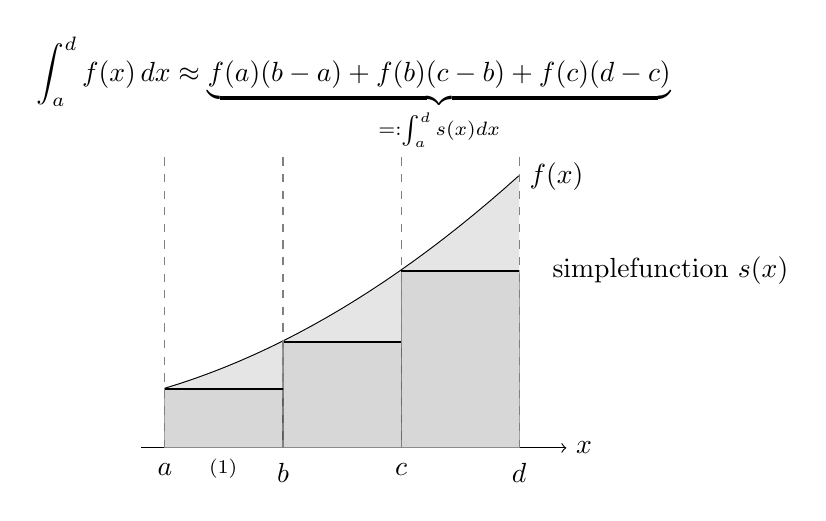
\begin{tikzpicture}[scale=1.5]
  % Axes
  \draw[->] (-0.2,0) -- (3.4,0) node[right] {$x$};
 % \draw[->] (0,-0.1) -- (0,2.6) node[above] {$y$};
  % Continuous function f(x)
  \draw[thick,domain=0:3,smooth] plot(\x,{0.5+0.3*\x+0.1*\x*\x}) node[right] {$f(x)$};
  % Shade area under f(x)
  \fill[gray!20] (0,0) -- plot[domain=0:3] (\x,{0.5+0.3*\x+0.1*\x*\x}) -- (3,0) -- cycle;
  % Lower simple function: left-endpoint rectangles for [0,1], [1,2], [2,3]
  \draw[fill=gray!50,opacity=0.35] (0,0) rectangle (1,0.5);
  \node at (0.5,-0.2) {$\cluster^{(1)}$}; 
  \draw[fill=gray!50,opacity=0.35] (1,0) rectangle (2,0.9);
  \draw[fill=gray!50,opacity=0.35] (2,0) rectangle (3,1.5);
  % Step lines of the simple function
  \draw[thick] (0,0.5)--(1,0.5);
  \draw[thick] (1,0.9)--(2,0.9);
  \draw[thick] (2,1.5)--(3,1.5);
  \node[above left] at (0.8,0.5) {};
  % Dashed partition lines
  \foreach \x in {0,1,2,3} \draw[dashed,gray] (\x,0) -- (\x,2.5);
  % Labels
  \node[anchor=north] at (0,-0.05) {$a$};
  \node[anchor=north] at (1,-0.05) {$b$};
  \node[anchor=north] at (2,-0.05) {$c$};
  \node[anchor=north] at (3,-0.05) {$d$};
  \node at (1.6,3.0) {$\displaystyle \int_a^d f(x)\,dx \approx \underbrace{f(a)(b-a) + f(b)(c-b)+f(c)(d-c)}_{=:\int_a^d s(x)dx}$};
  \node [anchor=west] at (3.2,1.5) {\gls{simplefunction} $s(x)$};
\end{tikzpicture}
\end{figure}
 It is useful to think of the Lebesgue integral as a \gls{function} that maps 
 an integrable \gls{function} $f$ to the value of its integral, 
	$$ f \mapsto \int_{\featurevec} f(\featurevec) d\featurevec.$$ 
	The precise defintion of this \gls{function}, including its \gls{domain} 
	which are the integrable \glspl{function}, is a corner-stone of 
	measure theory \cite[Ch. 1]{RudinBook}.
					\\ 
		See also: \gls{function}.},
	first={Lebesgue integral},
	type=math, 
	firstplural={Lebesgue integral}
}

\newglossaryentry{cdf}
{name={cumulative distribution function (cdf)},
	description={The \index{cumulative distribution function (cdf)} cdf 
	$\cdf{\feature}{\eta}$ of a real-valued \gls{rv} $\feature$ is \cite{AshProbMeasure,papoulis}
	$$\cdf{\feature}{\eta} \defeq \prob{\feature \leq \eta}.$$
					\\ 
		See also: \gls{pdf}, \gls{probdist}, \gls{rv}.},
	first={cumulative distribution function (cdf)},
	firstplural={cumulative distribution functions (cdfs)}, 
	plural={cdfs}, 
	type=math,
	text={cdf} 
}

\newglossaryentry{weightedgraph}
{name={weighted graph},
	description={A \gls{graph}\index{weghted graph} whose edges 
	are assigned numeric weights. Typically, these edge weights 
	are non-negative real numbers. For example, if a graph represents 
	a road network with nodes being intersections and edges representing 
	road segments, the edge weight could represent the capacity (measured 
	in maximum vehicles per hour) of the road segment \cite{NewmannBook}.  
					\\ 
		See also: \gls{graph}.},
	first={weighted graph},
	type=math,
	firstplural={weighted graphs}, 
	plural={weighted graphs}, 
	text={weighted graph} 
}



\newglossaryentry{graph}
{name={graph},
 description={A graph\index{graph} $\graph = \pair{\nodes}{\edges}$ 
 is a pair that consists of a node set $\nodes$ and an edge set $\edges$. 
 In its most general form, a graph is specified by a \gls{map} that 
 assigns each edge $\edgeidx \in \edges$ a pair of nodes \cite{RockNetworks}. 
 Unless specified otherwise, the term graph refers to an undirected graph. 
 A simple undirected graph is obtained by identifying each edge $\edgeidx \in \edges$ 
 with a set that contains two different nodes $\{\nodeidx,\nodeidx'\}$. 
 Weighted graphs also specify numeric \gls{weights} $\edgeweight_{\edgeidx}$ for each 
 edge $\edgeidx \in \edges$.
					\\ 
		See also: \gls{map}, \gls{weights}.},
 first={graph},
 text={graph}, 
 type=math
}

\newglossaryentry{uncertainty}
{name={uncertainty},
	description={In the context of \gls{ml}, uncertainty\index{uncertainty} refers to the presence of multiple 
		plausible outcomes or \glspl{explanation} based on available \gls{data}. For example, the 
		\gls{prediction} $\hat{\hypothesis}(\featurevec)$ produced by a trained \gls{ml} \gls{model} $\hat{\hypothesis}$
	 	often reflects a range of possible values for the true \gls{label} of a given \gls{datapoint}. 
	 	The broader this range, the greater the associated uncertainty. \Gls{probability} theory 
	 	allows us to represent, quantify, and reason about uncertainty in a 
	 	mathematically rigorous manner.
					\\ 
		See also: \gls{probmodel}, \gls{risk}, \gls{entropy}, \gls{variance}. },
	first={uncertainty},
	text={uncertainty}
}

\newglossaryentry{ucb}
{name={upper confidence bound (UCB)},
	description={Consider\index{upper confidence bound (UCB)} an \gls{ml} 
		application that requires selecting, at each time step $\iteridx$, an action $\arm_{\iteridx}$ 
		from a finite set of alternatives $\actionset$. The utility of selecting action $\arm_{\iteridx}$ 
		is quantified by a numeric \gls{reward} signal $\reward^{(\arm_{\iteridx})}$. 
		A widely used \gls{probmodel} for this type of sequential decision-making problem 
		is the \gls{stochastic} \gls{mab} setting \cite{Bubeck2012}. In this \gls{model}, 
		the \gls{reward} $\reward^{(\arm)}$ is viewed as the \gls{realization} of a \gls{rv} 
		with unknown \gls{mean} $\mu^{(\arm)}$. Ideally, we would always choose the 
		action with the largest expected \gls{reward} $\mu^{(\arm)}$, but these 
		\glspl{mean} are unknown and must be estimated from observed \gls{data}. Simply 
		choosing the action with the largest estimate $\widehat{\mu}^{(\arm)}$ can 
		lead to suboptimal outcomes due to estimation \gls{uncertainty}. The UCB strategy 
		addresses this by selecting actions not only based on their estimated \glspl{mean} but 
		also by incorporating a term that reflects the \gls{uncertainty} in these estimates—favoring 
		actions with a high-potential \gls{reward} and high \gls{uncertainty}. Theoretical guarantees 
		for the performance of UCB strategies, including logarithmic \gls{regret} bounds, are established in \cite{Bubeck2012}.
					\\ 
		See also: \gls{optimism in the face of uncertainty}, \gls{reward}, \gls{mab}, \gls{uncertainty}, \gls{regret}.},
	first={upper confidence bound (UCB)},
	text={UCB} 
}

\newglossaryentry{mab}
{name={multiarmed bandit (MAB)},
	description={An MAB \index{multiarmed bandit (MAB)} problem is a precise 
	formulation of a sequential decision-making task under \gls{uncertainty}. At each 
	discrete time step $\iteridx$, a learner selects one of several possible 
	actions—called arms—from a finite set $\actionset$. Pulling arm $\arm$ at time 
	$\iteridx$ yields a \gls{reward} $\reward^{(\arm,\iteridx)}$ that is drawn from an unknown 
	\gls{probdist} $\prob{\reward^{(\arm,\iteridx)}}$. We obtain different classes 
	of MAB problems by placing different restrictions on this \gls{probdist}. In the simplest 
	setting, the \gls{probdist} $\prob{\reward^{(\arm,\iteridx)}}$ does not depend on $\timeidx$. 
		Given an MAB problem, the goal is to construct \gls{ml} methods that maximize the cumulative 
		\gls{reward} over time by strategically balancing exploration (i.e., gathering information 
		about uncertain arms) and exploitation (i.e., selecting arms known to perform well). 
		MAB problems form an important special case of \gls{reinforcementlearning} problems \cite{Bubeck2012}, \cite{SuttonEd2}.
					\\ 
		See also: \gls{reward}, \gls{regret}.},
	first={MAB},
	text={MAB}
}



\newglossaryentry{optimism in the face of uncertainty}
{name={optimism in the face of uncertainty},
	description={\gls{ml}\index{optimism in the face of uncertainty} methods learn \glspl{modelparam} $\weights$ 
		according to some performance criterion $\bar{f}(\weights)$. However, they usually 
		cannot access $\bar{f}(\weights)$ directly but rely on an estimate (or approximation) 
		$f(\weights)$ of $\bar{f}(\weights)$. As a case in point, \gls{erm}-based methods use 
		the average \gls{loss} on a given \gls{dataset} (i.e., the \gls{trainset}) as an estimate 
		for the \gls{risk} of a \gls{hypothesis}. Using a \gls{probmodel}, one can construct 
		a confidence interval $\big[ l^{(\weights)},  u^{(\weights)} \big]$ for each choice $\weights$ for the \glspl{modelparam}.
		One simple construction is $l^{(\weights)} \defeq f(\weights) - \sigma/2$, $u^{(\weights)} \defeq f(\weights)+ \sigma/2$, 
	    	with $\sigma$ being a measure of the (expected) deviation of $f(\weights)$ from $\bar{f}(\weights)$.
		We can also use other constructions for this interval as long as they ensure that $\bar{f}(\weights) \in\big[ l^{(\weights)},  u^{(\weights)} \big]$ 
		with a sufficiently high \gls{probability}. An optimist chooses the \glspl{modelparam} 
		according to the most favorable—yet still plausible—value $\tilde{f}(\weights) \defeq  l^{(\weights)}$ 
		of the performance criterion (see Fig. \ref{fig_optimism_dict}). Two examples of \gls{ml} methods that use such an optimistic 
		construction of an \gls{objfunc} are \gls{srm} \cite[Ch. 11]{ShalevMLBook} and \gls{ucb} methods 
		for sequential decision making \cite[Sec. 2.2]{Bubeck2012}. 
		\begin{figure}[H]
			\begin{center}
			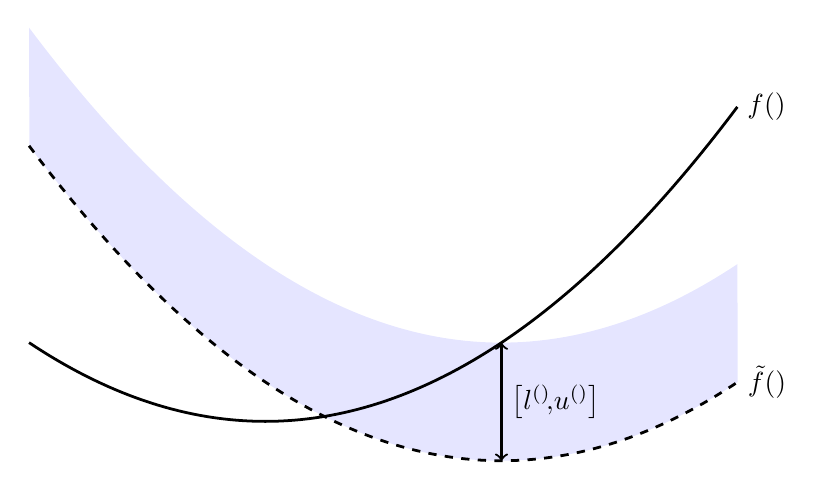
\begin{tikzpicture}[x=3cm, y=1cm]
  			% Filled band around the quadratic curve with different boundary curves
			\fill[blue!10] 
			(-1, 5) -- plot[domain=-2:1, samples=100] ({\x+1}, {\x*\x + 1}) -- 
			plot[domain=1:-2, samples=100] ({\x+1}, {\x*\x - 0.5}) -- cycle;
  			\node[anchor=west] at (2, 4) {$f(\weights)$};
  			\draw[line width=1, domain=-2:1, samples=100,dashed] plot  ({\x+1}, {\x*\x -0.5}) node[right] {$\tilde{f}(\weights)$};
   			\draw[line width=1, domain=-1:2, samples=100] plot ({\x}, {\x*\x});
  			\draw[<->, thick] (1, -0.5) -- (1, 1) node[midway, right] {$\big[ l^{(\weights)}\!,\!u^{(\weights)} \big]$};
			\end{tikzpicture}
			\caption{\gls{ml} methods learn \glspl{modelparam} $\weights$ by using some estimate of $f(\weights)$ for 
			the ultimate performance criterion $\bar{f}(\weights)$. Using a \gls{probmodel}, one can use $f(\weights)$ to 
			construct confidence intervals $\big[ l^{(\weights)},  u^{(\weights)} \big]$, which contain $\bar{f}(\weights)$  
			with a high probability. The best plausible performance measure for a specific choice $\weights$ of \glspl{modelparam} 
			is $\tilde{f}(\weights) \defeq l^{(\weights)}$. \label{fig_optimism_dict}} 
			\end{center}
		\end{figure}
		See also: \gls{objfunc}, \gls{optmethod}, \gls{gdmethod}, \gls{ucb}.},
	first={optimism in the face of uncertainty},
	text={optimism in the face of uncertainty} 
}

\newglossaryentry{empgraph}
{name={federated learning network (FL network)},
	description={An \gls{fl} network\index{federated learning network (FL network)} consists of 
		an undirected weighted \gls{graph} $\graph$. The nodes of $\graph$ represent \glspl{device} 
		that can access a \gls{localdataset} and train a \gls{localmodel}. The edges of $\graph$ represent 
		communication links between \glspl{device} as well as statistical similarities between their \glspl{localdataset}. 
		A principled approach to train the \glspl{localmodel} is \gls{gtvmin}. The solutions of \gls{gtvmin} are local 
		\glspl{modelparam} that optimally balance the \gls{loss} incurred on \glspl{localdataset} with their \gls{discrepancy} 
		across the edges of $\graph$.
	    			\\ 
		See also: \gls{fl}, \gls{graph}, \gls{device}, \gls{gtvmin}.},
	first={federated learning network (FL network)},
	text={FL network} 
}

\newglossaryentry{norm}
{name={norm},
	description={A norm\index{norm} is a \gls{function} that maps each (\gls{vector}) element 
		of a \gls{vectorspace} to a nonnegative real number. This \gls{function} must be 
		homogeneous and definite, and it must satisfy the triangle inequality \cite{HornMatAnalysis}.
		\\
		See also: \gls{function}, \gls{vector}, \gls{vectorspace}.},
	first={norm},
	text={norm} 
}

\newglossaryentry{dualnorm}
{name={dual norm},
	description={Every \gls{norm} $\normgeneric{\cdot}{}$ defined on a \gls{euclidspace} $\mathbb{R}^{\dimlocalmodel}$ 
		has an associated dual \gls{norm}, which is denoted by $\normgeneric{\cdot}{*}$ and defined as 
		$\normgeneric{\vy}{*} \defeq \sup_{\norm{\vx}{} \le 1} \vy\,^{T} \vx$. 
		The dual \gls{norm} measures the largest possible inner product between $\vy$ 
		and any \gls{vector} in the unit ball of the original \gls{norm}. For further details, see 
		\cite[Sec.~A.1.6]{BoydConvexBook}.
					\\ 
		See also: \gls{norm}, \gls{euclidspace}, \gls{vector}.},
	first={dual norm},
	text={dual norm}
}

\newglossaryentry{geometricmedian}
{name={geometric median (GM)},
	description={The GM\index{geometric median (GM)} of a set of input \glspl{vector} $\vx^{(1)}, \,\ldots, \,\vx^{(\samplesize)}$ 
		in $\mathbb{R}^{\dimlocalmodel}$ is a point $\vz \in \mathbb{R}^{\dimlocalmodel}$ that 
		minimizes the sum of distances to the \glspl{vector} \cite{BoydConvexBook} such that 
		\begin{equation} 
			\label{equ_geometric_median_dict}
		\vz \in \argmin_{\vy \in \mathbb{R}^{\dimlocalmodel}} \sum_{\sampleidx=1}^{\samplesize} \normgeneric{\vy - \vx^{(\sampleidx)}}{2}.
		\end{equation} 
		Fig. \ref{opt_cond_GM_dict} illustrates a fundamental property of the GM:
		If $\vz$ does not coincide with any of the input \glspl{vector}, then the unit \glspl{vector} pointing 
		from $\vz$ to each $\vx^{(\sampleidx)}$ must sum to zero—this is the zero-\gls{subgradient}  
		(optimality) condition for \eqref{equ_geometric_median_dict}. It turns out that the solution to 
		\eqref{equ_geometric_median_dict} cannot be arbitrarily pulled away from trustworthy input 
		\glspl{vector} as long as they are the majority \cite[Th. 2.2]{Lopuhaae1991}.
	  	\begin{figure}[H]
  		\begin{center}
			\begin{tikzpicture}[scale=2, thick, >=stealth]
%				% Central model w
				\coordinate (w) at (3,0);
				\fill (w) circle (1.2pt) node[below right] {$\vz$};
% Clean nodes
				\coordinate (w2) at (0.5,0.3);
				\coordinate (w3) at (0.7,0.7);
				\fill (w2) circle (1pt) node[above left] {$\vx^{(1)}$};
				\fill (w3) circle (1pt) node[above left] {$\vx^{(2)}$};
			    \node[anchor=west] at ($(w2) +(-0.2,0.9)$) {\textbf{clean}};
%				% Dashed lines from w to good nodes
				\draw[dashed] (w) -- (w2);
				\draw[dashed] (w) -- (w3);
%				% Draw unit vectors (scaled to 1cm)
				\draw[->, thick, red] (w) -- ($(w)!1cm!(w2)$) ;
				\draw[->, thick, red] (w) -- ($(w)!1cm!(w3)$) node[pos=0.9, right,yshift=7pt] {$\frac{\vx^{(2)}- \vz}{\normgeneric{\vx^{(2)}-\vz}{2}}$};
%				\node at (-0.2,1.4) {\textbf{Clean}};
				\coordinate (w4) at (5,0.2);
				\node at (5,0.6) {\textbf{perturbed}};
				\fill (w4) circle (1pt) node[below left] {$\vx^{(3)}$};
				\draw[->, thick, red] (w) -- ($(w)!1cm!(w4)$) ;
%		% Optional dotted line from w to bad
		\end{tikzpicture}
		\caption{\label{opt_cond_GM_dict}
			Consider a solution $\vz$ of \eqref{equ_geometric_median_dict} that does not coincide 
			with any of the input \glspl{vector}. The optimality condition for \eqref{equ_geometric_median_dict} 
			requires that the unit \glspl{vector} from $\vz$ to the input \glspl{vector} sum to zero.}
			\end{center}
		\end{figure}
		See also: \gls{vector}, \gls{subgradient}.},
	first={geometric median},
	text={GM}
}


\newglossaryentry{explanation}
{name={explanation}, plural={explanations},
	description={One approach to enhance the \gls{transparency} of an \gls{ml} method for its human user 
		is to provide an explanation\index{explanation} alongside the \glspl{prediction} delivered 
		by the method. Explanations can take different forms. For instance, they may 
        		consist of human-readable text or quantitative indicators, such as \gls{feature} 
        		importance scores for the individual \glspl{feature} of a given \gls{datapoint}~\cite{Molnar2019}. 
	   	Alternatively, explanations can be visual—for example, intensity \glspl{map} that highlight 
	   	image regions that drive the \gls{prediction} \cite{GradCamPaper}. 
       		Fig.\ \ref{fig_explanation_dict} illustrates two types of explanations. The first 
       		is a local linear approximation $g(\featurevec)$ of a nonlinear trained \gls{model} 
       		$\learnthypothesis(\featurevec)$ around a specific \gls{featurevec} $\featurevec'$, 
       		as used in the method \gls{lime}. 
        		The second form of explanation depicted in the figure is a sparse set of \glspl{prediction} 
       		$\learnthypothesis(\featurevec^{(1)}), \learnthypothesis(\featurevec^{(2)}), \learnthypothesis(\featurevec^{(3)})$ 
       		at selected \glspl{featurevec}, offering concrete reference points for the user. 
	 	\begin{figure}[H]
	   		\begin{center}
	 		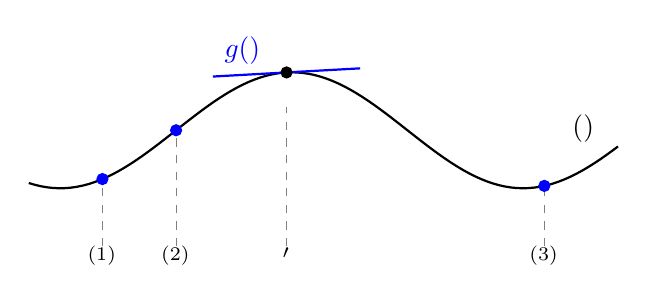
\begin{tikzpicture}[x=0.5cm]
	 		\begin{axis}[
	 			hide axis,
	 			xmin=-3, xmax=6,
	 			ymin=0, ymax=6,
	 			domain=0:6,
	 			samples=100,
	 			width=10cm,
	 			height=6cm,
	 			clip=false
	 		   ]
	 		% Original nonlinear function h(x)
			\addplot[thick, domain=-2:6] {2 + sin(deg(x))} 
	   		     node[pos=0.9, above right, yshift=10pt] {$\learnthypothesis(\featurevec)$};
	 		% Tangent line as local linear approximation at x = 1.5
	 		% h(3) = 2 + sin(3), h'(3) = cos(3)
	 		\addplot[blue, thick, domain=0.5:2.5] 
	 		{2 + sin(deg(1.5)) + cos(deg(1.5))*(x - 1.5)}
	 		node[pos=0.2, above] {$g(\featurevec)$};
	 		% Mark point of approximation
	 		\addplot[mark=*] coordinates {(1.5, {2 + sin(deg(1.5))})};
	 		    % Vertical dashed line (ruler) at x = 1.5
			\addplot[dashed, gray] coordinates {(1.5,0) (1.5,2.4)};
	 		\node at (axis cs:1.5, -0.2) {$\featurevec'$};
	      		% add function values for finite set of featurevecs
	       		\addplot[mark=*,blue] coordinates {(-1, {2 + sin(deg(-1))})};
	       		\addplot[dashed, gray] coordinates {(-1,0) (-1,{2 + sin(deg(-1))})};
	       		\node at (axis cs:-1, -0.2) {$\featurevec^{(1)}$};
	 	   	\addplot[mark=*,blue] coordinates {(0, {2 + sin(deg(0))})};
	 	   	\addplot[dashed, gray] coordinates {(0,0) (0,{2 + sin(deg(0))})};
	 	   	\node at (axis cs:0, -0.2) {$\featurevec^{(2)}$};
	 	   	\addplot[mark=*,blue] coordinates {(5, {2 + sin(deg(5))})};
	 	   	\addplot[dashed, gray] coordinates {(5,0) (5,{2 + sin(deg(5))})};
	 	   	\node at (axis cs:5, -0.2) {$\featurevec^{(3)}$};
	% 		    % Plot the two points
	% 		    % Coordinates of the two points
	% 		\pgfmathsetmacro{\xA}{-1.5}
	% 		\pgfmathsetmacro{\xB}{3}
	% 		\pgfmathsetmacro{\yA}{2 + sin(deg(\xA))}
	% 		\pgfmathsetmacro{\yB}{2 + sin(deg(\xB))}
	 		\end{axis}
	% 	\vspace*{-10mm}
		\end{tikzpicture}
	 	\end{center}
	 	\caption{A trained \gls{model} $\learnthypothesis(\featurevec)$ can be explained 
	     	locally at some point $\featurevec'$ by a linear approximation $g(\featurevec)$. 
	     	For a \gls{differentiable} $\learnthypothesis(\featurevec)$, this approximation is 
	     	determined by the \gls{gradient} $\nabla \learnthypothesis(\featurevec')$. Another 
	     	form of explanation could be the \gls{function} values $\learnthypothesis\big(\featurevec^{(\sampleidx)} \big)$ 
	     	for $\sampleidx=1, 2, 3$. 
		\label{fig_explanation_dict}}
	 	\end{figure} 
		See also: \gls{ml}, \gls{prediction}, \gls{feature}, \gls{datapoint}, \gls{classification}.},
	first={explanation},
	text={explanation} 
}

\newglossaryentry{risk}
{name={risk},
	description={Consider\index{risk} a \gls{hypothesis} $\hypothesis$ used to predict the \gls{label} 
		$\truelabel$ of a \gls{datapoint} based on its \glspl{feature} $\featurevec$. We measure 
		the quality of a particular \gls{prediction} using a \gls{lossfunc} $\lossfunc{(\featurevec,\truelabel)}{\hypothesis}$. 
		If we interpret \glspl{datapoint} as the \glspl{realization} of \gls{iid} \glspl{rv}, 
		the $\lossfunc{(\featurevec,\truelabel)}{\hypothesis}$ also becomes the \gls{realization} 
		of a \gls{rv}. The \gls{iidasspt} allows us to define the risk of a \gls{hypothesis} 
		as the expected \gls{loss} $\expect \big\{\lossfunc{(\featurevec,\truelabel)}{\hypothesis} \big\}$. 
		Note that the risk of $\hypothesis$ depends on both the specific choice for the \gls{lossfunc} and the 
		\gls{probdist} of the \glspl{datapoint}.
					\\ 
		See also: \gls{iid} \gls{rv}, \gls{iidasspt}, \gls{loss}, \gls{probdist}.},
	first={risk},
	text={risk} 
}

\newglossaryentry{actfun}
{name={activation function},
	description={Each\index{activation function} artificial neuron within an \gls{ann} is 
		assigned an \gls{activation} \gls{function} $\actfun(\cdot)$ that maps a weighted 
		combination of the neuron inputs $\feature_{1}, \,\ldots, \,\feature_{\nrfeatures}$ 
		to a single output value $a = \actfun\big(\weight_{1} \feature_{1}+\ldots+\weight_{\nrfeatures} \feature_{\nrfeatures} \big)$. 
		Note that each neuron is parameterized by the \gls{weights} $\weight_{1}, \,\ldots, \,\weight_{\nrfeatures}$.
					\\ 
		See also: \gls{ann}, \gls{activation}, \gls{relu}.},
	first={activation function},
	text={activation function} 
}

\newglossaryentry{distributedalgorithm}
{name={distributed algorithm},
	description={A\index{distributed algorithm} distributed \gls{algorithm} is an \gls{algorithm} designed for 
		a special type of computer, i.e., a collection of interconnected computing devices (or nodes). 
		These devices communicate and coordinate their local computations by exchanging 
		messages over a network \cite{IntroDistAlg}, \cite{ParallelDistrBook}. Unlike a classical \gls{algorithm}, 
		which is implemented on a single \gls{device}, a distributed \gls{algorithm} is 
		executed concurrently on multiple \glspl{device} with computational capabilities. 
		Similar to a classical \gls{algorithm}, a distributed \gls{algorithm} can be modeled as a 
		set of potential executions. However, each execution in the distributed setting involves 
		both local computations and message-passing \glspl{event}. A generic execution might look as 
		follows:
		\[
		\begin{array}{l}
			\text{Node 1: } {\rm input}_1, \,s_1^{(1)}, \,s_2^{(1)}, \,\ldots, \,s_{T_1}^{(1)}, \,{\rm output}_1; \\
			\text{Node 2: } {\rm input}_2, \,s_1^{(2)}, \,s_2^{(2)}, \,\ldots, \,s_{T_2}^{(2)}, \,{\rm output}_2; \\
			\quad \vdots \\
			\text{Node N: } {\rm input}_N, \,s_1^{(N)}, \,s_2^{(N)}, \,\ldots, \,s_{T_N}^{(N)}, \,{\rm output}_N.
		\end{array}
		\]
		Each \gls{device} $\nodeidx$ starts from its own local input and performs a sequence of 
		intermediate computations $s_{\iteridx}^{(\nodeidx)}$ at discrete-time instants $\iteridx = 1, \,\dots, \,T_\nodeidx$. 
		These computations may depend on both the previous local computations at the \gls{device} 
		and the messages received from other \glspl{device}. One important application of distributed 
		\glspl{algorithm} is in \gls{fl} where a network of \glspl{device} collaboratively trains a personal \gls{model} 
		for each \gls{device}. 
					\\ 
		See also: \gls{algorithm}, \gls{device}, \gls{event}, \gls{fl}, \gls{model}.
		},
	first={distributed algorithm}, 
	text={distributed algorithm}
}


\newglossaryentry{algorithm}
{name={algorithm}, plural={algorithms},
 	description={An\index{algorithm} algorithm is a precise, step-by-step specification for 
  		producing an output from a given input within a finite number of well-defined 
		computational steps \cite{Cormen:2022aa}. For example, an \gls{gdmethod} for \gls{linreg} 
		is an algorithm that explicitly describes how to map a given \gls{trainset} 
		into \glspl{modelparam} through a sequence of \glspl{gradstep}. The precise form of 
		an algorithm depends on the available computational infrastructure. For example, if 
		this infrastructure allows to compute a \gls{inverse} \gls{matrix}, then we can 
		define a \gls{linreg} algorithm using the \gls{normalequations}. In contrast, if 
		the computational infrastructe does only allow for basic arithmetic (mulilication and addition), 
		the \gls{normalequations} need to be somehow translated into a sequence of arithmetic 
		operations (e.g., as in \glspl{gdmethod}). 
		To study algorithms rigorously, we can represent (or approximate) them by different 
			mathematical structures \cite{Sipser2013}. One approach is to represent an algorithm 
			as a collection of possible executions. Each individual execution is then a 
			sequence of the form $${\rm input}, \,s_1, \,s_2, \,\ldots, \,s_T, \,{\rm output}.$$ 
			This sequence starts from an input and progresses via intermediate steps until an 
			output is delivered. Crucially, an algorithm encompasses more than just a mapping 
			from input to output; it also includes intermediate computational 
     		steps $s_1, \,\ldots, \,s_T$.
				\\ 
		See also: \gls{linmodel}, \gls{trainset}, \glspl{modelparam}, \gls{gradstep}, \gls{model}, \gls{stochastic}.},
	first={algorithm},
	text={algorithm} 
}

\newglossaryentry{stochalgorithm}
{name={stochastic algorithm}, 
 plural={stochastic algorithms},
	description={A\index{stochastic algorithm} \gls{stochastic} \gls{algorithm} uses a random mechanism 
		during its execution. For example, \gls{stochGD} uses a randomly selected subset of \glspl{datapoint} 
		to compute an approximation for the \gls{gradient} of an \gls{objfunc}. We can represent a 
		\gls{stochastic} \gls{algorithm} by a \glspl{stochproc}, i.e., the possible execution sequence is the possible outcomes of 
		a \gls{randomexperiment} \cite{BertsekasProb}, \cite{RandomizedAlgos}, \cite{Gallager13}.		
		\\ 
		See also: \gls{stochastic}, \gls{algorithm}, \gls{stochGD}, \gls{datapoint}, \gls{gradient}, \gls{objfunc}, \gls{stochproc}, 
		\gls{randomexperiment}, \gls{optmethod}, \gls{gdmethod}. },
	first={stochastic algorithm},
	text={stochastic algorithm} 
}

\newglossaryentry{batchlearning}
{name={batch learning},
	description={In \gls{batch} learning\index{batch learning} (also known as offline learning), the \gls{ml} \gls{model} 
		is trained on the entire \gls{dataset} in a single training iteration, instead of updating it incrementally as \gls{data} arrive. 
		All available \gls{data} are inputted into a learning \gls{algorithm}, resulting in a \gls{model} that can make \glspl{prediction}. 
		Since these \glspl{dataset} tend to be large, training is computationally expensive and time-consuming, 
		so it is typically performed offline. After learning, the \gls{model} will be static and will not adapt to new \gls{data} automatically. 
		Updating the \gls{model} with new information requires retraining the \gls{model} entirely. Once the \gls{model} has been trained, 
		it is launched into production where it cannot be updated. Training a \gls{model} can take many hours, so many \glspl{model} in production 
		settings are updated cyclically on a periodic schedule when the \gls{data} distribution is stable. For example, a retail analytics team 
		could retrain their demand forecast \gls{model} every Sunday using the previous week's sales \gls{data} to predict next week's demand. 
		If a system needs to be constantly updated to rapidly changing \gls{data}, such as in stock price \gls{prediction}, a more adaptable solution 
		such as \gls{onlinelearning} is necessary.
		\\
		See also: \gls{batch}, \gls{model}, \gls{dataset}, \gls{onlinelearning}. },
	first={batch learning}, 
	text={batch learning}
}

\newglossaryentry{onlinelearning}
{name={online learning},
	description={Some \gls{ml} methods \index{online learning} are designed to process \gls{data} in a sequential 
		manner, updating their \glspl{modelparam} one at a time, as new \glspl{datapoint} become available. 
		A typical example is time-series \gls{data}, such as daily \gls{minimum} and \gls{maximum} temperatures 
		recorded by an \gls{fmi} weather station. These values form a chronological sequence 
		of observations. During each time step $\timeidx$, online learning methods update (or refine)  
		the current \gls{hypothesis} $\hypothesis^{(\timeidx)}$ (or \glspl{modelparam} $\weights^{(\timeidx)}$) 
		based on the newly observed \gls{datapoint} $\datapoint^{(\timeidx)}$. 
		\\ 
		See also: \gls{onlineGD}, \gls{onlinealgorithm}. },
	first={online learning},
	text={online learning} 
}

\newglossaryentry{onlinealgorithm}
{name={online algorithm},
	description={An\index{online algorithm} online \gls{algorithm} processes input \gls{data} incrementally, 
		receiving \glspl{datapoint} sequentially and making decisions or producing outputs (or decisions) immediately 
		without having access to the entire input in advance \cite{PredictionLearningGames}, \cite{HazanOCO}. 
		Unlike an offline \gls{algorithm}, which has the entire input available from the start, an online \gls{algorithm} 
		must handle \gls{uncertainty} about future inputs and cannot revise past decisions. Similar to an 
		offline \gls{algorithm}, we represent an online \gls{algorithm} formally as a collection of possible 
		executions. However, the execution sequence for an online \gls{algorithm} has a distinct structure as follows:
		$${\rm in}_{1}, \,s_1, \,{\rm out}_{1}, \,{\rm in}_{2}, \,s_2, \,{\rm out}_{2}, \,\ldots, \,{\rm in}_{T}, \,s_T, \,{\rm out}_{T}.$$ 
		Each execution begins from an initial state (i.e., \(\text{in}_{1}\)) and proceeds through alternating 
		computational steps, outputs (or decisions), and inputs. Specifically, at step \(\iteridx\), 
		the \gls{algorithm} performs a computational step \(s_{\iteridx}\), generates an output \(\text{out}_{\iteridx}\), 
		and then subsequently receives the next input (\gls{datapoint}) \(\text{in}_{\iteridx+1}\). A 
		notable example of an online \gls{algorithm} in \gls{ml} is \gls{onlineGD}, which incrementally 
		updates \glspl{modelparam} as new \glspl{datapoint} arrive. 
					\\ 
		See also: \gls{algorithm}, \gls{data}, \gls{datapoint}, \gls{uncertainty}, \gls{ml}, \gls{onlineGD}, \glspl{modelparam}, \gls{onlinelearning}.},
	first={online algorithm},
	text={online algorithm} 
}


\newglossaryentry{transparency}
{name={transparency},
	description={Transparency\index{transparency} is a fundamental requirement for 
		\gls{trustAI} \cite{HLEGTrustworhtyAI}. In the context of \gls{ml} 
		methods, transparency is often used interchangeably with \gls{explainability} 
		\cite{JunXML2020}, \cite{gallese2023ai}. However, in the broader scope of \gls{ai} 
		systems, transparency extends beyond \gls{explainability} and includes providing information 
		about the system’s limitations, reliability, and intended use. 
		In medical diagnosis systems, transparency requires disclosing the confidence level 
		for the \glspl{prediction} delivered by a trained \gls{model}. In credit scoring, 
		\gls{ai}-based lending decisions should be accompanied by explanations of 
		contributing factors, such as income level or credit history. These explanations 
		allow humans (e.g., a loan applicant) to understand and contest automated decisions. 
		Some \gls{ml} methods inherently offer transparency. For example, \gls{logreg} 
		provides a quantitative measure of \gls{classification} reliability through the value $|\hypothesis(\featurevec)|$. 
		\Glspl{decisiontree} are another example, as they allow human-readable decision rules \cite{rudin2019stop}.
		Transparency also requires a clear indication when a user is engaging with an \gls{ai} system. 
		For example, \gls{ai}-powered chatbots should notify users that they are interacting with an 
		automated system rather than a human. Furthermore, transparency encompasses comprehensive 
		documentation detailing the purpose and design choices underlying the \gls{ai} system. 
		For instance, \gls{model} datasheets \cite{DatasheetData2021} and \gls{ai} system cards \cite{10.1145/3287560.3287596} 
		help practitioners understand the intended use cases and limitations of an \gls{ai} system \cite{Shahriari2017}.
					\\ 
		See also: \gls{trustAI}, \gls{explainability}.},
	first={transparency}, 
	text={transparency} 
}



\newglossaryentry{sensattr}
{name={sensitive attribute}, plural={sensitive attributes},
	description={\gls{ml}\index{sensitive attribute} revolves around learning a \gls{hypothesis} \gls{map} that allows 
		us to predict the \gls{label} of a \gls{datapoint} from its \glspl{feature}. In some 
		applications, we must ensure that the output delivered by an \gls{ml} system does 
		not allow us to infer sensitive attributes of a \gls{datapoint}. Which part 
		of a \gls{datapoint} is considered a sensitive attribute is a design 
		choice that varies across different application domains.
					\\ 
		See also: \gls{ml}, \gls{hypothesis}, \gls{map}, \gls{label}, \gls{datapoint}, \gls{feature}.},
	first={sensitive attribute},
	text={sensitive attribute} 
}


\newglossaryentry{sbm}
{name={stochastic block model (SBM)},
	description={The\index{stochastic block model (SBM)} SBM is a 
		probabilistic generative \gls{model} for an undirected \gls{graph} $\graph = \big( \nodes, \edges \big)$ 
		with a given set of nodes $\nodes$ \cite{AbbeSBM2018}. In its most basic variant, 
		the SBM generates a \gls{graph} by first randomly assigning each node $\nodeidx \in \nodes$ to 
		a \gls{cluster} index $\clusteridx_{\nodeidx} \in \{1, \,\ldots, \,\nrcluster\}$. A pair of different nodes in the 
		\gls{graph} is connected by an edge with \gls{probability} $p_{\nodeidx,\nodeidx'}$ that depends 
		solely on the \glspl{label} $\clusteridx_{\nodeidx}, \clusteridx_{\nodeidx'}$. 
		The presence of edges between different pairs of 
		nodes is statistically independent.
					\\ 
		See also: \gls{model}, \gls{graph}, \gls{cluster}, \gls{probability}, \gls{label}. },
	first={stochastic block model (SBM)},
	text={SBM} 
}

\newglossaryentry{deepnet}
{name={deep net}, plural={deep nets},
	description={A\index{deep net} deep net is an \gls{ann} with a (relatively) large number of 
		hidden \glspl{layer}. Deep learning is an umbrella term for \gls{ml} methods that use a deep 
		net as their \gls{model} \cite{Goodfellow-et-al-2016}.
				\\ 
		See also: \gls{ann}, \gls{layer}, \gls{ml}, \gls{model}.},
	first={deep net},
	text={deep net} 
}



\newglossaryentry{baseline}
{name={baseline},
    description={Consider\index{baseline} some \gls{ml} method that produces a learned 
    	\gls{hypothesis} (or trained \gls{model}) $\learnthypothesis \in \hypospace$. We evaluate the quality of a trained \gls{model} 
    	by computing the average \gls{loss} on a \gls{testset}. But how can we assess 
    	whether the resulting \gls{testset} performance is sufficiently good? How can we 
    	determine if the trained \gls{model} performs close to optimal such that there is little point 
   	in investing more resources (for \gls{data} collection or computation) to improve it? 
    	To this end, it is useful to have a reference (or baseline) level against which 
    	we can compare the performance of the trained \gls{model}. \\
	Such a reference value might be obtained from human performance, e.g., the misclassification rate of dermatologists 
    	who diagnose cancer from visual inspection of skin \cite{SkinHumanAI}. Another source for a baseline is an existing, 
    	but for some reason unsuitable, \gls{ml} method. For example, the existing \gls{ml} method 
    	might be computationally too expensive for the intended \gls{ml} application. 
    	Nevertheless, its \gls{testset} error can still serve as a baseline. Another, somewhat more principled, 
    	approach to constructing a baseline is via a \gls{probmodel}. In many cases, given a \gls{probmodel} $p(\featurevec,\truelabel)$,  
    	we can precisely determine the \gls{minimum} achievable \gls{risk} among any hypotheses
    	(not even required to belong to the \gls{hypospace} $\hypospace$) \cite{LC}. \\
    	This \gls{minimum} achievable \gls{risk} (referred to as the \gls{bayesrisk}) is the \gls{risk} 
    	of the \gls{bayesestimator} for the \gls{label} $\truelabel$ of a \gls{datapoint}, given
    	its \glspl{feature} $\featurevec$. Note that, for a given choice of \gls{lossfunc}, the 
    	\gls{bayesestimator} (if it exists) is completely determined by the \gls{probdist} 
		$\probdist$ \cite[Ch. 4]{LC}. However, computing the \gls{bayesestimator} 
		and \gls{bayesrisk} presents two main challenges. First, the \gls{probdist} 
		$\probdist$ is unknown and 
		must be estimated from observed \gls{data}. Second, even if $\probdist$ 
		were known, computing the \gls{bayesrisk} exactly may be computationally 
		infeasible \cite{cooper1990computational}. 
	A widely used \gls{probmodel} is the \gls{mvndist} $\pair{\featurevec}{\truelabel} \sim \mathcal{N}({\bm \mu},{\bm \Sigma})$ 
	for \glspl{datapoint} characterized by numeric \glspl{feature} and \glspl{label}.
	Here, for the \gls{sqerrloss}, the \gls{bayesestimator} is given by the posterior 
	\gls{mean} $\mu_{\truelabel|\featurevec}$ of the \gls{label} $\truelabel$, given the 
	\glspl{feature} $\featurevec$ \cite{LC}, \cite{GrayProbBook}. The corresponding \gls{bayesrisk} 
	is given by the posterior \gls{variance} 
	$\sigma^{2}_{\truelabel|\featurevec}$ (see Fig. \ref{fig_post_baseline_dict}).
	\begin{figure}[H]
		\begin{center}
		\begin{tikzpicture}
			% Axes
			\draw[->] (-1,0) -- (7,0) node[right] {$\truelabel$}; % x-axis
			% Gaussian distribution centered at 3 with variance 1
			\draw[thick,domain=-1:7,smooth,variable=\x] 
			  plot ({\x}, {2*exp(-0.5*((\x-3)^2))});
			% Dashed line indicating the mean of the Gaussian
			\draw[dashed] (3,0) -- (3,2.5);
			\node[anchor=south] at ([yshift=-5pt] 3,2.5) {\small $\mu_{\truelabel|\featurevec}$};
			% Double arrow indicating the variance
			\draw[<->,thick] (3-1,1) -- (3+1,1.0);
			\node[anchor=west] at ([yshift=2pt] 3,1.2) {\small $\sigma_{\truelabel|\featurevec}$};
			% Posterior variance label
			%\node[anchor=south east] at (3-0.5,1.8) {\small Posterior Variance};
			% x-axis marks with crosses
			  % x-axis marks with crosses
  			\foreach \x in {0.5} {
				\node[red] at (\x, 0) {\bf \large $\times$};
 			 }
  			% h(x) label for the first cross
  			\node[anchor=north] at (0.5,-0.2) {\small $\learnthypothesis(\featurevec)$};
		  \end{tikzpicture}
		\end{center}
		\caption{If the \glspl{feature} and the \gls{label} of a \gls{datapoint} are drawn 
		from a \gls{mvndist}, we can achieve the \gls{minimum} \gls{risk} (under \gls{sqerrloss}) 
		by using the \gls{bayesestimator} $\mu_{\truelabel|\featurevec}$ 
		to predict the \gls{label} $\truelabel$ of a \gls{datapoint} with \glspl{feature} $\featurevec$. The corresponding 
		\gls{minimum} \gls{risk} is given by the posterior \gls{variance} $\sigma^{2}_{\truelabel|\featurevec}$. We can use 
		this quantity as a baseline for the average \gls{loss} of a trained \gls{model} $\learnthypothesis$. \label{fig_post_baseline_dict}}
		\end{figure}
		See also: \gls{bayesrisk}, \gls{bayesestimator}.},
    first={baseline},
    text={baseline}
}

\newglossaryentry{kfoldcv}
{name={$k$-fold cross-validation ($k$-fold CV)},
 description={A method\index{$k$-fold cross-\gls{validation}} for evaluating the 
 \gls{gengap} of an \gls{erm}-based \gls{ml} method. The idea is to divide \gls{dataset} 
 $\dataset$ evenly into $k$ subsets (or folds) $\dataset^{(1)},\ldots,\dataset^{(k)}$
	\begin{figure}[htbp]
		\centering
	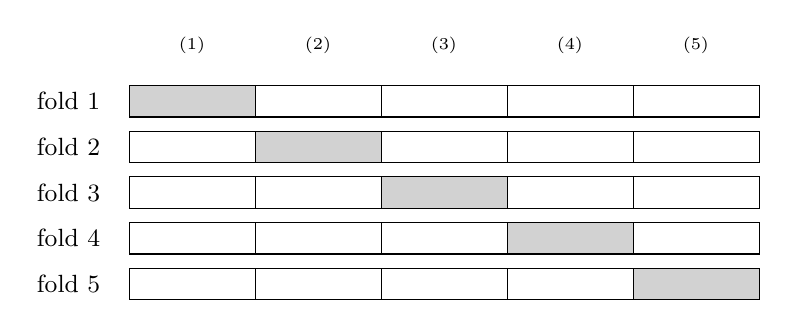
\begin{tikzpicture}[font=\small]
		\def\k{5}          % number of folds
		\def\cellw{1.6}    % width of one segment
		\def\cellh{0.40}   % height of one segment
		\def\gap{0.18}     % vertical gap between rows
		% rows: i = 1..k; columns: j = 1..k
		\foreach \i in {1,...,\k} {
			% row baseline y
			\pgfmathsetmacro{\y}{-(\i-1)*(\cellh+\gap)}
			% row label
			\node[anchor=east] at (-0.25,\y+0.5*\cellh) {fold \i};
			% draw k equal segments; shade the \i-th as validation
			\foreach \j in {1,...,\k} {
				\pgfmathsetmacro{\x}{(\j-1)*\cellw}
				\ifnum\i=\j
				\fill[gray!35] (\x,\y) rectangle ++(\cellw,\cellh);
				\draw (\x,\y) rectangle ++(\cellw,\cellh);
				\else
				\draw (\x,\y) rectangle ++(\cellw,\cellh);
				\fi
			}
		}
		% add labels D^{(j)} above the columns
		\foreach \j in {1,...,\k} {
			\pgfmathsetmacro{\x}{(\j-1)*\cellw + 0.5*\cellw}
			\node[anchor=south] at (\x,\cellh+0.2) {$\dataset^{(\j)}$};
		}
	\end{tikzpicture}
	\caption{In $k$-fold cross-validation, the available \gls{dataset} $\dataset$ is 
	evenly divided into $k$ folds $\dataset^{(1)},\ldots,\dataset^{(k)}$. Each fold is used once as a 
	\gls{valset}, while the remaining $k-1$ folds form the \gls{trainset}.		
	\label{fig_kfoldcv_dict}}
	\end{figure} 
	For each fold $\foldidx = 1, \,\ldots, \,k$, train the \gls{model} on the 
	union of all folds except $\dataset^{(\foldidx)}$ and validate it on 
	$\dataset^{(\foldidx)}$. The overall performance is obtained by averaging 
	the \gls{validation} results across all $k$ folds.
	\\ 
	See also: \gls{validation}, \gls{valerr}.},
	first={$k$-fold cross-validation ($k$-fold CV)},
	text={$k$-fold CV} 
}

\newglossaryentry{spectrogram}
{name={spectrogram},
	description={A\index{spectrogram} spectrogram represents the time-frequency distribution of the energy of a time signal $x(t)$.  
		Intuitively, it quantifies the amount of signal energy present within a specific time segment 
		$[t_{1},t_{2}] \subseteq \mathbb{R}$ and frequency interval $[f_{1},f_{2}]\subseteq \mathbb{R}$. 
		Formally, the spectrogram of a signal is defined as the squared magnitude of its 
		short-time Fourier transform (STFT) \cite{cohen1995time}.
        		Fig. \ref{fig:spectrogram_dict} depicts a time signal along with its spectrogram. 
		\begin{figure}[H]
			\centering
			\includegraphics[width=0.8\textwidth]{assets/spectrogram.png}
			\begin{minipage}{\textwidth}
				\vspace{3ex}
				\centering
				{\selectfont (a) \hspace{10em} (b)}
			\end{minipage}
			\caption{(a) A time signal consisting of two modulated Gaussian pulses. (b) An intensity 
			plot of the spectrogram.
			\label{fig:spectrogram_dict}}
		\end{figure}
        		The intensity plot of its spectrogram can serve as an image of a signal. A 
		simple recipe for audio signal \gls{classification} is to feed this signal image 
		into \glspl{deepnet} originally developed for image \gls{classification} and object detection \cite{Li:2022aa}. 
		It is worth noting that, beyond the spectrogram, several alternative representations exist 
		for the time-frequency distribution of signal energy \cite{TimeFrequencyAnalysisBoashash}, \cite{MallatBook}.
					\\ 
		See also: \gls{classification}, \gls{deepnet}.}, 
	first={spectrogram},
	text={spectrogram} 
}

\newglossaryentry{graphclustering}
{name={graph clustering},
	description={\Gls{graph} \gls{clustering}\index{graph clustering} aims to 
		cluster \glspl{datapoint} that are represented as the nodes 
		of a \gls{graph} $\graph$. The edges of $\graph$ represent 
		pairwise similarities between \glspl{datapoint}. We can sometimes
		quantify the extent of these similarities by an \gls{edgeweight} \cite{FlowSpecClustering2021}, \cite{Luxburg2007}.
					\\ 
		See also: \gls{graph}, \gls{clustering}, \gls{datapoint}, \gls{edgeweight}. }, 
	first={graph clustering},
	text={graph clustering} 
}

\newglossaryentry{specclustering}
{name={spectral clustering},
	description={Spectral \gls{clustering}\index{spectral clustering} is a particular instance of 
		\gls{graphclustering}, i.e., it clusters \glspl{datapoint} 
		represented as the nodes $\nodeidx=1, \,\ldots, \,\nrnodes$ of a \gls{graph} $\graph$. 
		Spectral \gls{clustering} uses the \glspl{eigenvector} of the \gls{LapMat} $\LapMat{\graph}$ 
		to construct \glspl{featurevec} $\featurevec^{(\nodeidx)} \in \mathbb{R}^{\nrfeatures}$ 
		for each node (i.e., for each \gls{datapoint}) $\nodeidx=1, \,\ldots, \,\nrnodes$. We can feed these \glspl{featurevec} 
		into \gls{euclidspace}-based \gls{clustering} methods, such as \gls{kmeans} 
		or \gls{softclustering} via \gls{gmm}. Roughly speaking, the \glspl{featurevec} of nodes 
		belonging to a well-connected subset (or \gls{cluster}) of nodes in $\graph$ are located 
		nearby in the \gls{euclidspace} $\mathbb{R}^{\nrfeatures}$ (see Fig. \ref{fig_lap_mtx_specclustering_dict}). 
		\begin{figure}[H]
			\begin{center}
				\begin{minipage}{0.4\textwidth}
			\begin{tikzpicture}
				% Define the style for filled nodes
				\begin{scope}[every node/.style={circle, fill=black, inner sep=0pt, minimum size=0.3cm}]
					% Define nodes
					\node (1) at (0,0) {};
					\node (2) [below left=of 1, xshift=-0.2cm, yshift=-1cm] {};
					\node (3) [below right=of 1, xshift=0.2cm, yshift=-1cm] {};
					\node (4) [below=of 1, yshift=0.5cm] {}; % Isolated node
				\end{scope}
				% Draw edges
				\draw (1) -- (2);
				\draw (1) -- (3);
				% Add labels (separate from filled nodes)
				\node[above=0.2cm] at (1) {$\nodeidx=1$};
				\node[left=0.3cm] at (2) {$2$};
				\node[right=0.3cm] at (3) {$3$};
				\node[below=0.2cm] at (4) {$4$};
				\node at (0,-4) {(a)};
			\end{tikzpicture}
				\end{minipage} 
				\hspace*{5mm}
				\begin{minipage}{0.4\textwidth}
					\begin{equation} 
						\LapMat{\graph}\!=\!
						\begin{pmatrix} 
							2 & -1 & -1 & 0 \\ 
							-1 & 1 & 0 & 0 \\  
							-1 & 0 & 1 & 0 \\ 
							0 & 0 & 0 & 0 
						\end{pmatrix}\!=\!\mathbf{V} {\bm \Lambda} \mathbf{V}\,^{T}  
						\nonumber
					\end{equation} 
					\begin{minipage}{\textwidth}
						\vspace{3ex}
						\centering
						{\selectfont (b)}
					\end{minipage}
				\end{minipage}
				\vspace*{20mm}\\
				\begin{minipage}{0.4\textwidth}
			\begin{tikzpicture}[scale=3]
%					% Axes
					\draw[->] (-0.2, 0) -- (1.2, 0) node[right] {$v^{(1)}_{\nodeidx}$};
					\draw[->] (0, -0.2) -- (0, 1.2) node[above] {$v^{(2)}_{\nodeidx}$};
%					
%					% Tailored tick marks and labels
%					\draw (0,0) node[below left] {$0$};
%					\draw (1/sqrt(3), 0) node[below] {$\frac{1}{\sqrt{3}}$} -- ++(0,0.05);
%					\draw (0, 1) node[left] {$1$} -- ++(0.05,0);
%					
%					Data points
					\filldraw[blue] (0.577, 0) circle (0.03cm) node[above right] {$\nodeidx=1,2,3$};
					\filldraw[blue] (0.577, 0) circle (0.03cm); % Second point overlaps
					\filldraw[blue] (0.577, 0) circle (0.03cm); % Third point overlaps
					\filldraw[red] (0, 1) circle (0.03cm) node[above right] {$4$};
%					% Grid for reference
%					\draw[dashed, gray] (1/sqrt(3), 0) -- (1/sqrt(3), 1);
%					\draw[dashed, gray] (0, 1) -- (1, 1);
					\node at (0.5,-0.5) {(c)};
			\end{tikzpicture}
				\end{minipage} 
    				\begin{minipage}{0.4\textwidth}
					\begin{align}
					& \mathbf{V} = \big( \vv^{(1)},\vv^{(2)},\vv^{(3)},\vv^{(4)} \big) \nonumber \\
					&	\mathbf{v}^{(1)}\!=\!\frac{1}{\sqrt{3}} \begin{pmatrix} 1 \\ 1 \\ 1 \\ 0 \end{pmatrix}, \,
					\mathbf{v}^{(2)}\!=\!\begin{pmatrix} 0 \\ 0 \\ 0 \\ 1 \end{pmatrix} \nonumber 
					\end{align}
					\begin{minipage}{\textwidth}
						\vspace{3ex}
						\centering
						{\selectfont (d)}
					\end{minipage}
				\end{minipage} 
				\caption{\label{fig_lap_mtx_specclustering_dict} (a) An undirected \gls{graph} 
					$\graph$ with four nodes $\nodeidx=1,2,3,4$, each representing a \gls{datapoint}. (b) The \gls{LapMat} 
					$\LapMat{\graph} \in \mathbb{R}^{4 \times 4}$ and its \gls{evd}. 
					(c) A \gls{scatterplot} of \glspl{datapoint} using the \glspl{featurevec} 
					$\featurevec^{(\nodeidx)} = \big( v^{(1)}_{\nodeidx},v^{(2)}_{\nodeidx} \big)\,^{T}$. 
					(d) Two \glspl{eigenvector} $\vv^{(1)},\vv^{(2)} \in \mathbb{R}^{\nrfeatures}$ 
					corresponding to the \gls{eigenvalue} $\lambda=0$ of the \gls{LapMat} $\LapMat{\graph}$. } 
			\end{center}
		\end{figure}
		See also: \gls{clustering}, \gls{graphclustering}, \gls{LapMat}, \gls{eigenvalue}.
	\newpage}, 
	first={spectral clustering},
	text={spectral clustering} 
}

\newglossaryentry{flowbasedclustering}
{name={flow-based clustering},
	description={Flow-based \gls{clustering}\index{flow-based clustering} groups the nodes 
		of an undirected \gls{graph} by applying \gls{kmeans} \gls{clustering} to nodewise 
		\glspl{featurevec}. These \glspl{featurevec} are built from network flows between 
		carefully selected sources and destination nodes \cite{FlowSpecClustering2021}. 
					\\ 
		See also: \gls{clustering}, \gls{graph}, \gls{kmeans}, \gls{featurevec}.}, 
	first={flow-based clustering},
	text={flow-based clustering} 
}



\newglossaryentry{esterr}
{name={estimation error},
	description={Consider\index{estimation error} \glspl{datapoint}, each with \gls{featurevec} $\featurevec$ and \gls{label} 
		$\truelabel$. In some applications, we can model the relation between the \gls{featurevec} and the \gls{label}
		of a \gls{datapoint} as $\truelabel = \bar{\hypothesis}(\featurevec) + \varepsilon$. Here, we 
		use some true underlying \gls{hypothesis} $\bar{\hypothesis}$ and a noise term $\varepsilon$, 
		which summarizes any modeling or labeling errors. The estimation error incurred by an \gls{ml} 
		method that learns a \gls{hypothesis} $\widehat{\hypothesis}$, e.g., using \gls{erm}, is defined as 
		$\widehat{\hypothesis}(\featurevec) - \bar{\hypothesis}(\featurevec)$, for some \gls{featurevec}. 
		For a parametric \gls{hypospace}, which consists of \gls{hypothesis} \glspl{map} determined by 
		\glspl{modelparam} $\weights$, we can define the estimation error as $\Delta \weights = \widehat{\weights} - \overline{\weights}$ \cite{hastie01statisticallearning}, \cite{kay}.
					\\ 
		See also: \gls{datapoint}, \gls{featurevec}, \gls{label}, \gls{hypothesis}, \gls{ml}, \gls{erm}, \gls{hypospace}, \gls{map}, \glspl{modelparam}.},
	first={estimation error},
	text={estimation error} 
}


\newglossaryentry{dob}
{name={degree of belonging}, 
	description={Degree of belonging\index{degree of belonging} is a number that indicates the extent to which a \gls{datapoint} 
		belongs to a \gls{cluster} \cite[Ch. 8]{MLBasics}. The degree of belonging can be 
		interpreted as a soft \gls{cluster} assignment. \Gls{softclustering} methods can 
		encode the degree of belonging with a real number in the interval $[0,1]$. 
		\Gls{hardclustering} is obtained as the extreme case when the degree of belonging 
		only takes on values $0$ or $1$.
					\\ 
		See also: \gls{datapoint}, \gls{cluster}, \gls{softclustering}, \gls{hardclustering}.}, 
	first={degree of belonging},
	firstplural={degrees of belonging},
	plural={degrees of belonging},
	text={degree of belonging} 
}

\newglossaryentry{msee}
{name={mean squared estimation error (MSEE)},
	description={Consider\index{mean squared estimation error (MSEE)} an \gls{ml} method that 
		learns \glspl{modelparam} $\widehat{\weights}$ based on some \gls{dataset} $\dataset$. 
		If we interpret the \glspl{datapoint} in $\dataset$ as \gls{iid} \glspl{realization} of a \gls{rv} $\datapoint$, 
		we define the \gls{esterr} $\Delta \weights \defeq \widehat{\weight} - \overline{\weights}$. 
		Here, $\overline{\weights}$ denotes the true \glspl{modelparam} of the \gls{probdist} 
		of $\datapoint$. The MSEE is 
		defined as the \gls{expectation} $\expect \big\{ \big\| \Delta \weights \big\|^{2} \big\}$ of the 
		squared Euclidean \gls{norm} of the \gls{esterr} \cite{LC}, \cite{kay}.
					\\ 
		See also: \gls{rv}, \gls{esterr}, \gls{probmodel}, \gls{sqerrloss}.},
	first={mean squared estimation error (MSEE)},
	text={MSEE} 
}

\newglossaryentry{gtvmin}
{name={generalized total variation minimization (GTVMin)},
	description={GTVMin\index{generalized total variation minimization (GTVMin)} is an instance of \gls{rerm} 
		using the \gls{gtv} of local \glspl{modelparam} as a \gls{regularizer} \cite{ClusteredFLTVMinTSP}.
					\\ 
		See also: \gls{rerm}, \gls{gtv}, \gls{regularizer}.},
	first={generalized total variation minimization (GTVMin)},
	text={GTVMin} 
}

\newglossaryentry{regression}
{name={regression},
	description={Regression\index{regression} problems revolve around the 
		\gls{prediction} of a numeric \gls{label} solely from the \glspl{feature} of a \gls{datapoint} \cite[Ch. 2]{MLBasics}.
					\\ 
		See also: \gls{prediction}, \gls{label}, \gls{feature}, \gls{datapoint}.},
	first={regression},
	text={regression} 
}

\newglossaryentry{acc}
{name={accuracy},
	description={Consider\index{accuracy} \glspl{datapoint} characterized by \glspl{feature} $\featurevec \in \featurespace$ and 
		a categorical \gls{label} $\truelabel$ that takes on values from a finite \gls{labelspace} $\labelspace$. The 
		accuracy of a \gls{hypothesis} $\hypothesis: \featurespace \rightarrow \labelspace$, when applied to the \glspl{datapoint} in a \gls{dataset} 
		$\dataset = \big\{ \big(\featurevec^{(1)}, \truelabel^{(1)} \big), \,\ldots, \,\big(\featurevec^{(\samplesize)},\truelabel^{(\samplesize)}\big) \big\}$, 
		is then defined as $1 - (1/\samplesize)\sum_{\sampleidx=1}^{\samplesize} \lossfunczo{\big(\featurevec^{(\sampleidx)},\truelabel^{(\sampleidx)}\big)}{\hypothesis}$ 
		using the \gls{zerooneloss} $\lossfunczo{\cdot}{\cdot}$.
					\\ 
		See also: \gls{zerooneloss}, \gls{loss}, \gls{metric}.},
	first={accuracy},
	text={accuracy} 
}


\newglossaryentry{expert}
{name={expert},
	description={\gls{ml}\index{expert} aims to learn a \gls{hypothesis} $\hypothesis$ that accurately predicts the \gls{label} 
		of a \gls{datapoint} based on its \glspl{feature}. We measure the \gls{prediction} error using 
		some \gls{lossfunc}. Ideally, we want to find a \gls{hypothesis} that incurs minimal \gls{loss} 
		on any \gls{datapoint}. We can make this informal goal precise via the \gls{iidasspt} 
		and by using the \gls{bayesrisk} as the \gls{baseline} for the (average) \gls{loss} of a \gls{hypothesis}. 
		An alternative approach to obtaining a \gls{baseline} is to use the \gls{hypothesis} $\hypothesis'$ learned 
		by an existing \gls{ml} method. We refer to this \gls{hypothesis} $\hypothesis'$ as an expert \cite{PredictionLearningGames}. 
		\Gls{regret} minimization methods learn a \gls{hypothesis}
		that incurs a \gls{loss} comparable to the best expert \cite{PredictionLearningGames}, \cite{HazanOCO}.
					\\ 
		See also: \gls{lossfunc}, \gls{baseline}, \gls{regret}.},
	first={expert},
	text={expert} 
}

\newglossaryentry{nfl}
{name={networked federated learning (NFL)},
	description={NFL\index{networked federated learning (NFL)} refers 
		to methods that learn personalized \glspl{model} in a distributed fashion. These methods learn from \glspl{localdataset} 
		that are related by an intrinsic network structure.
					\\ 
		See also: \gls{model}, \gls{localdataset}, \gls{fl}.},
	first={networked federated learning (NFL)},
	text={NFL} 
}


\newglossaryentry{regret}
{name={regret},
	description={The regret\index{regret} of a \gls{hypothesis} $\hypothesis$ relative to 
		another \gls{hypothesis} $\hypothesis'$, which serves as a \gls{baseline}, 
		is the difference between the \gls{loss} incurred by $\hypothesis$ and the \gls{loss} 
		incurred by $\hypothesis'$ \cite{PredictionLearningGames}. 
		The \gls{baseline} \gls{hypothesis} $\hypothesis'$ is also referred to as an \gls{expert}.
					\\ 
		See also: \gls{baseline}, \gls{loss}, \gls{expert}.},
	first={regret},
	text={regret} 
}

\newglossaryentry{strcvx}
{name={strongly convex},
	description={A\index{strongly convex} continuously \gls{differentiable} real-valued 
		\gls{function} $f(\featurevec)$ is strongly \gls{convex} with coefficient $\sigma$ if $f(\vy) \geq f(\vx) + \nabla f(\vx)\,^{T} (\vy - \vx) + (\sigma/2) \normgeneric{\vy - \vx}{2}^{2}$ \cite{nesterov04},\cite[Sec. B.1.1]{CvxAlgBertsekas}.
					\\ 
		See also: \gls{differentiable}, \gls{function}, \gls{convex}.},
	first={strongly convex},
	text={strongly convex} 
}

\newglossaryentry{differentiable}
{name={differentiable},
	description={A\index{differentiable} real-valued \gls{function} $f: \mathbb{R}^{\featuredim} \rightarrow \mathbb{R}$ 
		is differentiable if it can be approximated locally at any point by a linear \gls{function}. 
		The local linear approximation at the point $\mathbf{x}$ is determined 
		by the \gls{gradient} $\nabla f ( \mathbf{x})$ \cite{RudinBookPrinciplesMatheAnalysis}.
					\\ 
		See also: \gls{function}, \gls{gradient}.},
	first={differentiable},
	text={differentiable} 
}

\newglossaryentry{gradient}
{name={gradient}, plural={gradients},
	description={For\index{gradient} a real-valued \gls{function} 
		$f: \mathbb{R}^{\featuredim} \rightarrow \mathbb{R}: \weights \mapsto f(\weights)$, 
		if a \gls{vector} $\vg$ exists such that 
		$\lim_{\weights \rightarrow \weights'} {f(\weights) - \big(f(\weights') + \vg\,^{T} (\weights - \weights') \big) }/{\| \weights - \weights'\|}=0$, 
		it is referred to as the gradient of $f$ at $\weights'$. If it exists, the gradient is unique and 
		denoted by $\nabla f(\weights')$ or $\nabla f(\weights)\big|_{\weights'}$ \cite{RudinBookPrinciplesMatheAnalysis}.
		\\
		See also: \gls{function}, \gls{vector}.},
	first={gradient},
	text={gradient} 
}

\newglossaryentry{subgradient}
{name={subgradient}, plural={subgradients},
	description={For\index{subgradient} a real-valued \gls{function} $f: \mathbb{R}^{\featuredim} \rightarrow \mathbb{R}: \weights \mapsto f(\weights)$, 
		a \gls{vector} $\va$ such that $f(\weights) \geq  f(\weights') +\big(\weights-\weights' \big)\,^{T} \va$ is 
		referred to as a subgradient of $f$ at $\weights'$ \cite{BertCvxAnalOpt}, \cite{BertsekasNonLinProgr}.
		\\
		See also: \gls{function}, \gls{vector}.},
	first={subgradient},
	text={subgradient} 
}

\newglossaryentry{fedprox}
{name={federated proximal (FedProx)},
	description={FedProx\index{federated proximal (FedProx)} refers to an iterative \gls{fl} \gls{algorithm} that alternates between separately 
		training \glspl{localmodel} and combining the updated local \glspl{modelparam}. In contrast to \gls{fedavg}, which uses 
		\gls{stochGD} to train \glspl{localmodel}, FedProx uses a \gls{proxop} for the training \cite{FedProx2020}.
					\\ 
		See also: \gls{fl}, \gls{algorithm}, \gls{localmodel}, \glspl{modelparam}, \gls{fedavg}, \gls{stochGD}, \gls{proxop}.}, 
	first={FedProx}, 
	text={FedProx} 
}

\newglossaryentry{relu}
{name={rectified linear unit (ReLU)},
	description={The\index{rectified linear unit (ReLU)} ReLU is 
		a popular choice for the \gls{actfun} of a neuron within an \gls{ann}. It is defined 
		as $\actfun(z) = \max\{0,z\}$, with $z$ being the weighted input of the artificial 
		neuron.
					\\ 
		See also: \gls{actfun}, \gls{ann}.}, 
	first={rectified linear unit (ReLU)}, 
	text={ReLU} 
}

\newglossaryentry{hypothesis}
{name={hypothesis},
	description={A\index{hypothesis} hypothesis refers to a \gls{map} (or \gls{function}) $\hypothesis: \featurespace \rightarrow \labelspace$ 
		from the \gls{featurespace} $\featurespace$ to the \gls{labelspace} $\labelspace$. 
		Given a \gls{datapoint} with \glspl{feature} $\featurevec$, we use a hypothesis 
		\gls{map} $\hypothesis$ to estimate (or approximate) the \gls{label} $\truelabel$ 
		using the \gls{prediction} $\hat{\truelabel} = \hypothesis(\featurevec)$. 
		\begin{figure}[htbp]
		\centering
			\begin{tikzpicture}[
 		  	>=Latex, node distance=2.0cm,
 		  	box/.style={draw, rounded corners=2pt, inner sep=6pt},
  		 	label/.style={font=\footnotesize},
  		 	thinline/.style={line width=0.6pt}
		 	]
		% % --- Input: audio signal ---
		 	\node[minimum width=3.8cm, minimum height=1.6cm] (audio) {};
		 	%\node[label, above=1mm of audio] {$\mathcal{X}$};
		 	\node[label] at (audio.north) [yshift=0mm] {audio samples $\featurevec \in \mathbb{R}^{\nrfeatures}$};
		% % A tiny waveform inside the audio box
		 	\begin{scope}
		 	%\clip (audio.south west) ++(0.15,0.15) rectangle ($(audio.north east)+(-0.15,-0.15)$);
		 	\draw[thinline]
		 		($(audio.west)+(0.2,0)$) .. controls +(.3,.35) and +(-.3,.35) .. ++(0.8,0)
		 		.. controls +(.3,-.35) and +(-.3,-.35) .. ++(0.8,0)
		 		.. controls +(.3,.25) and +(-.3,.25) .. ++(0.8,0)
		 		.. controls +(.3,-.25) and +(-.3,-.25) .. ++(0.8,0);
		 	\end{scope}
		% % --- Hypothesis map ---
		 	\node[box,right=1.0cm of audio, minimum width=2.2cm, minimum height=1.6cm] (model)
		 	{$\hypothesis$};
		 	\draw[->,thinline] (audio) -- (model) ; %node[midway,above,label] {features \& inference};
		% % --- Output: rating bar ---
		 	\node[right=1.0cm of model, minimum width=3.2cm, minimum height=1.6cm] (rating) {};
		 	\node[label, align=center] at ($(rating.north)+(0,-6mm)$)
		 		{};
		% % Draw a minimalist horizontal score bar
		 	\coordinate (barL) at ($(rating.west)+(0.4,0)$);
		 	\coordinate (barR) at ($(rating.east)+(-0.4,0)$);
		 	\def\score{0.82}
		 	\coordinate (ptr) at ($(barL)!{\score}!(barR)$);
		 	%\draw[thinline] (ptr) -- ++(0,-0.28);
			%\fill (ptr) circle (1.2pt);
		 	\node[label, above=0pt of ptr] {$\hypothesis(\featurevec)=0.82 (\approx \mbox{Freddie level})$};
		 	\draw[->,thinline] (model) -- (rating);
		 	\end{tikzpicture}
			\caption{\label{fig:hypothesis_dict} A hypothesis $\hypothesis: \featurespace \rightarrow \labelspace$ maps the \glspl{feature} 
				$\featurevec \in \featurespace$ of a \gls{datapoint} to a \gls{prediction} $\hypothesis(\featurevec) \in \labelspace$ of the \gls{label}. 
				For example, the \gls{ml} application \url{https://freddiemeter.withyoutube.com/} uses the samples of an audio 
				recording as \glspl{feature} predict how closely a person’s singing resembles that of Freddie Mercury.
				}
		\end{figure}
		\Gls{ml} is all about learning (or finding) a hypothesis \gls{map} $\hypothesis$ 
		such that $\truelabel \approx \hypothesis(\featurevec)$ for any \gls{datapoint} 
		(with \glspl{feature} $\featurevec$ and \gls{label} $\truelabel$). Practical \gls{ml} methods, 
		limited by finite computational resources, must restrict learning to a subset of all possible 
		hypothesis maps. This subset is called the \gls{hypospace} or simply the \gls{model} underlying 
		the method.
					\\ 
		See also: \gls{map}, \gls{function}, \gls{prediction}, \gls{model}.},
	first={hypothesis},
	firstplural={hypotheses},
	plural={hypotheses},
	text={hypothesis}  
}

\newglossaryentry{effdim}
{name={effective dimension},
	description={The\index{effective dimension} effective dimension $\effdim{\hypospace}$ of 
		an infinite \gls{hypospace} $\hypospace$ is a measure of its size. Loosely speaking, the 
		effective dimension is equal to the effective number of independent tunable \glspl{modelparam}. 
		These \glspl{parameter} might be the coefficients used in a \gls{linearmap} or the 
		\gls{weights} and \gls{bias} terms of an \gls{ann}.
					\\ 
		See also: \gls{hypospace}, \glspl{modelparam}, \gls{ann}.},
	first={effective dimension},
	text={effective dimension}  
}

\newglossaryentry{labelspace}
{name={label space},
	description={
		In a \gls{ml} application\index{label space}, each \gls{datapoint} is described by a 
		set of \glspl{feature} together with an associated \gls{label}. 
		The set of all admissible \gls{label} values is called the \gls{labelspace},
		denoted by $\labelspace$. Importantly, $\labelspace$ may include values that no 
		observed \gls{datapoint} has as its \gls{label} value. 
		To a large extent, the choice of $\labelspace$ is up to the \gls{ml} engineer 
		and depends on the problem formulation. Fig.~\ref{fig_label_spaces_dict} shows some examples 
		of \glspl{labelspace} that are commonly used in \gls{ml} applications.
		\begin{figure}[H]
		\centering
		\begin{tikzpicture}[>=Stealth, font=\small]
			% (a) Real line for regression
			\begin{scope}[shift={(0,0)}]
				\draw[->] (-2,0) -- (2,0);
				\node[below=6pt] at (0,-0.7) {(a) $\labelspace\!=\!\mathbb{R}$ (\gls{regression})};
			\end{scope}
			% (b) Plane for multi-label regression
			\begin{scope}[shift={(7,0)}]
				% shaded rectangle
				\fill[gray!20] (-1,-0.5) rectangle (1,0.5);
				\draw[->] (-2,0) -- (2,0);
				\draw[->] (0,-1) -- (0,1);
				\node[below=6pt] at (0,-0.7) {(b) $\labelspace\!=\!\mathbb{R}^{2}$ (multi-label \gls{regression})};
			\end{scope}
			% (c) Binary classification
			\begin{scope}[shift={(0,-3)}]
				\fill (-1,0) circle (1.2pt) node[below=2pt] {\text{``hot''}};
				\fill ( 1,0) circle (1.2pt) node[below=2pt] {\text{``cold''}};
				\node[below=14pt] at (0,-0.7) {(c) $|\labelspace|=2$ Binary \gls{classification}};
			\end{scope}
			% (d) Ordinal regression: directed chain
			\begin{scope}[shift={(7,-3)}]
				\node[circle, inner sep=1pt, draw] (n1) at (-1.5,0) {};
				\node[circle, inner sep=1pt, draw] (n2) at (-0.5,0) {};
				\node[circle, inner sep=1pt, draw] (n3) at ( 0.5,0) {};
				\node[circle, inner sep=1pt, draw] (n4) at ( 1.5,0) {};
				\draw[->] (n1) -- (n2);
				\draw[->] (n2) -- (n3);
				\draw[->] (n3) -- (n4);
				\node[below=2pt of n1] {1};
				\node[below=2pt of n2] {2};
				\node[below=2pt of n3] {3};
				\node[below=2pt of n4] {4};
				\node[below=14pt] at (0,-0.7) {(d) $\labelspace\!=\!\{1,2,3,4\}$ (ordinal \gls{regression})};
			\end{scope}
		\end{tikzpicture}
		\caption{\label{fig_label_spaces_dict}	Examples of \glspl{labelspace} and corresponding flavours of 
		\gls{ml}.}
		\end{figure}
		The choice of \gls{labelspace} $\labelspace$ determines the flavour of \gls{ml} methods 
		appropriate for the application at hand. \Gls{regression} methods use the $\labelspace = \mathbb{R}$ while binary \gls{classification} methods 
		use a \gls{label} space $\labelspace$ that consists of two different 
		elements, i.e., $|\labelspace|=2$. Ordinal \gls{regression} methods use a finite, ordered set of 
		\gls{label} values, e.g., $\labelspace = \{1,2,3,4\}$ with the natural ordering $1 < 2 < 3 < 4$. 
					\\ 
		See also:  \gls{datapoint},\gls{label}, \gls{regression}, \gls{classification}.}, 
	first={label space},
	text={label space}  
}

\newglossaryentry{prediction}
{name={prediction}, plural={predictions},
	description={A\index{prediction} prediction is an estimate or approximation for some 
		quantity of interest. \Gls{ml} revolves around learning or finding a \gls{hypothesis} \gls{map} $\hypothesis$ 
		that reads in the \glspl{feature} $\featurevec$ of a \gls{datapoint} and delivers a prediction 
		$\widehat{\truelabel} \defeq \hypothesis(\featurevec)$ for its \gls{label} $\truelabel$.
					\\ 
		See also: \gls{ml}, \gls{hypothesis}, \gls{map}, \gls{feature}, \gls{datapoint}, \gls{label}.},
	first={prediction},
	text={prediction}  
}

\newglossaryentry{empiricaldistribution}
{name = {empirical distribution},
 text = {empirical distribution},
plural = {empirical distributions},
first = {empirical distribution},
description = {Consider a \gls{dataset} 
 $\dataset = \{ \featurevec^{(1)},\ldots, \featurevec^{(\samplesize)}\}$ 
  consisting of $\samplesize$ distinct \glspl{datapoint}, each characterized by 
  the \gls{featurevec} $\featurevec^{(\sampleidx)} \in \featurespace$ for $\sampleidx = 1, \ldots, \samplesize$. 
  For a given \gls{sigmaalgebra} $\sigmaalgebra$ over the \gls{featurespace} 
  $\featurespace$, the empirical distribution \index{empirical distribution} 
  of $\dataset$ is the \gls{probdist} $\probdist$ defined via 
   $$\probdist(\mathcal{A}) = (1/\samplesize) \big| \big\{ \sampleidx: \featurevec^{(\sampleidx)} \in \mathcal{A} \big\} \big|, 
	\quad \text{for any } \mathcal{A} \in \sigmaalgebra.
	$$
	In other words, the empirical distribution assigns to any \gls{measurable} set 
	$\mathcal{A} \in \sigmaalgebra$ the fraction of \glspl{datapoint} in $\dataset$ 
	that fall into $\mathcal{A}$. If the \gls{featurespace} is ordered, the empirical 
	distribution can also be characterized by its empirical \gls{cdf}
	$$\cdf{\dataset}{\featurevec} = 
	(1/\samplesize) \big| \big\{ \sampleidx: \featurevec^{(\sampleidx)} \preceq \featurevec \big\} \big|, 
	\quad \text{for any } \featurevec \in \featurespace,$$
	where $\preceq$ denotes the ordering relation on $\featurespace$.
	\begin{figure}[H]
	\begin{center}
	\begin{tikzpicture}[>=stealth, thick,y=2cm]
		\foreach \x/\p in {1/0.3, 4/0.7}
		{% Stem lines
		\draw[gray] (\x,0) -- (\x,\p);
		% Dots at the end of stems
		\fill[blue] (\x,\p) circle (2pt);
		}
		\node[anchor=south,align=center] at (1,0.3) {\small $\pmf{\dataset}{\star}=3/10$};
		\node[anchor=north] at (1,0) {\small $\star$};
		\node[anchor=north] at (4,0) {\small $\otimes$};
			%--- Example datasets (same length, same frequencies, different permutations) ---
		\node[anchor=west,text width=11cm] at (-1.2,-0.80) {
			$\dataset = (\star,\star,\star,\otimes,\otimes,\otimes,\otimes,\otimes,\otimes,\otimes)$
		};
	\end{tikzpicture}
    \end{center}
	\caption{A \gls{dataset} $\dataset$ consisting of $\samplesize=10$ \glspl{datapoint}, each 
	characterized by a value from the finite \gls{featurespace} $\featurespace = \{\star, \otimes\}$. 
	The empirical \gls{pmf} $\pmf{\dataset}{\featurevec}$ assigns to each 
		possible value $\featurevec \in \featurespace$ the fraction of \glspl{datapoint} 
		in $\dataset$ whose \gls{feature} takes on this value. Here, three out of 
        ten \glspl{datapoint} take on the \gls{feature} value $\star$, resulting 
		in $\pmf{\dataset}{\star} = 3/10$. \label{fig_empirical_pmf_dict}}
	\end{figure}
	If the \gls{featurespace} $\featurespace$ is finite, 
	the empirical distribution of $\dataset$ can also be characterized by 
	the empirical \gls{pmf}  
	$$\pmf{\dataset}{\featurevec} = 
	(1/\samplesize) \big| \big\{ \sampleidx: \featurevec^{(\sampleidx)} = \featurevec \big\} \big|, 
	\quad \text{for any } \featurevec \in \featurespace.$$
	\\
        See also: \gls{probdist}, \gls{sigmaalgebra}.
    },
    type = {math}
}




\newglossaryentry{histogram}
{name={histogram},
	description={Consider\index{histogram} a \gls{dataset} $\dataset$ that consists of 
	$\samplesize$ \glspl{datapoint} $\datapoint^{(1)}, \,\ldots, \,\datapoint^{(\samplesize)}$, 
	each of them belonging to some cell $[-U,U] \times \ldots \times [-U,U] \subseteq \mathbb{R}^{\featuredim}$ with side 
		length $U$. We partition this cell evenly into smaller elementary cells with side 
		length $\Delta$. The histogram of $\dataset$ assigns each elementary cell to 
		the corresponding fraction of \glspl{datapoint} in $\dataset$ that fall into this 
		elementary cell. A visual example of such a histogram is provided in Fig. \ref{fig:histogram_dict}.\\
		\begin{figure}[H]
		\centering
		\begin{tikzpicture}
		\pgfplotsset{compat=1.18}
		\begin{axis}[
		    ybar,
		    ymin=0,
		    ymax=6,
		    bar width=22pt,
		    width=10cm,
		    height=6cm,
		    xlabel={Value},
		    ylabel={Frequency},
		    ytick={1,2,3,4,5,6},
		    xtick={1,2,3,4,5},
		    xticklabels={{[0,1)}, {[1,2)}, {[2,3)}, {[3,4)}, {[4,5)}},
		    enlarge x limits=0.15,
		    title={Histogram of Sample Data}
			]
		\addplot+[fill=blue!40] coordinates {(1,2) (2,5) (3,4) (4,3) (5,1)};
		\end{axis}
		\end{tikzpicture}
		\caption{A histogram consists of the fractions of \glspl{datapoint} that 
		fall within different value ranges (i.e., bins). Each bar height shows 
		the count of \glspl{sample} in the corresponding interval.}
		\label{fig:histogram_dict}
		\end{figure}
		See also: \gls{dataset}, \gls{datapoint}, \gls{sample}.},
	first={histogram},
	text={histogram}  
}

\newglossaryentry{bootstrap}
{name={bootstrap},
	description={For\index{bootstrap} the analysis of \gls{ml} methods, it is often useful to interpret 
		a given set of \glspl{datapoint} $\dataset = \big\{ \datapoint^{(1)}, \,\ldots, \,\datapoint^{(\samplesize)}\big\}$ 
		as \glspl{realization} of \gls{iid} \glspl{rv} drawn from a common \gls{probdist} $\probdist$. 
		In practice, the \gls{probdist} $\probdist$ is unknown and must be estimated from $\dataset$. 
		The bootstrap approach uses the \gls{histogram} of $\dataset$ as an estimator for 
		$\probdist$ \cite{hastie01statisticallearning}, 
		$$ (1/\samplesize) \big| \sampleidx: \datapoint^{(1)} \in \mathcal{A} \big| \approx \prob{\mathcal{A}}.$$
		By sampling with replacement from $\dataset$ according to this empirical distribution, 
		we generate new \glspl{dataset} 
		$\dataset^{(1)}, \ldots, \dataset^{(\nrbootstraps)}$, each containing 
		$\samplesize$ \glspl{datapoint}. We then use each of those \glspl{dataset} 
		for \gls{model} \gls{training} (e.g., via \gls{erm}), 
		resulting in the learned \glspl{hypothesis}
		$\widehat{\hypothesis}^{(1)}, \ldots, \learnthypothesis^{(\nrbootstraps)}.$ 
        We can use these learned \glspl{hypothesis} to estimate the \gls{stability} 
		of the \gls{ml} method \cite{hastie01statisticallearning}.
		\\
		See also: \gls{iid}, \gls{rv}, \gls{probdist}, \gls{histogram}.},
	first={bootstrap},
	text={bootstrap}  
}

\newglossaryentry{featurespace}
{name={feature space},
	description={The\index{feature space} \gls{feature} space of a given \gls{ml} application 
		or method is constituted by all potential values that the \gls{featurevec} of a \gls{datapoint} can take on. 
		For \glspl{datapoint} described by a fixed number $\nrfeatures$ of numerical \glspl{feature}, 
		a common choice for the \gls{feature} space is the \gls{euclidspace} $\mathbb{R}^{\nrfeatures}$. 
		However, the mere presence of $\nrfeatures$ numeric \glspl{feature} does not imply that $\mathbb{R}^{\nrfeatures}$ 
		is the most appropriate representation of the \gls{feature} space. Indeed, the numerical \glspl{feature}  
		might be assigned to \glspl{datapoint} in a largely arbitrary or random manner, resulting 
		in \glspl{datapoint} that are randomly scattered throughout $\mathbb{R}^{\nrfeatures}$ 
		without any meaningful geometric structure. \Gls{featlearn} methods try to learn a 
		transformation of the original (potentially non-numeric) \glspl{feature} to ensure a 
		more meaningful arrangement of \glspl{datapoint} in $\mathbb{R}^{\nrfeatures}$. 
		Three examples of \gls{feature} spaces are shown in Fig. \ref{fig_featurespace_dict}.
		\begin{figure}[H]
			\centering
			\begin{tikzpicture}[scale=0.6]
			% --------- 1D Line Feature Space (left) ---------
			\begin{scope}[xshift=0cm]
  				% Axis
 	 			\draw[->] (-0.5, 0) -- (3.5, 0) node[right] {$x_1$};
  				% Points
  				\foreach \x/\lbl in {0.5/$\featurevec^{(1)}$, 1.5/$\featurevec^{(2)}$, 2.8/$\featurevec^{(3)}$}
    				\filldraw[blue] (\x,0) circle (2pt) node[above] {\lbl};
  				% Label
  				\node at (1.5, -4.0)  {$\featurespace^{(1)}$};
				\node at (1.5, -6) {(a)};
			\end{scope}
			% --------- 2-D Bounded (Disk) Feature Space (middle) ---------
			\begin{scope}[xshift=8cm]
  				% Circle boundary
  				\draw[thick] (0,0) circle (1.8);
  				\fill[gray!5] (0,0) circle (1.8);
  				% Points inside circle
  				\filldraw[red] (0.8, 0.9) circle (2pt) node[anchor=south west] {$\featurevec^{(1)}$};
  				\filldraw[blue] (-1.2, 0.5) circle (2pt) node[anchor=south east] {$\featurevec^{(2)}$};
  				\filldraw[green!50!black] (0.3, -1.4) circle (2pt) node[anchor=north west] {$\featurevec^{(3)}$};
  				% Label
  				\node at (0.5, -4) {$\featurespace^{(2)}$};
				\node at (0.5, -6) {(b)};
			\end{scope}
			% --------- Graph-Based Feature Space (right) ---------
			\begin{scope}[xshift=14cm, yshift=0.3cm]
  				% Nodes
 	 			\filldraw[blue!60] (0,0) circle (2pt) node[anchor=north east] {$\featurevec^{(1)}$};
 	 			\filldraw[red!70] (2,1.2) circle (2pt) node[anchor=south west] {$\featurevec^{(2)}$};
  				\filldraw[green!50!black] (1,2.5) circle (2pt) node[anchor=south east] {$\featurevec^{(3)}$};
  				\filldraw[orange!80] (3,2.5) circle (2pt) node[anchor=south west] {$\featurevec^{(4)}$};
  				% Edges
  				\draw[-] (0,0) -- (2,1.2);
  				\draw[-] (2,1.2) -- (1,2.5);
  				\draw[-] (1,2.5) -- (3,2.5);
  				% Label
  				\node at (1.5, -4.2) {$\featurespace^{(3)}$};
				\node at (1.5, -6.2) {(c)};
			\end{scope}
			\end{tikzpicture}
		\caption{Three different \gls{feature} spaces. (a) A linear space $\featurespace^{(1)} = \mathbb{R}$. (b) A 
		bounded \gls{convex} set $\featurespace^{(2)} \subseteq \mathbb{R}^{2}$. (c) A discrete space 
		$\featurespace^{(3)}$ whose elements are nodes of an undirected \gls{graph}. \label{fig_featurespace_dict}}
		\end{figure}
		See also: \gls{featurevec}, \gls{euclidspace}.},
	first={feature space},
	text={feature space}  
}


\newglossaryentry{missingdata}
{name={missing data},
	description={Consider\index{missing data} a \gls{dataset} constituted by \glspl{datapoint} collected via 
		some physical \gls{device}. Due to imperfections and failures, some of the \gls{feature} 
		or \gls{label} values of \glspl{datapoint} might be corrupted or simply missing. 
		\Gls{data} imputation aims to estimate these missing values \cite{Abayomi2008DiagnosticsFM}. 
		We can interpret \gls{data} imputation as an \gls{ml} problem where the \gls{label} of a \gls{datapoint} is 
		the value of the corrupted \gls{feature}.
				\\
		See also: \gls{feature}, \gls{label}. },
	first={missing data},
	text={missing data}  
}


\newglossaryentry{psd}
{name={positive semi-definite (psd)},
	description={A\index{positive semi-definite (psd)} (real-valued) symmetric \gls{matrix} $\mQ = \mQ\,^{T} \in \mathbb{R}^{\featuredim \times \featuredim}$ 
	 	is referred to as psd if $\featurevec\,^{T} \mQ \featurevec \geq 0$ for every \gls{vector} $\featurevec \in \mathbb{R}^{\featuredim}$. 
	 	The property of being psd can be extended from \glspl{matrix} to (real-valued) 
	 	symmetric \gls{kernel} \glspl{map} $\kernel: \featurespace \times \featurespace \rightarrow \mathbb{R}$ 
	 	(with $\kernel(\featurevec,\featurevec') = \kernel(\featurevec',\featurevec)$)
	 	as follows: For any finite set of \glspl{featurevec} $\featurevec^{(1)}, \,\ldots, \,\featurevec^{(\samplesize)}$, 
	 	the resulting \gls{matrix} $\mQ \in \mathbb{R}^{\samplesize \times \samplesize}$ with 
		entries $Q_{\sampleidx,\sampleidx'} = \kernelmap{\featurevec^{(\sampleidx)}}{\featurevec^{(\sampleidx')}}$ 
		is psd \cite{LearningKernelsBook}.
			\\
		See also: \gls{matrix}, \gls{vector}, \gls{kernel}, \gls{map}, \gls{featurevec}.},
	first={positive semi-definite (psd)},
	text={psd}  
}

\newglossaryentry{feature}
{name={feature}, plural={features},
	description={A\index{feature} feature of a \gls{datapoint} is one of its properties 
	    that can be measured or computed easily without the need for human supervision. 
		For example, if a \gls{datapoint} is a digital image (e.g., stored as a \texttt{.jpeg} file), 
		then we could use the red–green–blue (RGB) intensities of its pixels as features. 
		\begin{figure}
		\centering
		\begin{tikzpicture}[scale=1]
		% Draw a smooth waveform (sine curve as proxy for audio)
		\draw[thick, blue, domain=0:6.28, smooth, variable=\x] 
			plot ({\x}, {sin(\x r)});
		% Mark sample points at regular intervals
		\foreach \x [count=\i] in {0,0.5,...,6.28} {
			\fill[red] (\x, {sin(\x r)}) circle (2pt);
			% Label only the first two samples
			\ifnum\i=1
				\node[above left] at (\x, {sin(\x r)}) {$x_1$};
			\fi
			\ifnum\i=2
				\node[above left] at (\x, {sin(\x r)}) {$x_2$};
			\fi
		}
		\end{tikzpicture}
		\caption{An audio signal (blue waveform) and its discretized signal samples (red dots) which 
		can be used as its features $x_{1},\ldots,x_{\nrfeatures}$. \label{fig:audio_features_dict}}
		\end{figure}
		Another example is shown in Fig.\ \ref{fig:audio_features_dict}, where the the signal 
		samples of a finite-duration audio signal are used as its features.
		Domain-specific synonyms for the term feature are "covariate," "explanatory variable," 
		"independent variable," "input (variable)," "predictor (variable)," or "regressor" \cite{Gujarati2021}, \cite{Dodge2003}, \cite{Everitt2010}. 
				\\
		See also: \gls{datapoint}.}, 
	first={feature},
	text={feature}  
}

\newglossaryentry{featurevec}
{name={feature vector}, plural={feature vectors},
	description={\Gls{feature} \gls{vector} refers to a\index{feature vector} \gls{vector} $\vx = \big(x_{1}, \,\ldots, \,x_{\nrfeatures}\big)\,^{T}$ 
		whose entries are individual \glspl{feature} $x_{1}, \,\ldots, \,x_{\nrfeatures}$. Many \gls{ml} methods 
		use \gls{feature} \glspl{vector} that belong to some finite-dimensional \gls{euclidspace} $\mathbb{R}^{\nrfeatures}$. 
		For some \gls{ml} methods, however, it can be more convenient to work with \gls{feature} 
		\glspl{vector} that belong to an infinite-dimensional \gls{vectorspace} (e.g., see \gls{kernelmethod}). 
			\\
		See also: \gls{feature}, \gls{vector}, \gls{ml}, \gls{euclidspace}, \gls{vectorspace}.}, 
	first={feature vector},
	text={feature vector}  
}


\newglossaryentry{label}
{name={label}, plural={labels},
	description={A\index{label} higher-level fact or quantity of interest associated 
	with a \gls{datapoint}. For example, if the \gls{datapoint} is an image, the label 
	could indicate whether the image contains a cat or not. Synonyms for label, commonly 
	used in specific domains, include "response variable," "output variable," and "target" \cite{Gujarati2021}, \cite{Dodge2003}, \cite{Everitt2010}.
				\\
		See also: \gls{datapoint}, \gls{labelspace}.},
	first={label},
	text={label}  
}


\newglossaryentry{data}
{name={data},
 description={In the context of \gls{ml}, the term 
 data\index{data} is often used synonymously with \gls{dataset}
  \cite{Everitt2010,OxfordStatisticsDictionary}. 
  The ISO/IEC 2382:2015 standard defines data as a \emph{re-interpretable representation of 
  information in a formalized manner suitable for communication, interpretation, 
  or processing} \cite{ISO2382}. 
  \\
  See also: \gls{dataset}, \gls{datapoint}, \gls{sample}.}, 
  text={data}
}
		
\newglossaryentry{dataset}
{name={dataset}, plural={datasets},
	description={A\index{dataset} dataset is a set of distinct \glspl{datapoint}. 
	Strictly speaking, a dataset is an unordered collection of \glspl{datapoint} 
	that does not contain any repetitions. However, in practice, the term dataset 
    is often used as a synonym for a \gls{sample}, i.e., a sequence (or finite list) 
	of \glspl{datapoint} and may contain repetitions. 
	\gls{ml} methods use datasets to train and validate \glspl{model}. 
	The notion of a dataset is broad: \glspl{datapoint} may represent concrete 
	physical entities (such as humans or animals) or abstract objects (such as numbers). 
	For illustration, Fig.~\ref{fig_cows_dataset_dict} depicts a dataset whose 
	\glspl{datapoint} are cows.	
		\begin{figure}[H]
			\begin{center}
			\label{fig:cowsintheswissalps_dict}
			\includegraphics[width=0.5\textwidth]{assets/CowsAustria.jpg}
		  	\end{center}
			\caption{\label{fig_cows_dataset_dict}A cow herd somewhere in the Alps.}
	 	\end{figure}
		Quite often, an \gls{ml} engineer does not have direct access to the underlying dataset. 
		For instance, accessing the dataset in Fig.~\ref{fig_cows_dataset_dict} would require 
		visiting the cow herd. In practice, we work with a more convenient 
		representation (or approximation) of the dataset. Various mathematical \glspl{model} 
		have been developed for this purpose \cite{silberschatz2019database}, \cite{abiteboul1995foundations}, 
		\cite{hoberman2009data}, \cite{ramakrishnan2002database}. One of the most widely used is 
		the relational \gls{model}, which organizes \gls{data} as a table (or relation) 
		\cite{codd1970relational}, \cite{silberschatz2019database}. A table consists of 
		rows and columns: each row corresponds to a single \gls{datapoint}, while each 
		column represents a specific attribute of a \gls{datapoint}. 
		\gls{ml} methods typically interpret these attributes as \glspl{feature} 
		or as a \gls{label} of a \gls{datapoint}. As an illustration, 
		Table~\ref{tab:cowdata_dict} shows a relational representation of the 
		dataset from Fig.~\ref{fig_cows_dataset_dict}. In the relational \gls{model}, 
		the order of rows is immaterial, and each attribute (column) is associated with a 
		domain that specifies the set of admissible values. In \gls{ml} applications, 
		these attribute domains correspond to the \gls{featurespace} and the \gls{labelspace}.
		\begin{table}[H]
			\refstepcounter{table}
			\caption*{
				\centering 
				\scshape TABLE \thetable \\[0.5ex]
				\scshape A Relation (or Table) That Represents the Dataset in Fig. \ref{fig_cows_dataset_dict} 
			}
			\label{tab:cowdata_dict} 
			\centering
			\begin{tabular}{lcccc}
				\hline
				\textbf{Name} & \textbf{Weight} & \textbf{Age} & \textbf{Height} & \textbf{Stomach temperature} \\
				\hline
				Zenzi & 100 & 4 & 100 & 25 \\
				Berta & 140 & 3 & 130 & 23 \\
				Resi  & 120 & 4 & 120 & 31 \\
				\hline
			\end{tabular}
		\end{table}
 		While the relational \gls{model} is useful for the study of many \gls{ml} applications, 
		it may be insufficient regarding the requirements for \gls{trustAI}. Modern 
 		approaches like datasheets for datasets provide more comprehensive 
 		documentation, including details about the \gls{data} collection process, intended 
 		use, and other contextual information \cite{DatasheetData2021}.
 		\\
		See also: \gls{datapoint}, \gls{data}, \gls{feature}, \gls{sample}, \gls{featurespace}, \gls{labelspace}.},
	first={dataset},
	text={dataset}  
}

\newglossaryentry{predictor}
{name={predictor},
	description={A\index{predictor} predictor is a real-valued \gls{hypothesis} \gls{map}. 
		Given a \gls{datapoint} with \glspl{feature} $\featurevec$, the value 
		$\hypothesis(\featurevec) \in \mathbb{R}$ is used as a \gls{prediction} for the true 
		numeric \gls{label} $\truelabel \in \mathbb{R}$ of the \gls{datapoint}.
				\\
		See also: \gls{hypothesis}, \gls{map}, \gls{datapoint}, \gls{feature}, \gls{prediction}, \gls{label}. },
	first={predictor},
	text={predictor}  
}

\newglossaryentry{labeled datapoint}
{name={labeled data point}, plural={labeled data points},
 	description={A\index{labeled data point} \gls{datapoint} whose \gls{label} is known or has been determined 
 		by some means that might require human labor.
			\\
		See also: \gls{datapoint}, \gls{label}.},
 	first={labeled data point},
 	text={labeled data point}  
}

\newglossaryentry{discreteRV}
{name={discrete RV}, 
  plural={discrete RVs},
 	description={A\index{discrete RV} \gls{rv}, i.e., a \gls{function} that maps the 
		outcomes of a \gls{randomexperiment} to elements of a \gls{measurable} space $\featurespace$, 
		is referred to as discrete if its value space $\featurespace$ is a countable set \cite{BillingsleyProbMeasure}. 
			\\
		See also: \gls{probability}, \gls{rv}, \gls{probdist}.},
 	first={discrete RV},
 	text={discrete RV}  
}



\newglossaryentry{rv}
{name={random variable (RV)}, plural={RVs},
 	description={An RV\index{random variable (RV)} is a \gls{function} that maps the 
		outcomes of a \gls{randomexperiment} to elements of a \gls{measurable} space 
		\cite{BillingsleyProbMeasure,GrayProbBook}. 
 		Mathematically, an RV is a \gls{function} $x: \samplespace \rightarrow \featurespace$ 
		with domain being the \gls{samplespace} $\samplespace$ of a \gls{probspace} and 
		co-domain being a \gls{measurable} space $\featurespace$. 
 		Different types of RVs include  
 		\begin{itemize} 
 			\item {binary RVs}, which map each outcome to an element of a binary 
			set (e.g., $\{-1,1\}$ or $\{\text{cat}, \text{no cat}\}$); 
			\item {discrete RVs}, which take on values in a countable set (which can 
			be finite or countably infinite); 
 			\item {real-valued RVs}, which take on values in the real numbers $\mathbb{R}$;  
 			\item {\gls{vector}-valued RVs}, which map outcomes to the \gls{euclidspace} $\mathbb{R}^{\featuredim}$.  
 		\end{itemize} 
 		\Gls{probability} theory uses the concept of \gls{measurable} spaces to rigorously define 
 		and study the properties of collections of RVs \cite{BillingsleyProbMeasure}.
			\\
		See also: \gls{function}, \gls{randomexperiment}, \gls{samplespace}, \gls{probspace}, \gls{vector}, \gls{euclidspace}, \gls{probability}, \gls{measurable}.}, 
	first={random variable (RV)},
	firstplural={random variables (RVs)},
	plural={RVs},
	text={RV}  
}
 
 \newglossaryentry{probspace}
 {name={probability space}, 
 	description={A\index{probability space} \gls{probability} space is a mathematical 
 		structure that allows us to reason about a \gls{randomexperiment}, e.g., the observation 
		of a physical phenomenon. 
 	   	Formally, a \gls{probability} space $\mathcal{P}$ is a triplet $(\samplespace, \eventspace, \prob{\cdot})$ where
 		\begin{itemize} 
 			\item  $\samplespace$ is a \gls{samplespace} containing all possible outcomes of a \gls{randomexperiment};
 			\item  $\eventspace$ is a \gls{sigmaalgebra}, i.e., a collection of subsets of 
			$\samplespace$ (called \glspl{event}) that satisfies certain closure properties under set operations;
 			\item $\prob{\cdot}$ is a \gls{probdist}, i.e., a \gls{function} that assigns a \gls{probability} $P(\mathcal{A}) \in [0,1]$ 
 			to each \gls{event} $\mathcal{A} \in \eventspace$. This \gls{function} must satisfy $\prob{\samplespace} = 1$ and 
			$\prob{\bigcup_{i=1}^{\infty} \mathcal{A}_i} = \sum_{i=1}^{\infty} \prob{\mathcal{A}_i}$ for any 
 			countable sequence of pairwise disjoint \glspl{event} $\mathcal{A}_1, \,\mathcal{A}_2, \,\ldots$ in $\mathcal{F}$.
 		\end{itemize}
 		\Gls{probability} spaces provide the foundation of \glspl{probmodel} that can be 
		used to study the behavior of \gls{ml} methods \cite{BillingsleyProbMeasure}, \cite{GrayProbBook}, \cite{ross2013first}.
				\\
		See also: \gls{probability}, \gls{randomexperiment}, \gls{samplespace}, \gls{event}, \gls{probdist}, \gls{function}, \gls{probmodel}, \gls{ml}.},  
 	first={probability space}, 
 	text={probability space}
 }
 
 
 \newglossaryentry{samplespace}
  {name={sample space}, 
  	description={A\index{sample space} \gls{sample} space is the set of all possible 
		outcomes of a \gls{randomexperiment} \cite{BillingsleyProbMeasure}, 
		\cite{BertsekasProb}, \cite{papoulis}, \cite{AshProbMeasure}. 
		\\
 		See also: \gls{probspace}.},  
  	first={sample space}, 
 	firstplural={sample spaces},
 	plural={sample spaces},
  	text={sample space}
  }
 
	
\newglossaryentry{realization}
{name={realization}, plural={realizations},
	description={Consider\index{realization} a \gls{rv} $\featurevec$ that maps each outcome 
		$\outcome \in \samplespace$ of a \gls{probspace} to an element $a$ of a 
		\gls{measurable} space $\mathcal{N}$ \cite{RudinBookPrinciplesMatheAnalysis}, \cite{BillingsleyProbMeasure}, \cite{HalmosMeasure}. 
		A realization of $\featurevec$ is any element $\va \in \mathcal{N}$ such that there exists 
		an element $\outcome' \in \samplespace$ with $\featurevec(\outcome') = \va$.
			\\
		See also: \gls{rv}, \gls{probspace}, \gls{measurable}.}, 
	first={realization},
	text={realization}  
}

\newglossaryentry{trainset}
{name={training set}, plural={training sets},
	description={A\index{training set} training set is a \gls{dataset} $\dataset$ that consists of some \glspl{datapoint} used in \gls{erm} 
		to learn a \gls{hypothesis} $\learnthypothesis$. The average \gls{loss} of $\learnthypothesis$ on the 
		training set is referred to as the \gls{trainerr}. The comparison of the \gls{trainerr} with the 
		\gls{valerr} of $\learnthypothesis$ allows us to diagnose the \gls{ml} method and informs how to improve 
		the \gls{valerr} (e.g., using a different \gls{hypospace} or collecting more \glspl{datapoint}) \cite[Sec. 6.6]{MLBasics}.
			\\
		See also: \gls{dataset}, \gls{datapoint}, \gls{erm}, \gls{hypothesis}, \gls{loss}, \gls{trainerr}, \gls{valerr}, \gls{ml}, \gls{hypospace}.},
	first={training set},
	text={training set}  
}

\newglossaryentry{netmodel}
{name={networked model},
 	description={A\index{networked model} networked \gls{model} over an \gls{empgraph} $\graph = \pair{\nodes}{\edges}$ assigns 
   		a \gls{localmodel} (i.e., a \gls{hypospace}) to each node $\nodeidx \in \nodes$ of the \gls{empgraph} $\graph$.
   		\\
		See also: \gls{model}, \gls{empgraph}, \gls{localmodel}, \gls{hypospace}.}, 
   first={networked model},
   text={networked model}  
}

\newglossaryentry{batch}
{name={batch},
	description={In\index{batch} the context of \gls{stochGD}, a batch refers to a randomly 
		chosen subset of the overall \gls{trainset}. We use the \glspl{datapoint} in this subset 
		to estimate the \gls{gradient} of \gls{trainerr} and, in turn, to update the \glspl{modelparam}.
			\\
		See also: \gls{stochGD}, \gls{trainset}, \gls{datapoint}, \gls{gradient}, \gls{trainerr}, \glspl{modelparam}.}, 
 	first={batch},
 	firstplural={batches}, 
 	plural={batches}, 
 	text={batch}  
}


\newglossaryentry{epoch}
{name={epoch},
	description={An epoch\index{epoch} represents one complete pass of the entire \gls{trainset} through some learning 
		\gls{algorithm}. It refers to the point at which a \gls{model} has processed every \gls{datapoint} in the \gls{trainset} once. 
		Training a \gls{model} usually requires multiple epochs, since each iteration allows the \gls{model} to refine the 
		\glspl{parameter} and improve \glspl{prediction}. The number of epochs is something predefined by the user,  
		and thus a hyperparameter, which plays a crucial role in determining how the \gls{model} will generalize to unseen \gls{data}. 
		Too few epochs will result in \gls{underfitting}, while too many epochs can result in \gls{overfitting}.
		\\
		See also: \gls{trainset}, \gls{algorithm}, \gls{model}, \gls{datapoint}, \gls{parameter}, \gls{prediction}, \gls{underfitting}, \gls{overfitting}.},
	first={epoch},
	text={epoch}
} 


\newglossaryentry{netdata}
{name={networked data},
	description={Networked\index{networked data} \gls{data} consist of \glspl{localdataset} 
		that are related by some notion of pairwise similarity. We can represent networked 
		\gls{data} using a \gls{graph} whose nodes carry \glspl{localdataset} and whose edges encode 
		pairwise similarities. An example of networked \gls{data} can be found in \gls{fl} applications 
		where \glspl{localdataset} are generated by spatially distributed \glspl{device}.
			\\
		See also: \gls{data}, \gls{localdataset}, \gls{graph}, \gls{fl}, \gls{device}.}, 
	first={networked data},
	text={networked data}  
}

\newglossaryentry{trainerr}
{name={training error},
	description={The\index{training error} average \gls{loss} of a \gls{hypothesis} when 
		predicting the \glspl{label} of the \glspl{datapoint} in a \gls{trainset}. 
		We sometimes also refer to training error as the minimal average \gls{loss} 
		that is achieved by a solution of \gls{erm}.
				\\
		See also: \gls{loss}, \gls{hypothesis}, \gls{label}, \gls{datapoint}, \gls{trainset}, \gls{erm}.},
	first={training error},
	text={training error}  
}

\newglossaryentry{datapoint}
{name={data point}, plural={data points},
	description={A\index{data point} \gls{data} point is any object that conveys information~\cite{coverthomas}. 
		Examples include students, radio signals, trees, images, \glspl{rv}, real numbers, 
 		or proteins. We describe \gls{data} points of the same type by two categories 
		of properties. The first category includes \glspl{feature} that are \gls{measurable} or 
		computable properties of a \gls{data} point. These attributes can be automatically extracted 
		or computed using sensors, computers, or other \gls{data} collection systems. For a \gls{data} 
		point that represents a patient, one \gls{feature} could be the body weight.
		The second category includes \glspl{label} that are higher level facts (or quantities of interest)—that is, facts which typically require human expertise or domain knowledge to determine, rather than being directly measurable—associated with the \gls{data} point. Determining the \glspl{label} of a \gls{data} point 
		usually requires human expertise or domain knowledge. For a \gls{data} point that represents a patient, 
		a cancer diagnosis provided by a physician would serve as the \gls{label}. 
		Fig.\ \ref{fig:datapoint_cowherd_dict} depicts an image as an example of a \gls{data} 
		point along with its \glspl{feature} and \glspl{label}. Importantly, what constitutes 
		a \gls{feature} or a \gls{label} is not inherent to the \gls{data} point itself—it is a design 
		choice that depends on the specific \gls{ml} application.
		\begin{figure}[H]
    		\centering
    			% Image as a datapoint
    			\begin{minipage}[t]{0.95\textwidth}
        			\centering
        			\includegraphics[width=\textwidth]{assets/CowsAustria.jpg}
        			\caption*{A single \gls{data} point.}
        			\vspace{5mm}
    			\end{minipage}
    			% Feature and label description
    			\begin{minipage}[t]{0.95\textwidth}
        			\Glspl{feature}:
        			\begin{itemize}
            			\item $x_{1}, \,\ldots, \,x_{\nrfeatures}$: Color intensities of all image pixels.
            			\item $x_{\nrfeatures+1}$: Time-stamp of the image capture.
            			\item $x_{\nrfeatures+2}$: Spatial location of the image capture.
			\end{itemize}
			\Glspl{label}:
            		\begin{itemize}
               	 		\item $\truelabel_{1}$: Number of cows depicted. 
                			\item $\truelabel_{2}$: Number of wolves depicted. 
                			\item $\truelabel_{3}$: Condition of the pasture (e.g., healthy, overgrazed).
            		\end{itemize}
    			\end{minipage}
    			\caption{Illustration of a \gls{data} point consisting of an image. We can use 
			different properties of the image as \glspl{feature} and higher level facts
			about the image as \glspl{label}.\label{fig:datapoint_cowherd_dict}}
		\end{figure}
 		The distinction between \glspl{feature} and \glspl{label} is not always clear-cut. 
 		A property that is considered a \gls{label} in one setting (e.g., a cancer diagnosis) 
 		may be treated as a \gls{feature} in another setting—particularly if reliable automation (e.g., 
 		via image analysis) allows it to be computed without human intervention.
   		\Gls{ml} broadly aims to predict the \gls{label} of a \gls{data} point based on its \glspl{feature}. 
				\\
		See also: \gls{data}, \gls{feature}, \gls{label}, \gls{dataset}.}, 
	first={data point},
	text={data point}  
}


\newglossaryentry{valerr}
{name={validation error}, plural={validation errors},
 	description={Consider\index{validation error} a \gls{hypothesis} $\learnthypothesis$ that is 
 		obtained by some \gls{ml} method, e.g., using \gls{erm} on a \gls{trainset}. The average \gls{loss} 
 		of $\learnthypothesis$ on a \gls{valset}, which is different from the \gls{trainset}, is referred 
 		to as the \gls{validation} error.
			\\
		See also: \gls{hypothesis}, \gls{ml}, \gls{erm}, \gls{trainset}, \gls{loss}, \gls{valset}, \gls{validation}.},
	first={validation error},
	text={validation error}  
}

\newglossaryentry{validation} 
{name={validation},
	description={Consider\index{validation} a \gls{hypothesis} $\learnthypothesis$ 
	   that has been learned via some \gls{ml} method, e.g., by solving \gls{erm} 
	   on a \gls{trainset} $\dataset$. 
		\begin{figure}[htbp] 
			\centering
			\begin{tikzpicture}[scale=1.2,x=1.5cm]
				% Straight line: y = x
			%	\draw[thick] (-0.5,-0.5) -- (2.5,2.5)
			%	node[pos=1, below right]
			%	{$\hypothesis'(\feature)=\feature$};
				% Quadratic: y = 0.5 x^2
				\draw[thick, domain=-0.5:2.5, samples=10, smooth]
				plot (\x,{0.5*\x*\x})
				node[pos=0, above left]
				{$\learnthypothesis(\feature)$};
				% Training data points
				\fill[blue] (0,0) circle (4pt);
				\fill[blue] (2,2) circle (4pt);
				% Manual legend
				\node[below right] at (0,0) {\gls{trainset}};
				% validation data point 
				\fill[red] (1,3) circle (4pt);
				\node[above,yshift=2pt] at (1,3) {\gls{valset}};
			\end{tikzpicture}
			\caption{Illustration of validation. The blue points represent the 
			\glspl{datapoint} in the 
			\gls{trainset}, while the red point represents a \gls{datapoint} in the \gls{valset}. The 
			\gls{hypothesis} $\learnthypothesis$ (black curve) fits the \glspl{datapoint} in the \gls{trainset} perfectly, 
			but incurs a large \gls{loss} on the \gls{datapoint} in the \gls{valset}.}
		\end{figure} 
		Validation refers to the process of evaluating the \gls{loss} incurred by the 
		\gls{hypothesis} $\learnthypothesis$ on a set of 
		\glspl{datapoint} that are not contained in the \gls{trainset} $\dataset$. This 
		set of \glspl{datapoint} is called the \gls{valset}. The average \gls{loss} of 
		$\learnthypothesis$ on the \gls{valset} is referred to as the \gls{valerr}.\\
	See also: \gls{trainset}, \gls{overfitting}, \gls{generalization}, \gls{valerr}, \gls{valset}.},
 first={validation},
 text={validation}  
}

\newglossaryentry{quadfunc}
{name={quadratic function},
	description={A\index{quadratic function} \gls{function} $f: \mathbb{R}^{\nrfeatures} \rightarrow \mathbb{R}$ of the form 
		$$f(\weights) =  \weights\,^{T} \mathbf{Q} \mathbf{w} + \mathbf{q}\,^{T} \weights+a$$ with 
		some \gls{matrix} $\mQ \in \mathbb{R}^{\nrfeatures \times \nrfeatures}$, \gls{vector} $\vq \in \mathbb{R}^{\nrfeatures}$, 
		and scalar $a \in \mathbb{R}$.
		\\
		See also: \gls{function}, \gls{matrix}, \gls{vector}. },
	first={quadratic function},
	text={quadratic function}  
}

\newglossaryentry{valset}
{name={validation set},
 	description={A\index{validation set} set of \glspl{datapoint} used to estimate 
  		the \gls{risk} of a \gls{hypothesis} $\learnthypothesis$ that has been learned by some 
  		\gls{ml} method (e.g., solving \gls{erm}). The average \gls{loss} of $\learnthypothesis$ 
  		on the \gls{validation} set is referred to as the \gls{valerr} and can be used to diagnose an 
  		\gls{ml} method (see \cite[Sec. 6.6]{MLBasics}). The comparison between \gls{trainerr} 
  		and \gls{valerr} can inform directions for the improvement of the \gls{ml} method (such as 
  		using a different \gls{hypospace}).
			\\
		See also: \gls{datapoint}, \gls{risk}, \gls{hypothesis}, \gls{ml}, \gls{erm}, \gls{loss}, \gls{validation}, \gls{valerr}, \gls{trainerr}, \gls{hypospace}.},
	first={validation set},
	text={validation set}  
}

\newglossaryentry{testset}
{name={test set},
	description={A\index{test set} set of \glspl{datapoint} that have  
		been used neither to train a \gls{model} (e.g., via \gls{erm}) nor 
		to choose between different \glspl{model} in a \gls{valset}.
				\\
		See also: \gls{datapoint}, \gls{model}, \gls{erm}, \gls{valset}.},
	first={test set},
	text={test set}  
}


\newglossaryentry{modelsel}
{name={model selection},
	description={In\index{model selection} \gls{ml}, \gls{model} selection refers to the 
		process of choosing between different candidate \glspl{model}. In its most 
		basic form, \gls{model} selection amounts to: 1) training each candidate \gls{model}; 
		2) computing the \gls{valerr} for each trained \gls{model}; and 3) choosing the \gls{model} 
		with the smallest \gls{valerr} \cite[Ch. 6]{MLBasics}. 
				\\
		See also: \gls{ml}, \gls{model}, \gls{valerr}.},
	first={model selection},
	text={model selection}  
}


\newglossaryentry{linclass}
{name={linear classifier}, 
	description={Consider\index{linear classifier} \glspl{datapoint} characterized by numeric \glspl{feature} $\featurevec \in \mathbb{R}^{\nrfeatures}$ 
	    	and a \gls{label} $\truelabel \in \labelspace$ from some finite \gls{labelspace} $\labelspace$. 
		A linear \gls{classifier} is characterized by having \glspl{decisionregion} that are 
		separated by hyperplanes in $\mathbb{R}^{\featuredim}$ \cite[Ch. 2]{MLBasics}.
				\\
		See also: \gls{datapoint}, \gls{feature}, \gls{label}, \gls{labelspace}, \gls{classifier}, \gls{decisionregion}.},
	first={linear classifier},
	text={linear classifier} 
}


\newglossaryentry{erm}
{name={empirical risk minimization (ERM)}, 
	description={ERM\index{empirical risk minimization (ERM)} is the \gls{optproblem} of 
	selecting a \gls{hypothesis} $\learnthypothesis \in \hypospace$ that minimizes the 
	average \gls{loss} (or \gls{emprisk}) on a \gls{trainset} $\dataset$. 
	The \gls{hypothesis} is chosen from a \gls{hypospace} (or \gls{model}) $\hypospace$. 
	The \gls{dataset} $\dataset$ is referred to as \gls{trainset}. A plethora of \gls{erm}-based 
	\gls{ml} methods is obtained for different design choices for the \gls{dataset}, \gls{model}, 
	and \gls{loss} \cite[Ch. 3]{MLBasics}. Fig.\ \ref{fig_erm_dict} illustrates ERM for a \gls{linmodel} 
	and \glspl{datapoint} that are characterized by a single \gls{feature} $\feature$ and a \gls{label} $\truelabel$. 
	The \gls{hypothesis} $\hypothesis$ is a \gls{linearmap} that predicts the \gls{label} 
	of a \gls{datapoint} as a linear \gls{function} of its \gls{feature} $\feature$, i.e., 
		$\hypothesis(\feature) = \weight_{1} \feature + \weight_{0}$, where $\weight_{1}$ 
	and $\weight_{0}$ are the \glspl{modelparam} of the \gls{hypothesis} $\hypothesis$. 
	The ERM problem is to find the \glspl{modelparam} $\weight_{1}$ and $\weight_{0}$ that 
	minimize the average \gls{loss} (or \gls{emprisk}) incurred by the \gls{hypothesis} 
	$\hypothesis$ on the \gls{trainset} $\dataset$.
    \begin{figure}[H]
\begin{center}
\begin{tikzpicture}[scale=1]
  \def\slope{0.4}
  \def\intercept{2.0}
  \def\xmin{0}
  \def\xmax{6.5}
  \draw[color=black, thick, dashed, domain=\xmin:\xmax, variable=\x] plot ({\x},{\slope*\x + \intercept}); 
	% Place label at the endpoint (xmax, h(xmax))
   \coordinate (hend) at (\xmax,{\slope*\xmax + \intercept});
	\node[above right] at (hend) {$\hypothesis(\feature)$};
   \foreach \i/\xval/\yval in {1/1.2/1.8, 2/3.0/2.6, 3/5.0/5.7} {
      % predicted label on the hypothesis line
      \coordinate (l\i) at (\xval, {\slope*\xval + \intercept});
      % actual label
      \coordinate (n\i) at (\xval, \yval);
      % draw data point
      \node[circle,draw,fill=blue,minimum size=6pt,scale=0.6] (pt\i) at (n\i) {};
      % residual arrow
      \draw[<->, color=blue, thick] (l\i) -- (n\i);
  }
  % Labels for data points
  \node[anchor=west,below,yshift=-2pt] at (n1) {$\big(\feature^{(1)},\,\truelabel^{(1)}\big)$};
  \node[anchor=west,below]        at (n2) {$\big(\feature^{(2)},\,\truelabel^{(2)}\big)$};
  \node[anchor=west,above]   at (n3) {$\big(\feature^{(3)},\,\truelabel^{(3)}\big)$};
\end{tikzpicture}
\caption{ERM learns a \gls{hypothesis} $\hypothesis \in \hypospace$ 
out of a \gls{model} $\hypospace$ by minimizing the average \gls{loss} 
(or \gls{emprisk}) $\frac{1}{\samplesize} \sum_{\sampleidx=1}^\samplesize \lossfunc{\pair{\featurevec^{(\sampleidx)}}{ \truelabel^{(\sampleidx)}}}{\hypothesis}$ incurred on a \gls{trainset} $\dataset$.}
\label{fig_erm_dict}
\end{center}
\end{figure}
		See also: \gls{optmethod}, \gls{emprisk}, \gls{trainset}, \gls{loss}, \gls{optproblem}.},
	first={empirical risk minimization (ERM)},
	text={ERM} 
}


\newglossaryentry{multilabelclass}
{name={multi-label classification}, 
	description={Multi-\gls{label} 
		\gls{classification}\index{multi-label classification} problems and methods use \glspl{datapoint} 
		that are characterized by several \glspl{label}. As an example, consider a \gls{datapoint} 
		representing a picture with two \glspl{label}. One \gls{label} indicates the presence of a human 
		in this picture and another \gls{label} indicates the presence of a car.
				\\
		See also: \gls{label}, \gls{classification}, \gls{datapoint}.},
	    first={multi-label classification},
	    text={multi-label classification} 
}

\newglossaryentry{training}
{name={training}, 
	description={In the context of \gls{ml}, training\index{training} refers to the process 
	of learning a useful \gls{hypothesis} $\learnthypothesis$ out of a \gls{model} $\hypospace$. 
	The training of a \gls{model} $\hypospace$ is guided by the \gls{loss} incurred on a set 
	of \glspl{datapoint}, which serve as the \gls{trainset}. For \glspl{parammodel}, 
	where each \gls{hypothesis} $\hypothesis^{(\weights)}$ is characterized by a specific 
	choice for the \glspl{modelparam}, training amounts to finding an optimal choice for the 
	\glspl{modelparam} $\weights$. A widely-used approach to training is \gls{erm}, which 
	learns a \gls{hypothesis} by minimizing the average \gls{loss} incurred on a \gls{trainset}. 
	One of the main challenges in \gls{ml} is to control the discrepancy between the 
	\gls{loss} incurred on the \gls{trainset} and the \gls{loss} incurred on other (unseen) \glspl{datapoint}.
				\\
		See also: \gls{erm}, \gls{loss}, \gls{model}.},
	    first={training},
	    text={training} 
}


\newglossaryentry{ssl}
{name={semi-supervised learning (SSL)}, 
	description={SSL\index{semi-supervised learning (SSL)} methods use unlabeled \glspl{datapoint}
		to support the learning of a \gls{hypothesis} from \glspl{labeled datapoint} \cite{SemiSupervisedBook}. 
		This approach is particularly useful for \gls{ml} applications that offer a large number of 
		unlabeled \glspl{datapoint}, but only a limited number of \glspl{labeled datapoint}.
			\\
		See also: \gls{datapoint}, \gls{hypothesis}, \gls{labeled datapoint}, \gls{ml}.}, 
	first={semi-supervised learning (SSL)},
	text={SSL} 
}
	
	
\newglossaryentry{objfunc}
{name={objective function}, plural={objective functions}, 
	description={An\index{objective function} objective \gls{function} is a \gls{map} that assigns a numeric 
		objective value $f(\weights)$ to each choice $\weights$ of some variable that we want to 
		optimize (see Fig. \ref{fig_obj_func_dict}). In the context of \gls{ml}, the optimization variable could 
		be the \glspl{modelparam} of a \gls{hypothesis} $\hypothesis^{(\weights)}$. 
		Common objective \glspl{function} include the \gls{risk} (i.e., expected \gls{loss}) or the \gls{emprisk} 
		(i.e., average \gls{loss} over a \gls{trainset}). \gls{ml} methods apply optimization 
		techniques, such as \glspl{gdmethod}, to find the choice $\weights$ with the 
		optimal value (e.g., the \gls{minimum} or the \gls{maximum}) of the objective \gls{function}.
		\\
		\begin{figure}[H]
			\begin{center}
			\begin{tikzpicture}[scale=1.0]
				% Axes
				\draw[->] (-0.5,0) -- (4.5,0) node[right] {$\weights$};
				\draw[->] (0,-0.5) -- (0,3.5);
				% Objective function curve
				\draw[thick,domain=0.3:4,smooth,variable=\x] 
				plot ({\x}, {0.5*(\x-2)^2 + 0.5});
				% Label the curve
				\node at (3.5,2.8) {$f(\weights)$};
			\end{tikzpicture} 
			\end{center}
		\caption{An objective \gls{function} maps each possible value $\weights$ of an 
		optimization variable, such as the \glspl{modelparam} of an \gls{ml} \gls{model}, 
		to a value $f(\weights)$ that measures the usefulness of $\weights$.\label{fig_obj_func_dict}}
		\end{figure} 
		See also: \gls{loss}, \gls{emprisk}, \gls{erm}, \gls{optproblem}.},
	first={objective function},
	text={objective function} 
}
	
\newglossaryentry{regularizer}
{name={regularizer}, 
	description={A regularizer\index{regularizer} 
		assigns each \gls{hypothesis} $\hypothesis$ from a \gls{hypospace} $\hypospace$ a quantitative 
		measure $\regularizer{\hypothesis}$ conveying to what extent its \gls{prediction} errors might differ 
		on \glspl{datapoint} on and outside a \gls{trainset}. \Gls{ridgeregression} 
		uses the regularizer $\regularizer{\hypothesis} \defeq \normgeneric{\weights}{2}^{2}$ for linear \gls{hypothesis} 
		\glspl{map} $\hypothesis^{(\weights)}(\featurevec) \defeq \weights\,^{T} \featurevec$ \cite[Ch. 3]{MLBasics}. 
		\Gls{lasso} uses the regularizer $\regularizer{\hypothesis} \defeq \normgeneric{\weights}{1}$ 
		for linear \gls{hypothesis} \glspl{map} $\hypothesis^{(\weights)}(\featurevec) \defeq \weights\,^{T} \featurevec$ \cite[Ch. 3]{MLBasics}.
				\\
		See also: \gls{ridgeregression}, \gls{lasso}, \gls{loss}, \gls{objfunc}. },
	first={regularizer},
	text={regularizer} 
}


\newglossaryentry{regularization}
{name={regularization}, 
	description={A\index{regularization} key challenge of modern \gls{ml} applications is that they often 
		use large \glspl{model}, which have an \gls{effdim} in the order of billions. 
		Training a high-dimensional \gls{model} using basic \gls{erm}-based methods
		is prone to \gls{overfitting}, i.e., the learned \gls{hypothesis} performs well on the \gls{trainset} 
		but poorly outside the \gls{trainset}. Regularization refers to modifications of a given instance 
		of \gls{erm} in order to avoid \gls{overfitting}, i.e., to ensure that the learned \gls{hypothesis} does 
		not perform much worse outside the \gls{trainset}. There are three routes for implementing 
		regularization: 
		\begin{enumerate}[label=\arabic*)]
			\item {\Gls{model} pruning:} We prune the original \gls{model} $\hypospace$ to obtain a 
			smaller \gls{model} $\hypospace'$. For a parametric \gls{model}, the pruning can be 
			implemented via constraints on the \glspl{modelparam} (such as $w_{1} \in [0.4,0.6]$ for 
			the weight of \gls{feature} $x_{1}$ in \gls{linreg}).
			\item {\Gls{loss} penalization:} We modify the \gls{objfunc} of \gls{erm} by adding a 
			penalty term to the \gls{trainerr}. The penalty term estimates how much higher the expected \gls{loss} (or \gls{risk}) 
			is compared with the average \gls{loss} on the \gls{trainset}. 
			\item {\Gls{dataaug}:} We can enlarge the \gls{trainset} $\dataset$ by adding 
			perturbed copies of the original \glspl{datapoint} in $\dataset$. One example for such 
			a perturbation is to add the \gls{realization} of a \gls{rv} to the \gls{featurevec} 
			of a \gls{datapoint}. 
		\end{enumerate} 
		Fig. \ref{fig_equiv_dataaug_penal_dict} illustrates the above three routes to regularization. 
		These routes are closely related and sometimes fully equivalent. \Gls{dataaug} using \glspl{gaussrv} 
		to perturb the \glspl{featurevec} in the \gls{trainset} of \gls{linreg} 
		has the same effect as adding the penalty 
		$\lambda \normgeneric{\weights}{2}^2$ to the \gls{trainerr} (which is nothing but \gls{ridgeregression}). 
        		The decision on which route to use for regularization can be based on the 
        		available computational infrastructure. For example, it might be much easier to 
        		implement \gls{dataaug} than \gls{model} pruning. 
		\begin{figure}[H]
			\begin{center} 
				\begin{tikzpicture}[scale = 1]
					% Axes
					\draw[->, very thick] (0,0.5) -- (7.7,0.5) node[right] {\gls{feature} $\feature$};       % X-axis
					\draw[->, very thick] (0.5,0) -- (0.5,4.2) node[above] {\gls{label} $\truelabel$};   % Y-axis
					\draw[color=black, thick, dashed, domain = -1: 6.2, variable = \x]  plot ({\x},{\x*0.4 + 2.0}) ;     
					\draw[color=black, thick, dashed, domain = -1: 6.2, variable = \x]  plot ({\x},{\x*0.6 + 2.0}) ;     
					% Add a lasso around the two dashed lines
	          			% Ellipse around the two dashed lines
					\draw[blue, thick] (5, 4.5) ellipse [x radius=0.2cm, y radius=1cm];
					\node at (5, 5.8) [text=black, font=\small] {$\{ \hypothesis: \hypothesis(x)\!=\!w_{1}x\!+\!w_{0}; w_{1} \in [0.4,0.6]\}$};
					\node at (6.7,4.5) {$\hypothesis(\feature)$};    
					\coordinate (l1)   at (1.2, 2.48);
					\coordinate (l2) at (1.4, 2.56);
					\coordinate (l3)   at (1.7,  2.68);
					\coordinate (l4)   at (2.2, 2.2*0.4+2.0);
					\coordinate (l5) at (2.4, 2.4*0.4+2.0);
					\coordinate (l6)   at (2.7,  2.7*0.4+2.0);
					\coordinate (l7)   at (3.9,  3.9*0.4+2.0);
					\coordinate (l8) at (4.2, 4.2*0.4+2.0);
					\coordinate (l9)   at (4.5,  4.5*0.4+2.0);
					\coordinate (n1)   at (1.2, 1.8);
					\coordinate (n2) at (1.4, 1.8);
					\coordinate (n3)   at (1.7,  1.8);
					\coordinate (n4)   at (2.2, 3.8);
					\coordinate (n5) at (2.4, 3.8);
					\coordinate (n6)   at (2.7,  3.8);
					% augemented data point obtained by perturbing feature, not touching label value 
					\coordinate (n7)   at (3.9, 2.6);
					\coordinate (n8) at (4.2, 2.6);
					\coordinate (n9)   at (4.5,  2.6);
					\node at (n1)  [circle,draw,fill=red,minimum size=6pt,scale=0.6, name=c1] {};
					\node at (n2)  [circle,draw,fill=blue,minimum size=6pt, scale=0.6, name=c2] {};
					\node at (n3)  [circle,draw,fill=red,minimum size=6pt,scale=0.6,  name=c3] {};
					\node at (n4)  [circle,draw,fill=red,minimum size=12pt, scale=0.6, name=c4] {};  
					\node at (n5)  [circle,draw,fill=blue,minimum size=12pt,scale=0.6,  name=c5] {};
					\node at (n6)  [circle,draw,fill=red,minimum size=12pt, scale=0.6, name=c6] {};  
					\node at (n7)  [circle,draw,fill=red,minimum size=12pt,scale=0.6,  name=c7] {};
					\node at (n8)  [circle,draw,fill=blue,minimum size=12pt, scale=0.6, name=c8] {};
					\node at (n9)  [circle,draw,fill=red,minimum size=12pt, scale=0.6, name=c9] {};
					\draw [<->] ($ (n7) + (0,-0.3) $)  --  ($ (n9) + (0,-0.3) $) node [pos=0.4, below] {$\sqrt{\regparam}$}; ; 
					\draw[<->, color=red, thick] (l1) -- (c1);  
					\draw[<->, color=blue, thick] (l2) -- (c2);  
					\draw[<->, color=red, thick] (l3) -- (c3);  
					\draw[<->, color=red, thick] (l4) -- (c4);  
					\draw[<->, color=blue, thick] (l5) -- (c5);  
					\draw[<->, color=red, thick] (l6) -- (c6);  
					\draw[<->, color=red, thick] (l7) -- (c7);  
					\draw[<->, color=blue, thick] (l8) -- (c8);  
					\draw[<->, color=red, thick] (l9) -- (c9);  
					\draw[fill=blue] (6.2, 3.7)  circle (0.1cm) node [black,xshift=2.3cm] {original \gls{trainset} $\dataset$};
					\draw[fill=red] (6.2, 3.2)  circle (0.1cm) node [black,xshift=1.3cm] {augmented};
					\node at (4.6,1.2)  [minimum size=12pt, font=\fontsize{12}{0}\selectfont, text=blue] {$\frac{1}{\samplesize} \sum\limits_{\sampleidx=1}^\samplesize \lossfunc{\pair{\featurevec^{(\sampleidx)}}{ \truelabel^{(\sampleidx)}}}{\hypothesis}$};
					\node at (7.8,1.2)  [minimum size=12pt, font=\fontsize{12}{0}\selectfont, text=red] {$+\regparam \regularizer{\hypothesis}$};
				\end{tikzpicture}
				\caption{Three approaches to regularization: 1) \gls{dataaug}; 2) \gls{loss} penalization; and 3) \gls{model} 
				pruning (via constraints on \glspl{modelparam}). \label{fig_equiv_dataaug_penal_dict} }
			\end{center}
		\end{figure} 
		See also: \gls{overfitting}, \gls{dataaug}, \gls{validation}, \gls{ridgeregression}, \gls{lasso}, \gls{modelsel}.},
	first={regularization},
	text={regularization} 
}
	

\newglossaryentry{rerm}
{name={regularized empirical risk minimization (RERM)}, 
	description={Basic \gls{erm} learns a \gls{hypothesis} (or trains a \gls{model}) $\hypothesis \in \hypospace$ 
		based solely on the \gls{emprisk} $\emprisk{\hypothesis}{\dataset}$ incurred on a \gls{trainset} $\dataset$. 
		To make \gls{erm} less prone to \gls{overfitting}, we can implement \gls{regularization} by 
		including a (scaled) \gls{regularizer} $\regularizer{\hypothesis}$ in the learning objective. 
		This leads to RERM\index{regularized empirical risk minimization (RERM)} such that
		\begin{equation}
			\label{equ_def_rerm_dict}
			\learnthypothesis \in \argmin_{\hypothesis \in \hypospace} \emprisk{\hypothesis}{\dataset} + \regparam \regularizer{\hypothesis}.
		\end{equation}
		The \gls{parameter} $\regparam \geq 0$ controls the \gls{regularization} strength. 
		For $\regparam = 0$, we recover standard \gls{erm} without \gls{regularization}. As $\regparam$ increases, the 
		learned \gls{hypothesis} is increasingly biased toward small values of $\regularizer{\hypothesis}$. 
		The component $\regparam \regularizer{\hypothesis}$ in the \gls{objfunc} of \eqref{equ_def_rerm_dict} 
		can be intuitively understood as a surrogate for the increased average \gls{loss} that may 
		occur when predicting \glspl{label} for \glspl{datapoint} outside the \gls{trainset}. This intuition  
		can be made precise in various ways. For example, consider a \gls{linmodel} trained using \gls{sqerrloss} 
		and the \gls{regularizer} $\regularizer{\hypothesis} = \normgeneric{\weights}{2}^{2}$. 
		In this setting, $\regparam \regularizer{\hypothesis}$ corresponds to the expected increase in \gls{loss} 
		caused by adding \glspl{gaussrv} to the \glspl{featurevec} in the \gls{trainset} 
		\cite[Ch. 3]{MLBasics}.
		A principled construction for the \gls{regularizer} $\regularizer{\hypothesis}$ 
		arises from approximate upper bounds on the \gls{generalization} error. The resulting 
		RERM instance is known as \gls{srm} \cite[Sec. 7.2]{ShalevShwartz2009}.
				\\
		See also: \gls{erm}, \gls{regularization}, \gls{loss}, \gls{srm}.}, 
	first={regularized empirical risk minimization (RERM)},
	text={RERM} 
}


\newglossaryentry{generalization}
{name={generalization}, plural={generalizations}, 
	description={Generalization\index{generalization} refers to the ability of a \gls{model} trained on a \gls{trainset} to make accurate 
		\glspl{prediction} on new unseen \glspl{datapoint}. This is a central goal of \gls{ml} and \gls{ai}, i.e., 
		to learn patterns that extend beyond the \gls{trainset}. Most \gls{ml} systems 
		use \gls{erm} to learn a \gls{hypothesis} $\learnthypothesis \in \hypospace$ by minimizing 
		the average \gls{loss} over a \gls{trainset} of \glspl{datapoint} $\datapoint^{(1)}, \,\ldots, \,\datapoint^{(\samplesize)}$, 
		which is denoted by $\trainset$. However, success on the \gls{trainset} does not guarantee success on 
		unseen \gls{data}—this discrepancy is the challenge of generalization. \\ To study generalization 
		mathematically, we need to formalize the notion of ``unseen'' \gls{data}. A widely used 
		approach is to assume a \gls{probmodel} for \gls{data} generation, such as the \gls{iidasspt}. 
		Here, we interpret \glspl{datapoint} as independent \glspl{rv} with an identical 
		\gls{probdist} $p(\datapoint)$. This \gls{probdist}, which is assumed fixed but unknown, 
		allows us to define the \gls{risk} of a trained \gls{model} $\learnthypothesis$ as the expected \gls{loss}
		\[
		\risk{\learnthypothesis}=\expect_{\datapoint \sim p(\datapoint)} \big\{ \loss(\learnthypothesis, \datapoint) \big\}.
		\]
		The difference between \gls{risk} $\risk{\learnthypothesis}$ and \gls{emprisk} $\emprisk{\learnthypothesis}{\trainset}$ 
		is known as the \gls{gengap}. Tools from \gls{probability} theory, such as \glspl{concentrationinequ} 
		and uniform \gls{convergence}, allow us to bound this gap under certain conditions \cite{ShalevMLBook}.\\
		Generalization without \gls{probability}: \Gls{probability} theory is one way to study how well a 
		\gls{model} generalizes beyond the \gls{trainset}, but it is not the only way. Another option is to use 
		simple deterministic changes to the \glspl{datapoint} in the \gls{trainset}. The basic idea is that a 
		good \gls{model} $\learnthypothesis$ should be robust, i.e., its \gls{prediction} $\learnthypothesis(\featurevec)$ 
		should not change much if we slightly change the \glspl{feature} $\featurevec$ of a \gls{datapoint} $\datapoint$. 
		For example, an object detector trained on smartphone photos should still detect the object if a few 
		random pixels are masked \cite{OnePixelAttack}. Similarly, it should deliver the same result if we rotate 
		the object in the image \cite{MallatUnderstandingDeepLearning}. See Fig. \ref{fig:polynomial_fit_dict} for a 
		visual illustration.
		  \begin{figure}[H]
		                   	\centering
		                   	\begin{tikzpicture}[scale=0.8]
							   \draw[lightblue, fill=lightblue, opacity=0.5] (3, 2) ellipse (6cm and 2cm);
								\node[black] at (6, 3) {$p(\datapoint)$};
		                   		\fill[blue] (1, 3) circle (4pt) node[below, xshift=0pt, yshift=0pt] {$\datapoint^{(1)}$};
		                   		\fill[blue] (5, 1) circle (4pt) node[below] {$\datapoint^{(2)}$};
		                   		\fill[blue] (1.6, 3) circle (3pt);
		                   		\fill[blue] (0.4, 3) circle (3pt);
		                   		\draw[<->, thin] (1, 3) -- (1.6, 3);
		                   		\draw[<->, thin] (1, 3) -- (0.4, 3);
		                   		\fill[blue] (5.6, 1) circle (3pt);
		                   		\fill[blue] (4.4, 1) circle (3pt);
		                   		\draw[<->, thin] (5, 1) -- (5.6, 1);
		                   		\draw[<->, thin] (5, 1) -- (4.4, 1);
		                   		\draw[black, thick, domain=0:6, smooth] plot (\x, {- 1*\x + 5});
		                   		\node[black] at (3, 2.5) [right] {$\learnthypothesis$};
		                   	\end{tikzpicture}
		                   	\caption{Two \glspl{datapoint} $\datapoint^{(1)},\datapoint^{(2)}$ that are used as a \gls{trainset} 
		                   		to learn a \gls{hypothesis} $\learnthypothesis$ via \gls{erm}. We can evaluate $\learnthypothesis$ 
		                   		outside $\trainset$ either by an \gls{iidasspt} with some underlying \gls{probdist} $p(\datapoint)$ 
		                   		or by perturbing the \glspl{datapoint}.}
		                   	\label{fig:polynomial_fit_dict}
		      \end{figure}
		See also: \gls{erm}, \gls{iidasspt}, \gls{overfitting}, \gls{validation}.},
	first={generalization},
	text={generalization} 
}

\newglossaryentry{gengap}
{name={generalization gap}, 
	description={\Gls{generalization} gap is the difference\index{generalization gap} 
	  between the performance of a \gls{hypothesis} $\hypothesis \in \hypospace$ 
	  on the \gls{trainset} $\trainset$ and its performance 
	  on \glspl{datapoint} outside $\trainset$. We can make this notion 
	  precise by using a \gls{probmodel} that allows us to compute 
	  the \gls{risk} (or expected \gls{loss}) $\risk{\learnthypothesis}$, 
	  of a \gls{hypothesis} $\hypothesis$. 
	  \begin{figure}[H]
	\begin{center}
		\begin{tikzpicture}[x=3cm, y=1cm]
			  % --- editable bounds for the vertical strip (hypothesis space) ---
  			\def\hmin{0.2}   % left x-bound of \mathcal{H}
  			\def\hmax{0.8}   % right x-bound of \mathcal{H}
  			\def\ymin{-2.1}  % lower y-bound (should cover your plot)
  			\def\ymax{4.2}   % upper y-bound (should cover your plot)
  			% Hypothesis space: vertical grey, semi-transparent strip
  			\fill[gray!40, opacity=0.35] (\hmin,\ymin) rectangle (\hmax,\ymax);
  			% (optional) faint borders for the strip
  			\draw[gray!60] (\hmin,\ymin) -- (\hmin,\ymax);
  			\draw[gray!60] (\hmax,\ymin) -- (\hmax,\ymax);
  			% Label for the strip
  			\node[rotate=0] at ({(\hmin+\hmax)/2}, {\ymax-0.2}) {$\hypospace$};
			\node[anchor=west] at (2, 4) {$\risk{\hypothesis}$};
			\draw[line width=1, domain=-2:1, samples=100,dashed] plot  ({\x+1}, {\x*\x -0.5}) node[right] {$\emprisk{\dataset}{\hypothesis}$};
			\draw[line width=1, domain=-1:2, samples=100] plot ({\x}, {\x*\x});
			\draw[<->, thick] (1, -0.5) -- (1, 1) node[midway, right] {gap};
			  % Horizontal axis for hypothesis variable
            \draw[->, thick] (-1.2,-1) -- (2.2,-1) node[below right] {$\hypothesis$};
		\end{tikzpicture}
	\end{center}
	\caption{The generalization gap can be defined as 
	the difference between the 
	\gls{risk} $\risk{\hypothesis}$ and the average \gls{loss} (or \gls{emprisk}) 
	$\emprisk{\hypothesis}{\trainset}$ computed on a \gls{trainset}.}
\end{figure}
	  In practice, the \gls{probdist} underlying this \gls{expectation} is 
	  unknown. Thus, we need to estimate the \gls{expectation} based on 
	  observered \glspl{datapoint}. \Gls{validation} techniques 
	  use different constructions of a \gls{valset}, which is different from 
	  the \gls{trainset}, to estimate the \gls{generalization} gap.
		\\
		See also: \gls{generalization}, \gls{validation}, \gls{erm}, \gls{lossfunc}.}, 
	first={generalization gap}, 
	text={generalization gap}
} 
	
\newglossaryentry{concentrationinequ}
{name={concentration inequality}, 
	description={An upper bound on the \gls{probability}\index{concentration inequality} that a \gls{rv} deviates 
		more than a prescribed amount from its \gls{expectation} \cite{Wain2019}. 
		\\
		See also: \gls{probability}, \gls{rv}, \gls{expectation}.}, 
	first={concentration inequality},
	firstplural={concentration inequalities},
	plural={concentration inequalities},  
	text={concentration inequality}
}


\newglossaryentry{boosting}
{name={boosting}, 
	description={Boosting\index{boosting} is an iterative \gls{optmethod} to learn an accurate 
		\gls{hypothesis} \gls{map} (or strong learner) by sequentially combining less accurate 
		\gls{hypothesis} \glspl{map} (referred to as weak learners) \cite[Ch. 10]{hastie01statisticallearning}.
		For example, weak learners are shallow \glspl{decisiontree} that are combined to 
		obtain a deep \gls{decisiontree}. Boosting can be understood as a \gls{generalization} 
		of \glspl{gdmethod} for \gls{erm} using parametric \glspl{model} and \gls{smooth} \glspl{lossfunc} 
		\cite{Friedman2001}. Just as \gls{gd} iteratively updates \glspl{modelparam} to reduce the \gls{emprisk}, 
		boosting iteratively combines (e.g., by summation) \gls{hypothesis} \glspl{map} to reduce the \gls{emprisk} 
		(see Fig. \ref{fig_boosting_dict}). A widely used instance of the generic boosting idea is referred to as 
		\gls{gradient} boosting, which uses \glspl{gradient} of the \gls{lossfunc} for combining the weak learners \cite{Friedman2001}. 
		\begin{figure}[H]
			\begin{center}
				\begin{tikzpicture}[scale=1.2]
					% Axes
					\draw[->] (-0.5,0) -- (5.5,0) node[right] {$\hypothesis$};
					\draw[->] (0,-0.5) -- (0,4.5) node[above] {$\lossfunc{\vz}{\hypothesis}$};
					\draw[thick,domain=0.2:5,smooth,variable=\x,blue!60] plot ({\x},{(4 - 1.3*\x + 0.15*\x*\x)});
					\foreach \x/\label in {0.7/$\hypothesis^{(0)}$, 1.5/$\hypothesis^{(1)}$, 2.3/$\hypothesis^{(2)}$, 3.0/$\hypothesis^{(3)}$} {
						\draw[dashed, gray] (\x, 0) -- (\x, {4 - 1.3*\x + 0.15*\x*\x}); % helper line
						\filldraw[black] (\x, {4 - 1.3*\x + 0.15*\x*\x}) circle (2pt);   % point
						\node[below] at (\x, -0.1) {\label};                             % label
					}
				\end{tikzpicture}
			\end{center} 
			\caption{Boosting methods construct a sequence of \gls{hypothesis} \glspl{map} $\hypothesis^{(0)}, \,\hypothesis^{(1)}, \,\ldots$ 
				that are increasingly strong learners (i.e., incurring a smaller \gls{loss}). \label{fig_boosting_dict}}
     		\end{figure} 
     		See also: \gls{optmethod}, \gls{generalization}, \gls{gdmethod}, \gls{erm}.}, 
	first={boosting}, 
	text={boosting}
} 

	
\newglossaryentry{gtv}
{name={generalized total variation (GTV)}, 
	description={GTV is a\index{generalized total variation (GTV)} 
		measure of the variation of trained \glspl{localmodel} $\localhypothesis{\nodeidx}$ 
		(or their \glspl{modelparam} $\localparams{\nodeidx}$) assigned to the nodes $\nodeidx=1, \,\ldots, \,\nrnodes$ 
		of an undirected weighted \gls{graph} $\graph$ with edges $\edges$. Given a measure $\discrepancy{\hypothesis}{\hypothesis'}$ 
		for the \gls{discrepancy} between \gls{hypothesis} \glspl{map} $\hypothesis,\hypothesis'$, the GTV is 
		\begin{equation} 
			\nonumber
			\sum_{\edge{\nodeidx}{\nodeidx'}\in \edges} \edgeweight_{\nodeidx,\nodeidx'} 
			\discrepancy{\localhypothesis{\nodeidx}}{\localhypothesis{\nodeidx'}}.
		\end{equation}
		Here, $\edgeweight_{\nodeidx,\nodeidx'}>0$ denotes the weight of the undirected edge $\edge{\nodeidx}{\nodeidx'}\in \edges$.
				\\
		See also: \gls{localmodel}, \glspl{modelparam}, \gls{graph}, \gls{discrepancy}, \gls{hypothesis}, \gls{map}.},
	first={GTV},
	text={GTV} 
}
	
\newglossaryentry{srm}
{name={structural risk minimization (SRM)}, 
	description={SRM\index{structural risk minimization (SRM)} is an
		instance of \gls{rerm}, with which the \gls{model} $\hypospace$ can be expressed 
		as a countable union of submodels such that $\hypospace = \bigcup_{n=1}^{\infty} \hypospace^{(n)}$. 
		Each submodel $\hypospace^{(n)}$ permits the derivation of an approximate upper bound 
		on the \gls{generalization} error incurred when applying \gls{erm} to train $\hypospace^{(n)}$. 
		These individual bounds—one for each submodel—are then combined to form a \gls{regularizer} 
		used in the \gls{rerm} objective. 
        		These approximate upper bounds (one for each $\hypospace^{(n)}$) are then combined 
		to construct a \gls{regularizer} for \gls{rerm} \cite[Sec.\ 7.2]{ShalevMLBook}.
				\\
		See also: \gls{rerm}, \gls{model}, \gls{generalization}, \gls{erm}, \gls{regularizer}, \gls{risk}.},
	first={structural risk minimization (SRM)},
	text={SRM}
 }

 \newglossaryentry{rlm}
 {name={regularized loss minimization (RLM)},
 	description={See\index{regularized loss minimization (RLM)} \gls{rerm}.},
 	text={RLM}
 }
 

\newglossaryentry{datapoisoning}
{name={data poisoning}, 
	description={\Gls{data}\index{data poisoning} poisoning refers to the intentional manipulation 
  		(or fabrication) of \glspl{datapoint} to steer the training of an \gls{ml} \gls{model} \cite{Liu2021}, \cite{PoisonGAN}. 
  		\Gls{data} poisoning \glspl{attack} take various forms, including \gls{backdoor} and \glspl{dosattack}.
  		A \gls{backdoor} \gls{attack} implants triggers into training \gls{data}, so that the trained \gls{model} 
  		behaves normally on typical \glspl{featurevec} but misclassifies a \gls{featurevec} with a trigger pattern.
  		A \gls{dosattack} degrades the trained \gls{model}'s overall performance by injecting mislabeled or 
  		adversarial examples to prevent effective learning.
		\Gls{data} poisoning is particularly concerning in decentralized or distributed \gls{ml} settings (such as \gls{fl}), 
		where training \gls{data} cannot be centrally verified.
				\\
		See also: \gls{attack}, \gls{backdoor}, \gls{dosattack}, \gls{trustAI}.},
	first={data poisoning},
	text={data poisoning} 
}
	
	
\newglossaryentry{backdoor}
{name={backdoor}, 
	description={A\index{backdoor} backdoor attack refers 
		to the intentional manipulation of the training process underlying an \gls{ml} method. This manipulation 
		can be implemented by perturbing the \gls{trainset} (i.e., through \gls{datapoisoning}) or via the 
		optimization \gls{algorithm} used by an \gls{erm}-based method. The goal of a 
		backdoor attack is to nudge the learned \gls{hypothesis} $\learnthypothesis$ 
		toward specific \glspl{prediction} for a certain range of \gls{feature} values. This range of \gls{feature} 
		values serves as a key (or trigger) to unlock a backdoor in the sense of 
		delivering anomalous \glspl{prediction}. The key $\featurevec$ and the corresponding 
		anomalous \gls{prediction} $\learnthypothesis(\featurevec)$ are only known to the attacker.
				\\
		See also: \gls{ml}, \gls{trainset}, \gls{datapoisoning}, \gls{algorithm}, \gls{erm}, \gls{hypothesis}, \gls{prediction}, \gls{feature}.},
	first={backdoor},
	text={backdoor} 
}


\newglossaryentry{clustasspt}
{name={clustering assumption}, 
	description={The\index{clustering assumption} 
		\gls{clustering} assumption postulates that \glspl{datapoint} in a \gls{dataset} form a (small) number of 
		groups or \glspl{cluster}. \Glspl{datapoint} in the same \gls{cluster} are more similar to each 
		other than those outside the \gls{cluster} \cite{SemiSupervisedBook}. We obtain different 
		\gls{clustering} methods by using different notions of similarity between \glspl{datapoint}.
				\\
		See also: \gls{clustering}, \gls{datapoint}, \gls{dataset}, \gls{cluster}.},
	first={clustering assumption},
	text={clustering assumption} 
}
	
\newglossaryentry{dosattack}
{name={denial-of-service attack}, plural={denial-of-service attacks},
	description={A\index{denial-of-service attack} 
		denial-of-service \gls{attack} aims (e.g., via \gls{datapoisoning}) to steer the training of a \gls{model} 
		such that it performs poorly for typical \glspl{datapoint}.
				\\
		See also: \gls{attack}, \gls{datapoisoning}, \gls{model}, \gls{datapoint}.},
	first={denial-of-service attack},
	text={denial-of-service attack} 
}

\newglossaryentry{netexpfam}
{name={networked exponential families (nExpFam)}, 
	description={A\index{networked exponential families (nExpFam)} collection of exponential 
		families, each of them assigned to a node of an \gls{empgraph}. The \glspl{modelparam} are coupled 
	   	via the network structure by requiring them to have a small \gls{gtv} \cite{JungNetExp2020}.
	   		\\
		See also: \gls{empgraph}, \glspl{modelparam}, \gls{gtv}.},
	first={networked exponential family (nExpFam)},
	text={nExpFam} 
}
	 

\newglossaryentry{scatterplot}
{name={scatterplot}, 
	description={A\index{scatterplot} 
		visualization technique that depicts \glspl{datapoint} using markers in a 2-D plane. 
		Fig. \ref{fig_scatterplot_temp_FMI_dict} depicts an example of a scatterplot.  
		\begin{figure}[H]
			\begin{center}
				\begin{tikzpicture}[scale=1]
					\tikzset{x=2cm,y=2cm,every path/.style={>=latex},node style/.style={circle,draw}}
					\begin{axis}[axis x line=none,
						axis y line=none,
						ylabel near ticks,
						xlabel near ticks,
						enlarge y limits=true,
						xmin=-5, xmax=30,
						ymin=-5, ymax=30,
						width=6cm, height=6cm ]
						\addplot[only marks] table [x=mintmp, y=maxtmp, col sep = semicolon] {assets/FMIData1.csv};
						\node at (axis cs:26,2) [anchor=west] {$\feature$};
						\node at (axis cs:0,30) [anchor=west] {$\truelabel$};
						\draw[->] (axis cs:-5,0) -- (axis cs:30,0);
						\draw[->] (axis cs:0,-5) -- (axis cs:0,30);
					\end{axis}
				\end{tikzpicture}
				\vspace*{-10mm}
			\end{center}
			\caption{A scatterplot with circle markers, where the \glspl{datapoint} represent daily weather conditions in Finland. 
				Each \gls{datapoint} is characterized by its \gls{minimum} daytime temperature $\feature$ 
				as the \gls{feature} and its \gls{maximum} daytime temperature $\truelabel$ as the \gls{label}. 
				The temperatures have been measured at the \gls{fmi} weather station Helsinki Kaisaniemi 
				during 1 September 2024—28 October 2024.}
			\label{fig_scatterplot_temp_FMI_dict}
			\vspace*{-3mm}
			\end{figure}
		A scatterplot can enable the visual inspection of \glspl{datapoint} that are naturally 
		represented by \glspl{featurevec} in high-dimensional spaces.
		\\
		See also: \gls{datapoint}, \gls{minimum}, \gls{feature}, \gls{maximum}, \gls{label}, \gls{fmi}, \gls{featurevec}, \gls{dimred}.},
	first={scatterplot},
	text={scatterplot} 
}


\newglossaryentry{stepsize}
{name={step size}, 
	description={See\index{step size} \gls{learnrate}.}, 
	first={step size},
	text={step size} 
}

\newglossaryentry{learnrate}
{name={learning rate}, 
	description={Consider\index{learning rate} an iterative \gls{ml} method for finding or 
	    learning a useful \gls{hypothesis} $\hypothesis \in \hypospace$. 
		Such an iterative method repeats similar computational (update) steps that adjust or 
		modify the current \gls{hypothesis} to obtain an improved \gls{hypothesis}. 
		A key \gls{parameter} of an iterative method is the learning rate. The learning rate 
		controls the extent to which the current \gls{hypothesis} can be modified during a 
		single iteration. Consider, for example, the \gls{gradstep} \cite[Ch. 5]{MLBasics} 
		\begin{equation}
			\label{equ_def_basic_gradstep_lrate_dict}
			\weights^{(\iteridx\!+\!1)} = \weights^{(\iteridx)} - \lrate \nabla f(\weights^{(\iteridx)}),
        \end{equation} 
		of a \gls{gdmethod} for \gls{erm} where the \gls{objfunc} $f(\weights)$ 
		is the \gls{emprisk} incurred by $\hypothesis^{(\weights)}$ on a \gls{trainset}. 
		Given the current \glspl{modelparam} $\weights^{(\iteridx)}$ at iteration $\iteridx$, 
		the \gls{gradstep} produces updated \glspl{modelparam} $\weights^{(\iteridx\!+\!1)}$ 
		by moving in the opposite direction of the \gls{gradient} $\nabla f(\weights^{(\iteridx)})$. 
		\begin{figure}[hbtp]
			\begin{center}
			\begin{minipage}{0.45\columnwidth}
			\begin{tikzpicture}[xscale=0.4,yscale=0.6]
				\draw[blue, ultra thick, domain=-4.1:4.1] plot (\x,  {(1/4)*\x*\x});
				\draw[] (1,0.25) circle [radius=0.1] node [right] (A) {$f(\weights^{(\iteridx)})$} ;
				\draw[] (-2,1) circle [radius=0.1] node [left] (B) {$f(\weights^{(\iteridx\!+\!1)})$} ;
				\draw[] (3,2.25) circle [radius=0.1]  node  [right] (C) {$f(\weights^{(\iteridx\!+\!2)})$} ;
				\draw[->,dashed] (-2,1) -- (3,2.25) node [midway,above] {\eqref{equ_def_basic_gradstep_lrate_dict}};
				\draw[->,dashed]  (1,0.25) -- (-2,1) node [midway,above] {\eqref{equ_def_basic_gradstep_lrate_dict}};
				\node [below] at (0,-0.2) {(a)};
			\end{tikzpicture}
			\end{minipage}
			\begin{minipage}{0.45\columnwidth}
			\begin{tikzpicture}[xscale=0.4,yscale=0.6]
				\draw[blue, ultra thick, domain=-4.1:4.1] plot (\x,  {(1/4)*\x*\x});
				\draw[] (4,4) circle [radius=0.1];
				\node [right] at (4,4) {$f(\weights^{(\iteridx)})$};
				\draw[] (3.8,3.61) circle [radius=0.1];
				\node [left] at (3.8,3.61) {$f(\weights^{(\iteridx\!+\!1)})$};
				\draw[] (3.65,3.33) circle [radius=0.1];
				\node [right] at (3.65,3.33) {$f(\weights^{(\iteridx\!+\!2)})$};
				\node [below] at (0,-0.2) {(b)};
			\end{tikzpicture}
			\end{minipage}
		\end{center}
		\caption{Effect of using an inadequate \glspl{learnrate} $\lrate$ in the \gls{gradstep} 
		         \eqref{equ_def_basic_gradstep_lrate_dict}. (a) If $\lrate$ is too large, 
				 the \glspl{gradstep} can ``overshoot'' such that the iterates $\weights^{(\iteridx)}$ 
				 diverge away from the optimum, i.e., $f(\weights^{(\iteridx\!+\!1)}) > f(\weights^{(\iteridx)})$! 
		(b) If $\lrate$ is too small, the \glspl{gradstep} make too little progress towards 
		the optimum within the available number of iterations (due to limited computational budget). 
		\label{fig_small_large_lrate_dict}}
		\end{figure}
				\\
		See also: \gls{ml}, \gls{hypothesis}, \gls{gd}, \gls{stochGD}, \gls{projgd}, \gls{parameter}, \gls{stepsize}.},
	first={learning rate},
	text={learning rate} 
}

\newglossaryentry{featuremap}
{name={feature map}, 
	description={A \gls{feature} \gls{map}\index{feature map} refers to a \gls{function} 
		$$
		\featuremapvec: \featurespace \rightarrow \featurespace', \quad \featurevec \mapsto \featurevec'
		$$
		that transforms a \gls{featurevec} $\featurevec \in \featurespace$ of 
 		a \gls{datapoint} into a new \gls{featurevec} $\featurevec' \in \featurespace'$, 
 		where $\featurespace'$ is typically different from $\featurespace$.
 		The transformed representation $\featurevec'$ is often more useful than the original 
 		$\featurevec$. For instance, the geometry of \glspl{datapoint} may become more linear 
 		in $\featurespace'$, allowing the application of a \gls{linmodel} to $\featurevec'$. 
 		This idea is central to the design of \glspl{kernelmethod}~\cite{LearningKernelsBook}.
 		Other benefits of using a \gls{feature} \gls{map} include reducing \gls{overfitting} and 
 		improving \gls{interpretability}~\cite{Ribeiro2016}. A common use case is \gls{data} 
 		visualization, where a \gls{feature} \gls{map} with two output dimensions allows the representation 
 		of \glspl{datapoint} in a 2-D \gls{scatterplot}. Some \gls{ml} methods employ trainable 
 		\gls{feature} \glspl{map}, whose \glspl{parameter} are learned from \gls{data}. An example is 
 		the use of hidden \glspl{layer} in a \gls{deepnet}, which act as successive \gls{feature} \glspl{map} 
 		\cite{MallatUnderstandingDeepLearning}. A principled way to train a \gls{feature} \gls{map} 
 		is through \gls{erm}, using a \gls{lossfunc} that measures reconstruction quality, 
 		e.g., $\lossfun = \|\featurevec - r(\featurevec')\|^2$, where $r(\cdot)$ is a trainable
 		\gls{map} that attempts to reconstruct $\featurevec$ from the transformed \gls{featurevec} $\featurevec'$.
				\\
		See also: \gls{feature}, \gls{map}, \gls{kernelmethod}, \gls{featlearn}, \gls{pca}.},
	first={feature map},
	text={feature map} 
}
	
 
 \newglossaryentry{lasso}
 {name={least absolute shrinkage and selection operator (Lasso)}, 
	description={The Lasso\index{least absolute shrinkage and selection operator (Lasso)} is an 
		instance of \gls{srm}. It learns the \gls{weights} $\weights$ of a \gls{linearmap} 
		$\hypothesis(\featurevec) = \weights\,^{T} \featurevec$ from a \gls{trainset}. 
		Lasso is obtained from \gls{linreg} by adding the scaled $\ell_{1}$-\gls{norm} 
		$\regparam \normgeneric{\weights}{1}$ to the average \gls{sqerrloss} incurred on the \gls{trainset}. 
				\\
		See also: \gls{srm}, \gls{weights}, \gls{linearmap}, \gls{trainset}, \gls{linreg}, \gls{norm}, \gls{sqerrloss}.},
	first={Lasso},
	text={Lasso} 
}
 
 \newglossaryentry{simgraph}
 {name={similarity graph}, 
 	description={Some\index{similarity graph} \gls{ml} applications generate \glspl{datapoint} that 
 		are related by a domain-specific notion of similarity. These similarities can be 
 		represented conveniently using a similarity \gls{graph} $\graph = \big(\nodes \defeq \{1, \,\ldots, \,\samplesize\}, \edges\big)$. 
 		The node $\sampleidx \in \nodes$ represents the $\sampleidx$th \gls{datapoint}. Two 
 		nodes are connected by an undirected edge if the corresponding \glspl{datapoint} are similar. 
				\\
		See also: \gls{ml}, \gls{datapoint}, \gls{graph}.},
 	first={similarity graph},
	text={similarity graph} 
}
 
 
 \newglossaryentry{kld}
 {name={Kullback–Leibler divergence (KL divergence)}, 
 	description={The\index{Kullback–Leibler divergence (KL divergence)} KL divergence is a quantitative 
 		 measure of how different one \gls{probdist} is from another \cite{coverthomas}.  
		 		\\
		See also: \gls{probdist}.},
 	first={Kullback–Leibler divergence (KL divergence)},
	text={KL divergence} 
}

\newglossaryentry{LapMat}
{name={Laplacian matrix},
	description={The\index{Laplacian matrix} structure of a \gls{graph} $\graph$, with 
		nodes $\nodeidx=1, \,\ldots, \,\nrnodes$, can be analyzed using the properties of 
		special \glspl{matrix} that are associated with $\graph$. One such \gls{matrix} is the 
		\gls{graph} Laplacian \gls{matrix} $\mL^{(\graph)} \in \mathbb{R}^{\nrnodes \times \nrnodes}$, 
		which is defined for an undirected and weighted \gls{graph} \cite{Luxburg2007}, \cite{Ng2001}. 
		It is defined elementwise as (see Fig. \ref{fig_lap_mtx_dict})
		\begin{equation}
			\nonumber
			\LapMatEntry{\graph}{\nodeidx}{\nodeidx'} \defeq \begin{cases} - \edgeweight_{\nodeidx,\nodeidx'}, & \mbox{ for } \nodeidx\neq \nodeidx', \edge{\nodeidx}{\nodeidx'}\!\in\!\edges; \\ 
			\sum\limits_{\nodeidx'' \neq \nodeidx} \edgeweight_{\nodeidx,\nodeidx''}, & \mbox{ for } \nodeidx = \nodeidx'; \\ 
							0, & \mbox{ else.} \end{cases}
	 	\end{equation}
  		Here, $\edgeweight_{\nodeidx,\nodeidx'}$ denotes the \gls{edgeweight} of an edge $\edge{\nodeidx}{\nodeidx'} \in \edges$. 
  		\begin{figure}[H]
  		\begin{center}
   		\begin{minipage}{0.45\textwidth}
		\begin{tikzpicture}
				%	 				% 		% Left part - Graph
	 	 		\begin{scope}[every node/.style={circle, draw, minimum size=1cm}]
	 				\node (1) at (0,0) {1};
	 				\node (2) [below left=of 1] {2};
	 				\node (3) [below right=of 1] {3};
	 				\draw (1) -- (2);
	 				\draw (1) -- (3);
	 			\end{scope}
				\node at (0,-3) {(a)};
	 	\end{tikzpicture}
	 	\end{minipage} 
	 	\hspace*{-15mm}
 		\begin{minipage}{0.45\textwidth}
	 			 \begin{equation} 
	 				 \LapMat{\graph} = \begin{pmatrix} 2 & -1& -1 \\ -1& 1 & 0 \\  -1 & 0 & 1 \end{pmatrix}  
	 				 \nonumber
	 			\end{equation} 
				\begin{minipage}{\textwidth}
				\vspace{3.5ex}
				\centering
				{\selectfont (b)}
				\end{minipage}
	 	\end{minipage}
	 	\caption{\label{fig_lap_mtx_dict} (a) Some undirected \gls{graph} $\graph$ with three nodes $\nodeidx=1,2,3$. 
	 		 (b) The Laplacian \gls{matrix} $\LapMat{\graph}  \in \mathbb{R}^{3 \times 3}$ of $\graph$.} 
	 	\end{center}
	 	\end{figure}
		See also: \gls{graph}, \gls{matrix}, \gls{edgeweight}.},
	first={Laplacian matrix},
	text={Laplacian matrix}
}

\newglossaryentry{algconn}
{name={algebraic connectivity},
	description={The\index{algebraic connectivity} algebraic connectivity of 
	an \gls{undirectedgraph} is the second-smallest \gls{eigenvalue} $\eigval{2}$ 
	of its \gls{LapMat}. 
	\begin{figure}[H]
		\centering
	\begin{tikzpicture}
	% Horizontal axis
	\draw[->,line width=1pt] (-1, -1) -- (9, -1) node[below] {$\eigval{2}$};
	% Ticks on the horizontal axis
	\draw[thick] (0, -0.8) -- (0, -1.2) node[below] {{$\eigval{2}\!=\!0$}};
	\draw[thick] (7, -0.8) -- (7, -1.2) node[below] {$\eigval{2}\!=\!\nrnodes$};
	% Left graph (single edge)
	\node[circle, fill=black, inner sep=1.5pt, label=above:{1}] (A1) at (0, 1.5) {};
	\node[above=0.5cm of A1, align=center] {\mbox{disconnected}};
	\node[circle, fill=black, inner sep=1.5pt, label=below right:{2}] (B1) [below right=0.8cm and 0.5cm of A1] {};
	\node[circle, fill=black, inner sep=1.5pt, label=below left:{3}] (C1) [below left=0.8cm and 0.5cm of A1] {};
	\draw [line width=1 pt]  (A1) -- (B1);
	% Middle graph (two edges, shifted right)
	\begin{scope}[xshift=3.5cm]
		\node[circle, fill=black, inner sep=1.5pt, label=above:{1}] (A2) at (0, 1.5) {};
		\node[above=0.5cm of A2, align=center] {\mbox{connected}};
		\node[circle, fill=black, inner sep=1.5pt, label=below right:{2}] (B2) [below right=0.8cm and 0.5cm of A2] {};
		\node[circle, fill=black, inner sep=1.5pt, label=below left:{3}] (C2) [below left=0.8cm and 0.5cm of A2] {};
		\draw [line width=1 pt]  (A2) -- (B2);
		\draw [line width=1 pt]  (B2) -- (C2);
	\end{scope}
	% Right graph (three edges, shifted further right)
	\begin{scope}[xshift=7cm]
		\node[circle, fill=black, inner sep=1.5pt, label=above:{1}] (A3) at (0, 1.5) {};
			\node[above=0.5cm of A3, align=center] {\mbox{complete \gls{graph}}};
		\node[circle, fill=black, inner sep=1.5pt, label=below right:{2}] (B3) [below right=0.8cm and 0.5cm of A3] {};
		\node[circle, fill=black, inner sep=1.5pt, label=below left:{3}] (C3) [below left=0.8cm and 0.5cm of A3] {};
		\draw [line width=1 pt] (A3) -- (B3);
		\draw [line width=1 pt]  (B3) -- (C3);
		\draw [line width=1 pt]  (A3) -- (C3);
	\end{scope}
\end{tikzpicture}
\end{figure}
	An \gls{undirectedgraph} is connected if and only if 
		$\eigval{2} >0$ \cite{ChungSpecGraphTheory,Spielman2019}. 
				\\
		See also: \gls{graph}, \gls{eigenvalue}, \gls{LapMat}.},
	first={algebraic connectivity},
	type=math,
	text={algebraic connectivity}
}


\newglossaryentry{cfwmaxmin}
{name={Courant–Fischer–Weyl min–max characterization}, 
	description={Consider\index{Courant–Fischer–Weyl min–max characterization} a \gls{psd} 
		\gls{matrix} $\mQ \in \mathbb{R}^{\nrfeatures \times \nrfeatures}$ with 
		\gls{evd} (or spectral decomposition), i.e.,
		$$\mQ = \sum_{\featureidx=1}^{\nrfeatures} \eigval{\featureidx} \vu^{(\featureidx)} \big(  \vu^{(\featureidx)}  \big)\,^{T}.$$ 
		Here, we use the ordered (in ascending order) \glspl{eigenvalue} 
		\begin{equation}
			\nonumber
		 	\eigval{1}  \leq \ldots \leq \eigval{\nrnodes}. 
		\end{equation}
		The Courant–Fischer–Weyl min–max characterization \cite[Th. 8.1.2]{GolubVanLoanBook} 
		represents the \glspl{eigenvalue} of $\mQ$ as the solutions to certain \glspl{optproblem}.
			\\
		See also: \gls{psd}, \gls{matrix}, \gls{evd}, \gls{eigenvalue}, \gls{optproblem}.}, 
	first={Courant–Fischer–Weyl min–max characterization (CFW)}, 
	type=math,
	text={CFW}
}

\newglossaryentry{kernel}
{name={kernel}, 
	description={Consider\index{kernel} a set of \glspl{datapoint}, each represented by a \gls{featurevec} 
	 	$\featurevec \in \featurespace$, where $\featurespace$ denotes the \gls{featurespace}. 
	 	A (real-valued) kernel is a \gls{function} 
	 	$\kernel: \featurespace \times \featurespace \rightarrow \mathbb{R}$ that assigns to every pair of 
     		\glspl{featurevec} $\featurevec, \featurevec' \in \featurespace$ a real number $\kernelmap{\featurevec}{\featurevec'}$. 
     		This value is typically interpreted as a similarity measure between $\featurevec$ and $\featurevec'$. 
	 	The defining property of a kernel is that it is symmetric, i.e.,
	 	$\kernelmap{\featurevec}{\featurevec'} = \kernelmap{\featurevec'}{\featurevec}$, and that 
	 	for any finite set of \glspl{featurevec} $\featurevec_1, \,\ldots, \,\featurevec_n \in \featurespace$, the \gls{matrix} 
	  	\begin{equation}
	 		\nonumber
	 		\mathbf{K} = \begin{pmatrix}
	 			\kernelmap{\featurevec_1}{\featurevec_1} & \kernelmap{\featurevec_1}{\featurevec_2} & \ldots & \kernelmap{\featurevec_1}{\featurevec_n} \\
	 			\kernelmap{\featurevec_2}{\featurevec_1} & \kernelmap{\featurevec_2}{\featurevec_2} & \ldots & \kernelmap{\featurevec_2}{\featurevec_n} \\
	 			\vdots											
	 			& \vdots & \ddots & \vdots \\
	 			\kernelmap{\featurevec_n}{\featurevec_1} & \kernelmap{\featurevec_n}{\featurevec_2} & \ldots & \kernelmap{\featurevec_n}{\featurevec_n} 
	 		\end{pmatrix} \in \mathbb{R}^{n \times n}
	 	\end{equation}
	 	is \gls{psd}. 
     		A kernel naturally defines a transformation of a \gls{featurevec} $\featurevec$ into a 
	 	\gls{function} $\vz = \kernelmap{\featurevec}{\cdot}$. The \gls{function} $\vz$ maps an  
	 	input $\featurevec' \in \featurespace$ to the value $\kernelmap{\featurevec}{\featurevec'}$. 
	 	We can view the \gls{function} $\vz$ as a new \gls{featurevec} that belongs to a 
	 	\gls{featurespace} $\featurespace'$ that is typically different from $\featurespace$. 
	 	This new \gls{featurespace} $\featurespace'$ has a particular mathematical structure, i.e., it is a 
	 	reproducing kernel \gls{hilbertspace} (RKHS)~\cite{LearningKernelsBook}, \cite{LampertNowKernel}.
     		Since $\vz$ belongs to a RKHS, which is a \gls{vectorspace}, we can interpret it as a generalized 
	 	\gls{featurevec}. Note that a finite-length \gls{featurevec} $\featurevec=\big(\feature_{1}, \,\ldots, \,\feature_{\nrfeatures} \big)\,^{T} \in \mathbb{R}^{\nrfeatures}$ 
	 	can be viewed as a \gls{function} $\featurevec: \{1, \,\ldots, \,\nrfeatures\} \rightarrow \mathbb{R}$ 
	 	that assigns a real value to each index $\featureidx \in \{1, \,\ldots, \,\nrfeatures\}$.
          		\\
		See also: \gls{featurevec}, \gls{featurespace}, \gls{hilbertspace}, \gls{kernelmethod}.},
	first={kernel},
	text={kernel} 
}
	
\newglossaryentry{kernelmethod}
{name={kernel method}, 
plural={kernel methods}, 
	description={A\index{kernel method} \gls{kernel} method is an \gls{ml} method that uses a 
		\gls{kernel} $\kernel$ to map the original (i.e., raw) \gls{featurevec} $\featurevec$ of a 
		\gls{datapoint} to a new (transformed) \gls{featurevec} $\vz = \kernelmap{\featurevec}{\cdot}$ \cite{LearningKernelsBook}, \cite{LampertNowKernel}.
		The motivation for transforming the \glspl{featurevec} is that, by using a suitable \gls{kernel}, 
		the \glspl{datapoint} have a more "pleasant" geometry in the transformed \gls{featurespace}. 
		For example, in a binary \gls{classification} problem, using transformed \glspl{featurevec} $\vz$ might 
		allow us to use \glspl{linmodel}, even if the \glspl{datapoint} are not linearly 
		separable in the original \gls{featurespace} (see Fig. \ref{fig_linsep_kernel_dict}). 
\begin{figure}[H]
\begin{center}
 \begin{tikzpicture}[auto,scale=0.6]
        % Left rectangle (\featurespace)
       % \draw [thick] (-9,-3) rectangle (-2,4) node [anchor=east,above] {$\featurespace$};
        \draw [thick] (-6,2) circle (0.1cm) node[anchor=west] {\hspace*{0mm}$\featurevec^{(5)}$};
       \draw [thick] (-8,1.6) circle (0.1cm) node[anchor=west] {\hspace*{0mm}$\featurevec^{(4)}$};
        \draw [thick] (-7.4,-1.7) circle (0.1cm) node[anchor=west] {\hspace*{0mm}$\featurevec^{(3)}$};
        \draw [thick] (-6,-1.9) circle (0.1cm) node[anchor=west] {\hspace*{0mm}$\featurevec^{(2)}$};
        \draw [thick] (-6.5,0.0) rectangle ++(0.1cm,0.1cm) node[anchor=west,above] {\hspace*{0mm}$\featurevec^{(1)}$};
%
%        % Right rectangle (\featurespace')
      % \draw [thick] (0,-4) rectangle (7,3) node [anchor=east,above] {$\featurespace'$};
        \draw [thick] (4,0) circle (0.1cm) node[anchor=north] {\hspace*{0mm}$\vz^{(5)}$};
        \draw [thick] (5,0) circle (0.1cm) node[anchor=north] {\hspace*{0mm}$\vz^{(4)}$};
        \draw [thick] (6,0) circle (0.1cm) node[anchor=north] {\hspace*{0mm}$\vz^{(3)}$};
        \draw [thick] (7,0) circle (0.1cm) node[anchor=north] {\hspace*{0mm}$\vz^{(2)}$};
        \draw [thick] (2,0) rectangle ++(0.1cm,0.1cm) node[anchor=west,above] {\hspace*{0mm}$\vz^{(1)}$};
%
%        % Arrow from left rectangle to right rectangle
       \draw[->,bend left=30] (-3,0) to node[midway,above] {$\vz = \kernelmap{\featurevec}{\cdot}$} (1,0);
    \end{tikzpicture}
\end{center}
\caption{
Five \glspl{datapoint} characterized by \glspl{featurevec} $\featurevec^{(\sampleidx)}$ 
and \glspl{label} $\truelabel^{(\sampleidx)} \in \{ \circ, \square \}$, for $\sampleidx=1, \,\ldots, \,5$. 
With these \glspl{featurevec}, there is no way to separate the two classes 
by a straight line (representing the \gls{decisionboundary} of a \gls{linclass}). 
In contrast, the transformed \glspl{featurevec} $\vz^{(\sampleidx)} = \kernelmap{\featurevec^{(\sampleidx)}}{\cdot}$ 
allow us to separate the \glspl{datapoint} using a \gls{linclass}.  \label{fig_linsep_kernel_dict}}
\end{figure}
		See also: \gls{kernel}, \gls{featurevec}, \gls{featurespace}, \gls{linclass}.},
	first={kernel method},
	text={kernel method} 
}
	

\newglossaryentry{cm}
{name={confusion matrix}, 
	description={Consider\index{confusion matrix} \glspl{datapoint} characterized 
		by \glspl{feature} $\featurevec$ and corresponding \glspl{label} $\truelabel$. 
		The \glspl{label} take on values in a finite \gls{labelspace} $\labelspace = \{1, \,\ldots, \,\nrcluster\}$. 
		For a given \gls{hypothesis} $\hypothesis$, the confusion \gls{matrix} is a 
		$\nrcluster \times \nrcluster$ \gls{matrix} where each row corresponds to a different 
		value of the true \gls{label} $\truelabel \in \labelspace$ and each column to a 
		different value of the \gls{prediction} $\hypothesis(\featurevec) \in \labelspace$. 
		The $(\clusteridx,\clusteridx')$th entry of the confusion \gls{matrix} represents the fraction of 
		\glspl{datapoint} with a true \gls{label} $\truelabel = \clusteridx$ that are predicted as 
		$\hypothesis(\featurevec) = \clusteridx'$. The main diagonal of the confusion \gls{matrix} 
		contains the fractions of correctly classified \glspl{datapoint} (i.e., those for which 
		$\truelabel = \hypothesis(\featurevec)$). The off-diagonal entries contain the fractions of
		\glspl{datapoint} that are misclassified by $\hypothesis$.
				\\
		See also: \gls{label}, \gls{labelspace}, \gls{hypothesis}, \gls{matrix}, \gls{classification}.},
	first={confusion matrix},
	text={confusion matrix} 
}

\newglossaryentry{transferlearning}
{name={transfer learning},
  description=
  {Transfer learning\index{transfer learning} aims at leveraging information obtained while solving an existing \gls{learningtask} to 
   solve another \gls{learningtask}.\\ 
   See also: \gls{learningtask}, \gls{multitask learning}},
  first={transfer learning},
  text={transfer learning}
}



\newglossaryentry{featuremtx}
{name={feature matrix}, 
	description={Consider\index{feature matrix} a \gls{dataset} $\dataset$ 
		with $\samplesize$ \glspl{datapoint} with \glspl{featurevec} 
		$\featurevec^{(1)}, \,\ldots, \,\featurevec^{(\samplesize)} \in \mathbb{R}^{\nrfeatures}$. 
		It is convenient to collect the individual \glspl{featurevec} into a \gls{feature} 
		\gls{matrix} $\mX \defeq \big(\featurevec^{(1)}, \,\ldots, \,\featurevec^{(\samplesize)}\big)\,^{T}$ 
		of size $\samplesize \times \nrfeatures$.
				\\
		See also: \gls{dataset}, \gls{datapoint}, \gls{featurevec}, \gls{feature}, \gls{matrix}.},
	first={feature matrix},
	text={feature matrix} 
}

\newglossaryentry{dbscan}
{name={density-based spatial clustering of applications with noise (DBSCAN)}, 
	description={DBSCAN\index{density-based spatial clustering of applications with noise (DBSCAN)} 
		refers to a \gls{clustering} \gls{algorithm} for \glspl{datapoint} that are characterized by numeric \glspl{featurevec}. 
		Like \gls{kmeans} and \gls{softclustering} via \gls{gmm}, DBSCAN also uses the Euclidean 
		distances between \glspl{featurevec} to determine the \glspl{cluster}. However, in contrast to \gls{kmeans} 
		and \gls{gmm}, DBSCAN uses a different notion of similarity between \glspl{datapoint}. 
		DBSCAN considers two \glspl{datapoint} as similar if they are connected 
		via a sequence (i.e., path) of nearby intermediate \glspl{datapoint}. Thus, DBSCAN might consider 
		two \glspl{datapoint} as similar (and therefore belonging to the same cluster) even if 
		their \glspl{featurevec} have a large Euclidean distance.
				\\
		See also: \gls{clustering}, \gls{kmeans}, \gls{gmm}, \gls{cluster}, \gls{graph}.},
	first={density-based spatial clustering of applications with noise (DBSCAN)},
	text={DBSCAN} 
}

\newglossaryentry{fl}
{name={federated learning (FL)}, 
	description={FL\index{federated learning (FL)} 
		is an umbrella term for \gls{ml} methods that train \glspl{model} in a collaborative 
		fashion using decentralized \gls{data} and computation.
				\\
		See also: \gls{ml}, \gls{model}, \gls{data}.},
	first={federated learning (FL)},
	text={FL} 
}
	
\newglossaryentry{cfl}
{name={clustered federated learning (CFL)}, 
	description={CFL\index{clustered federated learning (CFL)} trains \glspl{localmodel} for the 
 		\glspl{device} in a \gls{fl} application by using a \gls{clustasspt}, i.e., the \glspl{device} 
 		of an \gls{empgraph} form \glspl{cluster}. Two \glspl{device} in the same \gls{cluster} generate 
 		\glspl{localdataset} with similar statistical properties. CFL pools the \glspl{localdataset} of \glspl{device} 
 		in the same \gls{cluster} to obtain a \gls{trainset} for a \gls{cluster}-specific \gls{model}. 
 		\Gls{gtvmin} clusters \glspl{device} implicitly by enforcing approximate similarity of \glspl{modelparam} 
 		across well-connected nodes of the \gls{empgraph}.\\ 
 		See also: \gls{fl}, \gls{clustasspt}, \gls{empgraph}, \gls{cluster}, \gls{graphclustering}.},
	first={clustered federated learning (CFL)},
	text={CFL} 
}

\newglossaryentry{iid}
{name={independent and identically distributed (i.i.d.)}, 
	description={A collection of \glspl{rv}\linebreak $\datapoint^{(1)}, \,\ldots, \,\datapoint^{(\samplesize)}$ is 
		referred to as i.i.d.\index{independent and identically distributed (i.i.d.)} 
		if each $\datapoint^{(\sampleidx)}$ follows the same \gls{probdist}, and 
		the \glspl{rv} are mutually independent. That is, for any collection of 
		\glspl{event} $\mathcal{A}_1, \,\ldots, \,\mathcal{A}_\samplesize$, we have
       		\[
          		\prob{ \datapoint^{(1)} \in \mathcal{A}_1, \,\ldots, \,\datapoint^{(\samplesize)} \in \mathcal{A}_{\samplesize}} 
         		= \prod_{\sampleidx=1}^{\samplesize} \prob{ \datapoint^{(\sampleidx)} \in \mathcal{A}_\sampleidx}.
         	\]
				\\
		See also: \gls{rv}, \gls{probdist}, \gls{event}, \gls{datapoint}, \gls{iidasspt}.},
	first={independent and identically distributed (i.i.d.)},
	text={{i.i.d.}} 
}

\newglossaryentry{preimage}
{name={preimage}, 
	description={Consider a \gls{function}\index{preimage} $f\colon \mathcal{U} \rightarrow \mathcal{V}$ 
		between two sets. The preimage $f^{-1}(\mathcal{B})$ of a subset $\mathcal{B} \subseteq \mathcal{V}$ is the set 
		of all inputs $u \in \mathcal{U}$ that are mapped into $\mathcal{B}$ by $f$, i.e.,
		\[
		f^{-1}(\mathcal{B}) \defeq \{ u \in \mathcal{U} \mid f(u) \in \mathcal{B} \}.
		\]
		The preimage is well defined even if the \gls{function} $f$ is non-invertible \cite{RudinBookPrinciplesMatheAnalysis}.
		\\
		See also: \gls{function}. },
	first={preimage},
	text={preimage}
}

\newglossaryentry{measurable}
{name={measurable}, 
	description={Consider\index{measurable} a \gls{randomexperiment}, such as recording 
	the air temperature at an \gls{fmi} weather station. The corresponding \gls{samplespace} 
	$\samplespace$ consists of all possible outcomes $\outcome$ (e.g., 
		all possible temperature values in degree Celsius). In many \gls{ml} 
		applications, we are not interested in the exact outcome $\outcome$, but only 
		whether it belongs to a subset $\mathcal{A} \subseteq \samplespace$ 
		(e.g., determining whether the temperature is below zero degrees). 
		We call such a subset $\mathcal{A}$ measurable if it is possible to 
		decide, for any outcome $\outcome$, whether $\outcome \in \mathcal{A}$ 
		or not (see Fig.\ \ref{fig_measurable_dict}). \\
		\begin{figure}[H]
		\begin{center}
		\begin{tikzpicture}
			% Draw temperature axis
			\draw[->] (0,0) -- (8.5,0) node[right] {temperature ($^\circ$C)};
			% Add tick marks and labels every 20 degrees from -20 to 100
			\foreach \x/\label in {0/--20, 1/--10, 2/0, 3/10, 4/20, 5/30, 6/40, 7/50, 8/60} {
				\draw (\x,0.1) -- (\x,-0.1);
				\node[below] at (\x,-0.1) {\label};
			}
			% Shade measurable set: Temperature < 0°C
			\fill[blue!20] (0,0.3) rectangle (2,0.6);
			\node[above] at (1,0.6) {$\outcome < 0\;^\circ$C};
			% Shade measurable set: 5°C < omega < 10°C
			\fill[red!20] (5.5,0.3) rectangle (7.5,0.6);
			\node[above] at (6,0.6) {$35\;^\circ$C $< \outcome < 55\;^\circ$C};
			\vspace*{10mm}
			\end{tikzpicture}
			\vspace*{10mm}
			\end{center}
			\caption{A \gls{samplespace} constituted by all possible temperature values $\outcome$ 
			that can occur at an \gls{fmi} station. Two measurable subsets of temperature 
			values, denoted by $\mathcal{A}^{(1)}$ and $\mathcal{A}^{(2)}$, are highlighted. For any 
			actual temperature value $\outcome$, it is possible to determine (via some equipment) 
			whether $\outcome \in \mathcal{A}^{(1)}$ and whether $\outcome \in \mathcal{A}^{(2)}$. \label{fig_measurable_dict}} 
		\end{figure}
		In principle, measurable sets could be chosen freely (e.g., depending on the resolution of the 
		measuring equipment). However, it is often useful to impose certain completeness requirements 
		on the collection of measurable sets. For example, the \gls{samplespace} itself should be 
		measurable, and the union of two measurable sets should also be measurable. These completeness 
		requirements can be formalized via the concept of a \gls{sigmaalgebra} (or $\sigma$-field) 
		\cite{RudinBook}, \cite{BillingsleyProbMeasure}, \cite{durrett2010probability}. 
		A measurable space is a pair $\big(\featurespace,\eventspace\big)$ that consists of an arbitrary 
		set $\featurespace$ and a collection $\eventspace$ of measurable subsets of $\featurespace$ 
		that form a \gls{sigmaalgebra}. 
		\\
		See also: \gls{samplespace}, \gls{probability}, \gls{sigmaalgebra}.},
	first={measurable},
	text={measurable} 
}

\newglossaryentry{sigmaalgebra}
{name={$\sigma$-algebra}, 
	description={Consider a \gls{randomexperiment} with \gls{samplespace} $\samplespace$. 
		A $\sigma$-algebra\index{$\sigma$-algebra} (or $\sigma$-field) $\sigmaalgebra$ 
		is a collection of sub-sets of $\samplespace$ with the following properties 
		\cite{RudinBook,BillingsleyProbMeasure,durrett2010probability}:
		 \begin{itemize}
		 	\item The empty set $\emptyset$ and the entire \gls{samplespace} 
		 	$\samplespace$ belong to $\sigmaalgebra$, i.e., $\emptyset \in \sigmaalgebra$ and $\samplespace \in \sigmaalgebra$.
		 	\item If a set $\mathcal{A}$ belongs to $\sigmaalgebra$, then its complement 
		 	$\samplespace \setminus \mathcal{A}$ also belongs to $\sigmaalgebra$, i.e., 
		 	$\mathcal{A} \in \sigmaalgebra$ implies $\samplespace \setminus \mathcal{A} \in \sigmaalgebra$.
		 	\item If a countable collection of sets $\mathcal{A}_1, \,\mathcal{A}_2, \,\ldots$ belongs 
			to $\sigmaalgebra$, 
		 	then their union also belongs to $\sigmaalgebra$, i.e.,
		 	$\mathcal{A}_1, \,\mathcal{A}_2, \,\ldots \in \sigmaalgebra$ implies 
		 	$\bigcup_{i=1}^{\infty} \mathcal{A}_i \in \sigmaalgebra$.	
		 \end{itemize}			 
		See also: \gls{rv}, \gls{probspace}, \gls{samplespace}.},
	first={$\sigma$-algebra},
	type=math, 
	text={$\sigma$-algebra} 
}

\newglossaryentry{sigmafield}
{name={$\sigma$-field}, 
	description={See \gls{sigmaalgebra}\index{$\sigma$-field}.}, 
	first={$\sigma$-field},
	type=math,
	text={$\sigma$-field} 
}


\newglossaryentry{injective}
{name={injective}, 
	description={A \gls{function} $f: \mathcal{U} \rightarrow \mathcal{V}$ is\index{injective} 
	if it maps distinct elements of its \gls{domain} to distinct elements 
	of its \gls{co-domain}, 
    i.e., if $f(u_1) = f(u_2)$ implies $u_1 = u_2$ for all $u_1, u_2 \in \mathcal{U}$ 
        \cite{HalmosSet}. 
    Equivalently, no two different \gls{function} inputs are mapped to the same \gls{function} output.
				\\
		See also: \gls{function}.},
	first={injective},
	type=math,
	text={injective} 
}


\newglossaryentry{event}
{name={event}, 
	description={Consider\index{event} a \gls{rv} $\featurevec$, defined on some \gls{probspace}, 
		which takes values in a \gls{measurable} space $\featurespace$. An 
		event $\mathcal{A} \subseteq \featurespace$ is a subset of $\featurespace$ 
		such that the \gls{probability} $\prob{\featurevec \in \mathcal{A}}$ is well 
		defined. In other words, the \gls{preimage} $\featurevec^{-1}(\mathcal{A})$ 
		of an event belongs to the underlying \gls{sigmaalgebra}. 
				\\
		See also: \gls{rv}, \gls{datapoint}, \gls{iidasspt}, \gls{probmodel}.},
	first={event},
	firstplural={events},
	plural={events},
	type=math,
	text={event} 
}

\newglossaryentry{countable}{
name={countable},
description={A set is called countable\index{countable set} if its 
elements can be put into a one-to-one correspondence with the natural numbers 
$\mathbb{N}=\{1,2,3\ldots\}$ or with a finite subset of $\mathbb{N}$ \cite{HalmosSet}. 
Equivalently, a set $\mathcal{A}$ is countable if there exists an \gls{injective} 
\gls{function} $f:\mathcal{A}\rightarrow\mathbb{N}$. 
\begin{figure}[H]
\centering
\begin{tikzpicture}[>=stealth, node distance=1.0cm, thick]
  %--- Left: elements of set A ---
  \node (a1) {$a_1$};
  \node[below=of a1] (a2) {$a_2$};
  \node[below=of a2] (a3) {$a_3$};
  \node[left=0.4cm of a2, align=center] {$\mathcal{A}$};
  % Ellipse enclosing set A
  \begin{scope}[on background layer]
    \draw[rounded corners, dashed, gray] ($(a1)+(-0.5,0.4)$) rectangle ($(a3)+(0.5,-0.4)$);
  \end{scope}
  %--- Right: natural numbers ---
  \node[right=3.0cm of a1] (n1) {$1$};
  \node[below=of n1] (n2) {$2$};
  \node[below=of n2] (n3) {$3$};
  \node[below=of n3] (n4) {$4$};
  \node[below=of n4] (ndots) {$\vdots$};
  \node[right=0.4cm of n2, align=center] {$\mathbb{N}$};
  %--- Arrows (injective mapping) ---
  \draw[->] (a1) -- (n3);
  \draw[->] (a2) -- (n1);
  \draw[->] (a3) -- (n4);
\end{tikzpicture}
\caption{An \gls{injective} \gls{function} that maps the elements of a finite set 
$\mathcal{A}$ to the natural numbers $\mathbb{N}$, which implies that $\mathcal{A}$ is countable.}
\end{figure}
Typical examples include the set of integers $\mathbb{Z}$ and rational 
numbers $\mathbb{Q}$. In contrast, the set of real numbers $\mathbb{R}$ 
is not countable, meaning no such one-to-one correspondence with $\mathbb{N}$ exists.\\ 
See also: \gls{injective}, \gls{function}.}, 
first={countable}, 
text = {countable}
}


\newglossaryentry{pmf}
{name={probability mass function (pmf)}, 
	description={The pmf\index{probability mass function (pmf)} 
		of a discrete \gls{rv} $\feature$ is a \gls{function} 
		$\pmf{\feature}{\cdot}: \featurespace \rightarrow [0,1]$ that assigns to each 
		possible value $\feature' \in \featurespace$ of the \gls{rv} $\feature$ 
		the \gls{probability} $\pmf{\feature}{\feature'} = \prob{\feature' = \feature}$ \cite{papoulis}. 
		Fig.\ \ref{fig_pmf_dict} illustrates the pmf of a discrete \gls{rv} $\feature$. 
\begin{figure}[H]
	\centering
		\begin{tikzpicture}[>=stealth, thick,y=2cm]
  			\foreach \x/\p in {1/0.3, 4/0.7}{
				% Stem lines
					\draw[gray] (\x,0) -- (\x,\p);
				% Dots at the end of stems
				\fill[blue] (\x,\p) circle (2pt);
		% Labels next to each value
		% \node[anchor=west, blue] at (\x+0.1,\p) {\small $\pmf{\feature}{\cdot}$};
			}
  \node[anchor=south,align=center] at (1,0.3) {\small $\pmf{\feature}{\star}=3/10$};
  \node[anchor=north] at (1,0) {\small $\star$};
  \node[anchor=north] at (4,0) {\small $\otimes$};
    %--- Example datasets (same length, same frequencies, different permutations) ---
  \node[anchor=west,text width=11cm] at (-1.2,-0.80) {
    $\dataset = (\star,\star,\star,\otimes,\otimes,\otimes,\otimes,\otimes,\otimes,\otimes)$
  };
  \node[anchor=west,text width=11cm] at (-5.2,1.18) {\small
    $\dataset' = (\otimes,\star,\otimes,\star,\otimes,\otimes,\star,\otimes,\otimes,\otimes)$
  };
  \node[anchor=west,text width=11cm] at (3.2,1.56) {
    $\dataset'' = (\otimes,\otimes,\otimes,\star,\otimes,\star,\otimes,\otimes,\star,\otimes)$
  };
\end{tikzpicture}
\caption{The pmf $\pmf{\feature}{\cdot}$ of a discrete \gls{rv} $\feature$ 
taking values in the set $\featurespace = \{\star,\otimes\}$. Also shown are 
three \glspl{dataset} whose relative frequencies of \glspl{datapoint} match 
this pmf exactly. Such \glspl{dataset} could arise as \glspl{realization} of 
\gls{iid} \glspl{rv} sharing the common pmf $\pmf{\feature}{\cdot}$. 
\label{fig_pmf_dict}}
\end{figure}
The pmf satisfies $\sum_{\feature' \in \featurespace} \pmf{\feature}{\feature'} = 1$. 
A pmf defined over the set $\featurespace$ can be viewed as an idealized description of any sufficiently long 
\gls{dataset} $\dataset = \{\feature^{(1)}, \ldots, \feature^{(\samplesize)}\}$, 
whose relative frequencies of each value $\feature' \in \featurespace$ 
are close to the corresponding pmf value $\pmf{\feature}{\feature'}$, 
$$ \frac{\big|\sampleidx \in \{1,\ldots,\samplesize\}: \feature^{(\sampleidx)}= \feature' \big|}
{\samplesize} \approx \pmf{\feature}{\feature'}.$$ 
A rigorous treatment of this approximation principle is at the heart 
information theory and statistics \cite{coverthomas,Kullback68informationtheory,CIT-004}.
				\\
		See also: \gls{rv}, \gls{probdist}, \gls{probability}, \gls{probmodel}.},
	first={probability mass function (pmf)},
	firstplural={probability mass functions (pmfs)},
	plural={pmfs},
	type=math,
	text={pmf} 
}

\newglossaryentry{coreset}
{name={coreset}, 
	description={A coreset\index{coreset} is a small subset of a larger \gls{dataset} 
		that approximates certain properties of the original \gls{dataset} \cite{Chai2023}. 
		The construction of a coreset typically involves selecting representative \glspl{datapoint}
		and assigning them weights to reflect their importance in the original \gls{dataset} (Fig.\ \ref{fig_coreset_dict}).
        \begin{figure}[H]
			\centering
		\begin{tikzpicture}
  % all data points
  \foreach \x/\y in {0.5/0.7, 1.2/1.4, 1.8/0.9, 2.2/1.8, 2.6/1.2, 3.1/1.6}
    {\fill (\x,\y) circle (1.5pt);}
  % coreset points (highlighted)
  \foreach \x/\y in {1.2/1.4, 2.6/1.2}{
    \fill[blue] (\x,\y) circle (2pt);
    \draw[blue, thick] (\x,\y) circle (6pt);
  }
  % a simple label pointing to both coreset elements
  \node[blue] (label) at (0.6,2.2) {\small coreset};
  \draw[->,blue] (label) -- (1.2,1.5);
  \draw[->,blue] (label) -- (2.6,1.3);
\end{tikzpicture}
\caption{A coreset (highlighted in blue) is a small, subset of a larger \gls{dataset}. \label{fig_coreset_dict}}
\end{figure}
		Coresets are particularly useful for \gls{ml} applications (such as \gls{clustering}) 
		involving large \glspl{dataset}, as they allow for efficient computation while 
		preserving the essential characteristics of the \gls{data} \cite{DistkmeansBalcan2013}.
				\\
		See also: \gls{dataset}, \gls{datapoint}, \gls{clustering}.},
	first={coreset},
	firstplural={coresets},
	plural={coresets},
	text={coreset} 
}


\newglossaryentry{outlier}
{name={outlier}, 
	description={Many\index{outlier} \gls{ml} methods 
		are motivated by the \gls{iidasspt}, which interprets \glspl{datapoint} as \glspl{realization} of 
		\gls{iid} \glspl{rv} with a common \gls{probdist}. The \gls{iidasspt} is useful for applications  
		where the statistical properties of the \gls{data} generation process are stationary (or time-invariant) \cite{Brockwell91}. 
		However, in some applications, the \gls{data} consist of a majority of regular \glspl{datapoint} 
		that conform with the \gls{iidasspt} as well as a small number of \glspl{datapoint} that have fundamentally different 
       		statistical properties compared with the regular \glspl{datapoint}. We refer to a \gls{datapoint} that 
        		substantially deviates from the statistical properties of most \glspl{datapoint} as an 
        		outlier. Different methods for outlier detection use different measures for this deviation. 
        		Statistical learning theory studies fundamental limits on the ability to mitigate outliers reliably \cite{doi:10.1137/0222052}, \cite{10.1214/20-AOS1961}.
        		\\
		See also: \gls{robustness}, \gls{stability}, \gls{huberreg}, \gls{probmodel}.},
	 first={outlier},
	 text={outlier} 
}

\newglossaryentry{ensemble}
{name={ensemble}, 
	description={An ensemble method\index{ensemble} combines multiple 
		\gls{ml} methods, referred to as base learners, to improve overall performance. 
		The base learners can be obtained from \gls{erm}, using different choices for 
	 	the \gls{loss}, \gls{model}, and \gls{trainset}. Ensemble methods exploit the 
	 	diversity among base learners which tend to capture different aspects of the 
		\glspl{feature} of a \gls{datapoint}. By aggregating the \glspl{prediction} of 
		base learners, ensemble methods can often achieve better performance than any 
		single base learner. Different ensemble methods use different constructions for 
		the base learners and how to aggregate their \glspl{prediction}. For example, 
		\gls{bagging} methods use random sampling to construct different \glspl{trainset} 
		for the base learners. A well-known example of a \gls{bagging} method is a 
		\gls{randomforest}. On the other hand, \gls{boosting} methods train base learners 
		sequentially, where each new base learner focuses on correcting the errors of the 
		previous ones. A third family of ensemble methods is stacking, where base learners 
		are trained on the same \gls{trainset} but with potentially different \glspl{model}. 
		\\
	 	See also: \gls{bagging}, \gls{stacking}, \gls{boosting}.},
	 first={ensemble},
	 text={ensemble} 
}

\newglossaryentry{stacking}
{name={stacking}, 
	description={Stacking\index{stacking} is an ensemble method that combines multiple 
		\gls{ml} methods, referred to as base learners, to improve overall performance. 
		In stacking, a finite number $\numlearners$ of base learners are trained on the 
		same \gls{dataset} using different \glspl{model} $\hypospace^{(\featureidx)}$ 
		or \glspl{lossfunc} $\loss^{(\featureidx)}$, 
        for $\featureidx=1,\ldots,\numlearners$ \cite[Ch. 8.8]{hastie01statisticallearning},
		\cite{WOLPERT1992241,ZhouEnsemble2012}. 
		The $\featureidx$-th base learner delivers a learnt \gls{hypothesis} 
		$\learntlocalhypothesis{\featureidx} \in \hypospace^{(\featureidx)}$. 
		The final \gls{prediction} for a \gls{datapoint} is obtained by aggregating the 
		\glspl{prediction} of the base learners using an aggregation rule $\phi_{\rm agg}$, 
		such as majority voting for \gls{classification} or averaging for \gls{regression}. 
		We can interpret stacking as a form of \gls{featlearn}, where each base learner 
		extracts a new \gls{feature}. The aggregation rule is then 
		a \gls{hypothesis} map applied to the transformed \gls{featurevec} 
		$$\featuremapvec(\featurevec)= \big( \learnthypothesis^{(1)}(\featurevec), 
		\ldots, \learnthypothesis^{(\numlearners)}(\featurevec) \big)^{T}.$$
       \begin{figure}[htbp]
		\begin{center}
		\begin{tikzpicture}[
		font=\small,
		scale=1.0, transform shape,
		node distance=7mm and 10mm,
		dataset/.style={draw, rounded corners, inner sep=2pt},
		learner/.style={draw, rounded corners, minimum width=14mm, minimum height=7mm, inner sep=6pt,align=center},
		op/.style={draw, circle, inner sep=1pt},
		>=latex
		]
		% Original dataset
		\node[dataset] (D) {$\dataset$};
		% Variants (closer to D)
		\node[learner, below left=of D]  (L1) {\gls{erm} \\ $\hypospace^{(1)},\loss^{(1)}$};
		\node[learner, below=of D]       (L2) {\gls{erm} \\ $\hypospace^{(2)},\loss^{(2)}$};
		\node[learner, below right=of D] (L3) {\gls{erm} \\ $\hypospace^{(3)},\loss^{(3)}$};
		% Arrows to variants (shorter labels)
		\draw[->] (D) -- (D1) node[midway, above left=-1pt] {};
		\draw[->] (D) -- (D2) node[midway, right]           {};
		\draw[->] (D) -- (D3) node[midway, above right=-1pt]{};
		\node[op, below=8mm of L2] (agg) {$\phi_{\text{agg}}$};
		\node[below=5mm of agg, align=right, inner sep=2pt] (yhat)
		{$\predictedlabel = \phi_{\text{agg}}\!\big(\learntlocalhypothesis{1}(\featurevec),\learntlocalhypothesis{2}(\featurevec),\learntlocalhypothesis{3}(\featurevec)\big)$};
		\draw[->] (L1) -- (agg);
		\draw[->] (L2) -- (agg);
		\draw[->] (L3) -- (agg);
		\draw[->] (agg) -- (yhat);
		% Tiny labels on learner outputs
		\node[below left=-1pt and -1pt of L1.south] {$\learntlocalhypothesis{1}$};
		\node[below           =-1pt of L2.south]    {$\learntlocalhypothesis{2}$};
		\node[below right=-1pt and -1pt of L3.south]{$\learntlocalhypothesis{3}$};
		\end{tikzpicture}
		\caption{
		Illustration of the stacking principle: three base learners, trained with 
		different \glspl{model} and \glspl{lossfunc}, produce \glspl{prediction}  
		$\learntlocalhypothesis{\featureidx}(\featurevec)$. These \glspl{prediction} 
	    serve as new \glspl{feature} that are fed into 
		the aggregation rule $\phi_{\rm agg}$, which produces the final \gls{prediction} 
		$\predictedlabel$.}
		\end{center}
		\end{figure}
		\\
	 	See also: \gls{ensemble}, \gls{bagging}.},
	 first={stacking},
	 text={stacking} 
}

\newglossaryentry{sample}
{name={sample}, 
 plural={samples},
 description={In the context of \gls{ml}, a \index{sample} sample is a finite \gls{sequence} 
 	(of length $\samplesize$) of \glspl{datapoint}, $\datapoint^{(1)}, \ldots, \datapoint^{(\samplesize)}$. 
 	The number $\samplesize$ is called the \gls{samplesize}. 
 	\Gls{erm}-based methods use a sample to train a \gls{model} (or learn a 
 	\gls{hypothesis}) by minimizing the average \gls{loss} (the \gls{emprisk}) over that sample. 
 	Since a sample is defined as a \gls{sequence}, the same \gls{datapoint} may 
	appear more than once. By contrast, some authors in statistics define a sample 
	as a set of \glspl{datapoint}, in which case duplicates are not allowed \cite{Everitt2010,OxfordStatisticsDictionary}.
 	These two views can be reconciled by regarding a sample as a \gls{sequence} of 
 	\gls{feature}–\gls{label} pairs, $\pair{\featurevec^{(1)}}{\truelabel^{(1)}}, \ldots, 
 	\pair{\featurevec^{(\samplesize)}}{\truelabel^{(\samplesize)}}$. The $\sampleidx$-th 
 	pair consists of the \glspl{feature} $\featurevec^{(\sampleidx)}$ and the \gls{label} $\truelabel^{(\sampleidx)}$ 
 	of an unique underlying \gls{datapoint} $\widetilde{\datapoint}^{(\sampleidx)}$. While the 
 	underlying \glspl{datapoint} $\widetilde{\datapoint}^{(1)},\ldots,\widetilde{\datapoint}^{(\samplesize)}$ 
 	are unique, some of them can have identical \glspl{feature} and \glspl{label}.  
 	\begin{figure} 
 		\begin{center}
 			\begin{tikzpicture}[>=Latex, font=\small]
 				% --- Population box ----------------------------------------------------
 				\node[draw, rounded corners, inner sep=6pt,
 				minimum width=5.2cm, minimum height=3.4cm] (pop) {};
 				\node[above=0pt of pop.north] {population};
 				% --- Population points as coordinates (no empty \node{})
 				\foreach \x/\y [count=\i] in {-2.0/0.3, -1.6/0.9, -1.2/-0.2, -0.8/0.5,
 					-0.3/-0.6, 0.2/0.1, 0.6/0.8, 1.0/-0.4,
 					1.4/0.4, 1.8/-0.1} {
 					\coordinate (p\i) at ($(pop.center)+(\x,\y)$);
 					\fill (p\i) circle (1.6pt);
 				}
 				% --- Anchor for sample (coordinate, not node) --------------------------
 				\coordinate (sampleanchor) at ([xshift=1.8cm,yshift=0.5cm]pop.east);
 				% --- Sample sequence entries ------------------------------------------
 				\def\rowgap{0.55cm}
 				\def\ybase{0.95cm}
 				\node[anchor=west] (s1) at ($(sampleanchor)+(0, \ybase - 0*\rowgap)$)
 				{$1:\;(\featurevec^{(1)},\truelabel^{(1)})$};
 				\node[anchor=west] (s2) at ($(sampleanchor)+(0, \ybase - 1*\rowgap)$)
 				{$2:\;(\featurevec^{(2)},\truelabel^{(2)})$};
 				\node[anchor=west] (s3) at ($(sampleanchor)+(0, \ybase - 2*\rowgap)$)
 				{$3:\;(\featurevec^{(3)},\truelabel^{(3)})$};
 				\node[anchor=west] (s4) at ($(sampleanchor)+(0, \ybase - 3*\rowgap)$)
 				{$4:\;(\featurevec^{(4)},\truelabel^{(4)})$};
 				\node[anchor=west] (s5) at ($(sampleanchor)+(0, \ybase - 4*\rowgap)$)
 				{$5:\;(\featurevec^{(5)},\truelabel^{(5)})$};
 				\node[anchor=west] (s6) at ($(sampleanchor)+(0, \ybase - 5*\rowgap)$)
 				{$6:\;(\featurevec^{(6)},\truelabel^{(6)})$};
 				% --- Auto-sized sample box (fit to first & last entry) -----------------
 				\node[draw, rounded corners, inner sep=6pt, fit=(s1)(s6)] (seqbox) {};
 				\node[above=0pt of seqbox.north]
 				{a sample};
 				% --- Arrows from population points to sample entries -------------------
 				\node[font=\scriptsize] at ($(p2)+(1.5mm,3.5mm)$) {$\widetilde{\datapoint}^{(1)}$};
 				\draw[->, thick] (p2) to[out=0,   in=180] ($(s1.west)+(1mm,0mm)$);
 				\draw[->, thick] (p7) to[out=10,  in=180] ($(s3.west)+(1mm,0mm)$);
				\draw[->, thick] (p4) to[out=10,  in=180] ($(s4.west)+(1mm,0mm)$);
 				\draw[->, thick] (p5) to[out=-10, in=180] ($(s5.west)+(1mm,0mm)$);
 				% Duplicate selection: same population point chosen twice
 				\draw[->, thick, densely dashed] (p3) to[out=0,  in=180] ($(s2.west)+(1mm,0mm)$);
 				\draw[->, thick, densely dashed] (p3) to[out=-5, in=180] ($(s6.west)+(1mm,0mm)$);
 				% Optional overall sampling arrow (boxes stay aligned)
 				%	\draw[->, thick, gray] (pop.east) -- (seqbox.west) node[midway, above] {sampling};
 			\end{tikzpicture}
 		\end{center}
 		\caption{A sample viewed as a finite \gls{sequence}. 
		         Each element of this sample consists of the \gls{featurevec} 
				 and the \gls{label} of a \gls{datapoint} from an underlying population.
				The same \gls{datapoint} may occur more than once in the sample. 
 			\label{fig:sample-sequence_dict}}
 	\end{figure} 	
 	For the analysis of \gls{ml} methods, it is common to interpret (the generation of) a 
	sample as the \gls{realization} of a \gls{stochproc} indexed by $\{1,\ldots,\samplesize\}$. 
	A widely used assumption is the \gls{iidasspt}, where sample elements 
	$\pair{\featurevec^{(\sampleidx)}}{\truelabel^{(\sampleidx)}}$, 
	for $\sampleidx=1,\ldots,\samplesize$, are \gls{iid} \glspl{rv} with a common \gls{probdist}.  \\
 See also: \gls{dataset}, \gls{sequence}, \gls{iidasspt}.},
 first={sample},
 text={sample}
}



\newglossaryentry{bagging}
{name={bagging (or bootstrap aggregation)},
	description={Bagging\index{bagging (or bootstrap aggregation)} (or bootstrap aggregation) 
		is a technique to improve (the \gls{robustness} of) a \gls{erm}-based \gls{ml} 
		method using \gls{dataset} $\dataset$. The idea is to use random sampling 
		to generate perturbed copies $$\widetilde{\dataset}^{(1)},\ldots,\widetilde{\dataset}^{(\numlearners)}$$
		of $\dataset$. Each perturbed copy is used to learn a separate \gls{hypothesis},  
		$$\learnthypothesis^{(1)},\ldots,\learnthypothesis^{(\numlearners)}.$$
		We then predict the \gls{label} of a \gls{datapoint} with \gls{featurevec} 
		$\featurevec$ by combining (or aggregating) 
		the individual \glspl{prediction} $$\learnthypothesis^{(1)}(\featurevec),\ldots,\learnthypothesis^{(\numlearners)}(\featurevec).$$
		For \gls{hypothesis} \glspl{map} delivering numeric \gls{label} 
		values, this aggregation could be implemented by computing the average of individual 
		\glspl{prediction}. Bagging is an example of an \gls{ensemble} method, with base learners 
		using the same \gls{model} but different \glspl{trainset}.
		\begin{figure}[htbp]
		\begin{center}
		\begin{tikzpicture}[
		font=\scriptsize,
		scale=0.8, transform shape,
		node distance=7mm and 10mm,
		dataset/.style={draw, rounded corners, inner sep=2pt},
		learner/.style={draw, rounded corners, minimum width=14mm, minimum height=7mm, inner sep=2pt},
		op/.style={draw, circle, inner sep=1pt},
		>=latex
		]
		% Original dataset
		\node[dataset] (D) {$\dataset$};
		% Variants (closer to D)
		\node[dataset, below left=of D]  (D1) {\tiny $\widetilde{\dataset}^{(1)}$};
		\node[dataset, below=of D]       (D2) {\tiny $\widetilde{\dataset}^{(2)}$};
		\node[dataset, below right=of D] (D3) {\tiny $\widetilde{\dataset}^{(3)}$};
		% Arrows to variants (shorter labels)
		\draw[->] (D) -- (D1) node[midway, above left=-1pt] {\tiny resample};
		\draw[->] (D) -- (D2) node[midway, right]           {\tiny resample};
		\draw[->] (D) -- (D3) node[midway, above right=-1pt]{\tiny resample};
		% Base learners (reduced vertical gaps)
		\node[learner, below=5mm of D1] (L1) {\tiny $\hypospace^{(1)}$};
		\node[learner, below=5mm of D2] (L2) {\tiny $\hypospace^{(2)}$};
		\node[learner, below=5mm of D3] (L3) {\tiny $\hypospace^{(3)}$};
		% Feed variants into learners
		\draw[->] (D1) -- (L1);
		\draw[->] (D2) -- (L2);
		\draw[->] (D3) -- (L3);
		% Aggregator and final prediction (tighter)
		\node[op, below=8mm of L2] (agg) {\tiny $\phi_{\text{agg}}$};
		\node[below=5mm of agg, align=right, inner sep=2pt] (yhat)
		{\tiny $\predictedlabel = \phi_{\text{agg}}\!\big(\learntlocalhypothesis{1}(\featurevec),\learntlocalhypothesis{2}(\featurevec),\learntlocalhypothesis{3}(\featurevec)\big)$};
		\draw[->] (L1) -- (agg);
		\draw[->] (L2) -- (agg);
		\draw[->] (L3) -- (agg);
		\draw[->] (agg) -- (yhat);
		% Tiny labels on learner outputs
		\node[below left=-1pt and -1pt of L1.south] {\tiny $\learntlocalhypothesis{1}$};
		\node[below           =-1pt of L2.south]    {\tiny $\learntlocalhypothesis{2}$};
		\node[below right=-1pt and -1pt of L3.south]{\tiny $\learntlocalhypothesis{3}$};
		\end{tikzpicture}
		\caption{An example of bagging where three base learners use variations 
		$\widetilde{\dataset}^{(1)},\,\ldots,\,\widetilde{\dataset}^{(3)}$ of 
		the original \gls{dataset} $\dataset$ to learn the \glspl{hypothesis} 
		$\learntlocalhypothesis{1},\,\ldots,\,\learntlocalhypothesis{3}$. 
		The \gls{prediction} $\predictedlabel$ for a \gls{datapoint} with \gls{featurevec} $\featurevec$ 
		is obtained by applying an aggregation rule $\phi_{\rm agg}$ to the individual \glspl{prediction} 
		$\learntlocalhypothesis{1}(\featurevec),\,\learntlocalhypothesis{2}(\featurevec),\,\learntlocalhypothesis{3}(\featurevec)$.}
		\end{center}
		\end{figure}
		See also: \gls{robustness}, \gls{bootstrap}, \gls{ensemble}.},
	first={bagging (or bootstrap aggregation)},
	text={bagging}
}

\newglossaryentry{decisionregion}
{name={decision region}, plural={decision regions}, 
	description={Consider\index{decision region} 
		a \gls{hypothesis} \gls{map} $\hypothesis$ that delivers values from a finite set $\labelspace$. 
		For each \gls{label} value (i.e., category) $a \in \labelspace$, the \gls{hypothesis} $\hypothesis$ 
		determines a subset of \gls{feature} values $\featurevec \in \featurespace$ that result 
		in the same output $\hypothesis(\featurevec)=a$. We refer to this subset as a decision 
		region of the \gls{hypothesis} $\hypothesis$.
				\\
		See also: \gls{hypothesis}, \gls{map}, \gls{label}, \gls{feature}.},
	first={decision region},
	text={decision region} 
}


\newglossaryentry{decisionboundary}
{name={decision boundary}, 
	description={Consider\index{decision boundary} a 
		\gls{hypothesis} \gls{map} $\hypothesis$ that reads in a \gls{featurevec}  
		$\featurevec \in \mathbb{R}^{\featuredim}$ and delivers a value from a finite set $\labelspace$. 
		The decision boundary of $\hypothesis$ is the set of \glspl{vector} $\featurevec \in \mathbb{R}^{\featuredim}$ 
		that lie between different \glspl{decisionregion}. More precisely, a 
		\gls{vector} $\featurevec$ belongs to the decision boundary if and only 
		if each \gls{neighborhood} $\{ \featurevec': \| \featurevec - \featurevec' \| \leq \varepsilon \}$, 
		for any $\varepsilon >0$, contains at least two \glspl{vector} with different \gls{function} values.
				\\
		See also: \gls{hypothesis}, \gls{map}, \gls{featurevec}, \gls{vector}, \gls{decisionregion}, \gls{neighborhood}, \gls{function}.},
	first={decision boundary},
	text={decision boundary} 
}


\newglossaryentry{euclidnorm}
{name={Euclidean norm}, 
	description={The\index{Euclidean norm} 
		Euclidean norm $\normgeneric{\weights}{2}$ of a \gls{vector} 
		$$\weights = \big(\weight_{1},\ldots,\weight_{\nrfeatures} \big) \in
		\mathbb{R}^{\nrfeatures}$$
		defined as 
		$$\normgeneric{\weights}{2} \defeq \sqrt{\sum_{\featureidx=1}^{\nrfeatures}\weight^2_{\featureidx}}.$$ 
		The Euclidean norm is distinct among all norms on $\mathbb{R}^{\nrfeatures}$ in the sense 
		that it is induced by the inner-product $\vw^{T} \vv$ \cite{RudinBook,HalmosFiniteDimVecSpace,BoydConvexBook}. 
		In other words, $\normgeneric{\weights}{2}= \sqrt{\weights^{T} \weights}$.	\\
		See also: \gls{vector}, \gls{euclidspace}. },
	first={Euclidean norm},
	text={Euclidean norm} 
}

\newglossaryentry{eucliddist}
{name={Euclidean distance}, 
	description={The\index{Euclidean distance} Euclidean distance is used 
	synonymously for \gls{euclidnorm}.	\\
	See also: \gls{vector}, \gls{euclidspace}. },
	first={Euclidean distance},
	text={Euclidean distance} 
}

\newglossaryentry{normalequations}
{name={normal equations}, 
	description={The optimality condition\index{normal equations} for the \glspl{modelparam} 
	in \gls{linleastsquares} are often referred to as normal equations.\\ 
	See also: \gls{linleastsquares}, \glspl{modelparam}. 
	},
	first={normal equations},
	text={normal equations} 
}


\newglossaryentry{euclidspace}
{name={Euclidean space}, 
	description={The\index{Euclidean space} 
		Euclidean space $\mathbb{R}^{\featuredim}$ of dimension $\featuredim \in \mathbb{N}$ consists 
		of \glspl{vector} $\featurevec= \big(\feature_{1}, \,\ldots, \,\feature_{\featurelen}\big)$, with $\featuredim$ 
		real-valued entries $\feature_{1}, \,\ldots, \,\feature_{\featuredim} \in \mathbb{R}$. Such a Euclidean 
		space is equipped with a geometric structure defined by the inner product 
		$\featurevec\,^{T} \featurevec' = \sum_{\featureidx=1}^{\featuredim} \feature_{\featureidx} \feature'_{\featureidx}$ 
		between any two \glspl{vector} $\featurevec,\featurevec' \in \mathbb{R}^{\featuredim}$ \cite{RudinBookPrinciplesMatheAnalysis}.
		\\
		See also: \gls{vector}. },
	first={Euclidean space},
	text={Euclidean space} 
}

\newglossaryentry{eerm}
{name={explainable empirical risk minimization (EERM)}, 
	description={EERM is an\index{explainable empirical risk minimization (EERM)} 
		in-\linebreak stance of \gls{srm} that adds a \gls{regularization} term to the 
		average \gls{loss} in the \gls{objfunc} of \gls{erm}. 
		The \gls{regularization} term is chosen to favor \gls{hypothesis} \glspl{map} that are intrinsically 
		explainable for a specific user. This user is characterized by their \glspl{prediction} provided 
		for the \glspl{datapoint} in a \gls{trainset} \cite{Zhang:2024aa}.
				\\
		See also: \gls{srm}, \gls{regularization}, \gls{erm}, \gls{trainset}.},
	first={explainable empirical risk minimization (EERM)},
	text={EERM} 
}
	
	
\newglossaryentry{kmeans}
{name={$k$-means}, 
sort={k-means},
	description={The\index{$k$-means} $k$-means principle is an optimization-based 
	    approach to the \gls{clustering} of \glspl{datapoint} with n
		umeric \gls{featurevec} \cite[Ch. 8]{MLBasics}. 
		As a \gls{hardclustering} approach, $k$-means partitions a \gls{dataset} into $k$ disjoint 
		subsets (or \glspl{cluster}), which are indexed by $\clusteridx=1,\,\ldots,\,\nrcluster$. Each \gls{cluster} $\cluster$ 
		is characterized by the average \gls{featurevec} of \glspl{datapoint} that belong to it. This average 
		(or \gls{mean}) \gls{featurevec} is referred to as the \gls{clustercentroid} $\clustercentroid{\clusteridx}$. 
		A visual illustration is provided in Fig. \ref{fig_kmeans_dict}.
		\begin{figure}[H]
		\begin{center}
		\begin{tikzpicture}[scale=1]
			% Styles
			\tikzset{
				data/.style={circle, fill=black, inner sep=1.2pt},
				centroid/.style={thick, cross out, draw, minimum size=6pt, inner sep=0pt}
			}
			% Cluster A data (with one labeled point)
			\node[data] (xi) at (1.0,0.2) {};
			\node[right=0pt of xi,yshift=2pt] {$\featurevec^{(\sampleidx)}$};
			% The rest unlabeled
			\foreach \p in {(-0.3,0.0),(0.2,-0.4),(0.6,0.8),(0.0,0.9),(1.1,-0.2)}
								\node[data] at \p {};
			% Cluster B data (spread wider)
			\foreach \p in {(2.5,1.0),(3.7,1.2),(2.6,2.3),(3.8,2.5),(3.0,2.9),(3.6,1.6)}
			\node[data] at \p {};
			% Centroids as crosses
			\node[centroid] (mu1) at (0.55,0.4) {};
			\node[centroid] (mu2) at (3.1,1.85) {};
			% Labels
			\node[above of=mu1,yshift=-25pt,xshift=-10pt] {$\clustercentroid{1}$};
			\node[above of=mu2,yshift=-25pt,xshift=-10pt] {$\clustercentroid{2}$};
		\end{tikzpicture}
		\end{center}
		\caption{A \gls{scatterplot} of \glspl{datapoint}, indexed by $\sampleidx=1,\,\ldots,\,\samplesize$ and 
			characterized by \glspl{featurevec} $\featurevec^{(\sampleidx)} \in \mathbb{R}^{2}$. 
			The \gls{scatterplot} also includes two \glspl{clustercentroid} $\clustercentroid{1}, \clustercentroid{2} \in \mathbb{R}^{2}$. \label{fig_kmeans_dict}}
		\end{figure} 
		In general, the $k$-means problem is a challenging \gls{optproblem} \cite{Mahajan2009Springer}. 
		However, there are simple iterative methods for finding approximately optimal 
		\glspl{clustercentroid}. One such method is referred to as \gls{lloydalgorithm}.\\
		See also: \gls{hardclustering}, \gls{cluster}, \gls{lloydalgorithm}.},
	first={$k$-means},
	text={$k$-means} 
}

\newglossaryentry{lloydalgorithm} 
{name={Lloyd's algorithm}, 
	description={Lloyd's\index{Lloyd's algorithm} algorithm is an iterative 
	   \gls{optmethod} for finding \glspl{clustercentroid} that are approximately 
	   optimal for the \gls{kmeans} \gls{objfunc}. The method 
	   alternates between
	   \begin{itemize} 
			\item updating the \gls{cluster} assignment of each \gls{datapoint} 
			      based on the nearest current \gls{clustercentroid} and 
			\item re-calculating the \glspl{clustercentroid} given the updated 
			      \gls{cluster} assignments \cite{Lloyd1982}.
		\end{itemize}
		See also: \gls{clustering}, \gls{clustercentroid}, \gls{kmeans}.},
	first={Lloyd's algorithm},
	text={Lloyd's algorithm} 
}

\newglossaryentry{qlearning} 
{name={Q-learning}, 
	description={Q-learning\index{Q-learning} is a popular \gls{reinforcementlearning} 
	     \gls{algorithm} that learns an optimal policy by estimating the optimal action-value 
		function (or Q-function) \cite{SuttonEd2}.  \\
		See also: \gls{reinforcementlearning}, \gls{fixedpointiter}.},
	first={Q-learning},
	text={Q-learning} 
}

\newglossaryentry{iteration}
{name={iteration},
 description={The elementary computational step during the execution of an 
              \gls{algorithm} is referred to as iteration\index{iteration} \cite{Cormen:2022aa,KleinbergTardos2006}. 
			  For example, the elementary computational step of \glspl{gdmethod} 
			  is a \gls{gradstep}. 
			 \begin{figure}[t]
				\centering
				\begin{tikzpicture}[>=Latex, font=\small,scale=1]
				% --- baseline axis (purely visual) ---
	%			\draw[very thin] (-0.2,0) -- (5.6,0);
				% --- fixed point ---
				\node[circle,draw,inner sep=1.2pt,fill=white,label={above:$\weights^\ast$}] (xstar) at (8,0) {};
				% --- iterates ---
				\node[circle,fill,inner sep=1pt,label={below:$\weights^{(0)}$}] (x0) at (0.3,0) {};
				\node[circle,fill,inner sep=1pt,label={below:$\weights^{(1)}$}] (x1) at (4.3,0) {};
				\node[circle,fill,inner sep=1pt,label={below:$\weights^{(2)}$}] (x2) at (6.5,0) {};
				% --- update arrows labelled by the update operator T ---
				\draw[->] (x0) to[bend left=12] node[above,sloped] {$\fixedpointop$} (x1);
				\draw[->] (x1) to[bend left=12] node[above,sloped] {$\fixedpointop$} (x2);
				%\draw[->] (x5) to[bend left=12] node[above,sloped] {$\fixedpointop$} (xstar);
				% --- optional tiny stopping rule (comment out if too much) ---
				% \node[below=4pt of x4] {$\|x^{(t+1)} - x^{(t)}\| < \varepsilon$};
				\end{tikzpicture}
				\caption{A \gls{fixedpointiter} consists of the repeated application of an 
				operator $\fixedpointop$ with some fixed point $\weights^\ast$, i.e., 
				$\fixedpointop\weights^\ast=\weights^\ast$.}
			 \end{figure} 
			  More generally, the elementary computational step of a \gls{fixedpointiter} 
			  is the evaluation of an underlying operator $\fixedpointop$ (which might 
			  vary across iterations). Many important \gls{ml} \glspl{algorithm}, including 
			  \gls{lloydalgorithm} and \gls{gd}, are \gls{fixedpointiter}.  \\ 
			 See also: \gls{algorithm}, \gls{gd}, \gls{gradstep}. 
    },
	first={iteration},
	text={iteration},
	firstplural={iterations},
    plural={iterations}
}


\newglossaryentry{clustercentroid}
{name={cluster centroid}, 
	description={\Gls{clustering} methods\index{cluster centroid} decompose a given 
		\gls{dataset} into few \glspl{cluster}. Different \gls{clustering} methods use 
		different representations for these \glspl{cluster}. If \glspl{datapoint} are 
		characterized by numerical \glspl{featurevec} $\featurevec \in \mathbb{R}^{\nrfeatures}$, 
		we can use some vector ${\bm \mu} \in \mathbb{R}^{\nrfeatures}$, referred to 
		as \gls{cluster} centroid, to represent a \gls{cluster}. For example, if a \gls{cluster} 
		consists of a set of \glspl{datapoint}, we use the average of their \glspl{featurevec} 
		as a \gls{cluster} centroid. However, there are also other choices for how to construct a \gls{cluster} centroid. 
		\\
		See also: \gls{clustering}, \gls{featurevec}, \gls{kmeans}.},
	first={cluster centroid},
	firstplural={cluster centroids}, 
	text={cluster centroid}, 
	plural={cluster centroids}
}


\newglossaryentry{xml}
{name={explainable machine learning (XML)}, 
	description={XML\index{explainable machine learning (XML)} 
		methods aim to complement each \gls{prediction} with an \gls{explanation} of 
		how the \gls{prediction} has been obtained. The construction of an explicit \gls{explanation} 
		might not be necessary if the \gls{ml} method uses a sufficiently simple (or interpretable) \gls{model} \cite{rudin2019stop}.
				\\
		See also: \gls{prediction}, \gls{explanation}, \gls{ml}, \gls{model}.},
	first={XML},
	text={XML} 
}

\newglossaryentry{fmi}
{name={Finnish Meteorological Institute (FMI)}, 
	description={The\index{Finnish Meteorological Institute (FMI)}
		FMI is a government agency responsible for gathering 
		and reporting weather \gls{data} in Finland.
				\\
		See also: \gls{data}.},
	first={Finnish Meteorological Institute (FMI)},
	text={FMI} 
}
	
	
\newglossaryentry{samplemean}
{name={sample mean}, 
	description={The\index{sample mean} \gls{sample} \gls{mean} 
		$\vm \in \mathbb{R}^{\nrfeatures}$ for a given \gls{dataset}, with \glspl{featurevec} 
		$\featurevec^{(1)}, \,\ldots, \,\featurevec^{(\samplesize)} \in \mathbb{R}^{\nrfeatures}$, is defined as 
		$$\vm = \frac{1}{\samplesize} \sum_{\sampleidx=1}^{\samplesize} \featurevec^{(\sampleidx)}.$$ 
					\\
		See also: \gls{sample}, \gls{mean}, \gls{dataset}, \gls{featurevec}.},
	first={sample mean},
	text={sample mean} 
}

	
\newglossaryentry{samplecovmtx}
{name={sample covariance matrix}, 
	description={The\index{sample covariance matrix} 
		\gls{sample} \gls{covmtx} $\widehat{\bf \Sigma} \in \mathbb{R}^{\nrfeatures \times \nrfeatures}$ 
		for a given set of \glspl{featurevec} $\featurevec^{(1)}, \,\ldots, \,\featurevec^{(\samplesize)} \in \mathbb{R}^{\nrfeatures}$ is defined as 
		$$\widehat{\bf \Sigma} = \frac{1}{\samplesize} \sum_{\sampleidx=1}^{\samplesize} (\featurevec^{(\sampleidx)}\!-\!\widehat{\vm}) (\featurevec^{(\sampleidx)}\!-\!\widehat{\vm})\,^{T}.$$ 
		Here, we use the \gls{samplemean} $\widehat{\vm}$. 
				\\
		See also: \gls{sample}, \gls{covmtx}, \gls{featurevec}, \gls{samplemean}.},
	first={sample covariance matrix},
	text={sample covariance matrix} 
}

\newglossaryentry{covmtx}
{name={covariance matrix}, 
	description={The\index{covariance matrix} \gls{covariance} \gls{matrix} of a \gls{rv} $\vx \in \mathbb{R}^{\featuredim}$ 
		is defined as $\expect \bigg \{ \big( \vx - \expect \big\{ \vx \big\} \big)  \big(\vx - \expect \big\{ \vx \big\} \big)\,^{T} \bigg\}$.
				\\
		See also: \gls{covariance}, \gls{matrix}, \gls{rv}.},
	first={covariance matrix},
	text={covariance matrix} 
}
	
\newglossaryentry{highdimregime}
{name={high-dimensional regime}, 
	description={The\index{high-dimensional regime} 
		high-dimensional regime of \gls{erm} is characterized by the \gls{effdim} of the \gls{model} 
		being larger than the \gls{samplesize}, i.e., the number of (labeled) \glspl{datapoint} in the \gls{trainset}. 
		For example, \gls{linreg} methods operate in the high-dimensional regime whenever the number $\featuredim$ of \glspl{feature} 
		used to characterize \glspl{datapoint} exceeds the number of \glspl{datapoint} in the \gls{trainset}. 
		Another example of \gls{ml} methods that operate in the high-dimensional regime is large \glspl{ann}, which have 
		far more tunable \gls{weights} (and bias terms) than the total number of \glspl{datapoint} in the \gls{trainset}. 
		High-dimensional statistics is a recent main thread of \gls{probability} theory that studies the 
		behavior of \gls{ml} methods in the high-dimensional regime \cite{Wain2019}, \cite{BuhlGeerBook}.
				\\
		See also: \gls{erm}, \gls{effdim}, \gls{overfitting}, \gls{regularization}.},
   	first={high-dimensional regime},
	text={high-dimensional regime} 
}

\newglossaryentry{covariance}
{name={covariance}, 
	description={The\index{covariance} covariance between two real-valued 
 		\glspl{rv} $x$ and $y$, defined on a common \gls{probspace}, measures their linear 
 		dependence. It is defined as 
			$$
			\cov{x}{y} = \expect\big\{ \big(x - \expect\{ x\} \big)\big(y - \expect\{y\} \big)\big\}.
			$$
		A positive covariance indicates that $x$ and $y$ tend to increase together, 
		while a negative covariance suggests that one tends to increase as the other decreases. 
		If $\cov{x}{y} = 0$, the \glspl{rv} are said to be uncorrelated, though not necessarily statistically 
		independent. See Fig. \ref{fig:covariance-examples_dict} for visual illustrations.
		\begin{figure}[H]
		\begin{tikzpicture}
		% Negative covariance
		\begin{scope}[shift={(0,0)}]
			\begin{axis}[
				width=4.5cm, height=4.5cm,
				title={$\cov{x}{y} <0$},
				xlabel={$x$}, ylabel={$y$},
				xmin=-3, xmax=3, ymin=-3, ymax=3,
				xtick=\empty, ytick=\empty,
				axis lines=middle, enlargelimits
				]
				\addplot+[only marks, mark=*, samples=50, domain=-2:2] 
				({x}, {-x + rand});
			\end{axis}
			\node at (1.5,-1) {(a)};
		\end{scope}
		% Zero covariance
		\begin{scope}[shift={(5.2cm,0)}]
			\begin{axis}[
				width=4.5cm, height=4.5cm,
				title={$\cov{x}{y} =0$}, 
				xlabel={$x$}, ylabel={$y$},
				xmin=-3, xmax=3, ymin=-3, ymax=3,
				xtick=\empty, ytick=\empty,
				axis lines=middle, enlargelimits
				]
				\addplot+[only marks, mark=*, samples=50, domain=-2:2] 
				({x}, {rand});
			\end{axis}
			\node at (1.5,-1) {(b)};
		\end{scope}
		% Positive covariance
		\begin{scope}[shift={(10.4cm,0)}]
			\begin{axis}[
				width=4.5cm, height=4.5cm,
				title={$\cov{x}{y} > 0$},
				xlabel={$x$}, ylabel={$y$},
				xmin=-3, xmax=3, ymin=-3, ymax=3,
				xtick=\empty, ytick=\empty,
				axis lines=middle, enlargelimits
				]
				\addplot+[only marks, mark=*, samples=50, domain=-2:2] 
				({x}, {x + rand});
			\end{axis}
			\node at (1.5,-1) {(c)};
		\end{scope}
		\end{tikzpicture}
			\caption{\Glspl{scatterplot} illustrating \glspl{realization} from three different \glspl{probmodel} for two 
				\glspl{rv} with different covariance values. (a) Negative. (b) Zero. (c) Positive.}
			\label{fig:covariance-examples_dict}
		\end{figure}
		See also: \gls{probmodel}, \gls{expectation}. },
	first={covariance},
	text={covariance} 
}

\newglossaryentry{gmm}
{name={Gaussian mixture model (GMM)}, 
	description={A GMM\index{Gaussian mixture model (GMM)} 
		is a particular type of \gls{probmodel} for a numeric \gls{vector} $\featurevec$ (e.g., 
		the \glspl{feature} of a \gls{datapoint}). Within a GMM, the \gls{vector} $\featurevec$ 
		is drawn from a randomly selected \gls{mvndist} 
		$p^{(\clusteridx)} = \mvnormal{\meanvec{\clusteridx}}{\covmtx{\clusteridx}}$ with 
		$\clusteridx = I$. The index $I \in \{1, \,\ldots, \,\nrcluster\}$ is a \gls{rv} with 
		\glspl{probability} $\prob{I=\clusteridx} = p_{\clusteridx}$.
	     	Note that a GMM is parameterized by the \gls{probability} $p_{\clusteridx}$, the 
		\gls{mean} \gls{vector} $\clustermean{\clusteridx}$, and the \gls{covmtx} $\covmtx{\clusteridx}$ 
		for each $\clusteridx=1, \,\ldots, \,\nrcluster$. 
				\\
		See also: \gls{probmodel}, \gls{mvndist}, \gls{clustering}.},
	first={Gaussian mixture model (GMM)},
	text={GMM} 
}
 
\newglossaryentry{maxlikelihood}
{name={maximum likelihood}, 
	description={Consider\index{maximum likelihood} \glspl{datapoint} 
	$\dataset=\big\{ \datapoint^{(1)}, \,\ldots, \,\datapoint^{(\samplesize)} \}$ 
	that are interpreted as the \glspl{realization} of \gls{iid} \glspl{rv} 
	with a common \gls{probdist} $\probdist^{(\weights)}$, which depends 
	on the \glspl{modelparam} $\weights \in \mathcal{W} \subseteq \mathbb{R}^{n}$. 
		\Gls{maximum} likelihood methods learn \glspl{modelparam} $\weights$ by maximizing 
		the probability (density) $\probdist^{(\weights)}(\dataset) = \prod_{\sampleidx=1}^{\samplesize} \prob{\datapoint^{(\sampleidx)}; \weights}$ 
		of the observed \gls{dataset}. Thus, the \gls{maximum} likelihood estimator is a 
		solution to the \gls{optproblem} $\max_{\weights \in \mathcal{W}} \prob{\dataset; \weights}$.
				\\
		See also: \gls{probdist}, \gls{optproblem}, \gls{probmodel}.},
	first={maximum likelihood},
	text={maximum likelihood}
}


\newglossaryentry{em}
{name={expectation–maximization (EM)}, 
	description={\index{expectation–maximization (EM)} 
		Consider a \gls{probmodel} $\prob{\datapoint; \weights}$ for the \glspl{datapoint} $\dataset$ generated in some 
		\gls{ml} application. The \gls{maxlikelihood} estimator for the \glspl{modelparam} $\weights$ is obtained by maximizing 
		$\prob{\dataset; \weights}$. However, the resulting \gls{optproblem} might be computationally 
		challenging. EM approximates the \gls{maxlikelihood} estimator by introducing a latent 
		\gls{rv} $\vz$ such that maximizing $\prob{\dataset,\vz; \weights}$ would be easier 
		\cite{hastie01statisticallearning}, \cite{BishopBook}, \cite{GraphModExpFamVarInfWainJor}. Since we 
		do not observe $\vz$, we need to estimate it from the observed \gls{dataset} $\dataset$ 
		using a conditional \gls{expectation}. The resulting estimate $\widehat{\vz}$ is then used to 
		compute a new estimate $\widehat{\weights}$ by solving $\max_{\weights} \prob{\dataset, \widehat{\vz}; \weights}$. 
		The crux is that the conditional \gls{expectation} $\widehat{\vz}$ depends on the \glspl{modelparam} $\widehat{\weights}$, 
		which we have updated based on $\widehat{\vz}$. Thus, we have to recalculate $\widehat{\vz}$, 
		which, in turn, results in a new choice $\widehat{\weights}$ for the \glspl{modelparam}. In practice, 
		we repeat the computation of the conditional \gls{expectation} (i.e., the E-step) and the update 
		of the \glspl{modelparam} (i.e., the M-step) until some \gls{stopcrit} is met. 
				\\
		See also: \gls{probmodel}, \gls{maxlikelihood}, \gls{optproblem}. },
	first={EM},
	text={EM}
}


\newglossaryentry{ppca}
{name={probabilistic principal component analysis (PPCA)}, 
	description={PPCA\index{probabilistic principal component analysis (PPCA)} 
		extends\linebreak basic \gls{pca} by using a \gls{probmodel} for \glspl{datapoint}. 
		The \gls{probmodel} of PPCA frames the task of \gls{dimred} 
		as an estimation problem that can be solved using \gls{em} \cite{TippingProbPCA}.
				\\
		See also: \gls{pca}, \gls{probmodel}, \gls{dimred}, \gls{em}.},
	first={probabilistic principal component analysis (PPCA)},
	text={PPCA}
}
	
\newglossaryentry{polyreg}
{name={polynomial regression}, 
	description={Polynomial\index{polynomial regression} 
		\gls{regression} is an instance of \gls{erm} that learns a polynomial \gls{hypothesis} 
		\gls{map} to predict a numeric \gls{label} based on the numeric \glspl{feature} of a \gls{datapoint}. 
		 For \glspl{datapoint} characterized by a single numeric \gls{feature}, polynomial \gls{regression} uses the \gls{hypospace} 
		$\hypospace^{(\rm poly)}_{\nrfeatures} \defeq \{ \hypothesis(x) = \sum_{\featureidx=0}^{\nrfeatures-1} x^{\featureidx} \weight_{\featureidx} \}.$
		The quality of a polynomial \gls{hypothesis} \gls{map} is measured using the average \gls{sqerrloss} 
		incurred on a set of \glspl{labeled datapoint} (which we refer to as the \gls{trainset}).
					\\
		See also: \gls{regression}, \gls{erm}, \gls{sqerrloss}.},
	first={polynomial regression},
	text={polynomial regression}
}

\newglossaryentry{leastsquares}
{name={least squares},
 description={Least squares\index{least squares} refers to \gls{erm}-based 
               methods that use the average \gls{sqerrloss} 
			   $$ \frac{1}{\samplesize} \sum_{\sampleidx=1}^{\samplesize} \big( \truelabel^{(\sampleidx)} 
			   - \hypothesis(\featurevec^{(\sampleidx)}) \big)^{2} $$   
			   on a \gls{trainset} $\dataset = \big\{ \pair{\featurevec^{(1)}}{\truelabel^{(1)}}, \,\ldots, \,
			   \pair{\featurevec^{(\samplesize)}}{\truelabel^{(\samplesize)}} \big\}$	
			   to measure the quality of a \gls{hypothesis} \gls{map} $\hypothesis \in \hypospace$. 
			   We obtain different least squares methods by using different \glspl{model} 
			   in \gls{erm}. For example, the least squares variant of \gls{linmodel} 
			   is a least squares method that uses a \gls{linmodel}.
			   \\
		See also: \gls{erm}, \gls{sqerrloss}, \gls{linreg}, \gls{linmodel}.},
	first={least squares},
	text={least squares}
}

\newglossaryentry{columnspace}
{name={column space},
 description={The column space\index{column space} of a \gls{matrix} 
                 $\mA \in \mathbb{R}^{\samplesize \times \nrfeatures}$,
			   denoted by $\linspan{\mA}$, is the set of all linear combinations of the 
			   columns of $\mA$. In other words, 
			   $$ \linspan{\mA} = \{ \mA \weights : \weights \in \mathbb{R}^{\nrfeatures} \}. $$
			   The column space is a subspace of the \gls{euclidspace} $\mathbb{R}^{\samplesize}$.
			   \\
		See also: \gls{vectorspace}, \gls{matrix}.},
	first={column space},
	text={column space}
}

\newglossaryentry{subspace}
{name={subspace},
 description={A subset of \gls{vectorspace} $\mathcal{V}$ is a subspace\index{subspace} of $\mathcal{V}$ if it is also a 
			   \gls{vectorspace} with respect to the same operations as $\mathcal{V}$.
			   \\
		See also: \gls{vectorspace}.},
	first={subspace},
	text={subspace}
}

\newglossaryentry{designmatrix}{
 name={design matrix},
 description={The \index{design matrix} term index matrix is a synonym 
 for the \gls{featuremtx}, particularly used in statistics \cite{Everitt2022,OxfordStatisticsDictionary}. 
 It collects the \glspl{featurevec} of the \glspl{datapoint} in a \gls{dataset} 
 that is used for \gls{model} \gls{training} or \gls{validation}.}, 
 first={design matrix},
 text={design matrix} 
}

\newglossaryentry{datamatrix}{
 name={data matrix},
 description={
The term \index{data matrix} \gls{data} \gls{matrix} is sometimes used as 
a synonym for the \gls{featuremtx} $\featuremtx \in \mathbb{R}^{\samplesize \times \nrfeatures}$ 
of a \gls{dataset} containing $\samplesize$ \glspl{datapoint}, each characterized 
by a \gls{featurevec} $\featurevec \in \mathbb{R}^{\nrfeatures}$ \cite{Everitt2022}. 
In particular, when no \gls{label} information is available, the term \gls{data} \gls{matrix} 
highlights that the \gls{featuremtx} fully characterizes the \gls{dataset}.\\
See also: \gls{featuremtx}, \gls{dataset}, \gls{datapoint}, \gls{featurevec}.}, 
 first={data matrix},
 text={data matrix} 
}

\newglossaryentry{labelvec}
{name={label vector},
 description={Given a \gls{dataset} of $\samplesize$ \glspl{labeled datapoint}, 
 $$\pair{\featurevec^{(1)}}{\truelabel^{(1)}}, \ldots, \pair{\featurevec^{(\samplesize)}}{\truelabel^{(\samplesize)}},$$ it 
 is convenient to collect the corresponding \glspl{label} into a single 
 \gls{label} \gls{vector} $\labelvec \defeq \big( \truelabel_{1},\ldots,\truelabel_{\samplesize}\big)^{T}$ 
 \cite{BishopBook,hastie01statisticallearning}. 
 \\
 See also: \gls{labeled datapoint}, \gls{dataset}, \gls{datapoint}, \gls{label}.},
 first={label vector},
 text={label vector}, 
 firstplural={label vectors},
 plural={label vectors}
 }

 \newglossaryentry{inputvec}{
 name={input vector},
 description={The term\index{input vector} input \gls{vector} is often used 
 as a synonym for the \gls{featurevec} of a \gls{datapoint}. In settings where \glspl{datapoint} 
 arise from a dynamical system observed over time, \glspl{feature} are obtained 
 from measuring input variables. These input variables are then used 
 by \gls{ml} methods to predict the system’s output (which is a \gls{label} in \gls{ml} 
 terminology).}, 
 first={input vector}, 
 text = {input vector}, 
 firstplural={input vectors}, 
 plural = {input vectors}
}

 \newglossaryentry{outputvec}{
 name={output vector},
 description={The term\index{output vector} output \gls{vector} is used 
 as a synonym for the \gls{labelvec} of a \gls{dataset} \cite{Murphy2012}.},  
 first={output vector}, 
 text = {output vector}, 
 firstplural={output vectors}, 
 plural = {output vectors}
}
 \newglossaryentry{output}{
 name={output},
 description={The term\index{output} output is sometimes used 
 as a synonym for the \gls{label} of a \gls{datapoint} \cite{Murphy2012}.},  
 first={output}, 
 text = {output}, 
 firstplural={outputs}, 
 plural = {outputs}
}

 \newglossaryentry{targetvec}{
 name={target vector},
 description={The term\index{target vector} target \gls{vector} is used 
 as a synonym for the \gls{labelvec} of a \gls{dataset} \cite{Goodfellow-et-al-2016,BishopBook}.},  
 first={target vector}, 
 text = {target vector}, 
 firstplural={target vectors}, 
 plural = {target vectors}
}

 \newglossaryentry{target}{
 name={target},
 description={The term\index{target} target is sometimes used 
 as a synonym for the \gls{label} of a \gls{datapoint} \cite{Goodfellow-et-al-2016,BishopBook}.},  
 first={target}, 
 text = {target}, 
 firstplural={targets}, 
 plural = {targets}
}

 \newglossaryentry{responsevec}{
 name={response vector},
 description={The term\index{response vector} response \gls{vector} is used 
 as a synonym for the \gls{labelvec} of a \gls{dataset} \cite{hastie01statisticallearning}.},  
 first={response vector}, 
 text = {response vector}, 
 firstplural={response vectors}, 
 plural = {response vectors}
}

 \newglossaryentry{response}{
 name={response},
 description={The term\index{response} response is sometimes used 
 as a synonym for the \gls{label} of a \gls{datapoint} \cite{hastie01statisticallearning}.},  
 first={response}, 
 text = {response}, 
 firstplural={responses}, 
 plural = {responses}
}

\newglossaryentry{linleastsquares}
{name={linear least squares},
 description={
Linear least squares\index{linear least squares} refers to the 
 variant of \gls{linreg} that uses the \gls{sqerrloss} to measure the quality of 
 a linear \gls{hypothesis} \gls{map}. Conversely, it can also be viewed as the 
 variant of \gls{leastsquares} that restricts the \gls{hypothesis} to a 
 \gls{linmodel}. 
  \begin{figure}
 	\centering
  \begin{tikzpicture}[scale=1]
   % Column space of X (a 1D subspace through the origin)
   \draw[thick] (-1,-0.333) -- (3,1) node[pos=0.0,below right] {$\linspan{\featuremtx}$};
%   % Label vector y
   \coordinate (y) at (1,2);
   \fill (y) circle (1.6pt) node[above] {$\labelvec$};
   % Orthogonal projection X \hat w of y onto col(X)
   % Line direction vector chosen as v=(3,1); proj(y) = ((y·v)/(v·v)) v = 0.5*(3,1) = (1.5,0.5)
   \coordinate (xw) at (1.5,0.5);
   \fill (xw) circle (1.6pt) node[below right] {$\featuremtx\widehat{\weights}$};
   % Residual (drawn as the perpendicular drop)
   \draw[dashed] (y) -- (xw);
   % (Optional) origin for visual reference
 % \fill (0,0) circle (0.8pt) node[below left] {$\mathbf 0$};
    % --- Right: normal equations ---
    \begin{scope}[xshift=6.2cm]
       \node[anchor=west] at (0,1.2) {\textbf{normal equations}};
       \node[anchor=west] at (0,0.4) {$\featuremtx^{T}\featuremtx\,\widehat{\weights} \;=\; \featuremtx^{T}\labelvec$};
     \end{scope}
 \end{tikzpicture}
 \caption{Linear least squares has both geometric and algebraic interpretations. 
 Left: geometrically, it finds the orthogonal projection of the 
 \gls{label} \gls{vector} $\labelvec$ onto the \gls{columnspace} of the 
 \gls{featuremtx} $\featuremtx$ \cite[Ch. 8]{BoydConvexBook}. Right: algebraically, it solves a linear system 
 known as \gls{normalequations}. 
 \label{fig_linleastsquares_dict}}
 \end{figure}
 In particular, linear least squares learns the \glspl{parameter} $\weights$ of a 
  linear \gls{hypothesis} 
  $\hypothesis^{(\weights)}(\featurevec) = \weights^{T} \featurevec$ by solving 
  \begin{equation} 
 	\label{eq_linleastsquares_dic}
 	\min_{\weights \in \mathbb{R}^{\nrfeatures}} \normgeneric{\labelvec - \featuremtx \weights}{2}^2.
  \end{equation} 
  Here, the \gls{featuremtx} is 
  $\featuremtx = \big(\featurevec^{(1)},\ldots,\featurevec^{(\samplesize)}\big)$ 
  and the \gls{label} \gls{vector} is 
  $\labelvec= \big(\truelabel^{(1)},\ldots,\truelabel^{(\samplesize)}\big)^{T}$. 
  Both are constructed from the \gls{trainset}
  $$\dataset = \left\{ \pair{\featurevec^{(1)}}{\truelabel^{(1)}}, \,\ldots, \,
 			   \pair{\featurevec^{(\samplesize)}}{\truelabel^{(\samplesize)}} \right\}.$$ 
  The optimization problem in \eqref{eq_linleastsquares_dic} admits a clear 
  geometric interpretation: we seek the vector $\featuremtx \widehat{\weights}$ in the 
  \gls{columnspace} of $\featuremtx$ that is closest to the label vector $\vy$ 
  (see Fig.~\ref{fig_linleastsquares_dict}) \cite[Ch. 8]{BoydConvexBook}. 
  A necessary and sufficient condition for $\widehat{\weights}$ to minimize 
  \eqref{eq_linleastsquares_dic} are the \gls{normalequations} 
  $$ \featuremtx^{T} \featuremtx \widehat{\weights} = \featuremtx^{T} \labelvec. $$
		See also: \gls{erm}, \gls{sqerrloss}, \gls{linreg}, \gls{linmodel}, \gls{leastsquares}.},
	first={linear least squares},
	text={linear least squares}
}

\newglossaryentry{weightedleastsquares}
{name={weighted least squares},
 description={Weighted least squares\index{weighted least squares} 
 	refers to \gls{erm}-based 
               methods that use the weighted average \gls{sqerrloss} 
			   $$ \frac{1}{\samplesize} \sum_{\sampleidx=1}^{\samplesize} \beta^{(\sampleidx)} \big( \truelabel^{(\sampleidx)} 
			   - \hypothesis(\featurevec^{(\sampleidx)}) \big)^{2} $$   
			   on a \gls{trainset} $\dataset = \big\{ \pair{\featurevec^{(1)}}{\truelabel^{(1)}}, \,\ldots, \,
			   \pair{\featurevec^{(\samplesize)}}{\truelabel^{(\samplesize)}} \big\}$	
			   to measure the quality of a \gls{hypothesis} \gls{map} $\hypothesis \in \hypospace$. 
		 	   \begin{figure}[H]
		  \centering
		  \begin{tikzpicture}[scale=0.7, y=0.5cm, x=0.5cm]
		  		\foreach \x/\y in {
		  			1/2, 4/3, 7/10
		  		} {
		  			\draw[dashed, gray] (\x, 0) -- (\x, \y);
		  			\filldraw[blue] (\x, \y) circle (2pt);
		  			\node[circle, inner sep=0pt] (ptB\x) at (\x, \y) {};
		  		}
		  		\draw[dashed, thick] (0.5, 3.5) -- (10.5, 3.5) node[right] 
		  		{$\hypothesis$};
		  		\node[above right=2pt and 2pt, red] at (ptB7) {\gls{outlier}};
				  % --- hypothesis line (horizontal at y=3.5) ---
  \coordinate (lineStart) at (0.5, 3.5);
  \coordinate (lineEnd)   at (10.5, 3.5);
  \draw[dashed, thick] (lineStart) -- (lineEnd) node[right] {$\hypothesis$};
  % --- projection of the outlier (ptB7) onto the hypothesis line ---
  % same x-coordinate, y = 3.5 (height of hypothesis line)
  \path let \p1 = (ptB7) in coordinate (proj7) at (\x1, 3.5);
  % --- draw residual vector ---
  \draw[<->, very thick, red]
    (proj7) -- node[right, xshift=2pt, fill=white, inner sep=1pt]
    {$\beta^{(\sampleidx)} \big( \truelabel^{(\sampleidx)}\!-\!\hypothesis\big(\featurevec^{(\sampleidx)}\big) \big)^{2}$}
    (ptB7);
  % --- emphasize points ---
  \fill[red] (proj7) circle (1.2pt);
  \fill[red] (ptB7)  circle (1.2pt);
		  \end{tikzpicture}
		  \caption{Weighted least squares can be used to mitigate the effect of \gls{outlier} 
		  \glspl{datapoint} in a \gls{trainset}. %In this example, the \gls{outlier} 
		  %(shown in red) has been assigned a small weight $\beta^{(7)}$ 
		  %to reduce its influence on the learned \gls{parameter} $\widehat{w}$. 
		  \label{fig_weighted_least_squares_dict}}
		 \end{figure}
			   The weights $\beta^{(1)}, \,\ldots, \,\beta^{(\samplesize)} \in \mathbb{R}_{+}$
			   allow us to emphasize or de-emphasize the contribution of individual \glspl{datapoint} 
			   in the \gls{trainset}. Ideally, we assign a small weight $\beta^{(\sampleidx)}$ 
			   (de-empahsize) the $\sampleidx$-th \gls{datapoint} if it is an \gls{outlier} 
			   (see Figure \ref{fig_weighted_least_squares_dict}). 
			   We obtain different weighted least squares methods by 
			   using different \glspl{model} in \gls{erm}.  
			   \\
		See also: \gls{erm}, \gls{sqerrloss}, \gls{linreg}, \gls{linmodel}.},
	first={weighted least squares},
	text={weighted least squares}
}

\newglossaryentry{linreg}
{name={linear regression}, 
	description={Linear\index{linear regression} 
		\gls{regression} methods learn a linear \gls{hypothesis} \gls{map} 
		$\hypothesis^{(\weights)}(\featurevec) =\weights^{T}\featurevec$ which is used 
		to predict the numeric \gls{label} $\truelabel \in \mathbb{R}$ of a \gls{datapoint} 
		based on its numeric \glspl{featurevec} $\featurevec=\big(\feature_{1},\ldots,
		\feature_{\nrfeatures}\big)^{T} \in \mathbb{R}^{\nrfeatures}$. 
		The least-squares variant of linear \gls{regression} measures the quality 
		of a linear \gls{hypothesis} \gls{map} via the average 
		\gls{sqerrloss} incurred on a \gls{trainset} 
		$$\pair{\featurevec^{(1)}}{\truelabel^{(1)}},\ldots,
		\pair{\featurevec^{(\samplesize)}}{\truelabel^{(\samplesize)}}.$$ 
		As an instance of \gls{erm}, linear (least-squares) \gls{regression} learns 
		the \glspl{modelparam} $\weights$ by solving the \gls{optproblem}
		$$\min_{\weights \in \mathbb{R}^{\nrfeatures}} \frac{1}{\samplesize} \sum_{\sampleidx=1}^{\samplesize} \big( \truelabel^{(\sampleidx)} 
		- \weights^{T} \featurevec^{(\sampleidx)} \big)^{2}.$$
		\begin{figure}[H]
		 \centering
		 \begin{tikzpicture}[scale=0.7, y=0.5cm, x=0.5cm]
		 	\begin{scope}
		 		\foreach \x/\y in {
		 			1/2, 4/3, 7/4
		 		} {
		 			\draw[dashed, gray] (\x, 0) -- (\x, \y);
		 			\filldraw[blue] (\x, \y) circle (2pt);
		 			\node[circle, inner sep=0pt] (ptA\x) at (\x, \y) {};
		 		}
		 		\draw[dashed, thick] (0.5, 3) -- (10.5, 3) node[right] {$\widehat{w}$};
		 		\node at (7.5, -4) {(a)};
		 	\end{scope}
		 	\begin{scope}[xshift=10cm]
		 		\foreach \x/\y in {
		 			1/2, 4/3, 7/10
		 		} {
		 			\draw[dashed, gray] (\x, 0) -- (\x, \y);
		 			\filldraw[blue] (\x, \y) circle (2pt);
		 			\node[circle, inner sep=0pt] (ptB\x) at (\x, \y) {};
		 		}
		 		\draw[dashed, thick] (0.5, 7.5) -- (10.5, 7.5) node[right] 
		 		{$\widehat{w}$};
		 		\node[above right=2pt and 2pt, red] at (ptB7) {\gls{outlier}};
		 		\node at (7.5, -4) {(b)};
		 	\end{scope}
		 \end{tikzpicture}
		 \caption{For a \gls{linmodel} with $\nrfeatures=1$ and using 
		 the trivial \gls{feature} $\feature=1$ for any \gls{datapoint}, 
		 linear \gls{regression} reduces to computing the average 
		 $\widehat{w} = (1/\samplesize) \sum_{\sampleidx=1}^{\samplesize} \truelabel^{(\sampleidx)}$. 
		(a) A clean \gls{trainset} and resulting \gls{parameter} (given by the average). 
		 (b) A perturbed \gls{dataset} (including an \gls{outlier}) 
		 and the resulting \gls{parameter}. \label{fig_linreg_dict}}
		 \end{figure}
		We can rewrite the above \gls{optproblem} more compactly using the 
		 \gls{featuremtx} $\featuremtx = \big(\featurevec^{(1)},\ldots,\featurevec^{(\samplesize)}\big)^{T} \in \mathbb{R}^{\samplesize \times \nrfeatures}$ 
		and the \gls{label} \gls{vector} $\labelvec = \big( \truelabel^{(1)},\ldots, \,\truelabel^{(\samplesize)} \big)^{T} \in \mathbb{R}^{\samplesize}$. 
		 This allows to rewrite the above \gls{optproblem} as
		 $$\min_{\weights \in \mathbb{R}^{\nrfeatures}} \frac{1}{\samplesize} \normgeneric{\labelvec - \featuremtx \weights}{2}^{2}.$$
		 By the \gls{zerogradientcondition}, a necessary and sufficient condition for a 
		 vector $\widehat{\weights}$ to be a solution to the above \gls{optproblem} is the 
		 linear system of equations \cite{StrangLinAlg2016}
		 \begin{equation} 
			\label{eq_linreg_normal_eq_dict}
			\featuremtx^{T}\featuremtx \widehat{\weights} = \featuremtx^{T} \labelvec.
		 \end{equation}
		 Instead of solving \eqref{eq_linreg_normal_eq_dict} directly 
		 (via computing the \gls{inverse} or \gls{pseudoinverse}), 
		 many \gls{ml} mehtods use variants of \gls{gd} to construct a sequence 
		 $\weights^{(0)},\weights^{(1)},\ldots,$ of increasingly accurate approximations 
		 of a solution $\widehat{\weights}$ to \eqref{eq_linreg_normal_eq_dict}. These 
		 \glspl{gdmethod} can be interpreted as a \gls{fixedpointiter} for the following 
		 re-formulation of \eqref{eq_linreg_normal_eq_dict}, 
		 $$ \big(\mathbf{I} - \mA \featuremtx^{T}\featuremtx\big) \widehat{\weights} + \featuremtx^{T} 
		 \labelvec = \widehat{\weights}, \mbox{ with some invertible \gls{matrix} } \mA.$$
		 This equation is solved by a \gls{vector} $\widehat{\weights}$ if and only if 
		 this \gls{vector} also solves \eqref{eq_linreg_normal_eq_dict}. The optimality 
		  condition \eqref{eq_linreg_normal_eq_dict} is also useful for the study of 
		  the \gls{stability} of linear \gls{regression}. Ideally, we would like the solutions of 
		  \eqref{eq_linreg_normal_eq_dict} to be insensitive to small perturbations 
		  of the \gls{trainset}. We can capture these perturbations via a 
		  perturbed \gls{featuremtx} $\widetilde{\featuremtx} = \featuremtx + \Delta \featuremtx$
		  and perturbed \gls{label} 
		  \gls{vector} $\widetilde{\labelvec} = \labelvec + \Delta \labelvec$. 
		  Here, $\Delta \featuremtx$ and $\Delta \labelvec$ represent small perturbations
		  to the \glspl{featurevec} and \glspl{label} of the \glspl{datapoint} in the 
		  original \gls{trainset}. \Gls{matrix} perturbation theory allows to evaluate 
		  how much the solutions of the perturbed linear \gls{regression} problem \cite[Sec.\ 2.6]{GolubVanLoanBook}
		  $$\widetilde{\featuremtx}^{T} \widetilde{\featuremtx} \widetilde{\weights} = 
		  \widetilde{\featuremtx}^{T} \widetilde{\labelvec}$$
		  deviate from the solutions $\widetilde{\weights}$ 
		  of the original linear \gls{regression} problem.
		 \\
		See also: \gls{regression}, \gls{linmodel}, \gls{erm}.},
	first={linear regression},
	text={linear regression}
}
        
\newglossaryentry{ridgeregression}
{name={ridge regression}, 
	description={Consider a \gls{regression} problem where the goal is to learn a \gls{hypothesis} $\hypothesis^{(\weights)}$ 
		for predicting the numeric \gls{label} of a \gls{datapoint} based on its \gls{featurevec}. 
	  	Ridge\index{ridge regression} \gls{regression} learns the \glspl{parameter} $\weights$ 
	  	by minimizing the penalized average \gls{sqerrloss}. The average \gls{sqerrloss} is measured 
		on a set of \glspl{labeled datapoint} (i.e., the \gls{trainset}) 
		$$\pair{\featurevec^{(1)}}{\truelabel^{(1)}}, \,\ldots, \,\pair{\featurevec^{(\samplesize)}}{\truelabel^{(\samplesize)}}.$$ 
		The penalty term is the scaled squared Euclidean \gls{norm} $\regparam \normgeneric{\weights}{2}^{2}$ with a 
		\gls{regularization} \gls{parameter} $\regparam > 0$. The purpose of the penalty term is \gls{regularization}, 
		i.e., to prevent \gls{overfitting} in the \gls{highdimregime}, where the number of \glspl{feature} 
		$\featuredim$ exceeds the number of \glspl{datapoint} $\samplesize$ in the \gls{trainset}. 
		For \gls{training} of a \gls{linmodel}, adding $\regparam \normgeneric{\weights}{2}^{2}$ to the average 
		\gls{sqerrloss} is equivalent to computing the average \gls{sqerrloss} on an augmented \gls{trainset}. 
		\begin{figure}[H]
			\begin{center} 
				\begin{tikzpicture}[scale = 1]
					% Axes
					\draw[->, very thick] (0,0.5) -- (7.7,0.5) node[right] {\gls{feature} $\featurevec$};       % X-axis
					\draw[->, very thick] (0.5,0) -- (0.5,4.2) node[above] {\gls{label} $\truelabel$};   % Y-axis
					\draw[color=black, thick, dashed, domain = -1: 6.2, variable = \x]  plot ({\x},{\x*0.4 + 2.0}) ;     
					%\draw[color=black, thick, dashed, domain = -1: 6.2, variable = \x]  plot ({\x},{\x*0.6 + 2.0}) ;     
					% Add a lasso around the two dashed lines
	          			% Ellipse around the two dashed lines
				%	\draw[blue, thick] (5, 4.5) ellipse [x radius=0.2cm, y radius=1cm];
				%	\node at (5, 5.8) [text=black, font=\small] {$\{ \hypothesis: \hypothesis(x)\!=\!w_{1}x\!+\!w_{0}; w_{1} \in [0.4,0.6]\}$};
					\node at (6.7,4.5) {$\hypothesis(\featurevec)$};    
					\coordinate (l1)   at (1.2, 2.48);
					\coordinate (l2) at (1.4, 2.56);
					\coordinate (l3)   at (1.7,  2.68);
					\coordinate (l4)   at (2.2, 2.2*0.4+2.0);
					\coordinate (l5) at (2.4, 2.4*0.4+2.0);
					\coordinate (l6)   at (2.7,  2.7*0.4+2.0);
					\coordinate (l7)   at (3.9,  3.9*0.4+2.0);
					\coordinate (l8) at (4.2, 4.2*0.4+2.0);
					\coordinate (l9)   at (4.5,  4.5*0.4+2.0);
					\coordinate (n1)   at (1.2, 1.8);
					\coordinate (n2) at (1.4, 1.8);
					\coordinate (n3)   at (1.7,  1.8);
					\coordinate (n4)   at (2.2, 3.8);
					\coordinate (n5) at (2.4, 3.8);
					\coordinate (n6)   at (2.7,  3.8);
					% augemented data point obtained by perturbing feature, not touching label value 
					\coordinate (n7)   at (3.9, 2.6);
					\coordinate (n8) at (4.2, 2.6);
					\coordinate (n9)   at (4.5,  2.6);
					\node at (n1)  [circle,draw,fill=red,minimum size=6pt,scale=0.6, name=c1] {};
					\node at (n2)  [circle,draw,fill=blue,minimum size=6pt, scale=0.6, name=c2] {};
					\node at (n3)  [circle,draw,fill=red,minimum size=6pt,scale=0.6,  name=c3] {};
					\node at (n4)  [circle,draw,fill=red,minimum size=12pt, scale=0.6, name=c4] {};  
					\node at (n5)  [circle,draw,fill=blue,minimum size=12pt,scale=0.6,  name=c5] {};
					\node at (n6)  [circle,draw,fill=red,minimum size=12pt, scale=0.6, name=c6] {};  
					\node at (n7)  [circle,draw,fill=red,minimum size=12pt,scale=0.6,  name=c7] {};
					\node at (n8)  [circle,draw,fill=blue,minimum size=12pt, scale=0.6, name=c8] {};
					\node at (n9)  [circle,draw,fill=red,minimum size=12pt, scale=0.6, name=c9] {};
					\draw [<->] ($ (n7) + (0,-0.3) $)  --  ($ (n9) + (0,-0.3) $) node [pos=0.4, below] {$\sqrt{\regparam}$}; ; 
					\draw[<->, color=red, thick] (l1) -- (c1);  
					\draw[<->, color=blue, thick] (l2) -- (c2);  
					\draw[<->, color=red, thick] (l3) -- (c3);  
					\draw[<->, color=red, thick] (l4) -- (c4);  
					\draw[<->, color=blue, thick] (l5) -- (c5);  
					\draw[<->, color=red, thick] (l6) -- (c6);  
					\draw[<->, color=red, thick] (l7) -- (c7);  
					\draw[<->, color=blue, thick] (l8) -- (c8);  
					\draw[<->, color=red, thick] (l9) -- (c9);  
					\draw[fill=blue] (6.2, 3.7)  circle (0.1cm) node [anchor=west,black,xshift=0.1cm] {original \gls{datapoint} $\pair{\featurevec}{\truelabel}$};
					\draw[fill=red] (6.2, 3.2)  circle (0.1cm) node [anchor=west,black,xshift=0.1cm] {augmented $\pair{\mvnormal{\featurevec}{\regparam\mathbf{I}}}{\truelabel}$};
				%	\node at (4.6,1.2)  [minimum size=12pt, font=\fontsize{12}{0}\selectfont, text=blue] {$\frac{1}{\samplesize} \sum\limits_{\sampleidx=1}^\samplesize \big(\truelabel^{(\sampleidx)} - \weights^{T}\featurevec^{(\sampleidx)}\big)^{2}$};
				%	\node at (7.2,1.2)  [minimum size=12pt, font=\fontsize{12}{0}\selectfont, text=red] {$+\regparam \normgeneric{\weights}{2}^2 $};
				\end{tikzpicture}
				\caption{For a \gls{linmodel}, adding the penalty term $\regparam \normgeneric{\weights}{2}^2$ to 
				the \gls{objfunc} in \gls{erm} is equivalent to \gls{erm} on an augmented \gls{dataset}  \label{fig_ridge_regression_dict} }
			\end{center}
		\end{figure} 
		This augmented 
		\gls{trainset} is obtained by replacing each \gls{datapoint} 
		$\pair{\featurevec^{(\sampleidx)}}{\truelabel^{(\sampleidx)}}$ 
		in the original \gls{trainset} by the \gls{realization} of infinitely 
		many \gls{iid} \glspl{rv} whose \gls{probdist} is centered around 
		$\pair{\featurevec^{(\sampleidx)}}{\truelabel^{(\sampleidx)}}$.
	    		\\
		See also: \gls{regression}, \gls{regularization}, \gls{map}, \gls{dataaug}.},
	first={ridge regression},
	text={ridge regression}
}


\newglossaryentry{expectation}
{name={expectation}, plural={expectations},
  description={Consider\index{expectation} a numeric \gls{featurevec} $\featurevec \in \mathbb{R}^{\featuredim}$ 
	that we interpret as the \gls{realization} of a \gls{rv} with a \gls{probdist} $p(\featurevec)$. 
	The expectation of $\featurevec$ is defined as the integral $\expect \{ \featurevec \} \defeq \int \featurevec p(\featurevec)$. 
	Note that the expectation is only defined if this integral exists, i.e., if the \gls{rv} is integrable 
	\cite{RudinBookPrinciplesMatheAnalysis}, \cite{BillingsleyProbMeasure}, \cite{HalmosMeasure}. 
	Fig. \ref{fig_expect_discrete_dict} illustrates the expectation of a scalar discrete \gls{rv} $x$ that takes on values 
	from a finite set only. 
   \begin{figure}[H]
   	\begin{center}
   	\begin{tikzpicture}
\begin{axis}[
	ybar,
	y=5cm,
	x=2cm,                          % ⬅️ Controls spacing between bars
	bar width=0.6cm,                   % ⬅️ Controls bar thickness
%	bar shift=-0.5cm,                % ⬅️ Center bars (=-0.5 * bar width)
	xlabel={$x_i$},
	clip=false,
	ylabel={$p(x_i)$},
	y label style={rotate=-90, anchor=west, xshift=-1cm},
	xtick={1,2,3,4,5},
	ymin=0, ymax=0.6,
	grid=both,
	major grid style={gray!20},
	tick align=outside,
	axis line style={black!70},
	]
	\addplot+[ybar, fill=blue!50] coordinates {
		(1,0.1) 
		(2,0.2) 
		(3,0.4) 
		(4,0.2)
		(5,0.1)
	};
	% Manual textboxes above bars
	\node[font=\footnotesize,xshift=7pt] at (axis cs:1,0.13) {$p(x_i)\!\,\cdot\!\,x_i\!=\!0.1$};
	\node[font=\footnotesize]at (axis cs:2,0.23) {$0.4$};
	\node[font=\footnotesize]at (axis cs:3,0.43) {$1.2$};
	\node[font=\footnotesize] at (axis cs:4,0.23) {$0.8$};
	\node[font=\footnotesize]at (axis cs:5,0.13) {$0.5$};
	\node[font=\footnotesize]at (axis cs:3.8,0.53) {$\expect\{x\}\!=\!0.1\!+\!0.4\!+\!1.2\!+\!0.8\!+\!0.5\!=\!3$};
\end{axis}
\end{tikzpicture}
\end{center}
\vspace*{-5mm}
\caption{The expectation of a discrete \gls{rv} $x$ is obtained by summing its possible values $x_{i}$, weighted 
	by the corresponding \gls{probability} $p(x_i) = \prob{x= x_i}$. \label{fig_expect_discrete_dict}}
 \end{figure}
		See also: \gls{featurevec}, \gls{realization}, \gls{rv}, \gls{probdist}, \gls{probability}.},
first={expectation},
text={expectation}
}

\newglossaryentry{logreg}
{name={logistic regression}, 
	description={Logistic\index{logistic regression} \gls{regression} learns a 
		linear \gls{hypothesis} \gls{map} (or \gls{classifier}) $\hypothesis(\featurevec) = \weights\,^{T} \featurevec$ 
		to predict a binary \gls{label} $\truelabel$ based on the numeric \gls{featurevec} $\featurevec$ of 
		a \gls{datapoint}. The quality of a linear \gls{hypothesis} \gls{map} is measured by the average \gls{logloss} 
		on some \glspl{labeled datapoint} (i.e., the \gls{trainset}).
				\\
		See also: \gls{regression}, \gls{hypothesis}, \gls{map}, \gls{classifier}, \gls{label}, \gls{featurevec}, \gls{datapoint}, \gls{logloss}, \gls{labeled datapoint}, \gls{trainset}.},
	first={logistic regression},
	text={logistic regression}
}
	
\newglossaryentry{logloss}
{name={logistic loss}, 
	description={Consider\index{logistic loss} 
		a \gls{datapoint} characterized by the \glspl{feature} $\featurevec$ and a binary \gls{label} $\truelabel \in \{-1,1\}$. 
		We use a real-valued \gls{hypothesis} $\hypothesis$ to predict the \gls{label} $\truelabel$ 
		from the \glspl{feature} $\featurevec$. The logistic \gls{loss} incurred by this \gls{prediction} is 
		defined as 
	\begin{equation} 
		\label{equ_log_loss_gls_dict}
		\lossfunc{(\featurevec,\truelabel)}{\hypothesis} \defeq  \log\, ( 1 + \exp\,(- \truelabel \hypothesis(\featurevec))).
	\end{equation}
	\begin{figure}[H]
	\begin{center}
		\begin{tikzpicture}
			\begin{axis}[
				axis lines=middle,
				xlabel={$\truelabel\hypothesis(\featurevec)$},
				ylabel={$\lossfunc{(\featurevec,\truelabel)}{\hypothesis}$},
				xlabel style={at={(axis description cs:1.,0.3)}, anchor=north},  % Adjusted to be relative to axis end
				ylabel style={at={(axis description cs:0.5,1.1)}, anchor=center}, % Corrected to vertical position, rotated for readability
				xmin=-3.5, xmax=3.5,
				ymin=-0.5, ymax=2.5,
				xtick={-3, -2, -1, 0, 1, 2, 3},
				ytick={0, 1, 2},
				domain=-3:3,
				samples=100,
				width=10cm, height=6cm,
				grid=both,
				major grid style={line width=.2pt, draw=gray!50},
				minor grid style={line width=.1pt, draw=gray!20},
				legend pos=south west % Positions legend at the bottom left
				]
					\addplot [red, thick] {ln(1 + exp(-x))};    
			\end{axis}
		\end{tikzpicture}
		\caption{The logistic \gls{loss} incurred by the \gls{prediction} $\hypothesis(\featurevec) \in \mathbb{R}$ 
			for a \gls{datapoint} with \gls{label} $\truelabel \in \{-1,1\}$.}
		\label{fig_logloss_dict}
	\end{center}
	\end{figure}
	Note that the expression \eqref{equ_log_loss_gls_dict} 
	for the logistic \gls{loss} applies only for the \gls{labelspace} $\labelspace = \{ -1,1\}$ and when using 
	the thresholding rule \eqref{equ_def_threshold_bin_classifier_dict}. 
		\\
		See also: \gls{datapoint}, \gls{feature}, \gls{label}, \gls{hypothesis}, \gls{loss}, \gls{prediction}, \gls{labelspace}.},
	first={logistic loss},
	text={logistic loss}
}
	
\newglossaryentry{hingeloss}
{name={hinge loss}, 
	description={Consider\index{hinge loss} a \gls{datapoint} 
		characterized by a \gls{featurevec} $\featurevec \in \mathbb{R}^{\featuredim}$ and a 
		binary \gls{label} $\truelabel \in \{-1,1\}$. The hinge \gls{loss} incurred by a real-valued 
		\gls{hypothesis} \gls{map} $\hypothesis(\featurevec)$ is defined as 
		\begin{equation} 
			\label{equ_hinge_loss_gls_dict}
				\lossfunc{(\featurevec,\truelabel)}{\hypothesis} \defeq \max \{ 0 , 1 - \truelabel \hypothesis(\featurevec) \}. 
		\end{equation}
		\begin{figure}[H]
		\begin{center}
		\begin{tikzpicture}
    			\begin{axis}[
        			axis lines=middle,
        			xlabel={$\truelabel\hypothesis(\featurevec)$},
        			ylabel={$\lossfunc{(\featurevec,\truelabel)}{\hypothesis}$},
 			xlabel style={at={(axis description cs:1.,0.3)}, anchor=north},  % Adjusted to be relative to axis end
        			ylabel style={at={(axis description cs:0.5,1.1)}, anchor=center}, % Corrected to vertical position, rotated for readability
        			xmin=-3.5, xmax=3.5,
        			ymin=-0.5, ymax=2.5,
        			xtick={-3, -2, -1, 0, 1, 2, 3},
        			ytick={0, 1, 2},
        			domain=-3:3,
        			samples=100,
        			width=10cm, height=6cm,
        			grid=both,
        			major grid style={line width=.2pt, draw=gray!50},
        			minor grid style={line width=.1pt, draw=gray!20},
        			legend pos=south west % Positions legend at the bottom left
    			]
        			\addplot[blue, thick] {max(0, 1-x)};
     			%   \addlegendentry{$\max(0, 1-x)$}
    			\end{axis}
		\end{tikzpicture}
		\caption{The hinge \gls{loss} incurred by the \gls{prediction} $\hypothesis(\featurevec) \in \mathbb{R}$ 
		for a \gls{datapoint} with \gls{label} $\truelabel \in \{-1,1\}$. A regularized variant of the hinge 
		\gls{loss} is used by the \gls{svm} \cite{LampertNowKernel}.}
		\label{fig_hingeloss_dict}
		\end{center}
		\end{figure} 	    
		See also: \gls{svm}, \gls{classification}, \gls{classifier}.},
	first={hinge loss},
	text={hinge loss}
}

\newglossaryentry{iidasspt}
{name={independent and identically distributed assumption (i.i.d.\ assumption)}, 
	description={The \gls{iid} assumption\index{independent and identically distributed assumption (i.i.d.\ assumption)} interprets \glspl{datapoint} of a \gls{dataset} as the 
		\glspl{realization} of \gls{iid} \glspl{rv}.
				\\
		See also: \gls{iid}, \gls{datapoint}, \gls{dataset}, \gls{realization}, \gls{rv}.},
	first={independent and identically distributed assumption (i.i.d.\ assumption)},
	text={i.i.d.\ assumption} 
}

\newglossaryentry{hypospace}
{name={hypothesis space}, plural={hypothesis spaces}, 
	description={A \gls{hypothesis} space\index{hypothesis space} is a mathematical \gls{model} 
		that characterizes the learning capacity of an \gls{ml} method. The goal of such a method is 
		to learn a \gls{hypothesis} \gls{map} that maps \glspl{feature} of a \gls{datapoint} to a 
		\gls{prediction} of its \gls{label}. Given a finite amount of computational resources, a 
		practical \gls{ml} method typically explores only a restricted set of all possible \glspl{map} 
		from the \gls{featurespace} to the \gls{labelspace}. Such a restricted set is referred to as 
		a \gls{hypothesis} space $\hypospace$ underlying the \gls{ml} method (see Fig. \ref{fig_hypospace_dict}).
    		For the analysis of a given \gls{ml} method, the choice of a \gls{hypothesis} space $\hypospace$ is not 
		unique, i.e., any superset containing all \glspl{map} the method can learn is also a valid \gls{hypothesis} space. 
		\begin{figure}[H]
		\begin{center}
			\begin{tikzpicture}[allow upside down, scale=0.4]
			\node [below] at (5,-3) {$\labelspace^{\featurespace}$};
			\draw [ultra thick] (5,0) circle (5cm);
			\draw [ultra thick,fill=black!20] (5,0) circle (1cm);
			\node [] at (5,0) {$\hypospace$};
			\end{tikzpicture}
		\end{center}
		\caption{The \gls{hypothesis} space $\hypospace$ of an \gls{ml} method is a (typically very small) 
		subset of the (typically very large) set $\labelspace^{\featurespace}$ of all possible \glspl{map} 
		from the \gls{featurespace} $\featurespace$ into the \gls{labelspace} $\labelspace$. \label{fig_hypospace_dict}}
		\end{figure}
		On the other hand, from an \gls{ml} engineering perspective, the \gls{hypothesis} space $\hypospace$ is a design 
		choice for \gls{erm}-based methods. This design choice can be guided by the available computational 
		resources and \gls{statasp}. For instance, if efficient \gls{matrix} operations are feasible and a 
		roughly linear relation exists between \glspl{feature} and \glspl{label}, a \gls{linmodel} can be a 
		useful choice for $\hypospace$.
				\\
		See also: \gls{hypothesis}, \gls{model}, \gls{map}, \gls{linmodel}.},
	first={hypothesis space},
	text={hypothesis space} 
}

	
\newglossaryentry{model}
{name={model}, plural={models}, 
	description={The study and design of \gls{ml} methods is often based on a mathematical model\index{model} \cite{bender1978mathematical}. 
		Maybe the most widely used example of a mathematical model for \gls{ml} is a \gls{hypospace}. 
		A \gls{hypospace} consists of \gls{hypothesis} \glspl{map} that are used by an \gls{ml} method to 
		predict \glspl{label} from the \glspl{feature} of \glspl{datapoint}. Another important type of 
		mathematical model is a \gls{probmodel}, which consists of \glspl{probdist} that describe 
		how \glspl{datapoint} are generated. Unless stated otherwise, we use the term model to 
		refer specifically to the \gls{hypospace} underlying an \gls{ml} method. We illustrate one example 
		of a \gls{hypospace} and a \gls{probmodel} in Fig. \ref{fig_model_dict}.
		\begin{figure}[H]
			\centering
			\begin{tikzpicture}[scale=1]
			\draw[->] (-1,0) -- (3,0) node[right] {$\feature$};
			\draw[->] (0,-1) -- (0,3) node[above] {$\truelabel$};
			\draw[thick, red] (-0.5,0) -- (2.5,2) node[right] {$\hypothesis^{(1)}$};
			\draw[thick, blue] (-0.5,1) -- (2.5,1) node[right] {$\hypothesis^{(2)}$};
			\draw[thick, green!60!black] (-0.5,2) -- (2.5,0.5) node[right] {$\hypothesis^{(3)}$};
			\node at (1.5,-1.2) {(a)};
			\end{tikzpicture}
			\hspace{2cm}
			\begin{tikzpicture}[scale=1]
			\draw[->] (-1,0) -- (3,0) node[right] {$\feature$};
			\draw[->] (0,-1) -- (0,3) node[above] {$\truelabel$};
			\draw[thick, red] (1,1) ellipse [x radius=1, y radius=0.5];
			\draw[thick, blue] (2,2) ellipse [x radius=0.7, y radius=0.3];
			\node[red] at (1,0.3) {$p^{(1)}(\feature,\truelabel)$};
			\node[blue] at (2,2.7) {$p^{(2)}(\feature,\truelabel)$};
			\node at (1.5,-1.2) {(b)};
			\end{tikzpicture}
		\caption{Two types of mathematical models used in \gls{ml}. (a) A \gls{hypospace} consisting of 
		three \glspl{linearmap}. (b) A \gls{probmodel} consisting of \gls{probdist} over the plane spanned by 
		the \gls{feature} and \gls{label} values of a \gls{datapoint}. \label{fig_model_dict}}
		\end{figure}
		See also: \gls{hypospace}, \gls{probmodel}, \gls{probdist}.},
	first={model},
	text={model} 
}

\newglossaryentry{modelparam}
{name={model parameters}, 
	description={The elements of a \gls{parammodel} are specified by 
	quantities that are referred to as \gls{model} \glspl{parameter}\index{model parameters}. 
    In the context of \gls{ml}, a \gls{parammodel} consists of \gls{hypothesis} 
	maps that are specified by a list of \gls{model} \glspl{parameter} 
	$\weight_{1}, \weight_{2}, \ldots, \weight_{\nrfeatures}$. It is often 
	convenient to stack these \gls{model} \glspl{parameter} 
	into a \gls{vector} 
	$\weights=\big(\weight_{1},\ldots,\weight_{\nrfeatures}\big)^{T} \in \mathbb{R}^{\nrfeatures}$.
	\begin{figure}
		\centering
		\begin{tikzpicture}[scale=1]
  			% Parameter space
  			\draw (0,0) ellipse (1.6 and 1.1);
  			\node at (0,1.5) {\gls{paramspace} $\subseteq \mathbb{R}^{\nrfeatures}$};
  			\fill (-0.6,0.2) circle (1.5pt) node[above left] {$\weights'$};
  			\fill (0.7,-0.3) circle (1.5pt) node[below right] {$\weights''$};
  			% Hypothesis space
  			\draw (6,0) ellipse (1.8 and 1.2);
  			\node at (6,1.6) {\gls{model} $\hypospace$};
  			\fill (5.4,0.1) circle (1.5pt) node[above left] {$\hypothesis^{(\weights')}$};
  			\fill (6.7,-0.2) circle (1.5pt) node[below right] {$\hypothesis^{(\weights'')}$};
  % Mapping (parameterization)
  			\draw[->] (-0.6,0.2) .. controls (2,0.9) .. (5.4,0.1);
  			\draw[->] (0.7,-0.3) .. controls (2,-0.9) .. (6.7,-0.2);
  			\node at (3,1.2) {$\weights \mapsto \hypothesis^{(\weights)}$};
		\end{tikzpicture}
		\caption{The \gls{model} \glspl{parameter} $\weights$ select a well-defined 
		\gls{hypothesis} $\hypothesis^{(\weights)}$ out of the \gls{model} $\hypospace$.}
	\end{figure}
    We can think of \gls{model} \glspl{parameter} as an identifier for 
	a \gls{hypothesis} \gls{map}, similar to how a social security number 
	identifies a person.\\
		See also: \gls{model}, \gls{parameter}, \gls{hypothesis}, \gls{map}.},
	first={model parameter},
	plural={model parameters},
	firstplural={model parameters},
	text={model parameter} 
}

\newglossaryentry{ai}
{name={artificial intelligence (AI)}, 
	description={AI\index{artificial intelligence (AI)} refers to systems that behave rationally in the sense of 
		maximizing a long-term \gls{reward}. The \gls{ml}-based approach to AI is to train a \gls{model} to  
		predict optimal actions. These \glspl{prediction} are computed from observations about the state of the 
		environment. The choice of \gls{lossfunc} sets AI applications apart from more basic \gls{ml} applications. 
		AI systems rarely have access to a labeled \gls{trainset} that allows the average \gls{loss} to be 
		measured for any possible choice of \glspl{modelparam}. Instead, AI systems use observed \gls{reward} 
		signals to estimate the \gls{loss} incurred by the current choice of \glspl{modelparam}.
				\\
		See also: \gls{ml}, \gls{reinforcementlearning}.},
	first={AI},
	text={AI} 
}


\newglossaryentry{mdp}
{name={Markov decision process (MDP)},
	description={An MDP \index{Markov decision process (MDP)} is a mathematical structure that can 
    		be used to study \gls{reinforcementlearning} applications. An MDP formalizes how \gls{reward} 
		signals depend on the \glspl{prediction} (and corresponding actions) made by an \gls{reinforcementlearning} 
		method. Formally, an MDP is a specific type of \gls{stochproc} defined by
		\begin{itemize}
    			\item a state space $\mathcal{S}$;
    			\item an action space $\mathcal{A}$ (where each action $a \in \mathcal{A}$ corresponds to a specific 
			\gls{prediction} made by the \gls{reinforcementlearning} method);
    			\item a transition \gls{function} $\prob{s' \mid s, a}$ specifying the \gls{probdist} over the 
			next state $s' \in \mathcal{S}$, given the current state $s \in \mathcal{S}$ and action $a \in \mathcal{A}$;
    			\item a \gls{reward} \gls{function} $\reward(s, a) \in \mathbb{R}$ that assigns a numerical \gls{reward} to each 
			state-action pair.
		\end{itemize}
		The defining property of an MDP is the Markov property. That is, the next state $s'$ and \gls{reward} 
		only depend on the current state $s$ and action $a$, not on the entire history of interactions. 
		\\
		See also: \gls{reinforcementlearning}, \gls{reward}, \gls{prediction}, \gls{stochproc}, \gls{function}, \gls{probdist}.},
 	first={mdp},
 	text={mdp} 
 }
 

\newglossaryentry{reward}
{name={reward}, 
	description={A reward refers to some\index{reward} observed 
		(or measured) quantity that allows us to estimate the \gls{loss} incurred by the \gls{prediction} 
		(or decision) of a \gls{hypothesis} $\hypothesis(\featurevec)$. For example, in an 
		\gls{ml} application to self-driving vehicles, $\hypothesis(\featurevec)$ could represent 
		the current steering direction of a vehicle. We could construct a reward from the 
		measurements of a collision sensor that indicate if the vehicle is moving toward 
		an obstacle. We define a low reward for the steering direction 
		$\hypothesis(\featurevec)$ if the vehicle moves dangerously toward an obstacle.
			\\
		See also: \gls{loss}, \gls{mab}, \gls{reinforcementlearning}.},
	first={reward}, 
	text={reward}
} 

\newglossaryentry{clusteringerror}
{name={clustering error}, 
	description={Consider a \gls{clustering} method\index{clustering error} that decomposes 
	a given \gls{dataset} into \glspl{cluster}. The \gls{clustering} error is a quantitative 
	measure for the usefulness of the \glspl{cluster}. Different \gls{clustering} methods 
	use different choices for the \gls{clustering} error. 
	\begin{figure}
\centering
\begin{tikzpicture}[scale=1]
% --- Centroids ---
\coordinate (c1) at (0.8,0.7);
\fill[black] ($(c1)+(-0.05,-0.05)$) rectangle ($(c1)+(0.05,0.05)$);
\node[above left] at (c1) {$\clustermean{1}$};
\coordinate (c2) at (3.6,1.6);
\fill[black] ($(c2)+(-0.05,-0.05)$) rectangle ($(c2)+(0.05,0.05)$);
\node[above left] at (c2) {$\clustermean{2}$};
% --- Cluster 1 (edit xscale/yscale/rotate to change spread/orientation) ---
\begin{scope}[shift={(c1)}, xscale=0.9, yscale=0.7, rotate=0]
  \foreach \dx/\dy in {-0.6/-0.4, 0.1/0.9, 0.7/-0.6} {
    \fill (\dx,\dy) circle (1.5pt);
    \draw[dashed, gray] (\dx,\dy) -- (0,0);
  }
\end{scope}
% --- Cluster 2 ---
\begin{scope}[shift={(c2)}, xscale=0.8, yscale=0.8, rotate=0]
  \foreach \dx/\dy in {-1.1/-0.5, -0.2/0.6, 0.6/-0.2} {
    \fill (\dx,\dy) circle (1.5pt);
    \draw[dashed, gray] (\dx,\dy) -- (0,0);
  }
\end{scope}
\end{tikzpicture}
\caption{For \gls{datapoint} with numeric \glspl{featurevec}, we can use the 
average squared \gls{eucliddist} to the nearest \glspl{clustercentroid} as a measure for the \gls{clustering} error.}
\end{figure}
	For example, the \gls{hardclustering} 
	method \gls{kmeans} measures the \gls{clustering} error via the average squared 
	\gls{eucliddist} between a \gls{datapoint} (its \gls{featurevec}) and the nearest \gls{clustercentroid}. 
	}, 
	first={clustering error}, 
	firstplural={clustering errors}, 
	plural={clustering errors}, 
	text = {clustering error}
}



\newglossaryentry{hardclustering}
{name={hard clustering}, 
	description={Hard \gls{clustering}\index{hard clustering} 
		refers to the task of partitioning a given set of \glspl{datapoint} 
		into (a few) non-overlapping \glspl{cluster}. This requirement 
		allows to represent a \gls{cluster} by a subset of \glspl{datapoint}, 
		i.e., precisely those belonging to the \gls{cluster}. In contrast to 
		hard \gls{clustering}, \gls{softclustering} methods allow for overlapping 
		\glspl{cluster} and specify, for each \gls{datapoint}, a numeric \gls{dob} 
		to each \gls{cluster}. Hard \gls{clustering} is an extreme case of \gls{softclustering} 
		where the \glspl{dob} take only two values, indicating either no belonging or 
		full belonging. 
		For \glspl{datapoint} characterized by numeric \glspl{featurevec} $\featurevec \in \mathbb{R}^{\nrfeatures}$, 
		a widely used hard \gls{clustering} method is \gls{kmeans}. Any 
		\gls{hardclustering} method for numeric \glspl{featurevec} $\featurevec \in \mathbb{R}^{\nrfeatures}$ can 
		be adapted for non-numerical \gls{data} using \gls{featlearn} methods. 
		One important example of this approach is \gls{specclustering}, where 
		\glspl{datapoint} have a similarity structure in the form of an undirected 
		\gls{graph}. The nodes of this \gls{graph} represent \glspl{datapoint} 
		while undirected (possibly weighted) edges represent similarities (and their 
		extend) between \glspl{datapoint}. We can then use the entries of the 
		\glspl{eigenvector} of the \gls{LapMat} as numeric \glspl{feature} for 
		each \gls{datapoint}. 
		\\
		See also: \gls{clustering}, \gls{datapoint}, \gls{cluster}, \gls{kmeans}.},
	first={hard clustering},
	text={hard clustering} 
}
	
\newglossaryentry{softclustering}
{name={soft clustering}, 
	description={Soft \gls{clustering}\index{soft clustering} 
		refers to the task of partitioning a given set of \glspl{datapoint} into (a few) 
		overlapping \glspl{cluster}. Each \gls{datapoint} is assigned to several different 
		\glspl{cluster} with varying \glspl{dob}. Soft \gls{clustering} methods determine the 
		\gls{dob} (or soft \gls{cluster} assignment) for each \gls{datapoint} and each \gls{cluster}.
		A principled approach to soft \gls{clustering} for \glspl{datapoint} characterized by 
		numerical \glspl{featurevec} is via a \gls{probmodel} such as the \gls{gmm}. 
		The conditional \gls{probability} of a \gls{datapoint} belonging to a specific mixture 
		component is then a natural choice for the \gls{dob}. \Gls{gmm} soft \gls{clustering} 
		methods can be applied to non-numeric \gls{data} by using \gls{featlearn} methods 
		to provide numerical \glspl{feature} (such as in \gls{specclustering}). 
				\\
		See also: \gls{clustering}, \gls{cluster}, \gls{dob}, \gls{gmm}, \gls{specclustering}.},
	first={soft clustering},
	text={soft clustering} 
}

\newglossaryentry{kroneckerproduct}
{name={Kronecker product}, 
	description={The Kronecker product \index{Kronecker product} of two \glspl{matrix} $\mA \in \mathbb{R}^{m \times n}$ 
		and $\mB \in \mathbb{R}^{p \times q}$ is a block \gls{matrix} denoted by $\mA \otimes \mB$ 
	 	and defined as \cite{GolubVanLoanBook}, \cite{HornMatAnalysis}
    		\[
      		\mA \otimes \mB =
      		\begin{pmatrix}
        		a_{11}\mB & \cdots & a_{1n}\mB \\
        		\vdots & \ddots & \vdots \\
        		a_{m1}\mB & \cdots & a_{mn}\mB
      		\end{pmatrix}
      		\in \mathbb{R}^{mp \times nq}.
    		\]
    		The Kronecker product is a special case of the tensor product for \glspl{matrix} and is 
		widely used in multivariate statistics, linear algebra, and structured \gls{ml} \glspl{model}. 
		It satisfies the identity $(\mA \otimes \mB)(\vx \otimes \vy) = (\mA\vx) \otimes (\mB\vy)$ 
		for \glspl{vector} $\vx$ and $\vy$ of compatible dimensions.
		\\
		See also: \gls{matrix}, \gls{ml}, \gls{model}, \gls{vector}. },
	first={Kronecker product},
	text={Kronecker product} 
}
	
\newglossaryentry{clustering}
{name={clustering}, 
	description={Clustering\index{clustering} methods decompose a given 
		set of \glspl{datapoint} into a few subsets, which are referred to as \glspl{cluster}. 
		Each \gls{cluster} consists of \glspl{datapoint} that are more similar to each 
		other than to \glspl{datapoint} outside the \gls{cluster}. Different clustering methods 
		use different measures for the similarity between \glspl{datapoint} and different 
		forms of \gls{cluster} representations. The clustering method \gls{kmeans} uses the 
		average \gls{featurevec} of a \gls{cluster} (i.e., the \gls{cluster} \gls{mean}) as its representative. 
		A popular \gls{softclustering} method based on \gls{gmm} represents 
		a \gls{cluster} by a \gls{mvndist}.
				\\
		See also: \gls{cluster}, \gls{kmeans}, \gls{softclustering}, \gls{gmm}.},
	first={clustering},
	text={clustering} 
}
	
\newglossaryentry{cluster}
{name={cluster}, plural={clusters}, 
	description={A\index{cluster} cluster is a subset of 
		\glspl{datapoint} that are more similar to each other than to the \glspl{datapoint} outside the cluster. 
		The quantitative measure of similarity between \glspl{datapoint} is a design choice. If \glspl{datapoint} 
		are characterized by Euclidean \glspl{featurevec} $\featurevec \in \mathbb{R}^{\nrfeatures}$, 
		we can define the similarity between two \glspl{datapoint} via the Euclidean distance between 
		their \glspl{featurevec}. An example of such clusters is shown in Fig. \ref{fig:clusters_dict}.\\
		\begin{figure}[H]
		\centering
		\begin{tikzpicture}
		\pgfplotsset{compat=1.18}
		\begin{axis}[
		    width=10cm,
		    height=8cm,
		    xlabel={$x_1$},
		    ylabel={$x_2$},
		    title={Clusters of Data Points},
		    xmin=0, xmax=10,
		    ymin=0, ymax=10,
		    axis lines=left,
		    legend style={at={(0.5,-0.25)}, anchor=north, legend columns=3}
		]
		% Cluster 1 
		\addplot[only marks, color=blue, mark=*, mark size=3pt] coordinates {
		    (1,1) (2,1.2) (1.8,2) (2.2,1.5) (1.5,2.5)
		};
		% Cluster 2 
		\addplot[only marks, color=red, mark=square*, mark size=3pt] coordinates {
		    (7,8) (8,7.5) (7.5,8.5) (8.2,7.8) (7.7,7)
		};
		% Cluster 3 
		\addplot[only marks, color=green!60!black, mark=triangle*, mark size=3pt] coordinates {
		    (5,3) (5.5,3.2) (5.2,2.8) (4.8,3.5) (5.1,3.1)
		};
		\legend{Cluster 1, Cluster 2, Cluster 3}
		\end{axis}
		\end{tikzpicture}
		\caption{Illustration of three clusters in a 2-D \gls{featurespace}. Each cluster groups \glspl{datapoint} 
		that are more similar to each other than to those in other clusters, based on the Euclidean distance.}
		\label{fig:clusters_dict}
		\end{figure}
		See also: \gls{datapoint}, \gls{featurevec}, \gls{featurespace}.},
	first={cluster},
	text={cluster} 
}


\newglossaryentry{huberloss}
{name={Huber loss}, 
	description={The\index{Huber loss} 
		Huber \gls{loss} unifies the \gls{sqerrloss} and the \gls{abserr}.
				\\
		See also: \gls{loss}, \gls{sqerrloss}, \gls{abserr}.},
	first={Huber loss},
	text={Huber loss} 
}


\newglossaryentry{svm}
{name={support vector machine (SVM)}, 
	description={The\index{support vector machine (SVM)} 
		SVM is a binary \gls{classification} meth\-od that 
		learns a linear \gls{hypothesis} \gls{map}. Thus, like \gls{linreg} and \gls{logreg}, 
		it is also an instance of \gls{erm} for the \gls{linmodel}. However, the 
		SVM uses a different \gls{lossfunc} from the one used in those methods. As illustrated in 
		Fig. \ref{fig_svm_gls_dict}, it aims to maximally separate \glspl{datapoint} from 
		the two different classes in the \gls{featurespace} (i.e., \gls{maximum} margin principle). 
		Maximizing this separation is equivalent to minimizing a regularized 
		variant of the \gls{hingeloss} \eqref{equ_hinge_loss_gls_dict} \cite{BishopBook}, \cite{LampertNowKernel}, \cite{Cristianini_Shawe-Taylor_2000}.
		\begin{figure}[H]
			\begin{center}
				\begin{tikzpicture}[auto,scale=0.8]
					\draw [thick] (1,2) circle (0.1cm)node[anchor=west] {\hspace*{0mm}$\featurevec^{(5)}$};
					\draw [thick] (0,1.6) circle (0.1cm)node[anchor=west] {\hspace*{0mm}$\featurevec^{(4)}$};
					\draw [thick] (0,3) circle (0.1cm)node[anchor=west] {\hspace*{0mm}$\featurevec^{(3)}$};
					\draw [thick] (2,1) circle (0.1cm)node[anchor=east,above] {\hspace*{0mm}$\featurevec^{(6)}$};
					\node[] (B) at (-2,0) {support \gls{vector}};
					\draw[->,dashed] (B) to (1.9,1) ; 
					\draw [|<->|,thick] (2.05,0.95)  -- (2.75,0.25)node[pos=0.5] {$\xi$} ; 
					\draw [thick] (1,-1.5) -- (4,1.5) node [right] {$\hypothesis^{(\weights)}$} ; 
					\draw [thick] (3,-1.9) rectangle ++(0.1cm,0.1cm) node[anchor=west,above]  {\hspace*{0mm}$\featurevec^{(2)}$};
					\draw [thick] (4,.-1) rectangle ++(0.1cm,0.1cm) node[anchor=west,above] {\hspace*{0mm}$\featurevec^{(1)}$};
				\end{tikzpicture}
				\caption{The SVM learns a \gls{hypothesis} (or \gls{classifier}) $\hypothesis^{(\weights)}$ with 
					minimal average soft-margin \gls{hingeloss}. Minimizing this \gls{loss} is equivalent 
					to maximizing the margin $\xi$ between the \gls{decisionboundary} of $\hypothesis^{(\weights)}$ 
					and each class of the \gls{trainset}.}
				\label{fig_svm_gls_dict}
			\end{center}
		\end{figure}
		The above basic variant of SVM is only useful if the \glspl{datapoint} from different categories can be  
		(approximately) linearly separated. For an \gls{ml} application where the categories are not 
		derived from a \gls{kernel}.
				\\
		See also: \gls{classification}, \gls{linmodel}, \gls{classifier}, \gls{hingeloss}.},
	first={support vector machine (SVM)},
	text={SVM} 
}

\newglossaryentry{eigenvalue}
{name={eigenvalue}, plural={eigenvalues}, 
	description={We\index{eigenvalue} refer to a 
		number $\lambda \in \mathbb{R}$ as an eigenvalue of a square \gls{matrix} $\mathbf{A} \in \mathbb{R}^{\featuredim \times \featuredim}$ 
		if there exists a nonzero \gls{vector} $\vx \in \mathbb{R}^{\featuredim} \setminus \{ \mathbf{0} \}$ such that $\mathbf{A} \vx = \lambda \vx$.
		\\
		See also: \gls{matrix}, \gls{vector}. },
	first={eigenvalue},
	text={eigenvalue} 
}
	
\newglossaryentry{eigenvector}
{name={eigenvector}, plural={eigenvectors}, 
	description={An\index{eigenvector} 
		eigenvector of a \gls{matrix} $\mathbf{A} \in \mathbb{R}^{\featuredim \times \featuredim}$ 
		is a nonzero \gls{vector} $\vx \in \mathbb{R}^{\featuredim} \setminus \{ \mathbf{0} \}$ 
		such that $\mathbf{A} \vx = \lambda \vx$ with some \gls{eigenvalue} $\lambda$.
				\\
		See also: \gls{matrix}, \gls{vector}, \gls{eigenvalue}.},
	first={eigenvector},
	text={eigenvector} 
}

\newglossaryentry{evd}
{name={eigenvalue decomposition (EVD)}, 
	description={The\index{eigenvalue decomposition (EVD)} EVD
		for a square \gls{matrix} $\mA \in \mathbb{R}^{\dimlocalmodel \times \dimlocalmodel}$ 
		is a factorization of the form 
		$$\mA = \mathbf{V} {\bm \Lambda} \mathbf{V}^{-1}.$$ 
		The columns of the \gls{matrix} $\mV = \big( \vv^{(1)}, \,\ldots, \,\vv^{(\dimlocalmodel)} \big)$ are the 
		\glspl{eigenvector} of the \gls{matrix} $\mV$. The diagonal \gls{matrix} 
		${\bm \Lambda} = {\rm diag} \big\{ \eigval{1}, \,\ldots, \,\eigval{\dimlocalmodel} \big\}$ 
		contains the \glspl{eigenvalue} $\eigval{\featureidx}$ corresponding to the \glspl{eigenvector} $\vv^{(\featureidx)}$. 
		Note that the above decomposition exists only if the \gls{matrix} $\mA$ is diagonalizable.
				\\
		See also: \gls{matrix}, \gls{eigenvector}, \gls{eigenvalue}.},
	first={eigenvalue decomposition (EVD)},
	text={EVD} 
}

\newglossaryentry{svd}
{name={singular value decomposition (SVD)}, 
  	description={The\index{singular value decomposition (SVD)} SVD  
  		for a \gls{matrix} $\mA \in \mathbb{R}^{\samplesize \times \dimlocalmodel}$ 
		is a factorization of the form 
		$$\mA = \mathbf{V} {\bm \Lambda} \mathbf{U}\,^{T}$$ 
		with orthonormal \glspl{matrix} $\mV \in \mathbb{R}^{\samplesize \times \samplesize}$ 
		and $\mU \in \mathbb{R}^{\dimlocalmodel \times \dimlocalmodel}$ \cite{GolubVanLoanBook}. 
		The \gls{matrix} ${\bm \Lambda} \in \mathbb{R}^{\samplesize \times \dimlocalmodel}$ is 
		only nonzero along the main diagonal, whose entries $\Lambda_{\featureidx,\featureidx}$ 
		are nonnegative and referred to as singular values.
		\\
		See also: \gls{matrix}. },
	first={singular value decomposition (SVD)},
	text={SVD} 
}


\newglossaryentry{tv}
{name={total variation}, 
	description={See \gls{gtv}\index{total variation}.},
	first={total variation},
	text={total variation} 
}


 \newglossaryentry{cvxclustering}
 {name={convex clustering}, 
 	description={Consider\index{convex clustering} a \gls{dataset} 
 		$\featurevec^{(1)}, \,\ldots, \,\featurevec^{(\samplesize)} \in \mathbb{R}^{\nrfeatures}$. 
 		\Gls{convex} \gls{clustering} learns \glspl{vector} $\weights^{(1)}, \,\ldots, \,\weights^{(\samplesize)}$ by minimizing 
 		$$\sum_{\sampleidx=1}^{\samplesize} \normgeneric{\featurevec^{(\sampleidx)} - \weights^{(\sampleidx)}}{2}^2 + 
 		\regparam \sum_{\nodeidx,\nodeidx' \in \nodes} \normgeneric{\weights^{(\nodeidx)} - \weights^{(\nodeidx')}}{p}.$$ 
		Here, $\normgeneric{\vu}{p} \defeq \big( \sum_{\featureidx=1}^{\dimlocalmodel} |u_{\featureidx}|^{p} \big)^{1/p}$ 
		denotes the $p$-\gls{norm} (for $p\geq1$).  
		It turns out that many of the optimal \glspl{vector} $\widehat{\weights}^{(1)}, \,\ldots, \,\widehat{\weights}^{(\samplesize)}$ 
		coincide. A \gls{cluster} then consists of those \glspl{datapoint} $\sampleidx \in \{1, \,\ldots, \,\samplesize\}$ 
		with identical $\widehat{\weights}^{(\sampleidx)}$ \cite{JMLR:v22:18-694}, \cite{Pelckmans2005}. 
			\\
		See also: \gls{dataset}, \gls{convex}, \gls{clustering}, \gls{vector}, \gls{norm}, \gls{cluster}, \gls{datapoint}. },
 	first={convex clustering},
	text={convex clustering} 
}


\newglossaryentry{gdmethod}
{name={gradient-based method}, 
	description={A \Gls{gradient}-based\index{gradient-based method} 
		method is an iterative technique for finding the \gls{minimum} (or \gls{maximum}) 
		of a \gls{differentiable} \gls{objfunc} $f(\weights)$ of the \glspl{modelparam} $\weights$. 
		Such a method constructs a sequence of approximations to an optimal choice for $\weights$. 
		As the name indicates, a \gls{gradient}-based method uses the \glspl{gradient} 
		of the \gls{objfunc} evaluated during previous iterations to construct new, 
		(hopefully) improved \glspl{modelparam}. One important example of a \gls{gradient}-based 
		method is \gls{gd}.
				\\
		See also: \gls{gradient}, \gls{differentiable}, \gls{objfunc}, \gls{optmethod}, \gls{gd}.},
	first={gradient-based method},
	firstplural={gradient-based methods},
	plural={gradient-based methods},
	text={gradient-based method} 
}


\newglossaryentry{sgd}
{name={subgradient descent}, 
	description={\Gls{subgradient}\index{subgradient descent} 
		descent is a \gls{generalization} of \gls{gd} that does not require differentiability of the 
		\gls{function} to be minimized. This generalization is obtained by replacing the concept 
		of a \gls{gradient} with that of a \gls{subgradient}. Similar to \glspl{gradient}, \glspl{subgradient} 
		allow us to construct local approximations of an \gls{objfunc}. The \gls{objfunc} 
		might be the \gls{emprisk} $\emperror\big( \hypothesis^{(\weights)} \big| \dataset \big)$ viewed 
		as a \gls{function} of the \glspl{modelparam} $\weights$ that select a \gls{hypothesis} $\hypothesis^{(\weights)} \in \hypospace$.
				\\
		See also: \gls{subgradient}, \gls{generalization}, \gls{gd}, \gls{function}, \gls{gradient}, \gls{objfunc}, \gls{emprisk}, \glspl{modelparam}, \gls{hypothesis}.},
	first={subgradient descent},
	text={subgradient descent} 
}
	
\newglossaryentry{stochGD}
{name={stochastic gradient descent (SGD)}, 
	description={SGD\index{stochastic gradient descent (SGD)} 
		is obtained from \gls{gd} by replacing the \gls{gradient} of the \gls{objfunc} 
		with a \gls{stochastic} approximation. A main application of SGD
		is to train a parameterized \gls{model} via \gls{erm} on a \gls{trainset} $\dataset$ that 
		is either very large or not readily available (e.g., when \glspl{datapoint} are stored 
		in a database distributed globally). To evaluate the \gls{gradient} of the 
		\gls{emprisk} (as a \gls{function} of the \glspl{modelparam} $\weights$), 
		we need to compute a sum $\sum_{\sampleidx=1}^{\samplesize} \nabla_{\weights} \lossfunc{\datapoint^{(\sampleidx)}}{\weights}$  
		over all \glspl{datapoint} in the \gls{trainset}. We obtain a \gls{stochastic} 
		approximation to the \gls{gradient} by replacing the sum $\sum_{\sampleidx=1}^{\samplesize} \nabla_{\weights} \lossfunc{\datapoint^{(\sampleidx)}}{\weights}$ 
		with a sum $\sum_{\sampleidx \in \batch} \nabla_{\weights} \lossfunc{\datapoint^{(\sampleidx)}}{\weights}$ 
		over a randomly chosen subset $\batch \subseteq \{1, \,\ldots, \,\samplesize\}$ (see Fig. \ref{fig_sgd_approx_dict}). 
		We often refer to these randomly chosen \glspl{datapoint} as a \gls{batch}. 
		The \gls{batch} size $|\batch|$ is an important \gls{parameter} of SGD. 
		SGD with $|\batch|> 1$ is referred to as mini-\gls{batch} SGD \cite{Bottou99}. 		
		\begin{figure}[H]
			\centering
			\begin{tikzpicture}[scale=1.5, >=stealth]
				\draw[thick, blue, domain=0.5:2.5, samples=100] plot (\x, {(\x-1.5)^2 + 1});
				\node[blue,above] at (0.5, 2) {$\sum\limits_{\sampleidx=1}^{\samplesize}$};
				\draw[thick, red, domain=1:3, samples=100] plot (\x, {(\x-2)^2 + 0.5});
				\node[red] at (3.3, 1.5) {$\sum\limits_{\sampleidx \in \batch}$};
			\end{tikzpicture}
		\caption{SGD for \gls{erm} approximates the \gls{gradient} by replacing the sum 
		$\sum_{\sampleidx=1}^{\samplesize} \nabla_{\weights} \lossfunc{\datapoint^{(\sampleidx)}}{\weights}$
		over all \glspl{datapoint} in the \gls{trainset} (indexed by $\sampleidx=1, \,\ldots, \,\samplesize$) 
		with a sum over a randomly chosen subset $\batch \subseteq \{1, \,\ldots, \,\samplesize\}$.\label{fig_sgd_approx_dict}}
		\end{figure}
		See also: \gls{gd}, \gls{gradient}, \gls{objfunc}, \gls{stochastic}, \gls{model}, \gls{erm}, \gls{trainset}, \gls{datapoint}, \gls{emprisk}, \gls{function}, \glspl{modelparam}, \gls{batch}, \gls{parameter}.},
	first={stochastic gradient descent (SGD)},
	text={SGD} 
}


\newglossaryentry{onlineGD}
{name={online gradient descent (online GD)}, 
	description={Consider \index{online gradient descent (online GD)} an \gls{ml} method that learns \glspl{modelparam} 
		$\weights$ from some \gls{paramspace} $\paramspace \subseteq \mathbb{R}^{\dimlocalmodel}$. 
		The learning process uses \glspl{datapoint} $\datapoint^{(\timeidx)}$ that arrive at consecutive time instants $\timeidx=1, \,2, \,\dots$. 
		Let us interpret the \glspl{datapoint} $\datapoint^{(\timeidx)}$ as \gls{iid} copies 
		of a \gls{rv} $\datapoint$. The \gls{risk} $\expect\{ \lossfunc{\datapoint}{\weights} \}$ of a 
		\gls{hypothesis} $\hypothesis^{(\weights)}$ can then (under mild conditions) be obtained as the limit 
		$\lim_{T\rightarrow \infty} (1/T)\sum_{\timeidx=1}\,^{T} \lossfunc{\datapoint^{(\timeidx)}}{\weights}$. 
		We might use this limit as the \gls{objfunc} for learning the \glspl{modelparam} $\weights$. 
		Unfortunately, this limit can only be evaluated if we wait infinitely long in order to collect all \glspl{datapoint}. 
		Some \gls{ml} applications require methods that learn online, i.e., as soon as a new \gls{datapoint} $\datapoint^{(\timeidx)}$ 
		arrives at time $\timeidx$, we update the current \glspl{modelparam} $\weights^{(\timeidx)}$. Note that 
		the new \gls{datapoint} $\datapoint^{(\timeidx)}$ contributes the component $\lossfunc{\datapoint^{(\timeidx)}}{\weights}$ 
		to the \gls{risk}. As its name suggests, online \gls{gd} updates $\weights^{(\timeidx)}$ via a (projected) \gls{gradstep} such that
		\begin{equation} 
			\label{equ_def_ogd_dict}
 			\weights^{(\timeidx+1)} \defeq \projection{\paramspace}{\weights^{(\timeidx)} - \lrate_{\timeidx} \nabla_{\weights} \lossfunc{\datapoint^{(\timeidx)}}{\weights}}. 
		\end{equation} 
		Note that \eqref{equ_def_ogd_dict} is a \gls{gradstep} for the current component $\lossfunc{\datapoint^{(\timeidx)}}{\cdot}$ 
		of the \gls{risk}. The update \eqref{equ_def_ogd_dict} ignores all previous components $\lossfunc{\datapoint^{(\timeidx')}}{\cdot}$, 
		for $\timeidx' < \timeidx$. It might therefore happen that, compared with $\weights^{(\timeidx)}$, the updated \glspl{modelparam} 
		$\weights^{(\timeidx+1)}$ increase the retrospective average \gls{loss} $\sum_{\timeidx'=1}^{\timeidx-1} \lossfunc{\datapoint^{(\timeidx')}}{\cdot}$. 
		However, for a suitably chosen \gls{learnrate} $\lrate_{\timeidx}$, online \gls{gd} can be shown 
		to be optimal in practically relevant settings. By optimal, we mean that the \glspl{modelparam} 
		$\weights^{(T+1)}$ delivered by online \gls{gd} after observing $T$ \glspl{datapoint} $\datapoint^{(1)}, \,\ldots, \,\datapoint^{(T)}$ 
		are at least as good as those delivered by any other learning method \cite{HazanOCO}, \cite{GDOptimalRakhlin2012}. 
		\begin{figure}[H]
		\begin{center}
		\begin{tikzpicture}[x=1.5cm,scale=1.5, every node/.style={font=\footnotesize}]
			\draw[->] (0.5, 0) -- (5.5, 0) node[below] {};
			\foreach \x in {1, 2, 3, 4, 5} {
				\draw (\x, 0.1) -- (\x, -0.1) node[below] {$t=\x$};
			}
			\foreach \x/\y in {1/2.5, 2/1.8, 3/2.3, 4/1.5, 5/2.0} {
				\fill[black] (\x, \y) circle (2pt) node[above right] {$\datapoint^{(\x)}$};
			}
			\foreach \x/\y in {1/1.0, 2/1.6, 3/1.8, 4/2.2, 5/1.9} {
				\fill[blue] (\x, \y) circle (2pt) node[below left] {$\weights^{(\x)}$};
			}
			\foreach \x/\y/\z in {1/2.5/1.0, 2/1.8/1.6, 3/2.3/2.0, 4/1.5/1.8, 5/2.0/1.9} {
				\draw[dashed, gray] (\x, \y) -- (\x, \z);
			}
		\end{tikzpicture}
		\end{center} 
		\caption{An instance of online \gls{gd} that updates the \glspl{modelparam} $\weights^{(\timeidx)}$ 
			using the \gls{datapoint} $\datapoint^{(\timeidx)} = \feature^{(\timeidx)}$ arriving at time $\timeidx$. 
			This instance uses the \gls{sqerrloss} $\lossfunc{\datapoint^{(\timeidx)}}{\weight} = (\feature^{(\timeidx)} - \weight)^{2}$.}
		\end{figure}
		See also: \gls{objfunc}, \gls{gd}, \gls{gradstep}, \gls{onlinelearning}.},
	first={online gradient descent (online GD)},
	text={online GD}
}

\newglossaryentry{pca}
{name={principal component analysis (PCA)}, 
	description={PCA\index{principal component analysis (PCA)} 
		determines a linear \gls{featuremap} such that the new \glspl{feature} 
		allow us to reconstruct the original \glspl{feature} with the \gls{minimum} reconstruction error \cite{MLBasics}.
				\\
		See also: \gls{featuremap}, \gls{feature}, \gls{minimum}, \gls{johnsonlindenstrausslemma}.},
	first={principal component analysis (PCA)},
	text={PCA} 
}
	
\newglossaryentry{loss}
{name={loss}, 
	description={\gls{ml}\index{loss} methods use a 
		\gls{lossfunc} $\lossfunc{\datapoint}{\hypothesis}$ to measure the error incurred 
		by applying a specific \gls{hypothesis} to a specific \gls{datapoint}. With a
		slight abuse of notation, we use the term loss for both the \gls{lossfunc} $\loss$ 
		itself and the specific value $\lossfunc{\datapoint}{\hypothesis}$, for a \gls{datapoint} $\datapoint$ 
		and \gls{hypothesis} $\hypothesis$.
				\\
		See also: \gls{lossfunc}, \gls{emprisk}.},
	first={loss},
	text={loss} 
}

\newglossaryentry{lossfunc}
{name={loss function}, 
	description={A\index{loss function} \gls{loss} \gls{function} is a \gls{map} 
		$$\lossfun: \featurespace \times \labelspace \times \hypospace \rightarrow \mathbb{R}_{+}: \big( \big(\featurevec,\truelabel\big),
		 \hypothesis\big) \mapsto  \lossfunc{(\featurevec,\truelabel)}{\hypothesis}.$$
		It assigns a nonnegative real number (i.e., the \gls{loss}) $\lossfunc{(\featurevec,\truelabel)}{\hypothesis}$
		to a pair that consists of a \gls{datapoint}, with \glspl{feature} $\featurevec$ 
		and \gls{label} $\truelabel$, and a \gls{hypothesis} $\hypothesis \in \hypospace$. The 
		value $\lossfunc{(\featurevec,\truelabel)}{\hypothesis}$ quantifies the discrepancy 
		between the true \gls{label} $\truelabel$ and the \gls{prediction} $\hypothesis(\featurevec)$. 
		Lower (closer to zero) values $\lossfunc{(\featurevec,\truelabel)}{\hypothesis}$ indicate a smaller 
		discrepancy between \gls{prediction} $\hypothesis(\featurevec)$ and \gls{label} $\truelabel$. 
		Fig. \ref{fig_loss_function_gls_dict} depicts a \gls{loss} \gls{function} for a given \gls{datapoint}, 
		with \glspl{feature} $\featurevec$ and \gls{label} $\truelabel$, as a \gls{function} of the \gls{hypothesis} $\hypothesis \in \hypospace$. 
		\begin{figure}[H]
			\begin{center}
				\begin{tikzpicture}[scale = 0.7,% enlarge arrowheads globally:
        			every axis/.append style={
          			axis line style={-Latex, thick},
          			tick style={thick}
        			}]
					\begin{axis}
						[axis x line=center,
						axis y line=center,
						xlabel={},
						xlabel style={below right},
						ylabel style={above right},
						xtick=\empty,
						ytick=\empty,
						xmin=-5,
						xscale = 1.4, 
						xmax=5,
						ymin=-0.5,
						ymax=2.5
						]
						% Logistic loss: \ell(x) = ln(1 + e^{-x})
  						\addplot[red, line width=0.5mm,thick] {ln(1 + exp(-x))};
						% Absolute error: \ell(x) = |x|
  						\addplot[blue, line width=0.5mm, dashed, domain=-4:4] {0.3*abs(x)};
  						% Squared error: \ell(x) = (1/2) x^2
  						\addplot[green!50!black, line width=0.5mm, dotted, domain=-4:4] {0.3*x^2};
						%\addplot [red, thick] {ln(1 + exp(-x))};    
					\end{axis}
					%\node [above,centered,xshift=-5pt] at (1,5) {$\lossfunc{(\featurevec,\truelabel)}{\hypothesis}$};
					\node [below] at (10,1) {$\hypothesis(\featurevec)$};
						\node [right] at (4,6) {$\lossfunc{(\featurevec,\truelabel)}{\hypothesis}$};
				\end{tikzpicture}
			\end{center}
			\vspace*{-7mm}
			\caption{Some \gls{loss} \gls{function} $\lossfunc{(\featurevec,\truelabel)}{\hypothesis}$ for a fixed \gls{datapoint}, with 
				\gls{featurevec} $\featurevec$ and \gls{label} $\truelabel$, and a varying \gls{hypothesis} $\hypothesis$. 
				\gls{ml} methods try to find (or learn) a \gls{hypothesis} that incurs minimal \gls{loss}.}
			\label{fig_loss_function_gls_dict}
		\end{figure}
		See also: \gls{loss}, \gls{label}, \gls{featurevec}, \gls{erm}.},
 	first={loss function},
 	text={loss function} 
}

\newglossaryentry{decisiontree}
{name={decision tree}, plural={decision trees}, 
	description={A\index{decision tree} 
		decision tree is a flowchart-like representation of a \gls{hypothesis} \gls{map} $\hypothesis$. 
		More formally, a decision tree is a directed \gls{graph} containing a root node that reads 
		in the \gls{featurevec} $\featurevec$ of a \gls{datapoint}. The root node then forwards 
		the \gls{datapoint} to one of its child nodes based on some elementary test on the \glspl{feature} $\featurevec$. 
		If the receiving child node is not a leaf node, i.e., it has child nodes itself, 
	  	it represents another test. Based on the test result, the \gls{datapoint} is forwarded 
	   	to one of its descendants. This testing and forwarding of the \gls{datapoint} is continued 
	  	until the \gls{datapoint} ends up in a leaf node without any children. See Fig.\ \ref{fig_decision_tree_dict} for visual illustrations.
		\begin{figure}[H]
		\begin{minipage}{.45\textwidth}
		\scalebox{1}{
		\begin{tikzpicture}
			\node[fill=black, circle, inner sep=2pt, label=above:{$\| \featurevec-\mathbf{u} \| \leq \varepsilon$?}] (A) {};	
			\node[fill=black, circle, inner sep=2pt, below left=1.5cm and 1cm of A, label=left:{$\hypothesis(\featurevec) = \predictedlabel_1$}] (B) {};
			\node[fill=black, circle, inner sep=2pt, below right=1.5cm and 1cm of A, label=right:{$\| \featurevec - \mathbf{v} \| \leq \varepsilon$?}] (C) {};
			\node[fill=black, circle, inner sep=2pt, below left=1.5cm and 1cm of C, label=left:{$\hypothesis(\featurevec) = \predictedlabel_2$}] (D) {};
			\node[fill=black, circle, inner sep=2pt, below right=1.5cm and 1cm of C, label=right:{$\hypothesis(\featurevec) =\predictedlabel_3$}] (E) {};
			\draw[line width=1.5pt, ->] (A) -- (B) node[midway, left] {no};
			\draw[line width=1.5pt, ->] (A) -- (C) node[midway, right] {yes};
			\draw[line width=1.5pt, ->] (C) -- (D) node[midway, left] {no};
			\draw[line width=1.5pt, ->] (C) -- (E) node[midway, right] {yes};
			\node at (0.7,-4.5) {\selectfont (a)};
		\end{tikzpicture}
		}
		\end{minipage}	
		\hspace*{15mm}
		\begin{minipage}{.45\textwidth}
		\hspace*{15mm}
		\begin{tikzpicture}
		\draw (-2,2) rectangle (2,-2);
		\begin{scope}
			\clip (-0.5,0) circle (1cm);
			\clip (0.5,0) circle (1cm);
			\fill[color=gray] (-2,1.5) rectangle (2,-1.5);
		\end{scope}
		\draw (-0.5,0) circle (1cm);
		\draw (0.5,0) circle (1cm);
		\draw[fill] (-0.5,0) circle [radius=0.025];
		\node [below right, red] at (-0.5,0) {$\predictedlabel_{3}$};
		\node [below left, blue] at (-0.7,0) {$\predictedlabel_{2}$};
		\node [above left] at (-0.7,1) {$\predictedlabel_{1}$};
		\node [left] at (-0.4,0) {$\mathbf{u}$};
		\draw[fill] (0.5,0) circle [radius=0.025];
		\node [right] at (0.6,0) {$\mathbf{v}$};
		\node at (0,-3.5) {\selectfont (b)};
		\end{tikzpicture}
		\end{minipage}
		\caption{(a) A decision tree is a flowchart-like representation of a piecewise constant \gls{hypothesis} $\hypothesis: \featurespace \rightarrow \mathbb{R}$.  
		Each piece is a \gls{decisionregion} $\decreg{\predictedlabel} \defeq \big\{ \featurevec \in  \featurespace: \hypothesis(\featurevec) = \predictedlabel \big\}$. 
		The depicted decision tree can be applied to numeric \glspl{featurevec}, i.e., $\featurespace \subseteq \mathbb{R}^{\dimlocalmodel}$. It is parameterized 
		by the threshold $\varepsilon>0$ and the \glspl{vector} $\vu, \vv \in \mathbb{R}^{\dimlocalmodel}$. 
		(b) A decision tree partitions the \gls{featurespace} $\featurespace$ into \glspl{decisionregion}. Each \gls{decisionregion}  
		$\decreg{\hat{\truelabel}} \!\subseteq\!\featurespace$ corresponds to a specific leaf node in the decision tree.}
		\label{fig_decision_tree_dict}
		\end{figure} 
		See also: \gls{decisionregion}.},
	  first={decision tree},
	  text={decision tree} 
}


\newglossaryentry{API} 
{name={application programming interface (API)},
		description={An \index{application programming interface (API)} API is a formal mechanism that 
			allows software components to interact in a structured and modular way \cite{RestfulBook2013}.
			In the context of \gls{ml}, APIs are commonly used to provide access to a trained \gls{ml} \gls{model}. 
			Users—whether humans or machines—can submit the \gls{featurevec} of a \gls{datapoint} and receive 
			a corresponding \gls{prediction}. Suppose a trained \gls{ml} \gls{model} is defined 
			as $\widehat{\hypothesis}(\feature) \defeq 2 \feature + 1$. Through an API, a user 
			can input $\feature = 3$ and receive the output $\widehat{\hypothesis}(3) = 7$ 
			without knowledge of the detailed structure of the \gls{ml} \gls{model} or its training. 
			In practice, the \gls{model} is typically deployed on a server connected to the Internet. 
			Clients send requests containing \gls{feature} values to the server, which responds with 
			the computed \gls{prediction} $\widehat{\hypothesis}(\featurevec)$. APIs promote modularity 
			in \gls{ml} system design, i.e., one team can develop and train the \gls{model}, while another team
			handles integration and user interaction. Publishing a trained \gls{model} via an API also 
			offers practical advantages. For instance, the server can centralize computational resources that 
			are required to compute \glspl{prediction}. Furthermore, the internal structure of the \gls{model} remains 
			hidden—which is useful for protecting intellectual property or trade secrets. 
			However, APIs are not without \gls{risk}. Techniques such as \gls{modelinversion} can potentially reconstruct a 
			\gls{model} from its \glspl{prediction} using carefully selected \glspl{featurevec}.
					\\
			See also: \gls{ml}, \gls{model}, \gls{featurevec}, \gls{datapoint}, \gls{prediction}, \gls{feature}, \gls{modelinversion}.},
		first={application programming interface (API)},
		text={API}
}

\newglossaryentry{modelinversion}
{name={model inversion},
 	description={A\index{model inversion} \gls{model} inversion is a form of \gls{privattack} on an \gls{ml} system. 
  		An adversary seeks to infer \glspl{sensattr} of individual \glspl{datapoint} by exploiting partial access 
  		to a trained \gls{model} $\learnthypothesis \in \hypospace$. This access typically consists of 
  		querying the \gls{model} for \glspl{prediction} $\learnthypothesis(\featurevec)$ using carefully chosen inputs. 
  		Basic \gls{model} inversion techniques have been demonstrated in the context of facial image 
  		\gls{classification}, where images are reconstructed using the (\gls{gradient} of) \gls{model} outputs 
  		combined with auxiliary information such as a person’s name \cite{Fredrikson2015} (see Fig. \ref{fig_model_inv_dict}).
  		\begin{figure}[H]
			\begin{center}
			\begin{tikzpicture}[scale=1.5]
  			% Axes
  			\draw[->] (-0.5,0) -- (5.5,0) node[right] {face image $\featurevec$};
  			\draw[->] (0,-0.2) -- (0,2.5) node[above] {name};
  			% Sigmoid-like curve
  			\draw[thick, domain=0.5:5, samples=100, smooth, variable=\x, name path=sigmoid] 
  			plot ({\x}, {2/(1 + exp(-3*(\x - 3)))});
  			%\node at (5.1, 0.2) {\small (e.g., face photo)};
  			% Highlight point
  			\def\xval{3}
  			\pgfmathsetmacro{\yval}{2/(1 + exp(-3*(\xval - 3)))}
  			% Ruler lines
  			\draw[dashed] (\xval,0) -- (\xval,\yval);
  			\draw[dashed] (0,\yval) -- (\xval,\yval);
  			% Filled circle
  			\filldraw[fill=blue!20, draw=blue] (\xval,\yval) circle (0.1);
  			\node[anchor=south east] at (-0.1,\yval) {\footnotesize ``Alexander Jung''};
  			% Axis labels with image
  			\node[anchor=north] at (\xval,-0.25) {\includegraphics[width=1cm]{assets/AlexanderJung.jpg}}; % Replace 'face.jpg' with your image
  			% Label on curve
  			\node[above right] at (4,2.2) {trained \gls{model} $\learnthypothesis$};
  			\end{tikzpicture}
			\end{center} 
			\caption{Model inversion techniques implemented in the context of facial image classification. \label{fig_model_inv_dict}}
		\end{figure}
  		See also: \gls{model}, \gls{privattack}, \gls{ml}, \gls{sensattr}, \gls{datapoint}, \gls{prediction}, \gls{classification}, \gls{gradient}, \gls{trustAI}, \gls{privprot}. },
	first={model inversion},
  	text={model inversion}
}



\newglossaryentry{samplesize}
{name={sample size},
	description={The\index{sample size} number of individual \glspl{datapoint} contained in a 
	    \gls{sample} or \gls{dataset}. Consider a \gls{erm}-based method that uses a 
		\gls{trainset} $\dataset$ with sample size $\samplesize$ 
		and a \gls{model} $\hypospace$ with \gls{effdim} $\effdim{\hypospace}$. If the \gls{trainset} can 
		be well-approximated by the \gls{iidasspt}, then the ratio between $\samplesize$ 
		and $\effdim{\hypospace}$ can be a useful indicator for the occurence of \gls{overfitting} \cite[Ch. 6]{MLBasics}.
				\\
		See also: \gls{datapoint}, \gls{dataset}.},
	first={sample size},
	text={sample size}
}

 \newglossaryentry{skipconnection}
 {name={skip connection},
  description={Consider a \gls{deepnet}\index{skip connection} with neurons that are organized 
               in consecutive \glspl{layer}. A skip connection links the output of a neuron in 
			   some \gls{layer} to the input of a neuron in a non-consecutive \gls{layer} \cite{HeResidual2016}.\\
		See also: \gls{deepnet}, \gls{dag}.},
 	first={skip connection},
 	firstplural={skip connections}, 
 	plural={skip connections}, 
 	text={skip connection}
 }

\newglossaryentry{ann}
{name={artificial neural network (ANN)}, 
	description={An\index{artificial neural network (ANN)} artificial 
	neural network (ANN) is a graphical (signal-flow) representation of a 
	\gls{hypothesis} that maps \glspl{feature} of a \gls{datapoint} at its 
	input to a \gls{prediction} for the corresponding \gls{label} at its output. 
    The fundamental computational unit of an ANN is the artificial neuron, 
	which applies an \gls{actfun} $\actfun(\cdot)$ to the sum of its inputs. 
	The output of a neuron can be used either as the final output of 
	the ANN or as an input to other neurons. 
	A key design parameter of an ANN is its connectivity structure (or architecture), 
	i.e., which neuron outputs are connected to which neuron inputs. 
	As illustrated in Fig.\ \ref{fig_ANN_DAG_dict}, we can represent an 
	ANN as an \gls{dag}. One widely used type of \gls{ann} are \glspl{deepnet} 
	where neurons form consecutive \glspl{layer}. In a \gls{deepnet}, the 
	outputs of neurons in a given \gls{layer} are typically only connnected 
	to the inputs of the neurons in a consecutive \gls{layer}. Sometimes it 
	is useful to add shortcut or skip connections that directly connect the outputs of 
	neurons in one \gls{layer} to the inputs of neurons in a non-consecutive \gls{layer} \cite{Goodfellow-et-al-2016,HeResidual2016}.	
    \begin{figure}[H]
 		\centering
 		\begin{tikzpicture}[>=stealth, node distance=2.3cm and 2.4cm]
 %--- Nodes (small filled circles) ------------------------------
  			\node[circle, fill=black, inner sep=1.5pt, label=left:{$\feature_1$}] (x1) {};
  			\node[circle, fill=black, inner sep=1.5pt, label=left:{$\feature_2$}] (x2) [below=of x1] {};
  			\node[circle, fill=black, inner sep=1.5pt, label=above:{$a_{1}$}] (h1) [right=of x1, yshift=5mm] {};
  			\node[circle, fill=black, inner sep=1.5pt, label=below:{$a_{2}$}] (h2) [right=of x2, yshift=-5mm] {};
  			\node[circle, fill=black, inner sep=1.5pt, label=right:{$\hypothesis^{(\weights)}(\featurevec)$}] (y) [right=of h1, yshift=-2cm] {};
  %--- Directed edges (arbitrary DAG) ----------------------------
  			\draw[->] (x1) -- (h1) node [midway, above] {$w_{1}$};
  			\draw[->] (x2) -- (h1)node [pos=0.1, above] {$w_{2}$};
  			\draw[->] (x1) -- (h2) node [pos=0.8, above] {$w_{3}$};
  			\draw[->] (x2) -- (h2) node [midway, above] {$w_{4}$};
  			\draw[->] (h1) -- (y) node [midway, above] {$w_{5}$};
  			\draw[->] (h2) -- (y) node [midway, above] {$w_{6}$};
			\draw[->] (x1) -- (y) node [midway, above] {$w_{7}$};
  			%\draw[->, dashed] (x1) to[bend left=20] (y); % skip connection
%   %--- Labels ----------------------------------------------------
%   			\node[above=1mm of h1] {\scriptsize hidden};
%   			\node[above right=0mm and -2mm of y] {\scriptsize output};
%   			\node[left=1mm of x1] {\scriptsize inputs};
 			\end{tikzpicture}
 			\caption{An ANN can be represented as a weighted \gls{dag} with 
			nodes representing neurons or \glspl{feature} of a \gls{datapoint}. \Glspl{feature} 
			can be viewed as trivial neurons without input and fixed ouput given by the 
			\gls{feature} value. The weighted directed edges indicate how neuron outputs are used 
			as inputs to other neurons. The edge weights are tunable \glspl{modelparam} and are 
			used to scale the inputs to the neurons. The output of some neurons are used as the 
			\gls{prediction} $\hypothesis^{(\weights)}(\featurevec)$. \label{fig_ANN_DAG_dict}}
 			\end{figure}
% 				\\
		See also: \gls{label}, \gls{actfun}, \gls{layer}, \gls{deepnet}.},
	first={artificial neural network (ANN)},
	plural={ANNs},
	text={ANN}
}


\newglossaryentry{randomforest}
{name={random forest},
	description={A\index{random forest} random forest is a set of different \glspl{decisiontree}. 
		Each of these \glspl{decisiontree} is obtained by fitting a perturbed copy of 
		the original \gls{dataset}.
				\\
		See also: \gls{decisiontree}, \gls{dataset}.},
	first={random forest}, 
	text={random forest}
}


\newglossaryentry{gd}
{name={gradient descent (GD)},
	description={GD\index{gradient descent (GD)} is an iterative method for 
	 	finding the \gls{minimum} of a \gls{differentiable} \gls{function} $f: \mathbb{R}^{\nrfeatures} \rightarrow \mathbb{R}$. 
	 	GD generates a sequence of estimates $\weights^{(0)}, \,\weights^{(1)}, \,\weights^{(2)}, \,\ldots$ 
	 	that (ideally) converge to a \gls{minimum} of $f$. At each iteration $\itercntr$, GD refines 
	 	the current estimate $\weights^{(\itercntr)}$ by taking a step in the direction of the
	 	steepest descent of a local linear approximation. This direction is given by the negative 
	 	\gls{gradient} $\nabla f(\weights^{(\itercntr)})$ of the \gls{function} $f$ at the current estimate $\weights^{(\itercntr)}$. 
	 	The resulting update rule is given by
		\begin{equation} 
			\label{equ_def_GD_step_dict}
			\weights^{(\itercntr\!+\!1)} = \weights^{(\itercntr)} - \lrate \nabla f(\weights^{(\itercntr)})
		\end{equation} 
		where $\lrate > 0$ is a suitably small \gls{stepsize}. For a suitably choosen \gls{stepsize} $\lrate$, 
		the update typically reduces the \gls{function} value, i.e., $f(\weights^{(\itercntr+1)}) < f(\weights^{(\itercntr)})$. 
		Fig.\ \ref{fig_basic_GD_step_dict} illustrates a single GD step.
		\begin{figure}[H]
			\begin{center}
				\begin{tikzpicture}[scale=0.9]
					\draw[loosely dotted] (-4,0) grid (4,4);
					\draw[blue, ultra thick, domain=-4.1:4.1] plot (\x,  {(1/4)*\x*\x});
					\draw[red, thick, domain=2:4.7] plot (\x,  {2*\x - 4});
					\draw[<-] (4,4) -- node[right] {$\big( \Delta \weights\big)\,^{T} \nabla f(\weights^{(\itercntr)})$} (4,2);
					\draw[->] (4,4) -- node[above] {$-\lrate \nabla f(\weights^{(\itercntr)})$} (1,4);
					\draw[<-] (4,2) -- node[below] {$\Delta \weights$} (3,2) ;
					\draw[->] (-4.25,0) -- (4.25,0) node[right] {$\weights$};
					\draw[->] (0,-2pt) -- (0,4.25) node[above] {$f(\weights)$};
					\draw[shift={(0,0)}] (0pt,2pt) -- (0pt,-2pt) node[below] {$\overline{\weights}$};
					\draw[shift={(4,0)}] (0pt,2pt) -- (0pt,-2pt) node[below] {$\weights^{(\itercntr)}$};
					\draw[shift={(1,0)}] (0pt,2pt) -- (0pt,-2pt) node[below] {$\weights^{(\itercntr\!+\!1)}$};
					\foreach \y/\ytext in {1/1, 2/2, 3/3, 4/4}
					\draw[shift={(0,\y)}] (2pt,0pt) -- (-2pt,0pt) node[left] {$\ytext$};  
				\end{tikzpicture}
			\end{center}
			\caption{A single \gls{gradstep} \eqref{equ_def_GD_step_dict} toward the minimizer $\overline{\weights}$ of $f(\weights)$.}
			\label{fig_basic_GD_step_dict}
		\end{figure}
		See also: \gls{minimum}, \gls{differentiable}, \gls{gradient}, \gls{stepsize}, \gls{gradstep}. },
	first={gradient descent (GD)},
	text={GD}
}

\newglossaryentry{abserr}
{name={absolute error loss},
	description={Consider a \gls{datapoint} with \glspl{feature} $\featurevec \in \featurespace$ and numeric 
		\gls{label} $\truelabel \in \mathbb{R}$. As its name suggests, the absolute error \gls{loss}\index{absolute error loss} 
		incurred by a \gls{hypothesis} $\hypothesis: \featurespace \rightarrow \mathbb{R}$ 
		is defined as $$\lossfunc{\pair{\featurevec}{\truelabel}}{\hypothesis} = |\truelabel - \hypothesis(\featurevec)|.$$
		Fig. \ref{fig_abs_err_dict} depicts the absolute error \gls{loss} for a fixed \gls{datapoint} 
		with \gls{featurevec} $\featurevec$ and \gls{label} $\truelabel$. It also indicates the \gls{loss} values 
		incurred by two different \glspl{hypothesis} $\hypothesis'$ and $\hypothesis''$. Similar to the \gls{sqerrloss}, 
		the absolute error \gls{loss} is also a \gls{convex} \gls{function} of the \gls{prediction} $\predictedlabel=\hypothesis(\featurevec)$. 
		However, in contrast to the \gls{sqerrloss}, the absolute error \gls{loss} is \gls{nonsmooth}, as it is not 
		\gls{differentiable} at the optimal \gls{prediction} $\predictedlabel=\truelabel$. This property 
		makes \gls{erm}-based methods using the absolute error \gls{loss} computationally more demanding \cite{nesterov04}, \cite{OptMLBook}. 
	    	To build intuition, it is useful to consider the two \glspl{hypothesis} depicted in Fig. \ref{fig_abs_err_dict}. 
	    	Just by inspecting the slope of $\loss$ around $\hypothesis'(\featurevec)$ and $\hypothesis''(\featurevec)$,
	     	it is impossible to determine whether we are very close to the optimum (at $\hypothesis'$) or still far away (at $\hypothesis''$). 
	     	As a result, any \gls{optmethod} that is based on local approximations of the \gls{lossfunc} (such as \gls{sgd}) 
	     	must use a decreasing \gls{learnrate} to avoid overshooting when approaching the optimum. This required 
	     	decrease in \gls{learnrate} tends to slow down the \gls{convergence} of the 
	     	\gls{optmethod}. Besides the increased computational complexity, using absolute error \gls{loss} in \gls{erm} can 
	     	be beneficial in the presence of \glspl{outlier} in the \gls{trainset}. In contrast to the \gls{sqerrloss}, 
	     	the slope of the absolute error \gls{loss} does not increase with increasing \gls{prediction} error 
	     	$\truelabel - \hypothesis(\featurevec)$. As a result, the effect of introducing an \gls{outlier} with 
	     	large \gls{prediction} error on the solution $\learnthypothesis$ of \gls{erm} with absolute error \gls{loss} 
	     	is much smaller compared with the effect on the solution of \gls{erm} with \gls{sqerrloss}. 
		\begin{figure}[H]
		\begin{center}
		\begin{tikzpicture}[x=3cm,y=1.6cm]
			\pgfmathsetmacro{\ytrue}{0.0}
			\pgfmathsetmacro{\hp}{0.6}
			\pgfmathsetmacro{\hpp}{3.7}
			\begin{axis}[axis lines=middle,xtick=\empty,ytick=\empty,width=15cm,height=5cm,xmin=-4,xmax=4,ymin=-0.2,ymax=3,domain=-4:4,samples=100,clip=false,enlarge x limits=0.15,enlarge y limits=0.15]			
				\addplot[very thick, red] {abs(x - \ytrue)};
				\addplot[only marks, mark=*, mark options={fill=white}] coordinates {(\ytrue, 0)};
				\node[anchor=west,below,xshift=-2mm] at (axis cs:\ytrue, 0) {$\truelabel$};
				\pgfmathsetmacro{\Lhp}{abs(\hp - \ytrue)}
				\addplot[only marks, mark=*, mark options={scale=1.1}] coordinates {(\hp, \Lhp)};
				\node[anchor=west] at (axis cs:\hp, \Lhp) {$\lossfunc{\pair{\featurevec}{\truelabel}}{\hypothesis'}$};
				\node[yshift=-4mm] at (axis cs:\hp, 0) {$\hypothesis'(\featurevec)$};
				\addplot[densely dashed] coordinates {(\hp, 0) (\hp, \Lhp)};
				\pgfmathsetmacro{\Lhpp}{abs(\hpp - \ytrue)}
				\addplot[only marks, mark=*, mark options={scale=1.1}] coordinates {(\hpp, \Lhpp)};
				\node[yshift=-4mm] at (axis cs:\hpp, 0) {$\hypothesis''(\featurevec)$};
				\addplot[densely dashed] coordinates {(\hpp, 0) (\hpp, \Lhpp)};
				\node[anchor=west] at (axis cs:\hpp, \Lhpp) {$\lossfunc{\pair{\featurevec}{\truelabel}}{\hypothesis''}$};
				\node[xshift=18mm] at (axis cs:4,0) {$\hat{\truelabel}$};
			\end{axis}
		\end{tikzpicture}
		\end{center}
		\caption{For a \gls{datapoint} with numeric \gls{label} $\truelabel\!\in\!\mathbb{R}$, the absolute 
			error $|\truelabel\!-\!\hypothesis(\featurevec)|$ can be used as a \gls{lossfunc} to guide the 
			learning of a \gls{hypothesis} $\hypothesis$. \label{fig_abs_err_dict}}
		\end{figure} 
		See also: \gls{datapoint}, \gls{feature}, \gls{label}, \gls{loss}, \gls{erm}, \gls{sgd}, \gls{ladregression}.},
	first={absolute error loss},
	text={absolute error loss}
}

\newglossaryentry{device}
{name={device}, plural={devices}, 
	description={A\index{device} physical system that can store and process \gls{data}. In the 
		context of \gls{ml}, the term typically refers to a computer capable of reading 
		\glspl{datapoint} from different sources and using them to train an \gls{ml} 
		\gls{model} \cite{Patterson2013}.
						\\
		See also: \gls{data}, \gls{ml}, \gls{datapoint}, \gls{model}.},
	first={device},
	text={device}
}



\newglossaryentry{huberreg}
{name={Huber regression},
	description={Huber \gls{regression}\index{Huber regression} refers to \gls{erm}-based methods 
		that use the \gls{huberloss} as a measure of the \gls{prediction} error. 
		Two important special cases of Huber \gls{regression} are \gls{ladregression} and 
		\gls{linreg}. Tuning the threshold \gls{parameter} of the \gls{huberloss} allows the user
		to trade the \gls{robustness} of the \gls{abserr} 
		against the computational benefits of the \gls{smooth} \gls{sqerrloss}.
					\\
		See also: \gls{ladregression}, \gls{linreg}, \gls{abserr}, \gls{sqerrloss}.},
	first={Huber regression},
	text={Huber regression}
}


\newglossaryentry{ladregression}
{name={least absolute deviation regression},
	description={Least\index{least absolute deviation regression} absolute 
	deviation regression is an instance of \gls{erm} using the \gls{abserr}. 
	It is a special case of \gls{huberreg}. 
	\begin{figure}[H]
		\centering
		\begin{tikzpicture}[scale=0.7, y=0.5cm, x=0.5cm]
			\begin{scope}
				\foreach \x/\y in {
					1/2, 4/3, 7/4
				} {
					\draw[dashed, gray] (\x, 0) -- (\x, \y);
					\filldraw[blue] (\x, \y) circle (2pt);
					\node[circle, inner sep=0pt] (ptA\x) at (\x, \y) {};
				}
				\draw[dashed, thick, darkgreen] (0.5, 3) -- (10.5, 3) node[right] {$\widehat{\weight} = \med\,(\dataset)$};
				\node at (7.5, -4) {(a)};
			\end{scope}
			\begin{scope}[xshift=10cm]
				\foreach \x/\y in {
					1/2, 4/3, 7/10
				} {
					\draw[dashed, gray] (\x, 0) -- (\x, \y);
					\filldraw[blue] (\x, \y) circle (2pt);
					\node[circle, inner sep=0pt] (ptB\x) at (\x, \y) {};
				}
				\draw[dashed, thick, darkgreen] (0.5, 3) -- (10.5, 3) node[right] {$\widehat{\weight} = \med\,\big(\widetilde{\dataset}\big)$};
				\node[above right=2pt and 2pt, red] at (ptB7) {outlier};
				\node at (7.5, -4) {(b)};
			\end{scope}
		\end{tikzpicture}
		\caption{For the simple \gls{parammodel} $\hypothesis^{(\weight)}(\featurevec) = \weight$, 
		\gls{erm} with \gls{abserr} amounts to computing the \gls{median}. 
		(a) Original \gls{dataset} $\dataset$. (b) Noisy 
		\gls{dataset} $\widetilde{\dataset}$ including an \gls{outlier}. \label{fig_lad_dict}}
		\end{figure}
	For the \gls{parammodel} $\hypothesis^{(\weight)}(\featurevec) = \weight$, 
	\gls{erm} with \gls{abserr} is solved by the \gls{median}. Using \gls{sqerrloss} 
	instead for the same \gls{parammodel}, makes \gls{erm} computing the \gls{mean}. 
				\\
		See also: \gls{erm}, \gls{abserr}, \gls{huberreg}.},
	first={least absolute deviation regression},
	text={least absolute deviation regression}
}

\newglossaryentry{metric}
{name={metric}, plural={metrics},
	description={A\index{metric} metric is a quantitative measure used to compare objects. 
	     In mathematics, a metric measures the distance 
		 between two points in a space and must follow specific rules, i.e., the distance is always 
		 nonnegative, zero only if the points are the same, symmetric, and it satisfies the 
		triangle inequality \cite{RudinBookPrinciplesMatheAnalysis}. In the context of 
		\gls{ml}, the term metric refers to a quantitative measure of how well a \gls{model} performs (somewhat 
		similar to a \gls{lossfunc}). Examples include \gls{acc}, precision, and the average 
		\gls{zerooneloss} on a \gls{testset} \cite{Goodfellow-et-al-2016}, \cite{BishopBook}. 
		The term \gls{lossfunc} is typically used in the context of \gls{model} \gls{training}, 
		while the term metric is used in the context of \gls{model} \gls{validation}.
		\\ 
		See also: \gls{loss}, \gls{validation}, \gls{acc}.},
	first={metric}, 
	text={metric}
}

\newglossaryentry{bayesrisk}
{name={Bayes risk},
	description={Consider a \gls{probmodel} for a \gls{ml} application where each 
	\gls{datapoint} is interpreted as a \gls{rv}. The \gls{probmodel} includes 
	a \gls{probdist} for the \glspl{feature} $\featurevec$ and \gls{label} $\truelabel$ 
	of a \gls{datapoint}. The\index{Bayes risk} Bayes \gls{risk} is the \gls{minimum} 
	possible \gls{risk} that can be achieved by any \gls{hypothesis} $\hypothesis: \featurespace \rightarrow \labelspace$. 
		Any \gls{hypothesis} that achieves the Bayes \gls{risk} is referred to as a 
		\gls{bayesestimator} \cite{LC}.
		\\
		See also: \gls{probmodel}, \gls{risk}, \gls{bayesestimator}.},
	first={Bayes risk},
	text={Bayes risk}
}
	
\newglossaryentry{bayesestimator}
{name={Bayes estimator},
	description={Consider\index{Bayes estimator} a \gls{probmodel} with a joint \gls{probdist} 
		$p(\featurevec,\truelabel)$ over the \glspl{feature} $\featurevec$ and the \gls{label} $\truelabel$ 
		of a \gls{datapoint}. For a given \gls{lossfunc} $\lossfunc{\cdot}{\cdot}$, we refer to a \gls{hypothesis} 
		$\hypothesis$ as a Bayes estimator if its \gls{risk} 
		$\expect\left\{\lossfunc{\pair{\featurevec}{\truelabel}}{\hypothesis}\right\}$
		is the \gls{minimum} achievable \gls{risk} \cite{LC}. 
		Note that whether a \gls{hypothesis} qualifies as a Bayes estimator depends on 
		the underlying \gls{probdist} and the choice for the \gls{lossfunc} $\lossfunc{\cdot}{\cdot}$.
		\\
		See also: \gls{probmodel}, \gls{hypothesis}, \gls{risk}.},
	first={Bayes estimator},
	text={Bayes estimator}
}


\newglossaryentry{weights}
{name={weights},
	description={Consider\index{weights} a parameterized \gls{hypospace} $\hypospace$. We use the term 
		weights for numeric \glspl{modelparam} that are used to scale \glspl{feature} or their transformations 
		in order to compute $\hypothesis^{(\weights)} \in \hypospace$. A \gls{linmodel} uses weights 
		$\weights=\big(\weight_{1}, \,\ldots, \,\weight_{\nrfeatures}\big)\,^{T}$ to compute the linear combination 
		$\hypothesis^{(\weights)}(\featurevec)= \weights\,^{T} \featurevec$. Weights are also used in \glspl{ann} 
		to form linear combinations of \glspl{feature} or the outputs of neurons in hidden \glspl{layer} 
		(see Fig. \ref{fig_weights_dict}).
		\begin{figure}[H]
			\begin{center}
			\begin{tikzpicture}[neuron/.style={circle, draw, minimum size=1cm}, 
                    	thick, >=stealth]
			% Hidden layer neurons
			\node[neuron] (h1) at (0, 2) {$h_1$};
			\node[neuron] (h2) at (0, 0) {$h_2$};
			\node[neuron] (h3) at (0, -2) {$h_3$};
			% Common target coordinate to merge arrows
			\coordinate[right=3cm of h2] (outpoint);
			% Label the linear combination to the right of the arrow tips
			\node[anchor=west] at ([xshift=0.2cm]outpoint) 
    			{$z = w_1 h_1 + w_2 h_2 + w_3 h_3$};
			% Arrows from hidden neurons to common point
			\draw[->] (h1) -- node[above] {$w_1$} (outpoint);
			\draw[->] (h2) -- node[above] {$w_2$} (outpoint);
			\draw[->] (h3) -- node[below] {$w_3$} (outpoint);
			\end{tikzpicture}
			\end{center}
			\caption{A section of an \gls{ann} that contains a hidden \gls{layer} with outputs (or \glspl{activation}) 
			$h_{1}$,$h_{2}$, and $h_{3}$. These outputs are combined linearly to compute $z$, which can 
			be used either as output of the \gls{ann} or as input to another \gls{layer}.\label{fig_weights_dict}}
		\end{figure}
		See also: \gls{hypospace}, \glspl{modelparam}, \gls{feature}, \gls{linmodel}, \gls{ann}, \gls{layer}, \gls{activation}.},
	first={weights},
	text={weights}
}
	
\newglossaryentry{probdist}
{name={probability distribution}, plural={probability distributions},
	description={To\index{probability distribution} analyze \gls{ml} methods, it can be useful 
		to interpret \glspl{datapoint} as \gls{iid} \glspl{realization} of a \gls{rv}. The typical 
		properties of such \glspl{datapoint} are then governed by the \gls{probability} distribution 
		of this \gls{rv}. The \gls{probability} distribution of a binary \gls{rv} $\truelabel \in \{0,1\}$ 
		is fully specified by the \glspl{probability} $\prob{\truelabel = 0}$ and 
		$\prob{\truelabel=1}\!=\!1\!-\!\prob{\truelabel=0}$. The \gls{probability} 
		distribution of a real-valued \gls{rv} $\feature \in \mathbb{R}$ might be specified 
		by a \gls{pdf} $p(\feature)$ such that $\prob{ \feature \in [a,b] } \approx  p(a) |b-a|$. 
	    	In the most general case, a \gls{probability} distribution is defined by a \gls{probability} measure 
		\cite{BillingsleyProbMeasure}, \cite{GrayProbBook}.
	    		\\
		See also: \gls{iid}, \gls{realization}, \gls{rv}, \gls{probability}, \gls{pdf}.},
	first={probability distribution}
	,text={probability distribution}
}
    
    
\newglossaryentry{pdf}
{name={probability density function (pdf)},
	description={The\index{probability density function (pdf)} pdf 
	$\pdf{\feature}{\cdot}$ of a continuous real-valued \gls{rv} $\feature \in \mathbb{R}$ 
	allows to compute the \gls{probability} $\prob{\feature \in \mathcal{B}}$ (of 
	the \gls{event} $\mathcal{B} \subseteq \mathbb{R}$)
	via a \gls{LebesgueIntegral} \cite[Ch. 3]{BertsekasProb}
	%is a particular representation of its \gls{probdist}. If the pdf exists, 
	%it can be used to compute the \gls{probability} that $\feature$ takes 
	%on a value from a \gls{measurable} set $\mathcal{B} \subseteq \mathbb{R}$ 
	 $$\prob{\feature \in \mathcal{B}} = \int_{\mathcal{B}} \pdf{\feature}{\eta} d 
	 \eta.$$ 
	 This definition extends naturally to a (continuous) vector-valued \gls{rv} 
	 $\featurevec \in \mathbb{R}^{\nrfeatures}$ as the \gls{LebesgueIntegral} 
	 is defined for $\mathbb{R}^{\nrfeatures}$ with any \gls{dimension} $\nrfeatures$. 
	%If the pdf of a \gls{vector}-valued \gls{rv} $\featurevec \in \mathbb{R}^{\featuredim}$ exists, 
	%it allows us to compute the \gls{probability} of $\featurevec$ belonging to a 
	%\gls{measurable} region $\mathcal{R}$ via 
    %$\prob{\featurevec \in \mathcal{R}} = \int_{\mathcal{R}} p(\featurevec') d \feature_{1}' \,\ldots \,d \feature_{\featuredim}' $ \cite[Ch. 3]{BertsekasProb}.
        		\\
		See also: \gls{rv}, \gls{probdist}, \gls{probability}, \gls{measurable}, \gls{vector}.},
	first={probability density function (pdf)},
	firstplural={probability density functions (pdfs)}
	text={pdfs}
}


\newglossaryentry{parameter}
{name={parameter},
	description={The\index{parameter} parameter of an \gls{ml} \gls{model} is a tunable (i.e., learnable or adjustable) quantity that 
		allows us to choose between different \gls{hypothesis} \glspl{map}. For example, the \gls{linmodel} 
		$\hypospace \defeq \{\hypothesis^{(\weights)}: \hypothesis^{(\weights)}(\feature)= \weight_{1} \feature + \weight_{2}\}$ 
		consists of all \gls{hypothesis} \glspl{map} $\hypothesis^{(\weights)}(\feature)= \weight_{1} \feature + \weight_{2}$ 
		with a particular choice for the parameters $\weights = \big(\weight_{1},\weight_{2}\big)\,^{T} \in \mathbb{R}^{2}$. 
		Another example of a \gls{model} parameter is the \gls{weights} assigned to a connection between two neurons of an \gls{ann}.
				\\
		See also: \gls{ml}, \gls{model}, \gls{hypothesis}, \gls{map}, \gls{linmodel}, \gls{weights}, \gls{ann}.},
	first={parameter},
	text={parameter},
	firstplural={parameters}, 
 	plural={parameters}
}

\newglossaryentry{lln}
{name={law of large numbers},
	description={The\index{law of large numbers} law of large numbers refers to the 
		\gls{convergence} of the average of an increasing (large) number of \gls{iid} \glspl{rv} 
		to the \gls{mean} of their common \gls{probdist}. Different instances of the 
		law of large numbers are obtained by using different notions of \gls{convergence} \cite{papoulis}.
				\\
		See also: \gls{convergence}, \gls{iid}, \gls{rv}, \gls{mean}, \gls{probdist}.},
	first={law of large numbers},
	text={law of large numbers}
}
    
\newglossaryentry{stopcrit}
{name={stopping criterion},
	description={Many\index{stopping criterion} \gls{ml} methods use iterative \glspl{algorithm} 
		that construct a sequence of \glspl{modelparam} in order to minimize the \gls{trainerr}. 
		For example, \glspl{gdmethod} iteratively update the \glspl{parameter} of a parametric \gls{model}, 
		such as a \gls{linmodel} or a \gls{deepnet}. Given a finite amount of computational 
		resources, we need to stop updating the \glspl{parameter} after a finite number of iterations. 
		A stopping criterion is any well-defined condition for deciding when to stop updating.
				\\
		See also: \gls{algorithm}, \gls{gdmethod}.},
	first={stopping criterion},
	firstplural={stopping criteria},
	plural={stopping criteria}, 
	text={stopping criterion}
}

\newglossaryentry{jacobimethod}
{name={Jacobi method},
	description={The Jacobi method\index{Jacobi method} is an \gls{algorithm}  
		for solving systems of linear equations (i.e., a linear system) of the form $\mA\vx= \mathbf{b}$.  
		Here, $\mA \in \mathbb{R}^{\nrfeatures \times \nrfeatures}$ is a square \gls{matrix} with 
		nonzero main diagonal entries. The method constructs a sequence $\vx^{(0)}, \,\vx^{(1)}, \,\ldots$ 
		by updating each entry of $\mathbf{x}^{(\iteridx)}$ according to 
		\[
		x_i^{(\iteridx+1)} = \frac{1}{a_{ii}} \left( b_i - \sum_{j \neq i} a_{ij} x_j^{(\iteridx)} \right).
		\]
		Note that all entries $x^{(k)}_{1}, \,\ldots, \,x^{(k)}_{\nrfeatures}$ are updated simultaneously.
		The above iteration converges to a solution, i.e., $\lim_{\iteridx \rightarrow \infty} \vx^{(\iteridx)}=\vx$, 
		under certain conditions on the \gls{matrix} $\mA$, e.g., being strictly 
		diagonally dominant or symmetric positive  definite \cite{GolubVanLoanBook}, \cite{StrangLinAlg2016}, \cite{Horn91}. 
		Jacobi-type methods are appealing for large linear systems due to their parallelizable structure \cite{ParallelDistrBook}.
		We can interpret the Jacobi method as a \gls{fixedpointiter}. Indeed, using the decomposition $\mA = \mD + \mR$, with $\mD$ being the 
		diagonal of $\mA$, allows us to rewrite the linear equation $\mA \vx = \vb$ as a fixed-point equation  
		\[
		\mathbf{x} = \underbrace{\mD^{-1}(\mathbf{b} - \mR \mathbf{x})}_{\fixedpointop \vx}
		\]
		which leads to the iteration $\vx^{(\iteridx+1)} = \mD^{-1}(\mathbf{b} - \mR \vx^{(\iteridx)})$.
		\\
		As an example, for the linear equation $\mA \mathbf{x} = \mathbf{b}, \text{where}$
		 \[
		 \mA = \begin{pmatrix}
		 	a_{11} & a_{12} & a_{13} \\
		 	a_{21} & a_{22} & a_{23} \\
		 	a_{31} & a_{32} & a_{33}
		 \end{pmatrix}, \quad
		 \mathbf{b} = \begin{pmatrix}
		 	b_1 \\
		 	b_2 \\
		 	b_3
		 \end{pmatrix}
		 \]
		 the Jacobi method updates each component of \( \mathbf{x} \) as follows:
		 \[
		 \begin{aligned}
		 	x_1^{(k+1)} &= \frac{1}{a_{11}} \left( b_1 - a_{12} x_2^{(k)} - a_{13} x_3^{(k)} \right); \\
		 	x_2^{(k+1)} &= \frac{1}{a_{22}} \left( b_2 - a_{21} x_1^{(k)} - a_{23} x_3^{(k)} \right); \\
		 	x_3^{(k+1)} &= \frac{1}{a_{33}} \left( b_3 - a_{31} x_1^{(k)} - a_{32} x_2^{(k)} \right).
		 \end{aligned}
		 \]
		See also: \gls{algorithm}, \gls{matrix}, \gls{fixedpointiter}, \gls{optmethod}.},
	text={Jacobi method}, 
	first={Jacobi method}
}
	
\newglossaryentry{renyidiv}
{name={R\'enyi divergence}, 
sort={Renyi},
	description={The R\'enyi divergence\index{R\'enyi divergence} measures the (dis)similarity 
		between two \glspl{probdist} \cite{RenyiInfo95}.
				\\
		See also: \gls{probdist}.}, 
	first={R\'enyi divergence}, 
	text={R\'enyi divergence}
} 

\newglossaryentry{nonsmooth}
{name={non-smooth},
	description={We\index{non-smooth} refer to a \gls{function} as non-smooth if it is not 
		\gls{smooth} \cite{nesterov04}.
				\\
		See also: \gls{function}, \gls{smooth}.},
	first={non-smooth},
	text={non-smooth}
}

\newglossaryentry{convex}
{name={convex},
	description={A\index{convex} subset $\mathcal{C} \subseteq \mathbb{R}^{\featuredim}$ of the 
		\gls{euclidspace} $\mathbb{R}^{\featuredim}$ is referred to as convex if it contains 
		the line segment between any two points $\vx, \vy\!\in\!\cluster$ in that set. A \gls{function}  
		$f\!:\!\mathbb{R}^{\dimlocalmodel}\!\rightarrow\!\mathbb{R}$ 
		is convex if its \gls{epigraph} $\big\{ \big( \weights\,^{T},t \big)\,^{T}\!\in\!\mathbb{R}^{\dimlocalmodel\!+\!1}\!:\!t\!\geq\!f(\weights) \}$ 
		is a convex set \cite{BoydConvexBook}. We illustrate one example of a convex set 
		and a convex \gls{function} in Fig. \ref{fig_convex_set_function_dict}. 
		\begin{figure}[H]
		\begin{center}
			\begin{tikzpicture}
				\fill[blue!20, opacity=0.5] (-3,0) ellipse (2 and 1.2); 
				\draw[thick] (-3,0) ellipse (2 and 1.2);
				\filldraw[black] (-3.7,0.2) circle (2pt) node[left] {$\vw$};
				\filldraw[black] (-2.3,-0.5) circle (2pt) node[right] {$\vw'$};
				\draw[thick] (-3.7,0.2) -- (-2.3,-0.5);
				\node at (-1.2,-1.0) {$\mathcal{C}$};
				\node at (-3,-2.4) {(a)};
				\begin{scope}[shift={(5,-1)}]
					\draw[thick, domain=-2:2, smooth, variable=\x] 
					plot ({\x}, {0.5*\x*\x});
					\fill[blue!30, opacity=0.5] 
					plot[domain=-1.5:1.5, smooth] ({\x}, {0.5*\x*\x}) -- 
					(2, {0.5*2*2}) -- 
					(-2, {0.5*2*2}) -- 
					cycle;
					\node at (0,-0.4) {$f(\weights)$};
					\node at (0,-1.4) {(b)};
				\end{scope}
			\end{tikzpicture}
			\vspace*{-8mm}
			\end{center}
			\caption{(a) A convex set $\cluster \subseteq \mathbb{R}^{\dimlocalmodel}$. 
				(b) A convex \gls{function} $f: \mathbb{R}^{\dimlocalmodel} \rightarrow \mathbb{R}$.\label{fig_convex_set_function_dict}}
		\end{figure}
		See also: \gls{euclidspace}, \gls{function}, \gls{epigraph}.},
	first={convex},
	text={convex}
}


\newglossaryentry{smooth}
{name={smooth},
	description={A\index{smooth} real-valued \gls{function} $f: \mathbb{R}^{\dimlocalmodel} \rightarrow \mathbb{R}$ 
		is smooth if it is \gls{differentiable} and its \gls{gradient} $\nabla f(\weights)$ is continuous at all $\weights \in \mathbb{R}^{\dimlocalmodel}$  \cite{nesterov04}, \cite{CvxBubeck2015}. 
		A smooth \gls{function} $f$ is referred to as $\beta$-smooth if the \gls{gradient} 
		$\nabla f(\weights)$ is Lipschitz continuous with Lipschitz constant $\beta$, i.e., 
		$$\| \nabla f(\weights) - \nabla f(\weights') \| \leq \beta \| \weights - \weights' \| \mbox{, for any } \weights,\weights' \in \mathbb{R}^{\dimlocalmodel}.$$ 
		The constant $\beta$ quantifies the smoothness of the \gls{function} $f$: the smaller the $\beta$, 
		the smoother $f$ is. \Glspl{optproblem} with a smooth \gls{objfunc} can be solved effectively by 
		\glspl{gdmethod}. Indeed, \glspl{gdmethod} approximate the \gls{objfunc} locally around a current 
		choice $\weights$ using its \gls{gradient}. This approximation works well if the \gls{gradient} does 
	    	not change too rapidly. We can make this informal claim precise by studying the effect of a single 
	    	\gls{gradstep} with \gls{stepsize} $\lrate=1/\beta$ (see Fig. \ref{fig_gd_smooth_dict}). 
	    	\begin{figure}[H] 
	    	\begin{center} 
	    	\begin{tikzpicture}[scale=0.8, x=0.6cm,y=0.05cm]
	    		% Parameter to shift the quadratic curve horizontally
	    		\def\hshift{0.5} % Change this value to shift the curve horizontally
	    		% Define the function (only the increasing part of x^2 for x >= 0)
	    		\draw[thick, dashed, domain=\hshift:8+\hshift, smooth, variable=\x] plot ({\x}, {\x^2}); %node[right] {$f(x) = x^2$};
	    		% Define points for the tangents
	    		\coordinate (w) at (\hshift,{\hshift*\hshift}); % Point w on the curve (left end of the plot)
	    		\coordinate (wkplus1) at (4+\hshift,{(4+\hshift)^2}); % Point w^{k+1} on the curve (x=1 + hshift, y=1)
	    		\coordinate (wk) at (8+\hshift,{(8+\hshift)^2}); % Point w^k on the curve (right end of the plot)
	    		% Calculate the slopes for the tangents
  				\draw[line width=1pt, transform canvas={yshift=-1pt}] (wk) -- +(-2, -{4*(8 + \hshift)} ) -- +(1, {2*(8 + \hshift)}); % Tangent at w^k with positive slope
 				\draw[line width=1pt, transform canvas={yshift=-1pt}] (w) -- +(-1, {-{2*\hshift}} ) -- +(1, {+{2*\hshift}})  node[below] {$\nabla f(\weights)$};% Tangent at w with slope 0 (since derivative at hshift = 0)
%	    		% Draw filled circles at points w^k, w, and w^{k+1}
	    		\filldraw (wk) circle (2pt) node[above left] {$\weights^{(\iteridx)}$} node[below right, xshift=-15pt,yshift=-15pt] {$\nabla f(\weights^{(\iteridx)})$} ;
	    		\filldraw (w) circle (2pt) node[above right] {$\weights$} ;
	    		\filldraw (wkplus1) circle (2pt) node[below right] {$\weights^{(\iteridx+1)}\!=\!\weights^{(\iteridx)}\!-\!(1/\beta)\nabla f(\weights^{(\iteridx)})$};
	    		    % Draw horizontal rulers to mark the function values at wk and wk_plus1
	    		\draw[dashed] (wk) -- ($(8,0) + (wk)$) ; %node[left] {$f(\weights^{(\iteridx)})$};
	    		\draw[dashed] (wkplus1) -- ($(12,0) + (wkplus1)$) ; %node[left] {$f(\weights^{(\iteridx+1)})$};
	    		 \draw[<->, thick] ($(4,0) + (wk)$) -- ($(8,0) + (wkplus1)$) 
	    		node[midway, right] {$ f\big(\weights^{(\iteridx)}\big)\!-\!f\big(\weights^{(\iteridx+1)}\big)\!\geq\!\frac{1}{2\beta}\normgeneric{\nabla f(\weights^{(\iteridx)})}{2}^{2}$};
%	    		% Label the curve
%	    		\node at (2, 4) {};
	    	\end{tikzpicture}
	    	\end{center}
	    	\caption{Consider an \gls{objfunc} $f(\weights)$ that is $\beta$-smooth. 
	    		Taking a \gls{gradstep}, with \gls{stepsize} $\lrate = 1/\beta$, decreases the 
	    		objective by at least ${1}/{2\beta}\normgeneric{\nabla f(\weights^{(\iteridx)})}{2}^{2}$ \cite{nesterov04}, \cite{CvxBubeck2015}, \cite{CvxAlgBertsekas}. 
	    		Note that the \gls{stepsize} $\lrate = 1/\beta$ becomes larger for smaller $\beta$. Thus, 
	    		for smoother \glspl{objfunc} (i.e., those with smaller $\beta$), 
				we can take larger steps. \label{fig_gd_smooth_dict}}
	    	\end{figure}
		See also: \gls{function}, \gls{differentiable}, \gls{gradient},  \gls{gdmethod}.},
	first={smooth},
	text={smooth}
}

\newglossaryentry{parammodel}
{name={parametric model},
	description={
		A\index{parametric model} parametric \gls{model} is a mathematical \gls{model} characterized 
		by a finite set of variable quantities called \glspl{parameter}.
		An important example is the \gls{probmodel} consisting, for a given 
		\gls{dimension} $\nrfeatures$, of all \glspl{mvndist} (on \gls{samplespace} 
		$\mathbb{R}^{\nrfeatures}$) with some \gls{mean} \gls{vector} 
		$\meanvecgeneric \in \mathbb{R}^{\nrfeatures}$ and \gls{covmtx} $\covmtxgeneric \in \mathbb{R}^{\nrfeatures \times \nrfeatures}$.
        In the context of \gls{ml}, a parametric \gls{model} defines a 
		\gls{hypospace} $\hypospace$ parameterized by a finite number of \glspl{modelparam}.
        Each \gls{hypothesis} $\hypothesis \in \hypospace$ is uniquely identified by a 
		list of \glspl{modelparam} $\weight_{1}, \weight_{2}, \ldots, \weight_{\dimlocalmodel}$ 
		(see Fig.~\ref{fig_param_space_dict}). We can stack these \glspl{parameter} into a 
		\gls{vector} $\weights \in \mathbb{R}^{\dimlocalmodel}$. Two widely used examples 
		of parametric \glspl{model} are the \gls{linmodel} and the \gls{ann}. The 
		corresponding \gls{paramspace} is typically a subset of $\mathbb{R}^{\dimlocalmodel}$.
		\begin{figure}[H]
			\begin{center}
			\begin{tikzpicture}
				% Left part: Ellipse representing parameter space (with two dots)
				\node[ellipse, minimum width=3cm, minimum height=2cm, draw, thick] (paramspace) {};
				\node[below=0.1cm of paramspace] {\gls{parameter} space $\paramspace$};
				% Two dots inside the left ellipse
				\node[black, circle, inner sep=2pt, fill] (theta1) at ($(paramspace.north west) + (1, -1)$) {};
				\node[left=0.01cm of theta1] {$\weights$};
				\node[black, circle, inner sep=2pt, fill] (theta2) at ($(paramspace.south east) + (-1.5, 1)$) {};
				\node[left=0.01cm of theta2] {$\weights'$};
				% Right part: Ellipse containing two smaller plots
				\node[ellipse, minimum width=7cm, minimum height=3cm, draw, thick, right=4cm of paramspace] (plotcloud) {};
				\node[above=0.2cm of plotcloud] {\gls{model} $\hypospace$};
				% Axis for first smaller plot
				\node (plot1start) at ($(plotcloud.south west) + (0.2, 0.2)$) {};
				%\draw[thick, ->] (plot1start) -- ++(2, 0) node[anchor=north] {$\featurevec$};
				%\draw[thick, ->] (plot1start) -- ++(0, 1.5) node[anchor=east] {$\truelabel$};
				% Simple plot line in first smaller plot
				\draw[thick, red] (plot1start) .. controls ++(0.8, 1) and ++(-0.8, -0.8) .. ($(plotcloud.south west) + (2.8, 0.8)$) node[anchor=west] {$\hypothesis^{(\weights)}$};
				% Axis for second smaller plot
				\node (plot2start) at ($(plotcloud.south west) + (1.0, 1.2)$) {};
			%	\draw[thick, ->] (plot2start) -- ++(2, 0) node[anchor=north] {$\featurevec$};
			%	\draw[thick, ->] (plot2start) -- ++(0, 1.5) node[anchor=east] {$\truelabel$};
				% Simple plot line in second smaller plot
				\draw[thick, blue] (plot2start) .. controls ++(0.8, 0.5) and ++(-0.8, -0.8) .. ($(plotcloud.south west) + (2.8, 2.1)$) node[anchor=west] {$\hypothesis^{(\weights')}$};
				% Connect the two dots in the parameter space to the two plots
				\draw[thick, ->, bend right=20] (theta1) to ($(plot1start) + (0,0)$);
				\draw[thick, ->, bend left=20] (theta2) to (plot2start);
			\end{tikzpicture}
			\end{center} 
			\caption{The \gls{parameter} space $\paramspace$ of an \gls{ml} \gls{model} $\hypospace$ consists of all 
			feasible choices for the \glspl{modelparam}. Each choice $\weights$ for the \glspl{modelparam} 
			selects a \gls{hypothesis} \gls{map} $\hypothesis^{(\weights)} \in \hypospace$.
				 \label{fig_param_model_dict}} 
			\end{figure}
			See also: \gls{paramspace}, \gls{model}, \glspl{modelparam}.},
		first={parametric model},
		firstplural={parametric models},
		plural={parametric models},
		text={parametric model}
}


\newglossaryentry{paramspace}
{name={parameter space},
	description={The\index{parameter space} \gls{parameter} space $\paramspace$ of 
		an \gls{ml} \gls{model} $\hypospace$ is the set of all feasible choices for the 
		\glspl{modelparam} (see Fig. \ref{fig_param_space_dict}). Many important \gls{ml} methods 
		use a \gls{model} that is parameterized by \glspl{vector} of the \gls{euclidspace} $\mathbb{R}^{\dimlocalmodel}$. 
		Two widely used examples of parameterized \glspl{model} are \glspl{linmodel} 
		and \glspl{deepnet}. The \gls{parameter} space is then often a subset $\paramspace \subseteq \mathbb{R}^{\dimlocalmodel}$, 
		e.g., all \glspl{vector} $\weights \in \mathbb{R}^{\dimlocalmodel}$ with a \gls{norm} smaller than one.
		\begin{figure}[H]
			\begin{center}
			\begin{tikzpicture}
				% Left part: Ellipse representing parameter space (with two dots)
				\node[ellipse, minimum width=3cm, minimum height=2cm, draw, thick] (paramspace) {};
				\node[below=0.1cm of paramspace] {\gls{parameter} space $\paramspace$};
				% Two dots inside the left ellipse
				\node[black, circle, inner sep=2pt, fill] (theta1) at ($(paramspace.north west) + (1, -1)$) {};
				\node[left=0.01cm of theta1] {$\weights$};
				\node[black, circle, inner sep=2pt, fill] (theta2) at ($(paramspace.south east) + (-1.5, 1)$) {};
				\node[left=0.01cm of theta2] {$\weights'$};
				% Right part: Ellipse containing two smaller plots
				\node[ellipse, minimum width=7cm, minimum height=3cm, draw, thick, right=4cm of paramspace] (plotcloud) {};
				\node[above=0.2cm of plotcloud] {\gls{model} $\hypospace$};
				% Axis for first smaller plot
				\node (plot1start) at ($(plotcloud.south west) + (0.2, 0.2)$) {};
				%\draw[thick, ->] (plot1start) -- ++(2, 0) node[anchor=north] {$\featurevec$};
				%\draw[thick, ->] (plot1start) -- ++(0, 1.5) node[anchor=east] {$\truelabel$};
				% Simple plot line in first smaller plot
				\draw[thick, red] (plot1start) .. controls ++(0.8, 1) and ++(-0.8, -0.8) .. ($(plotcloud.south west) + (2.8, 0.8)$) node[anchor=west] {$\hypothesis^{(\weights)}$};
				% Axis for second smaller plot
				\node (plot2start) at ($(plotcloud.south west) + (1.0, 1.2)$) {};
			%	\draw[thick, ->] (plot2start) -- ++(2, 0) node[anchor=north] {$\featurevec$};
			%	\draw[thick, ->] (plot2start) -- ++(0, 1.5) node[anchor=east] {$\truelabel$};
				% Simple plot line in second smaller plot
				\draw[thick, blue] (plot2start) .. controls ++(0.8, 0.5) and ++(-0.8, -0.8) .. ($(plotcloud.south west) + (2.8, 2.1)$) node[anchor=west] {$\hypothesis^{(\weights')}$};
				% Connect the two dots in the parameter space to the two plots
				\draw[thick, ->, bend right=20] (theta1) to ($(plot1start) + (0,0)$);
				\draw[thick, ->, bend left=20] (theta2) to (plot2start);
			\end{tikzpicture}
			\end{center} 
			\caption{The \gls{parameter} space $\paramspace$ of an \gls{ml} \gls{model} $\hypospace$ consists of all 
			feasible choices for the \glspl{modelparam}. Each choice $\weights$ for the \glspl{modelparam} 
			selects a \gls{hypothesis} \gls{map} $\hypothesis^{(\weights)} \in \hypospace$.
				 \label{fig_param_space_dict}} 
			\end{figure}
			See also: \gls{parameter}, \gls{model}, \glspl{modelparam}.},
		first={parameter space},
		text={parameter space}
}

\newglossaryentry{datanorm}
{name={data normalization},
	description={\Gls{data} normalization\index{data normalization} refers to transformations 
		applied to the \glspl{featurevec} of \glspl{datapoint} to improve the \gls{ml} method's 
		\gls{statasp} or \gls{compasp}. For example, in \gls{linreg} with \glspl{gdmethod} using 
		a fixed \gls{learnrate}, \gls{convergence} depends on controlling the \gls{norm} of \glspl{featurevec} 
		in the \gls{trainset}. A common approach is to normalize \glspl{featurevec} such that their 
		\gls{norm} does not exceed one \cite[Ch.\ 5]{MLBasics}.
				\\
		See also:  \gls{gdmethod}, \gls{learnrate}, \gls{featuremap}.},
	first={data normalization},
	text={data normalization}
}

\newglossaryentry{dataaug}
{name={data augmentation},
	description={\Gls{data} augmentation\index{data augmentation} methods add synthetic \glspl{datapoint} 
		to an existing set of \glspl{datapoint}. These synthetic \glspl{datapoint} are obtained by 
		perturbations (e.g., adding noise to physical measurements) or transformations 
		(e.g., rotations of images) of the original \glspl{datapoint}. These perturbations and 
		transformations are such that the resulting synthetic \glspl{datapoint} should 
		still have the same \gls{label}. As a case in point, a rotated cat image is still 
		a cat image even if their \glspl{featurevec} (obtained by stacking pixel color intensities) 
		are very different (see Fig. \ref{fig_symmetry_dataaug_dict}). \Gls{data} augmentation can be an 
		efficient form of \gls{regularization}.
		\begin{figure}[H]
		\begin{center}
			\begin{tikzpicture}
				% Define shift macros locally
				\newcommand{\xshift}{0.5}
				\newcommand{\yshift}{2}
				% Define the shifted curves
				% Define the shifted curves
  				\draw[very thick, blue] plot[smooth, tension=1] coordinates {(0,0) (2,1) (4,0) (6,-1) (8,0)};
  				\node[blue, right] at (0,0) {\textbf{cat}};
  				\draw[very thick, red, dashed] plot[smooth, tension=1] coordinates {(0 + \xshift,0 + \yshift) (2 + \xshift,1 + \yshift) (4 + \xshift,0 + \yshift) (6 + \xshift,-1 + \yshift) (8 + \xshift,0 + \yshift)};
  				\node[red, right] at (8 + \xshift,0 + \yshift) {\textbf{no cat}};
				\fill[blue] (2,1) circle (2pt) node[above] {$\featurevec^{(1)}$};
				\fill[blue] (6,-1) circle (2pt) node[above] {$\featurevec^{(2)}$};
				  % Draw a bent arrow connecting the two points with custom in and out angles
				  \draw[->, thin, >=latex, line width=0.5pt] (2,1) to[out=240, in=240] node[midway, below] {$\mathcal{T}^{(\eta)}$} (6,-1);
			  \end{tikzpicture}
			  \vspace*{-11mm}
		\end{center}
		\caption{\Gls{data} augmentation exploits intrinsic symmetries of \glspl{datapoint} in 
		    some \gls{featurespace} $\featurespace$. We can represent a symmetry by 
		    an operator $\mathcal{T}^{(\eta)}: \featurespace \rightarrow \featurespace$,
		    parameterized by some number $\eta \in \mathbb{R}$. For example, $\mathcal{T}^{(\eta)}$ 
		    might represent the effect of rotating a cat image by $\eta$ degrees. A \gls{datapoint} 
		    with \gls{featurevec} $\featurevec^{(2)} = \mathcal{T}^{(\eta)} \big(\featurevec^{(1)} \big)$ must 
		    have the same \gls{label} $\truelabel^{(2)}=\truelabel^{(1)}$ as a \gls{datapoint} 
		    with \gls{featurevec} $\featurevec^{(1)}$.\label{fig_symmetry_dataaug_dict}}
		 \end{figure}
		See also: \gls{data}, \gls{datapoint}, \gls{label}, \gls{featurevec}, \gls{regularization}, \gls{featurespace}. },
	first={data augmentation},
	text={data augmentation}
}
	
	
\newglossaryentry{localdataset}
{name={local dataset}, plural={local datasets}, 
	description={The\index{local dataset} concept of a local \gls{dataset} is 
		in between the concept of a \gls{datapoint} and a \gls{dataset}. A local \gls{dataset} consists of several 
		individual \glspl{datapoint} characterized by \glspl{feature} and \glspl{label}. 
		In contrast to a single \gls{dataset} used in basic \gls{ml} methods, a local \gls{dataset} is also 
		related to other local \glspl{dataset} via different notions of similarity. These similarities 
		might arise from \glspl{probmodel} or communication infrastructure and 
		are encoded in the edges of an \gls{empgraph}.
				\\
		See also: \gls{dataset}, \gls{datapoint}, \gls{feature}, \gls{label}, \gls{ml}, \gls{probmodel}, \gls{empgraph}.},
		first={local dataset},
		text={local dataset}
}
	
\newglossaryentry{localmodel}
{name={local model}, plural={local models}, 
	description={Consider\index{local model} a collection of \glspl{device} that are represented 
		as nodes $\nodes$ of an \gls{empgraph}. A local \gls{model} $\localmodel{\nodeidx}$ 
		is a \gls{hypospace} assigned to a node $\nodeidx \in \nodes$. Different nodes can have 
		different \glspl{hypospace}, i.e., in general, $\localmodel{\nodeidx} \neq \localmodel{\nodeidx'}$ 
		for different nodes $\nodeidx, \nodeidx' \in \nodes$. 
				\\
		See also: \gls{device}, \gls{empgraph}, \gls{model}, \gls{hypospace}. },
	first={local model},
	text={local model}
}
	
\newglossaryentry{mutualinformation}
{name={mutual information (MI)},
 	description={The\index{mutual information (MI)} MI $\mutualinformation{\featurevec}{\truelabel}$ 
 		between two \glspl{rv} $\featurevec$, $\truelabel$ defined on the same \gls{probspace} 
 		is given by \cite{coverthomas} $$\mutualinformation{\featurevec}{\truelabel} \defeq 
		\expect \left\{ \log \frac{p (\featurevec,\truelabel)}{p(\featurevec)p(\truelabel)} \right\}.$$ 
		It is a measure of how well we can estimate $\truelabel$ based 
		solely on $\featurevec$. A large value of $\mutualinformation{\featurevec}{\truelabel}$ indicates that 
		$\truelabel$ can be well predicted solely from $\featurevec$. This \gls{prediction} could be obtained by a 
		\gls{hypothesis} learned by an \gls{erm}-based \gls{ml} method. 
				\\
		See also: \gls{rv}, \gls{probspace}, \gls{prediction}, \gls{hypothesis}, \gls{erm}, \gls{ml}. }, 
	first={MI}, 
	text={MI} 
}

\newglossaryentry{zerogradientcondition}
{name={zero-gradient condition},
	description={Consider\index{zero-gradient condition} the unconstrained 
		\gls{optproblem} $\min_{\weights \in \mathbb{R}^{\dimlocalmodel}} f(\weights)$  with 
			a \gls{smooth} and \gls{convex} \gls{objfunc} $f(\weights)$. 
			\begin{figure}[htbp] 
			\centering
			\begin{tikzpicture}[scale=1.1,x=2cm]
				% --- Local (scoped) parameters ---
				\pgfmathsetmacro{\xmin}{1}
				\pgfmathsetmacro{\ymin}{0.5}
				\pgfmathsetmacro{\xA}{-0.2}
				\pgfmathsetmacro{\xB}{2.4}
				% Quadratic curve; capture endpoint for label
				\pgfmathsetmacro{\yB}{(\xB-\xmin)^2 + \ymin}
				\draw[thick, domain=\xA:\xB, samples=40]
				plot (\x,{(\x-\xmin)^2 + \ymin});
				\node[anchor=west] at (\xB,\yB) {$f(\weights)$};
				% Minimum point
				\coordinate (xstar) at (\xmin,\ymin);
				\fill (xstar) circle (1.6pt);
				% Guides
				\draw[dashed] (\xmin,0) -- (xstar) node[below,yshift=-18pt] {$\widehat{\weights}$};
				\draw[dashed] (0,\ymin) -- (xstar);
				% Tangent at the minimum (horizontal, drawn relative to xstar)
				\draw[thick] (xstar) ++(-0.7,0) -- ++(1.4,0);
				\node [xshift=20pt,yshift=-5pt] at ($(xstar)+(1.0,0.18)$) {$\nabla f\big(\widehat{\weights}\big)\!=\!\mathbf{0}$};
			\end{tikzpicture}
			\end{figure}
			A necessary and sufficient condition for a \gls{vector} $\widehat{\weights} \in \mathbb{R}^{\dimlocalmodel}$ 
			to solve this problem is that the \gls{gradient} $\nabla f \big( \widehat{\weights} \big)$ 
			is the zero \gls{vector} $\nabla f \big( \widehat{\weights} \big) = \mathbf{0}$ . In other words \cite[p. 140]{BoydConvexBook}, 
			$$\nabla f \big( \widehat{\weights} \big) = \mathbf{0} \Leftrightarrow  f \big( \widehat{\weights} \big) = \min_{\weights \in \mathbb{R}^{\dimlocalmodel}} f(\weights).$$ 
			By defining the \gls{gradient} operator $\nabla f: \mathbb{R}^{\nrfeatures} \rightarrow \mathbb{R}^{\nrfeatures}$, we 
			can rewrite the zero-gradient condition as a fixed-point equation
			$$ \big( \mathcal{I} - \regparam \nabla f\big) \widehat{\weights} = \widehat{\weights}.$$ 
			Here, $\mathcal{I}$ denotes the identity operator (i.e., $\mathcal{I}(\weights) = \weights$) 
			and $\regparam$ is an arbitrary positive number. 
					\\
			See also: \gls{optproblem}, \gls{smooth}, \gls{convex}, \gls{objfunc}, \gls{vector}, \gls{gradient}.}, 
		first={zero-gradient condition},
		text={zero-gradient condition}
}


\newglossaryentry{edgeweight}
{name={edge weight},
	description={Each\index{edge weight} edge $\edge{\nodeidx}{\nodeidx'}$ of an \gls{empgraph} is 
		assigned a nonnegative edge weight $\edgeweight_{\nodeidx,\nodeidx'}\geq0$. 
		A zero edge weight $\edgeweight_{\nodeidx,\nodeidx'}=0$ indicates the absence 
		of an edge between nodes $\nodeidx, \nodeidx' \in \nodes$.
				\\
		See also: \gls{empgraph}.}, 
	first={edge weight},
	text={edge weight}
}


\newglossaryentry{dataminprinc}
{name={data minimization principle},
	description={European\index{data minimization principle} \gls{data} protection regulation 
		includes a \gls{data} minimization principle. This principle requires a \gls{data} controller to 
		limit the collection of personal information to what is directly relevant and necessary 
		to accomplish a specified purpose. The \gls{data} should be retained only for as long as 
		necessary to fulfill that purpose \cite[Article 5(1)(c)]{GDPR2016}, \cite{EURegulation2018}.
				\\
		See also: \gls{data}.}, 
	first={data minimization principle},
	text={data minimization principle}
}

\newglossaryentry{layer}
{name={layer},
	description={A \gls{deepnet}\index{layer} is an \gls{ann} that consists of consecutive 
	    layers, indexed by $\ell=1,\,2,\,\ldots,\,L$. The $\ell$-th layer consists of 
		artificial neurons $a^{(\ell)}_{1},\,\ldots,\,a^{(\ell)}_{\featuredim^{(\ell)}}$ with 
		the layer width $\featuredim^{(\ell)}$. Each of these artificial neurons evaluates 
		an \gls{actfun} for a weighted sum of the outputs (or \glspl{activation}) of the 
		previous layer $\ell-1$. The input to layer $\ell=1$ is formed from weighted sums 
		of the \glspl{feature} of the \gls{datapoint} for which the \gls{deepnet} computes 
		a \gls{prediction}. The outputs of the neurons in layer $\ell$ are then, in turn, 
		used to form the inputs for the neurons in the next layer. The final (output) layer 
		consists of a single neuron whose 
		output is used as the \gls{prediction} delivered by the \gls{deepnet}.  
		\\
		See also: \gls{deepnet}, \gls{ann}.}, 
	first={layer},
	firstplural={layers},
	plural={layers}, 
	text={layer}
}


\newglossaryentry{activation}
{name={activation},
	description={The output \index{activation} of an artificial neuron within an \gls{ann} is referred 
		to as its activation. In particular, the activation is obtained by applying a (typically nonlinear) \gls{actfun} 
		to a weighted sum of its inputs.
		\\
		See also: \gls{ann}, \gls{deepnet}.}, 
	first={activation},
	firstplural={activations},
	plural={activations}, 
	text={activation}, 
}

\newglossaryentry{cav}
{name={concept activation vector (CAV)},
	description={Consider a \gls{deepnet}, consisting \index{concept activation vector (CAV)} of several hidden \glspl{layer}, 
		trained to predict the \gls{label} of a \gls{datapoint} from its \gls{featurevec}. One way 
		to explain the behavior of the trained \gls{deepnet} is by using the \glspl{activation} of a 
		hidden \gls{layer} as a new \gls{featurevec} $\vz$. We then probe the geometry of the 
		resulting new \gls{featurespace} by applying the \gls{deepnet} to \glspl{datapoint} 
		that represent a specific concept $\mathcal{C}$. By applying the \gls{deepnet} also to \glspl{datapoint} 
		that do not belong to this concept, we can train a binary \gls{linclass} $g(\vz)$ that distinguishes 
		between concept and non-concept \glspl{datapoint} based on the \glspl{activation} of the hidden \gls{layer}. The resulting 
		\gls{decisionboundary} is a hyperplane whose normal \gls{vector} is the CAV for the concept $\mathcal{C}$. 
				\\
		 See also: \gls{deepnet}, \gls{linmodel}, \gls{trustAI}, \gls{interpretability}, \gls{transparency}.}, 
	first={concept activation vector (CAV)},
	text={concept activation vector (CAV)}
}

 \newglossaryentry{backpropagation}
 {name={backpropagation},
 	description={Backpropagation\index{backpropagation} is an \gls{algorithm} for computing the \gls{gradient} 
	 	$\nabla_{\weights} f(\weights)$ of an \gls{objfunc} $f(\weights)$ that depends on the 
	  	\glspl{modelparam} $\weights$ of an \gls{ann}. One example of such an \gls{objfunc} 
	  	is the average \gls{loss} incurred by the \gls{ann} on a \gls{batch} of \glspl{datapoint}. 
	  	This \gls{algorithm} is a direct application of the chain rule from calculus to 
	  	efficiently compute partial derivatives of the \gls{lossfunc} with respect to the \glspl{modelparam}.
		Backpropagation consists of two consecutive phases, also illustrated in Fig. \ref{fig:backprop_schematic_dict}. 
		The first phase includes the forward pass, where a \gls{batch} of 
		\glspl{datapoint} is fed into the \gls{ann}. The \gls{ann} processes the input through its \glspl{layer} using its current 
		\gls{weights}, ultimately producing a \gls{prediction} at its output. The \gls{prediction} of the \gls{batch} is compared to 
	   	the true \gls{label} using a \gls{lossfunc}, which quantifies the \gls{prediction} error. The second phase includes the 
		backward pass (i.e., backpropagation), where the error is backpropagated through the \gls{ann} \glspl{layer}. 
	   	The obtained partial derivatives with respect to the \gls{ann} \glspl{parameter} $\weight_{1},\,\ldots,\,\weight_{\nrfeatures}$ 
	   	constitute the \gls{gradient} $\nabla f(\weights)$, which can be used, in turn, to implement a \gls{gradstep}.
	   	\begin{figure}[H]
		\centering
			\begin{tikzpicture}[
			>=Stealth,
			neuron/.style={circle,draw,minimum size=9mm,inner sep=0pt},
			conn/.style={-Stealth, line width=0.7pt},
			grad/.style={Stealth-, dashed, line width=0.7pt},
			lbl/.style={font=\small},
			box/.style={draw, rounded corners, inner sep=4pt}
			]
			%--- Layer positions -----------------------------------------------------------
			% x-layer (inputs)
			\node[neuron] (x1) at (0,1.8) {$x_1$};
			\node[neuron] (x2) at (0,0)   {$x_2$};
			\node[neuron] (x3) at (0,-1.8){$x_3$};
			% hidden layer h (e.g., with activation \sigma)
			\node[neuron, right=2.8cm of x1] (h1) {$h_1$};
			\node[neuron, right=2.8cm of x2] (h2) {$h_2$};
			\node[neuron, right=2.8cm of x3] (h3) {$h_3$};
			% output layer (single output for illustration)
			\node[neuron, right=2.8cm of h2] (yhat) {$\predictedlabel=\hypothesis(\featurevec)$};
			% loss node
			\node[neuron, right=2.6cm of yhat, minimum size=10mm] (loss) {$\loss$};
			%--- Forward connections (solid, left -> right) -------------------------------
			\foreach \i in {1,2,3}{
		  	\foreach \j in {1,2,3}{
			\draw[conn] (x\i) -- (h\j);
		  	}
			}
			\foreach \j in {1,2,3}{
		  	\draw[conn] (h\j) -- (yhat);
			}
			\draw[conn] (yhat) -- (loss);
			%--- Backprop connections (dashed, right -> left) -----------------------------
			% From loss to output
			\draw[grad] (yhat) to[bend left=10] node[above, lbl] {$\nabla_{\hat{y}}\loss$} (loss);
			% From output to hidden
			\foreach \j in {1,2,3}{
		  	\draw[grad] (h\j) to[bend left=10] (yhat);
			}
			% From hidden to inputs
			\foreach \i in {1,2,3}{
		  	\foreach \j in {1,2,3}{
			\draw[grad] (x\i) to[bend left=10] (h\j);
		  	}
			}
			%--- Annotations ---------------------------------------------------------------
			% Forward / Backward labels
		%	\node[above=10mm of h1, lbl] (fwdlbl) {Forward pass (i.e., \glspl{prediction})};
		%	\node[below=10mm of h3, lbl] (bwdlbl) {Backward pass (i.e., \glspl{gradient})};
			% Weight / bias hints
			\node[lbl] at ($(x1)!0.5!(h1)+(0,1.0)$) {$W^{(1)},\,b^{(1)}$};
			\node[lbl] at ($(h1)!0.5!(yhat)+(0,1.0)$) {$W^{(2)},\,b^{(2)}$};
			% Legend
			\node[draw, rounded corners, inner sep=3pt, below=1.4cm of yhat, align=left] (legend) {%
			\begin{tikzpicture}[baseline={(0,0)}]
		  	\draw[conn] (0,0) -- (1.0,0); \node[right=2mm] at (1.5,0) {\small forward pass (compute $\hypothesis(\featurevec)$)};
		  	\draw[grad] (0,-0.5) -- (1.0,-0.5); \node[right=2mm] at (1.5,-0.5) {\small backward pass (compute $\nabla_{\weights}\loss$)};
			\end{tikzpicture}
			};
			% Caption label node (optional visual helpers)
			%\node[lbl] at ($(yhat)!0.5!(loss)+(0,1.2)$) {$\mathcal{L}(\hat{y},y)$};
			\node[lbl] at ($(x2)+(0,-2.8)$) {$a^{(0)}{=}\mathbf{x}$,\; $a^{(1)}{=}\sigma(z^{(1)})$,\; $a^{(2)}{=}\hypothesis(\featurevec)$};
			\end{tikzpicture}
			\caption{Solid arrows show the forward pass (i.e., \gls{data} flow and \gls{loss} calculation), while dashed arrows show the 
			\gls{gradient} correction flow during the backward pass for updating the \glspl{parameter} {$W^{(x)},\,b^{(x)}$}.}
			\label{fig:backprop_schematic_dict}
		\end{figure}
 	  	See also: \gls{ann}, \gls{lossfunc}, \gls{gd}, \gls{optmethod}. },
 	first={backpropagation},
 	text={backpropagation}
  }


\newglossaryentry{vcdim}
{name={Vapnik–Chervonenkis dimension (VC dimension)},
	description={The statistical properties of an \gls{erm}-based method depend critically on the expressive capacity 
		of its \gls{hypospace} (or \gls{model}) $\hypospace$. A standard measure of this capacity is the 
		\index{Vapnik–Chervonenkis dimension (VC dimension)} VC dimension $\vcdim{\hypospace}$ 
		\cite{vapnik2015uniform}. Formally, it is the largest integer $\samplesize$ such that there exists a \gls{dataset} 
		$\dataset = \{\featurevec^{(1)},\,\dots,\,\featurevec^{(\samplesize)}\} \subseteq \featurespace$ 
		that can be perfectly classified (or shattered) by some $\hypothesis \in \hypospace$. 
		Formally, this means that for every one of the $2^\samplesize$ possible assignments of binary \glspl{label} to  
		each \gls{featurevec} in $\dataset$, there exists some \gls{hypothesis} $\hypothesis \in \hypospace$ that realizes 
		this labeling. Intuitively, the VC dimension quantifies how well $\hypospace$ can fit arbitrary \gls{label} assignments, 
		and thus captures its approximate power. It plays a central role in deriving bounds on the \gls{gengap}. 
		Fig. \ref{fig:vcdim_dict} illustrates the definition of the VC dimension for a \gls{linmodel} $\linmodel{2}$ with 
		$\featurelen=2$ \glspl{feature}. Fig.~\ref{fig:vcdim_dict}(a) and ~\ref{fig:vcdim_dict}(b) show the same set of three 
		noncollinear \glspl{featurevec} under two different binary labelings. In both cases, a separating hyperplane 
		exists that realizes the labeling. Since this holds for all $2^3 = 8$ possible binary labelings 
		of the three \glspl{featurevec}, the set is shattered.
		Fig.~\ref{fig:vcdim_dict}(c) depicts four \glspl{featurevec} with a specific labeling. 
		No linear separator can correctly classify all \glspl{datapoint} in this case. Thus, $\vcdim{\linmodel{2}}=3$. \\
		\begin{figure}[H]
		\centering
		\vspace*{3mm}
			\begin{subfigure}{.3\textwidth}
			\centering
			\begin{tikzpicture}[scale =.4]
				\filldraw [red]  (-1,1) circle (3pt);
				\filldraw [blue] (1,-1) circle (3pt);
				\filldraw [blue] (-1,-1) circle (3pt);
				\draw [black] (-1.5,0) -- (1.5,0);
				\node at (0,-3.4) {(a)};
			\end{tikzpicture}  
			%	\caption{Case 1}
			\label{fig:VC_a}
			\end{subfigure}%
			\begin{subfigure}{.3\textwidth}
			\centering
			\begin{tikzpicture}[scale =.4]
				\filldraw [red]  (-1,1) circle (3pt);
				\filldraw [red]  (1,-1) circle (3pt);
				\filldraw [blue] (-1,-1) circle (3pt);
				\draw [black] (-1.2,0.3) -- (0.3,-1.2);
				\node at (0,-3.4) {(b)};
			\end{tikzpicture}  
			%	\caption{Case 2}
			\label{fig:VC_b} 
			\end{subfigure}
			\begin{subfigure}{.3\textwidth}
			\centering
			\begin{tikzpicture}[ scale =.4]
				\filldraw [red]  (-1,1) circle (3pt);
				\filldraw [blue] (1,1) circle (3pt);
				\filldraw [red]  (1,-1) circle (3pt);
				\filldraw [blue] (-1,-1) circle (3pt);
				\node at (0,-3.4) {(c)};
			\end{tikzpicture}  
			%	\caption{Case 3}
			\label{fig:VC_c}
			\end{subfigure}
			\caption{Illustration of the VC dimension for a \gls{linmodel} $\linmodel{2}$ that is used 
			to learn a \gls{linclass} in the \gls{featurespace} $\mathbb{R}^2$. \label{fig:vcdim_dict} }
		\end{figure}
		More  generally, for a \gls{linmodel} $\linmodel{\nrfeatures}$, the VC dimension equals $\nrfeatures+1$. 
		In other words, for \glspl{linmodel}, the VC dimension essentially matches the dimension of the 
		underlying \gls{paramspace} $\mathbb{R}^{\nrfeatures}$. 
		For more complex \glspl{hypospace}, such as \glspl{decisiontree} or \glspl{ann}, the relation 
		between VC dimension and the dimension of the \gls{featurespace} is far less direct. In 
		these cases, alternative complexity measures, such as the \gls{rademachercomplexity}, 
		can be more useful for analyzing \gls{erm}-based methods.
		\\
		See also: \gls{hypospace}, \gls{rademachercomplexity}, \gls{generalization}, \gls{ml}, \gls{effdim}. },
	first={Vapnik–Chervonenkis dimension (VC dimension)},
	text={VC dimension}
}

\newglossaryentry{metricspace}
{name={metric space},
 description={A metric space\index{metric space} is a set  
        $\featurespace$ equipped with a function (referred to as a metric)   
        $\metric{\cdot}{\cdot}: \featurespace \times \featurespace \rightarrow \mathbb{R}_{+}$, 
        that satisfies the following requirements for all 
		$\featurevec, \featurevec', \featurevec'' \in \featurespace$:
        \begin{enumerate}
            \item \textbf{Non-negativity:} $\metric{\featurevec}{\featurevec'} \ge 0$,
            \item \textbf{Identity:} $\metric{\featurevec}{\featurevec'} = 0$ 
                  if and only if $\featurevec = \featurevec'$,
            \item \textbf{Symmetry:} $\metric{\featurevec}{\featurevec'} 
                  = \metric{\featurevec'}{\featurevec}$,
            \item \textbf{Triangle inequality:} 
                  $\metric{\featurevec}{\featurevec''} \le 
                  \metric{\featurevec}{\featurevec'} + \metric{\featurevec'}{\featurevec''}$.
        \end{enumerate}
        Formally, a metric space is a pair $(\featurespace, \metric{\cdot}{\cdot})$ that 
		satisfies the above requirements. 
		\begin{figure}[H]
			\centering
		\begin{tikzpicture}[>=stealth, x=0.5cm, y=1cm]
% --------- Titles ----------
		\node[font=\footnotesize] at (2.5,3.6) {\gls{euclidspace} $\mathbb{R}^2$};
		\node[font=\footnotesize] at (12.5,3.6) {\gls{undirectedgraph} $\pair{\nodes}{\edges}$};
		% ===== Left panel: Euclidean space =====
		\begin{scope}[shift={(0,0)}]
			% Axes
			\draw[->] (0,0) -- (5.2,0) node[below right] {$\feature_1$};
			\draw[->] (0,0) -- (0,3.2) node[left] {$\feature_2$};
			% Two points x and y
			\coordinate (X) at (1.1,0.9);
			\coordinate (Y) at (3.8,2.1);
			\fill (X) circle (1.2pt) node[below left] {$\featurevec$};
			\fill (Y) circle (1.2pt) node[above right] {$\featurevec'$};
			% Euclidean distance segment with label
			\draw[dashed] (X) -- (Y)
			node[midway, below right, xshift=1pt] {$\normgeneric{\featurevec-\featurevec'}{2}$};
		\end{scope}
		% ===== Right panel: Undirected graph =====
		\begin{scope}[shift={(9.0,0)}]
			% Nodes
			\coordinate (A) at (1.0,0.6);
			\coordinate (B) at (3.1,0.9);
			\coordinate (C) at (2.2,2.6);
			\coordinate (D) at (4.8,2.2);
			\coordinate (E) at (0.4,2.1);
			% Edges (undirected)
			\draw (A)--(B)--(C)--(E)--(A);
			\draw (C)--(D)--(B);
			% Highlight two nodes i (source) and j (target) and a shortest path
			\fill (A) circle (1.2pt) node[below left] {$\nodeidx$};
			\fill (D) circle (1.2pt) node[above right] {$\nodeidx'$};
			% One shortest path i -- B -- j (length 2)
			\draw[very thick] (A)--(B)--(D);
			\node[font=\footnotesize, above] at (5.0,0.7) {$\metric{\nodeidx}{\nodeidx'}\!=\!2$};
			% Other nodes
			\fill (B) circle (1.2pt);
			\fill (C) circle (1.2pt);
			\fill (E) circle (1.2pt);
		\end{scope}
		\end{tikzpicture}
		\caption{Examples of metric spaces: Left: \gls{euclidspace} $\mathbb{R}^2$ with 
		the \gls{eucliddist} as metric. Right: \gls{undirectedgraph} $\pair{\nodes}{\edges}$ with 
		the shortest-path distance as metric.\label{fig:metric_space_examples_dict}}
	     \end{figure}
		A prominent example of a metric space 
		is the \gls{euclidspace} equipped with metric given by the Euclidean distance 
		$\metric{\featurevec}{\featurevec'} = \normgeneric{\featurevec - \featurevec'}{2}$. 
		Another well-known example of a metric space is an \gls{undirectedgraph}  
        $\graph=\pair{\nodes}{\edges}$, with the metric $\metric{\nodeidx}{\nodeidx'}$ 
		defined by the length of the shortest path connecting nodes $\nodeidx$ and $\nodeidx'$. 
			\\
		See also: \gls{euclidspace}, \gls{featurespace}, \gls{undirectedgraph}. },
    text = {metric space}, 
	first = {metric space}, 
	type=math, 
	firstplural={metric spaces}, 
	plural = {metric spaces}
}


\newglossaryentry{rademachercomplexity}
{name={Rademacher complexity},
 	description={Similar to the \gls{vcdim}, the \index{Rademacher complexity} Rademacher 
	complexity \cite{bartlett2002rademacher} is a quantitative measure 
	for the size of a \gls{hypospace} $\hypospace$. It is defined via the 
	empirical Rademacher complexity, which is defined for a given \gls{dataset} 
	$\dataset$ as
	\begin{equation}
    \mathcal{R}_\dataset(\hypospace) 
    = 
    \expect_{\varepsilon_{1},\ldots,\varepsilon_{\samplesize} } 
	\sup_{\hypothesis \in \hypospace} \frac{1}{\samplesize} \sum_{\sampleidx=1}^\samplesize \varepsilon_\sampleidx 
	\hypothesis\big(\featurevec^{(\sampleidx)} \big).
    \label{eq:def_emprical_rademacher_complexity_hypothesis_dict}
    \end{equation}
	Here, the \gls{expectation} is taken with respect to 
	the \glspl{rv} $\varepsilon_{1},\ldots,\varepsilon_{\samplesize}$,
	which are \gls{iid} and taking values in $\{ -1, +1 \}$ with equal 
	\gls{probability} $1/2$. The Rademacher complexity of $\hypospace$ is 
	then defined as the \gls{expectation} of the empirical Rademacher complexity 
	of a random \gls{dataset} $\dataset = \{\featurevec^{(1)}, \hdots, \featurevec^{(\samplesize)}\}$
	that consists of $\samplesize$ \gls{iid} \glspl{rv} $\featurevec^{(\sampleidx)} \in \featurespace$, 
	for $\sampleidx=1,\ldots,\samplesize$.  
        See also: \gls{hypospace},  \gls{generalization}, \gls{ml}, \gls{effdim}, \gls{vcdim}.},
	first={Rademacher complexity},
	text={Rademacher complexity}  
}

\newglossaryentry{penaltyterm}{
  name={penalty term},
  description={Consider\index{penalty term} an \gls{erm}-based \gls{ml} method that learns 
  \glspl{modelparam} $\weights$ by minimizing the average \gls{loss} (or \gls{emprisk}) 
   $\emprisk{\weights}{\trainset}$ on a \gls{trainset} $\trainset$. 
   To avoid \gls{overfitting}, and control the \gls{gengap}, 
  it is common to augment the \gls{objfunc} $\emprisk{\weights}{\trainset}$ 
     with a penalty term $\regparam \regularizer{\weights}$. We refer to the 
	 resulting modified \gls{erm} as \gls{rerm}. 
	 \begin{figure}[H]
			\begin{center} 
				\begin{tikzpicture}[scale = 1]
					% Axes
					\draw[->, very thick] (0,0.5) -- (7.7,0.5) node[right] {\gls{feature} $\feature$};       % X-axis
					\draw[->, very thick] (0.5,0) -- (0.5,4.2) node[above] {\gls{label} $\truelabel$};   % Y-axis
					\draw[color=black, thick, dashed, domain = -1: 6.2, variable = \x] 
					 plot ({\x},{\x*0.4 + 2.0}) ;     
					% Add a lasso around the two dashed lines
	          			% Ellipse around the two dashed lines
					%\draw[blue, thick] (5, 4.5) ellipse [x radius=0.2cm, y radius=1cm];
					%\node at (5, 5.8) [text=black, font=\small] {$\{ \hypothesis: \hypothesis(x)\!=\!w_{1}x\!+\!w_{0}; w_{1} \in [0.4,0.6]\}$};
					\node at (6.7,4.5) {$\hypothesis^{(\weights)}(\feature)$};    
					\coordinate (l1)   at (1.2, 2.48);
					\coordinate (l2) at (1.4, 2.56);
					\coordinate (l3)   at (1.7,  2.68);
					\coordinate (l4)   at (2.2, 2.2*0.4+2.0);
					\coordinate (l5) at (2.4, 2.4*0.4+2.0);
					\coordinate (l6)   at (2.7,  2.7*0.4+2.0);
					\coordinate (l7)   at (3.9,  3.9*0.4+2.0);
					\coordinate (l8) at (4.2, 4.2*0.4+2.0);
					\coordinate (l9)   at (4.5,  4.5*0.4+2.0);
					\coordinate (n1)   at (1.2, 1.8);
					\coordinate (n2) at (1.4, 1.8);
					\coordinate (n3)   at (1.7,  1.8);
					\coordinate (n4)   at (2.2, 3.8);
					\coordinate (n5) at (2.4, 3.8);
					\coordinate (n6)   at (2.7,  3.8);
					% augemented data point obtained by perturbing feature, not touching label value 
					\coordinate (n7)   at (3.9, 2.6);
					\coordinate (n8) at (4.2, 2.6);
					\coordinate (n9)   at (4.5,  2.6);
					\node at (n1)  [circle,draw,fill=red,minimum size=6pt,scale=0.6, name=c1] {};
					\node at (n2)  [circle,draw,fill=blue,minimum size=6pt, scale=0.6, name=c2] {};
					\node at (n3)  [circle,draw,fill=red,minimum size=6pt,scale=0.6,  name=c3] {};
					\node at (n4)  [circle,draw,fill=red,minimum size=12pt, scale=0.6, name=c4] {};  
					\node at (n5)  [circle,draw,fill=blue,minimum size=12pt,scale=0.6,  name=c5] {};
					\node at (n6)  [circle,draw,fill=red,minimum size=12pt, scale=0.6, name=c6] {};  
					\node at (n7)  [circle,draw,fill=red,minimum size=12pt,scale=0.6,  name=c7] {};
					\node at (n8)  [circle,draw,fill=blue,minimum size=12pt, scale=0.6, name=c8] {};
					\node at (n9)  [circle,draw,fill=red,minimum size=12pt, scale=0.6, name=c9] {};
					\draw [<->] ($ (n7) + (0,-0.3) $)  --  ($ (n9) + (0,-0.3) $) node [pos=0.4, below] {$\sqrt{\regparam}$}; ; 
					\draw[<->, color=red, thick] (l1) -- (c1);  
					\draw[<->, color=blue, thick] (l2) -- (c2);  
					\draw[<->, color=red, thick] (l3) -- (c3);  
					\draw[<->, color=red, thick] (l4) -- (c4);  
					\draw[<->, color=blue, thick] (l5) -- (c5);  
					\draw[<->, color=red, thick] (l6) -- (c6);  
					\draw[<->, color=red, thick] (l7) -- (c7);  
					\draw[<->, color=blue, thick] (l8) -- (c8);  
					\draw[<->, color=red, thick] (l9) -- (c9);  
					\draw[fill=blue] (6.2, 3.7)  circle (0.1cm) node [black,xshift=2.3cm] {original \gls{trainset} $\dataset$};
					\draw[fill=red] (6.2, 3.2)  circle (0.1cm) node [black,xshift=1.3cm] {augmented};
					\node at (4.6,1.2)  [minimum size=12pt, font=\fontsize{12}{0}\selectfont, text=blue] {$\frac{1}{\samplesize} \sum\limits_{\sampleidx=1}^\samplesize \lossfunc{\pair{\featurevec^{(\sampleidx)}}{ \truelabel^{(\sampleidx)}}}{\hypothesis^{(\weights)}}$};
					\node at (7.8,1.2)  [minimum size=12pt, font=\fontsize{12}{0}\selectfont, text=red] {$+\regparam \regularizer{\weights}$};
				\end{tikzpicture}
				\caption{Adding a penalty term $\regparam \regularizer{\weights}$ 
				to the \gls{objfunc} in \gls{erm} is equivalent to including 
				perturbations of the \gls{trainset} $\trainset$ during \gls{training}. 
				The \gls{regularization} parameter $\regparam$ controls 
				the extend of the perturbations. \label{fig_penal_term_dict} }
			\end{center}
		\end{figure} 
  The penalty term depends only on the \glspl{modelparam} but not the \gls{trainset}. 
  It can be interpreted as the average \gls{loss} incurred on perturbed copies 
  of the \gls{trainset}. In other words, adding a penalty term in \gls{erm} can 
  be viewed as a form of \gls{dataaug}. \\ 
  See also: \gls{erm}, \gls{rerm}, \gls{regularization}, \gls{gengap}, \gls{overfitting}, \gls{dataaug}.
  },
  first={penalty term},
  text={penalty term},
  firstplural={penalty terms},
  plural={penalty terms}
}



\newglossaryentry{sequence}{
    name={sequence},
    description={A sequence\index{sequence} is an ordered collection 
	   of values from a set $\mathcal{A}$. For example, a sequence of 
	   values from the set $\mathcal{A} = \{ \star, \otimes \}$ could be 
	   $$ a = \big( \star, \otimes, \star, \star, \otimes, \ldots \big). $$
	   Formally, a sequence $a$ is a \gls{function} \cite{RudinBookPrinciplesMatheAnalysis} 
        \[
            a: \mathbb{N} \rightarrow \mathcal{A}: \sampleidx \mapsto a_\sampleidx.
        \]        
		We denote a sequence as $\big( a_{\sampleidx} \big)_{\sampleidx \in \mathbb{N}}$ 
		or $\big( a^{(\sampleidx)} \big)_{\sampleidx \in \mathbb{N}}$. Sometimes we also 
		use the notation $\big\{ a^{(\sampleidx)} \big\}_{\sampleidx \in \mathbb{N}}$. 
        Note that the same value $a \in \mathcal{A}$ can appear multiple times 
		in the sequence at different positions $\sampleidx$. 		
        Sequences are fundamental for the study of \gls{ml} methods, 
        for instance when describing successive iterates  
        $\{\weights^{(\iteridx)}\}_{\iteridx \in \mathbb{N}}$ of an iterative 
		\gls{algorithm}. We can also use a sequence to represent an infinite 
		\gls{dataset} 
$$\dataset = \big\{ \pair{\featurevec^{(1)}}{\truelabel^{(1)}},\pair{\featurevec^{(2)}}{\truelabel^{(2)}},\ldots \big\}.$$ 
\\ 
See also: \gls{function}, \gls{dataset}.}, 
	first={sequence},
	text={sequence},
	type = math, 
	firstplural={sequences},
	plural={sequences}
}

\newglossaryentry{convergence}
{name={convergence},
	description={Consider 
	a \gls{sequence}\index{convergence} $\big( a_{\sampleidx} \big)_{\sampleidx \in \mathbb{N}}$ 
				  with numeric values $a_{\sampleidx} \in \mathbb{R}$. This \gls{sequence} 
        is said to converge to a value $a^\star$ if the values $a_{\sampleidx}$ become 
		arbitrarily close to $a^\star$ for sufficiently large indices $\sampleidx$, 
        Mathematically speaking, the \gls{sequence} converges to $a^\star$ if 
		\cite{RudinBookPrinciplesMatheAnalysis,RudinBook}
        \[
           \forall \epsilon > 0, \; \exists N \in \mathbb{N} : \sampleidx > N \Rightarrow |a_{\sampleidx} - a^\star| < \epsilon.
        \]
		We denote the convergence of a \gls{sequence} to $a^\star$ 
		by 
		\[
			\lim_{\sampleidx \to \infty} a_{\sampleidx} = a^\star.
		\]
		\begin{figure} 
			\centering
			\begin{tikzpicture}[x=1.2cm, y=2cm, >=stealth]
			% Axes
			\draw[->] (0.5,0) -- (6.5,0) node[right] {$\sampleidx$};
			\draw[->] (0.5,0) -- (0.5,1.6) node[above] {$a_\sampleidx$};
			  % Epsilon neighbourhood (ε = 0.1)
  			\def\eps{0.3}
  			\fill[gray!30, opacity=0.4] (0, {1-\eps}) rectangle (6.3, {1+\eps});
  			\draw[dotted] (0,{1+\eps}) -- (6.3,{1+\eps}) node[right] {$1+\varepsilon$};
  			\draw[dotted] (0,{1-\eps}) -- (6.3,{1-\eps}) node[right] {$1-\varepsilon$};
			% Limit line at 1
			\draw[dashed] (0,1) -- (6.3,1) node[right] {$\lim_{\sampleidx \to \infty} a_\sampleidx = 1$};
			% Sequence points (e.g. a_t = 1 - 0.6^t)
			\foreach \t in {1,...,6} {
				\pgfmathsetmacro{\at}{1 - 0.6^(\t)}
				\fill (\t,\at) circle (2pt);
			}
			  % Tick marks at t = 1, 2, 3
 		     \foreach \t in {1,2,3} {
    		    \draw (\t,0.02) -- (\t,-0.02) node[below] {$\t$};
  		    	}
			  % Indicate N (first index within ε-band)
  			\def\N{3}
  			\draw[densely dashed, thick, red] (\N,0) -- (\N,1.7);
  			\node[above] at (\N,1.7) {$N$};
			\end{tikzpicture}
			\caption{A real-valued sequence $\big( a_{\sampleidx} \big)_{\sampleidx \in \mathbb{N}}$ 
			converging to the limit $a^\star = 1$.\label{fig:convergence_dict}}
		\end{figure} 
		The concept of convergence of a real-valued \gls{sequence} 
		(where $\mathcal{A}=\mathbb{R}$) exstends naturally to a \gls{sequence} 
		in an aribtrary \gls{metricspace} $\mathcal{A}$. Indeed, we just need to 
		replace the absolute difference $|a_{\sampleidx} - a^\star|$ 
		by the \gls{metric} $\metric{a_{\sampleidx}}{a^\star}$. 
		Note that a \gls{sequence} can only converge if it is a \gls{cauchysequence} CITE. 
		However, not every \gls{cauchysequence} is converging (as this requires 
		the underlying \gls{metricspace} to be complete).   \\ 
	See also:  \gls{sequence}, \gls{metricspace}, \gls{cauchysequence}.},
	first={convergence},
	type =math,
	text={convergence}, 
}


\newglossaryentry{johnsonlindenstrausslemma}
{name={Johnson--Lindenstrauss (JL) lemma},
  description={The \index{Johnson--Lindenstrauss (JL) lemma} describes conditions for 
  the existence of a \gls{featuremap} $\featuremapvec: \mathbb{R}^{\nrfeatures} \to \mathbb{R}^{\nrfeatures'}$ 
  with $\nrfeatures' \ll \nrfeatures$ such that the pairwise \gls{eucliddist} 
  between \gls{featurevec} of a finite \gls{dataset} is approximately preserved 
  \cite{vershynin2018high,JMLR:v19:18-264,johnson1984extensions}. 
  Consider a \gls{dataset} $\dataset = \big\{\featurevec^{(1)}, \dots, \featurevec^{(\samplesize)} \big\}$ 
  with \glspl{datapoint} characterized by \glspl{featurevec} in $\mathbb{R}^{\nrfeatures}$. 
  Then, for any $\nrfeatures'$ that satisfies
	\[
	  \nrfeatures' \ge \frac{4 \ln(\samplesize)}{\varepsilon^2/2 - \varepsilon^3/3} \mbox{ for some } 0 < \varepsilon < 1
	\]  
   there is a \gls{featuremap} $\featuremapvec$ such that \cite{ProofJLlemma}: 
   \begin{equation} 
 		\label{equ_def_approx_norm_JL_lemma_dict}
 		(1\!-\!\varepsilon)\normgeneric{\featurevec^{(\sampleidx)}\!-\!\featurevec^{(\sampleidx')}}{2}  
 		\!\le\!\normgeneric{\featuremapvec\big(\featurevec^{(\sampleidx)}\big)\!-\!\featuremapvec\big(\featurevec^{(\sampleidx')}\big)}{2} 
		\!\le\!(1\!+\!\varepsilon)\normgeneric{\featurevec^{(\sampleidx)}\!-\!\featurevec^{(\sampleidx')}}{2}
 	\end{equation}
	for all $\featurevec^{(\sampleidx)}, \featurevec^{(\sampleidx')} \in \dataset$. 
	\begin{figure}[hbtp]
		\centering
	\begin{tikzpicture}
% ---------- Original space: R^d ----------
		\begin{scope}
			% Points
			\coordinate (x1) at (0.5,-0.6);   % anchor
			\coordinate (x2) at (2.0,0.9);    % farther from x1 (long)
			\coordinate (x3) at (1.1,0.3);    % closer to x1 (short)
			\foreach \p in {x1,x2,x3} \fill (\p) circle (1.7pt);
			% Labels
			\node[below left]  at (x1) {\small $\featurevec^{(1)}$};
			\node[above right] at (x2) {\small $\featurevec^{(2)}$};
			\node[above left]  at (x3) {\small $\featurevec^{(3)}$};
			\node [anchor=east] at (1.2,2.2) {$\mathbb{R}^{\nrfeatures}$};
		\end{scope}
		% ---------- Mapping arrow ----------
		\begin{scope}[xshift=1cm]
			\draw[->, thick] (2.9,2.2) -- (4.1,2.2)
			node[midway, above] {$\featurevec \mapsto \vz \!\defeq\! \featuremapvec(\featurevec)$};
		\end{scope}
		% ---------- Transformed space: R^{d'} ----------
		\begin{scope}[xshift=2cm]
			% Images of points (preserving relative distances)
			\coordinate (y1) at (4.7,-0.7);   % image of x1
			\coordinate (y2) at (6.1,0.5);    % image of x2 (farther)
			\coordinate (y3) at (5.3,-0.1);   % image of x3 (closer)
			\foreach \p in {y1,y2,y3} \fill (\p) circle (1.7pt);
			\node[below left]  at (y1) {\small $\vz^{(1)}$};
			\node[above right] at (y2) {\small $\vz^{(2)}$};
			\node[above left]  at (y3) {\small $\vz^{(3)}$};
			\node [anchor=west] at (6.0,2.2) {$\mathbb{R}^{\nrfeatures'}$};
		\end{scope}
		\end{tikzpicture}
		\caption{The JL lemma offers precise conditions that guarantee the existence of 
		         a \gls{featuremap} $\featuremapvec: \mathbb{R}^{\nrfeatures} \rightarrow \mathbb{R}^{\nrfeatures'}$ such that pair-wise \glspl{eucliddist} between (the \glspl{featurevec} of) \glspl{datapoint} are 
			approximately preserved. Roughly speaking, 
			$\featuremapvec$ maps neighbouring points in the original \gls{featurespace} 
			to neighbouring points in the new \gls{featurespace}.}
	\end{figure}
	The \gls{featuremap} $\featuremapvec$ can be obtained from a random \gls{matrix} 
	$\mA \in \mathbb{R}^{\nrfeatures' \times \nrfeatures}$ whose entries are \gls{iid} 
	Gaussian \glspl{rv} $A_{i,j} \sim \mvnormal{0}{1/\nrfeatures'}$. 
	It can be shown that the \gls{featuremap} $\featurevec \mapsto \underbrace{\mA \featurevec}_{\featuremapvec(\featurevec)}$ 
	satisfies \eqref{equ_def_approx_norm_JL_lemma_dict} with \gls{probability} at least $1\!-\!1/\samplesize$ \cite{ProofJLlemma}. \\
  See also: \gls{matrix}, \gls{norm}, \gls{vectorspace}, \gls{euclidspace}, \gls{dimred}, \gls{pca}.},
  first={Johnson--Lindenstrauss (JL) lemma},
  text={JL lemma}
}

